\documentclass{article}

\usepackage{amsmath}
\usepackage{graphicx}
\usepackage{float}
\usepackage{caption}
\usepackage{subcaption}
\usepackage{multirow}
\usepackage{multicol}
\usepackage{hyperref}
\hypersetup{
    colorlinks  = true,
    linkcolor   = blue,
    filecolor   = blue,      
    urlcolor    = blue,
}

\title{
    \huge{Bootstrap for quantiles estimation}
    \vspace{1cm}
}
\author{
    \begin{tabular}{cc}
        \textit{Author:} & \textit{Supervisor:} \\[.2cm]
        Joris Limonier & Nicolas Navet \\
        \textit{University of Luxembourg} & \textit{University of Luxembourg} \\
        \href{mailto:joris.limonier.001@student.uni.lu}{joris.limonier.001@student.uni.lu} & \href{mailto:nicolas.navet@uni.lu}{nicolas.navet@uni.lu}
    \end{tabular}
    }
    \date{
        \vfill
        February - May 2021
}

\begin{document}
\maketitle
\thispagestyle{empty}

\newpage
\tableofcontents
\listoffigures
\newpage

\section{Introduction}
In this project we want to estimate the confidence we have when computing various quantiles. This task may be fairly straightforward when working with known distributions or arbitrary amounts of data but this seldom occurs in engineering or other real world applications. For this reason, here we try to accomplish that task on an unknown distribution and given limited amounts of data.

We define the \(k\)-th quantile as follows:
\begin{equation}
    q_k := 1 - 10^{-k}
\end{equation}

which gives $q_1 = 0.9$, $q_2 = 0.99$ ...etc. Where, simply speaking, $q_k$ represents ``0" followed by $n$ nines. For our applications, we are mostly interested in $q_3, q_4$ and $q_5$.

The data we work with is presented in figure \ref{fig: initial data} and plotted in the histogram in figure \ref{fig: visual representation of the initial data}.

\begin{figure}[H]
    \centering
    \begin{subfigure}{.25\textwidth}
        \centering
        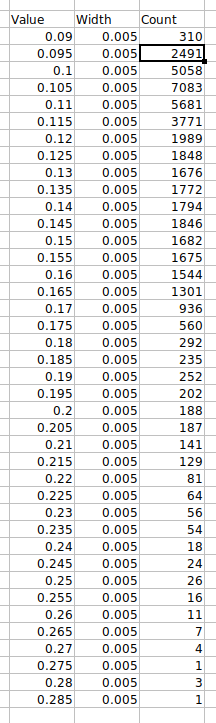
\includegraphics[width=\textwidth]{images/excel_data.png}
        \caption{Initial data}
        \label{fig: initial data}
    \end{subfigure}
    \hfill
    \begin{subfigure}{.74\textwidth}
        \centering
        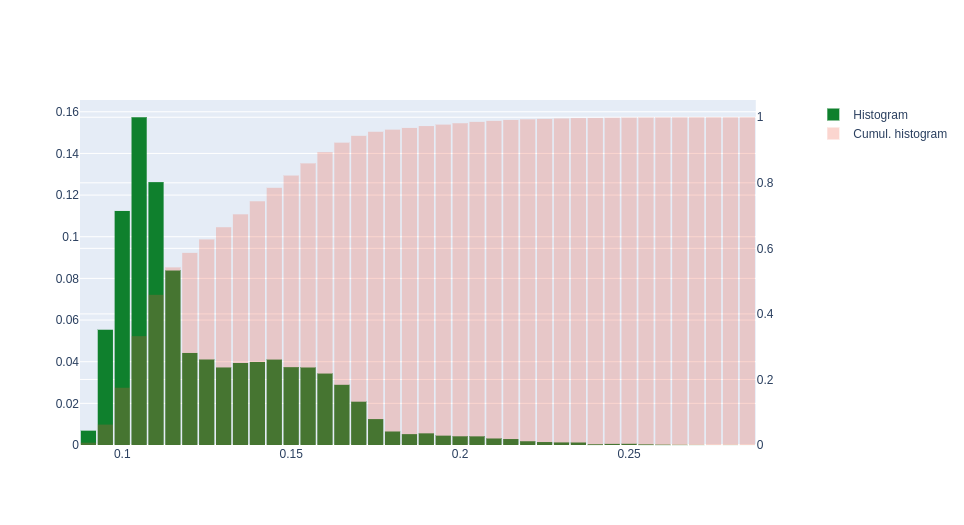
\includegraphics[width=\textwidth]{images/plot_excel_data.png}
        \caption{Visual representation of the initial data}
        \label{fig: visual representation of the initial data}
    \end{subfigure}
    \caption{A look at the initial data}
\end{figure}

\section{Bootstrap}
\label{section: bootstrap}
We use the bootstrap to estimate the confidence in the computed quantiles, even with small to moderate sample size.

Let \(n\) be the size of the data at our disposal and let \(q_k\) be the quantile we want to compute. Here is how we proceed:
\begin{enumerate}
    \item Do the following \(R\) times.
          \begin{enumerate}
              \item Draw a random sample of size \(n\) with replacement from the initial data.
              \item Compute \(q_k\) on the sample which has just been drawn. \label{bootstrap repeated step}
          \end{enumerate}
    \item Compute the mean over the set of values resulting from step \ref{bootstrap repeated step}.
    \item Compute the confidence intervals (details in section \ref{section: confidence intervals on the bootstrap})
\end{enumerate}

The plots in figure \ref{fig: estimation of quantiles} show the evolution of our estimate for the value of the quantiles as we go through replicates of the bootstraps. The grey areas represent the $95\%$ confidence intervals during that evolution. We will see how to get the confidence intervals from our histogram in section \ref{section: confidence intervals on the bootstrap}.

\begin{figure}
    \centering
    \begin{subfigure}{.84\textwidth}
        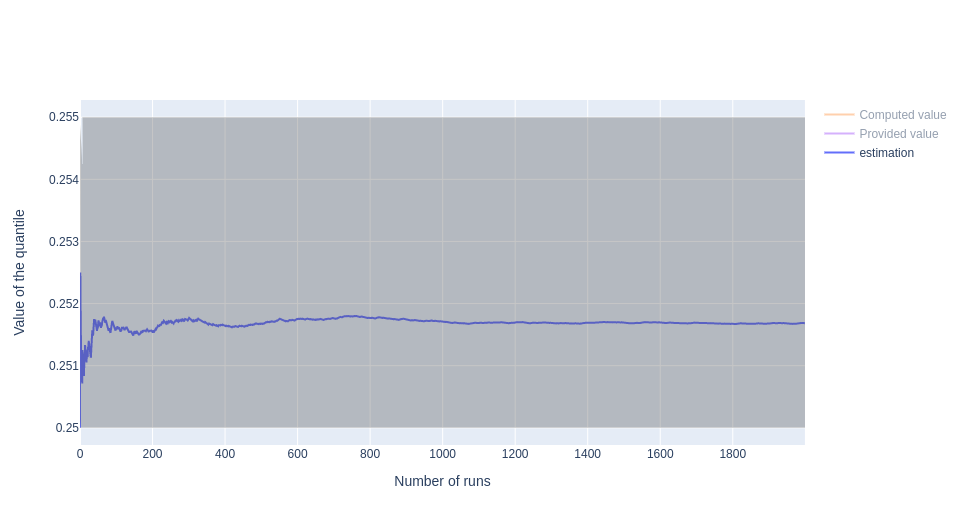
\includegraphics[width=\textwidth]{images/estimation_q3.png}
        \caption{Estimation of $q_3$}
    \end{subfigure}
    \hfill
    \begin{subfigure}{.84\textwidth}
        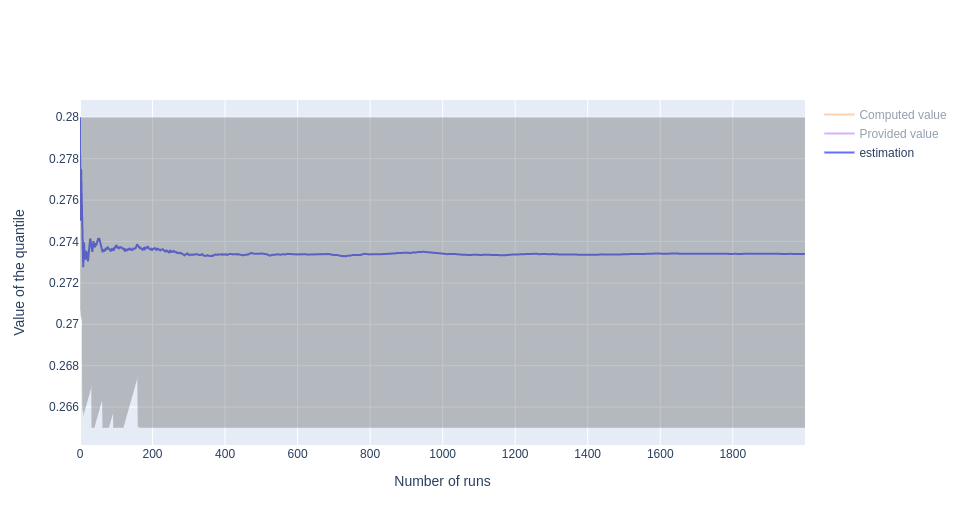
\includegraphics[width=\textwidth]{images/estimation_q4.png}
        \caption{Estimation of $q_4$}
    \end{subfigure}
    \hfill
    \begin{subfigure}{.84\textwidth}
        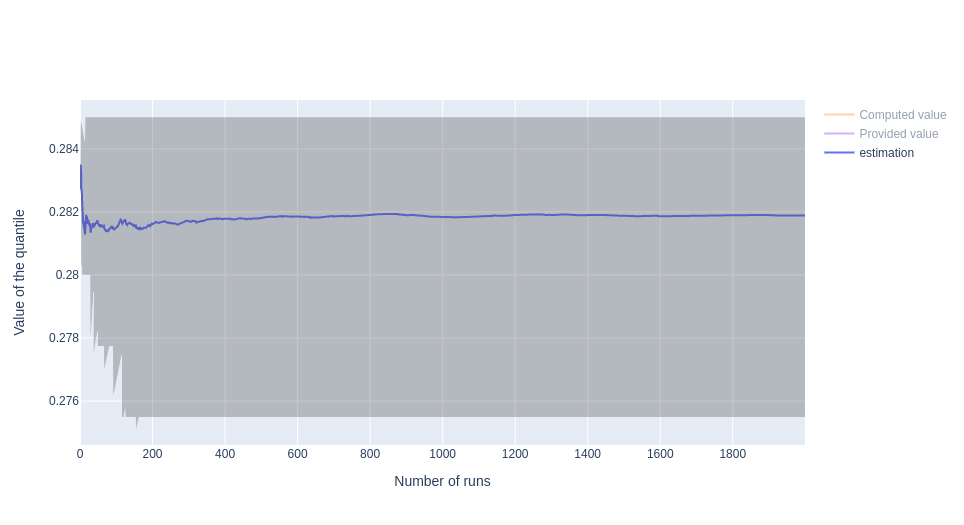
\includegraphics[width=\textwidth]{images/estimation_q5.png}
        \caption{Estimation of $q_5$}
    \end{subfigure}
    \caption{Estimation of the quantiles over bootstrap replicates}
    \label{fig: estimation of quantiles}
\end{figure}

\section{Confidence intervals on the bootstrap}
\label{section: confidence intervals on the bootstrap}

Let us assume that we want to compute the $95\%$ confidence interval. \\
First, let us note the following:
\begin{equation}
    \label{eq: compute 0.95 CI bounds}
    \frac{1 - 0.95}{2} = 0.025 \qquad \mbox{and} \qquad 1 - \frac{(1 - 0.95)}{2} = 0.975
\end{equation}

Now we compute the $95\%$ confidence interval. First, we sort the set of all the $q$'s that have been computed for each individual sample. Then we take the 0.025-th and 0.975-th quantile respectively as our lower-bound and upper bound for the confidence intervals. \\
More generally, for a $\gamma$-confidence interval (instead of $95\%$), one has that the lower and upper bounds of the confidence interval are respectively
\[
    \gamma_{lo} := \frac{1 - \gamma}{2} \qquad \mbox{and} \qquad \gamma_{up} := 1 - \frac{(1 - \gamma)}{2}
\]


\textbf{According to our data}, it seems that there is close to no change in the estimation of the quantiles after $1000$ replications of the bootstrap. The variations are small after 500 replicates already but for safety purposes we consider that we have our final guess after 1000 replicates. As for the confidence intervals, only in some edge cases do we have changes past the 1000 mark. \\
The fact that our estimate seems to be stable after \(1000\) replicates does not matter for the number \(1000\) itself. However, it matters because we seem to ``converge" to some value and reach a final value.

\textit{NB: Our estimate of 1000 replicates is based on empirical evidence. It is not a theoretical result, however, we believe that it is suitable for engineering purposes.}

\textbf{According to the litterature}, that is according to Jean-Yves Le Boudec's \textit{Performance Evaluation of Computer and Communication Systems}, there exists some ``good value" for the number of bootstrap replicates \(R\). With \(\gamma\) being the confidence level, Le Boudec advises to choose \(R\) as follows
\begin{equation}
    R = \frac{50}{1 - \gamma} - 1
\end{equation}
therefore for \(\gamma = 95\% = 0.95\) we deduce that the value of \(R\) is

\begin{align*}
    R & = \frac{50}{1 - 0.95} - 1 \\
      & = 1000 - 1                \\
      & = 999                     \\
\end{align*}

We find that our estimates verifies Le Boudec's result (1000 compared to 999).


\section{Conclusion}

The in-depth study in the main body of this article, as well as the supplementary tests provided in appendix \ref{app: supplementary tests on other datasets} show a wide variety in the amounts of data at our disposal. The simulation times are 24 seconds, 4 minutes, 40 minutes and 400 minutes; in other words, 24 seconds times powers of 10, which gives an overview over multiple orders of magnitude. The number of data points ranges from a mere 1355 to almost 24 000 000 depending on the simulation time and the test case. The distributions themselves are very different too, some have well-spread values while others are very narrowly concentrated. As a result, we get some fairly contrasted results.

We notice that simulation times of 24 seconds appear too short and the results usually get better for 4, 40 and 400 minutes. However, and this is more surprising, in some cases, 400 minutes of simulation appear to yield worse results than 4 or 40 minutes (figure \ref{fig: TFTP4 DAT q3 400 min} for example). Having few cases makes it hard to state whether this is an edge case or a general trend. However, besides some rare cases (such as figure \ref{fig: VD2 DAT q4 400 min}), the improvements between 40 and 400 minutes of simulation time do not seem substantial. On the other hand, performing the bootstrap on an order of magnitude more data points takes a far greater time. A vast portion of the runtime was dedicated to performing the bootstrap on the 400 minutes simulation times (about half of the total $\approx 48$ hours runtime on an 8-core i7-4710HQ CPU at 2.50GHz). In conclusion, it appears from our data that 4 to 40 minutes of simulation yields the best performance compared to runtime.


\newpage
\appendix
\section{Supplementary tests on other datasets}
\label{app: supplementary tests on other datasets}
To verify our approach and make sure that it generalises well, we test it on other datasets.

\subsection{CC1: CAM2 - ECU2}
\subsubsection{Data}

\begin{figure}[H]
    \centering
    \begin{subfigure}{.495\textwidth}
        \centering
        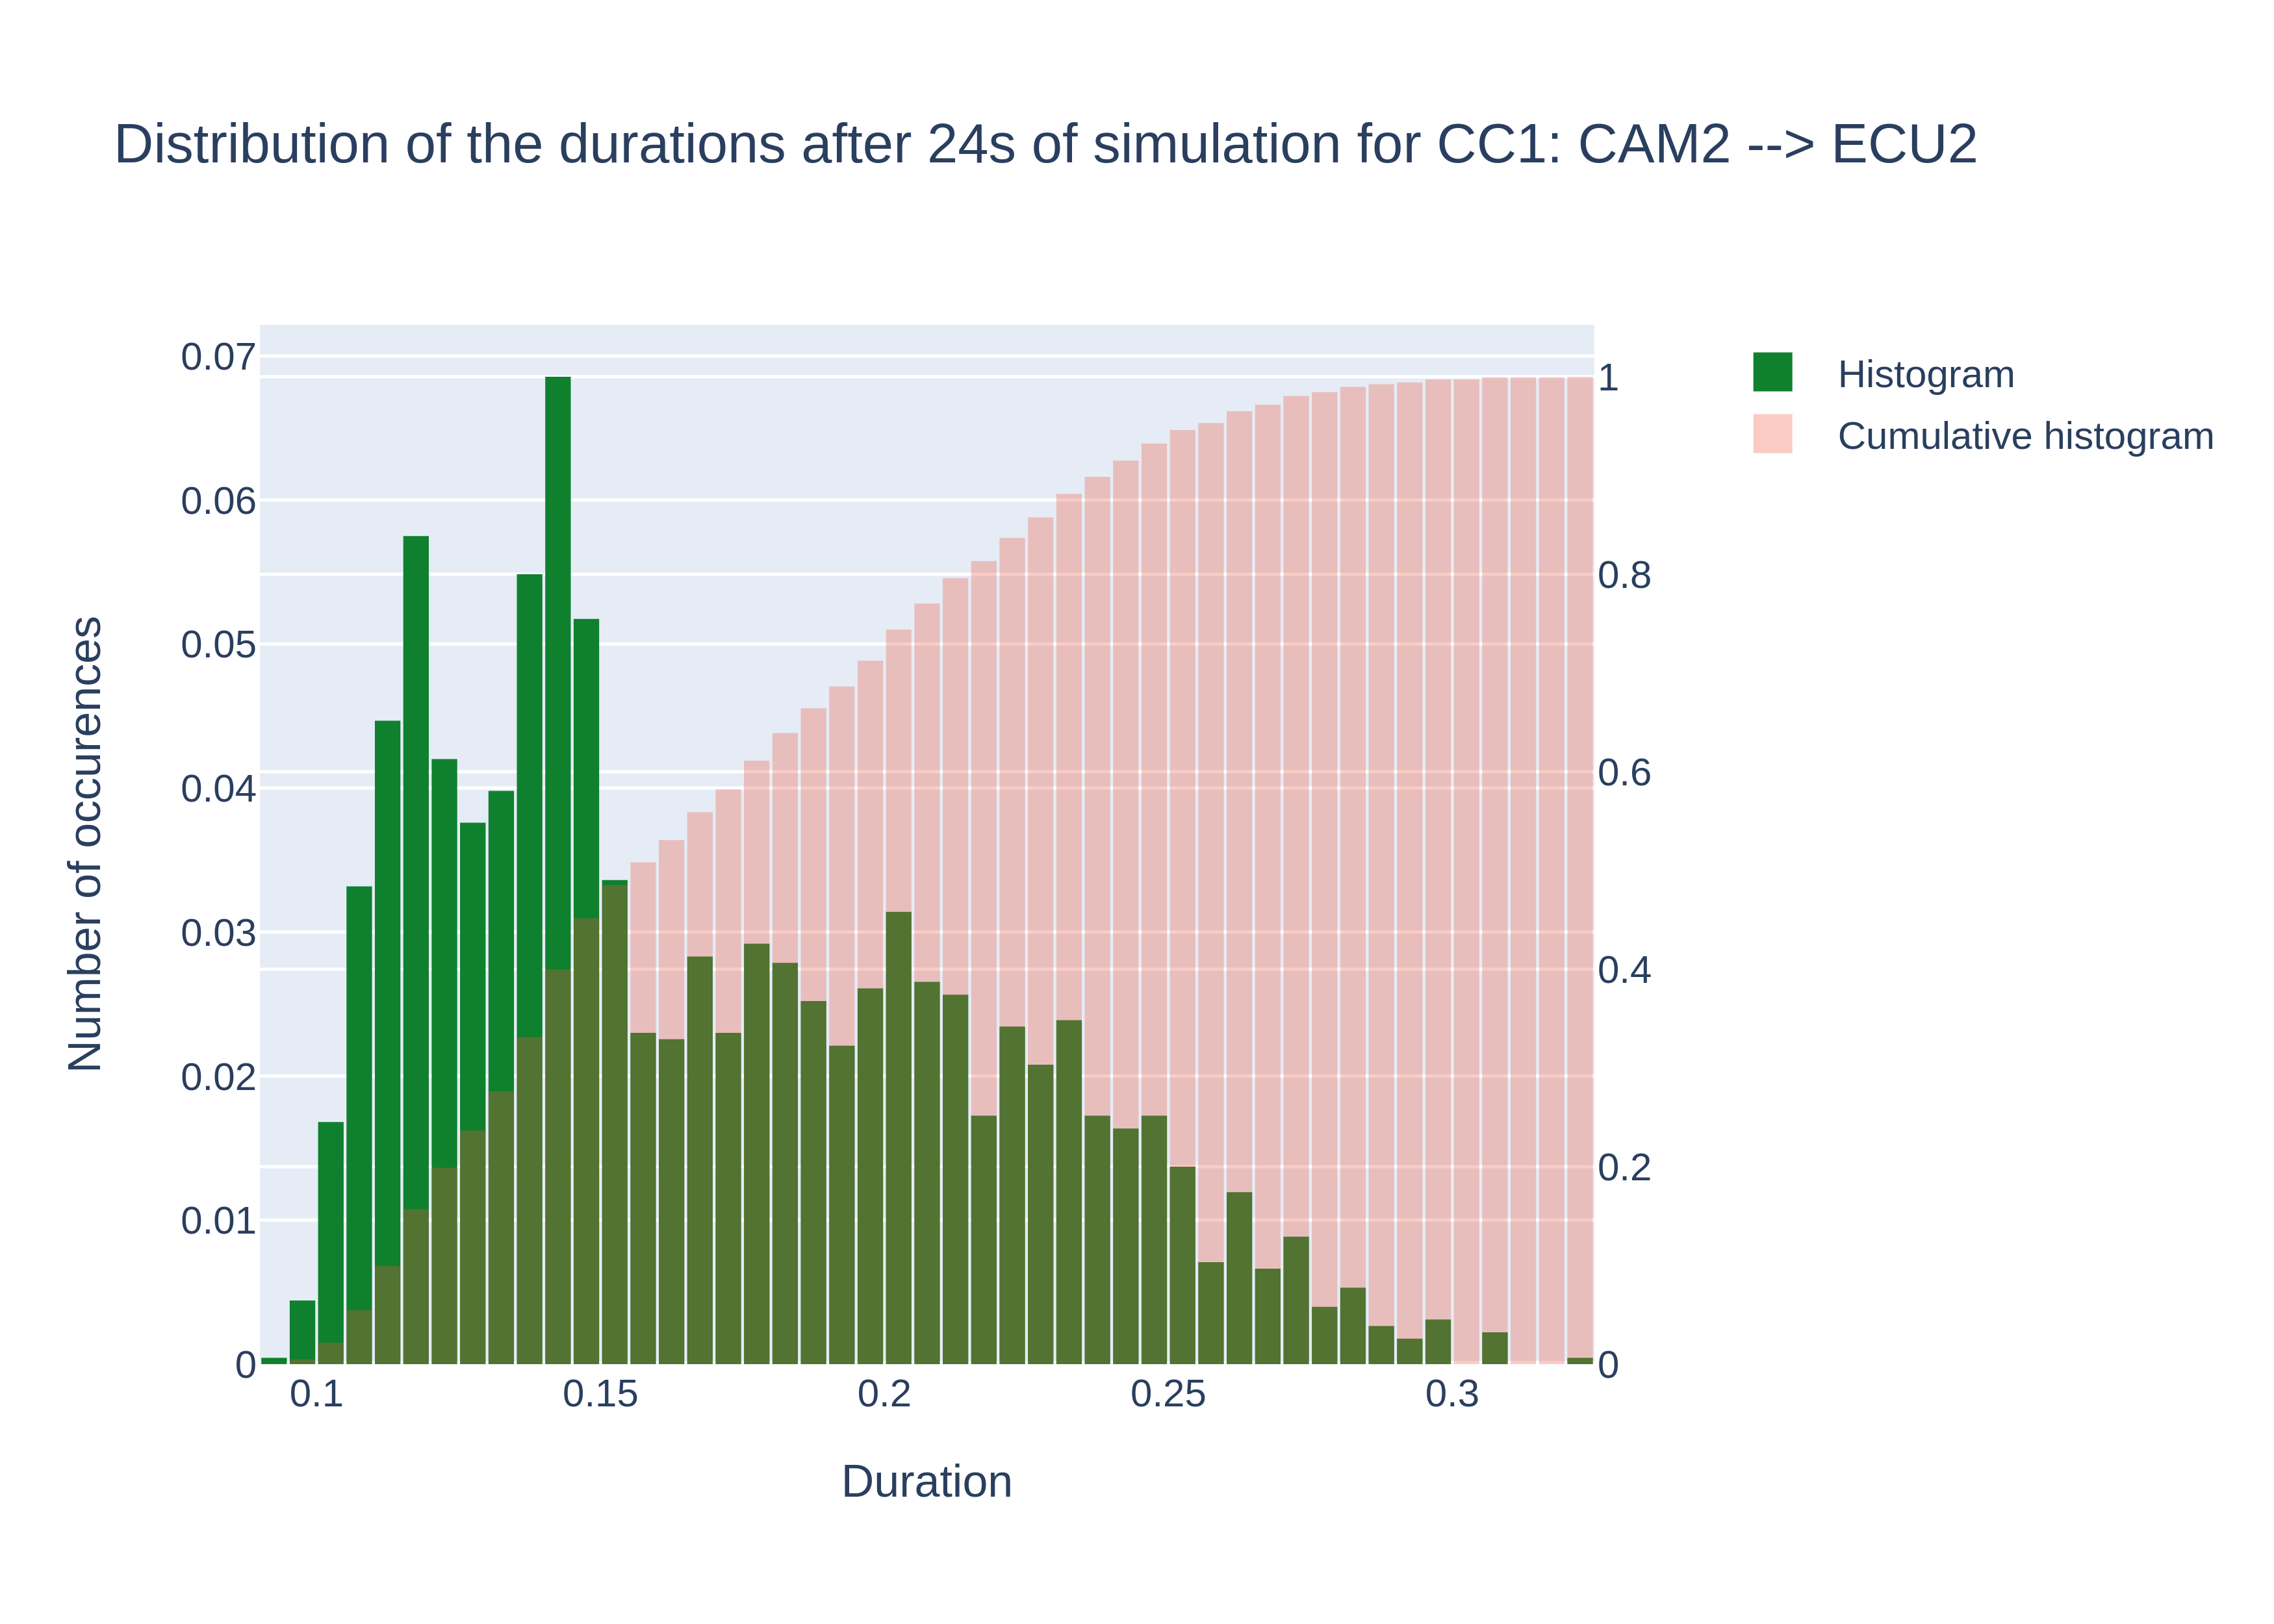
\includegraphics[width=\textwidth]{../fig/data/CC1: CAM2 --> ECU2_24s.png}
        \caption{Simulation time: 24s}
        \vspace{.5cm}
    \end{subfigure}
    \begin{subfigure}{.495\textwidth}
        \centering
        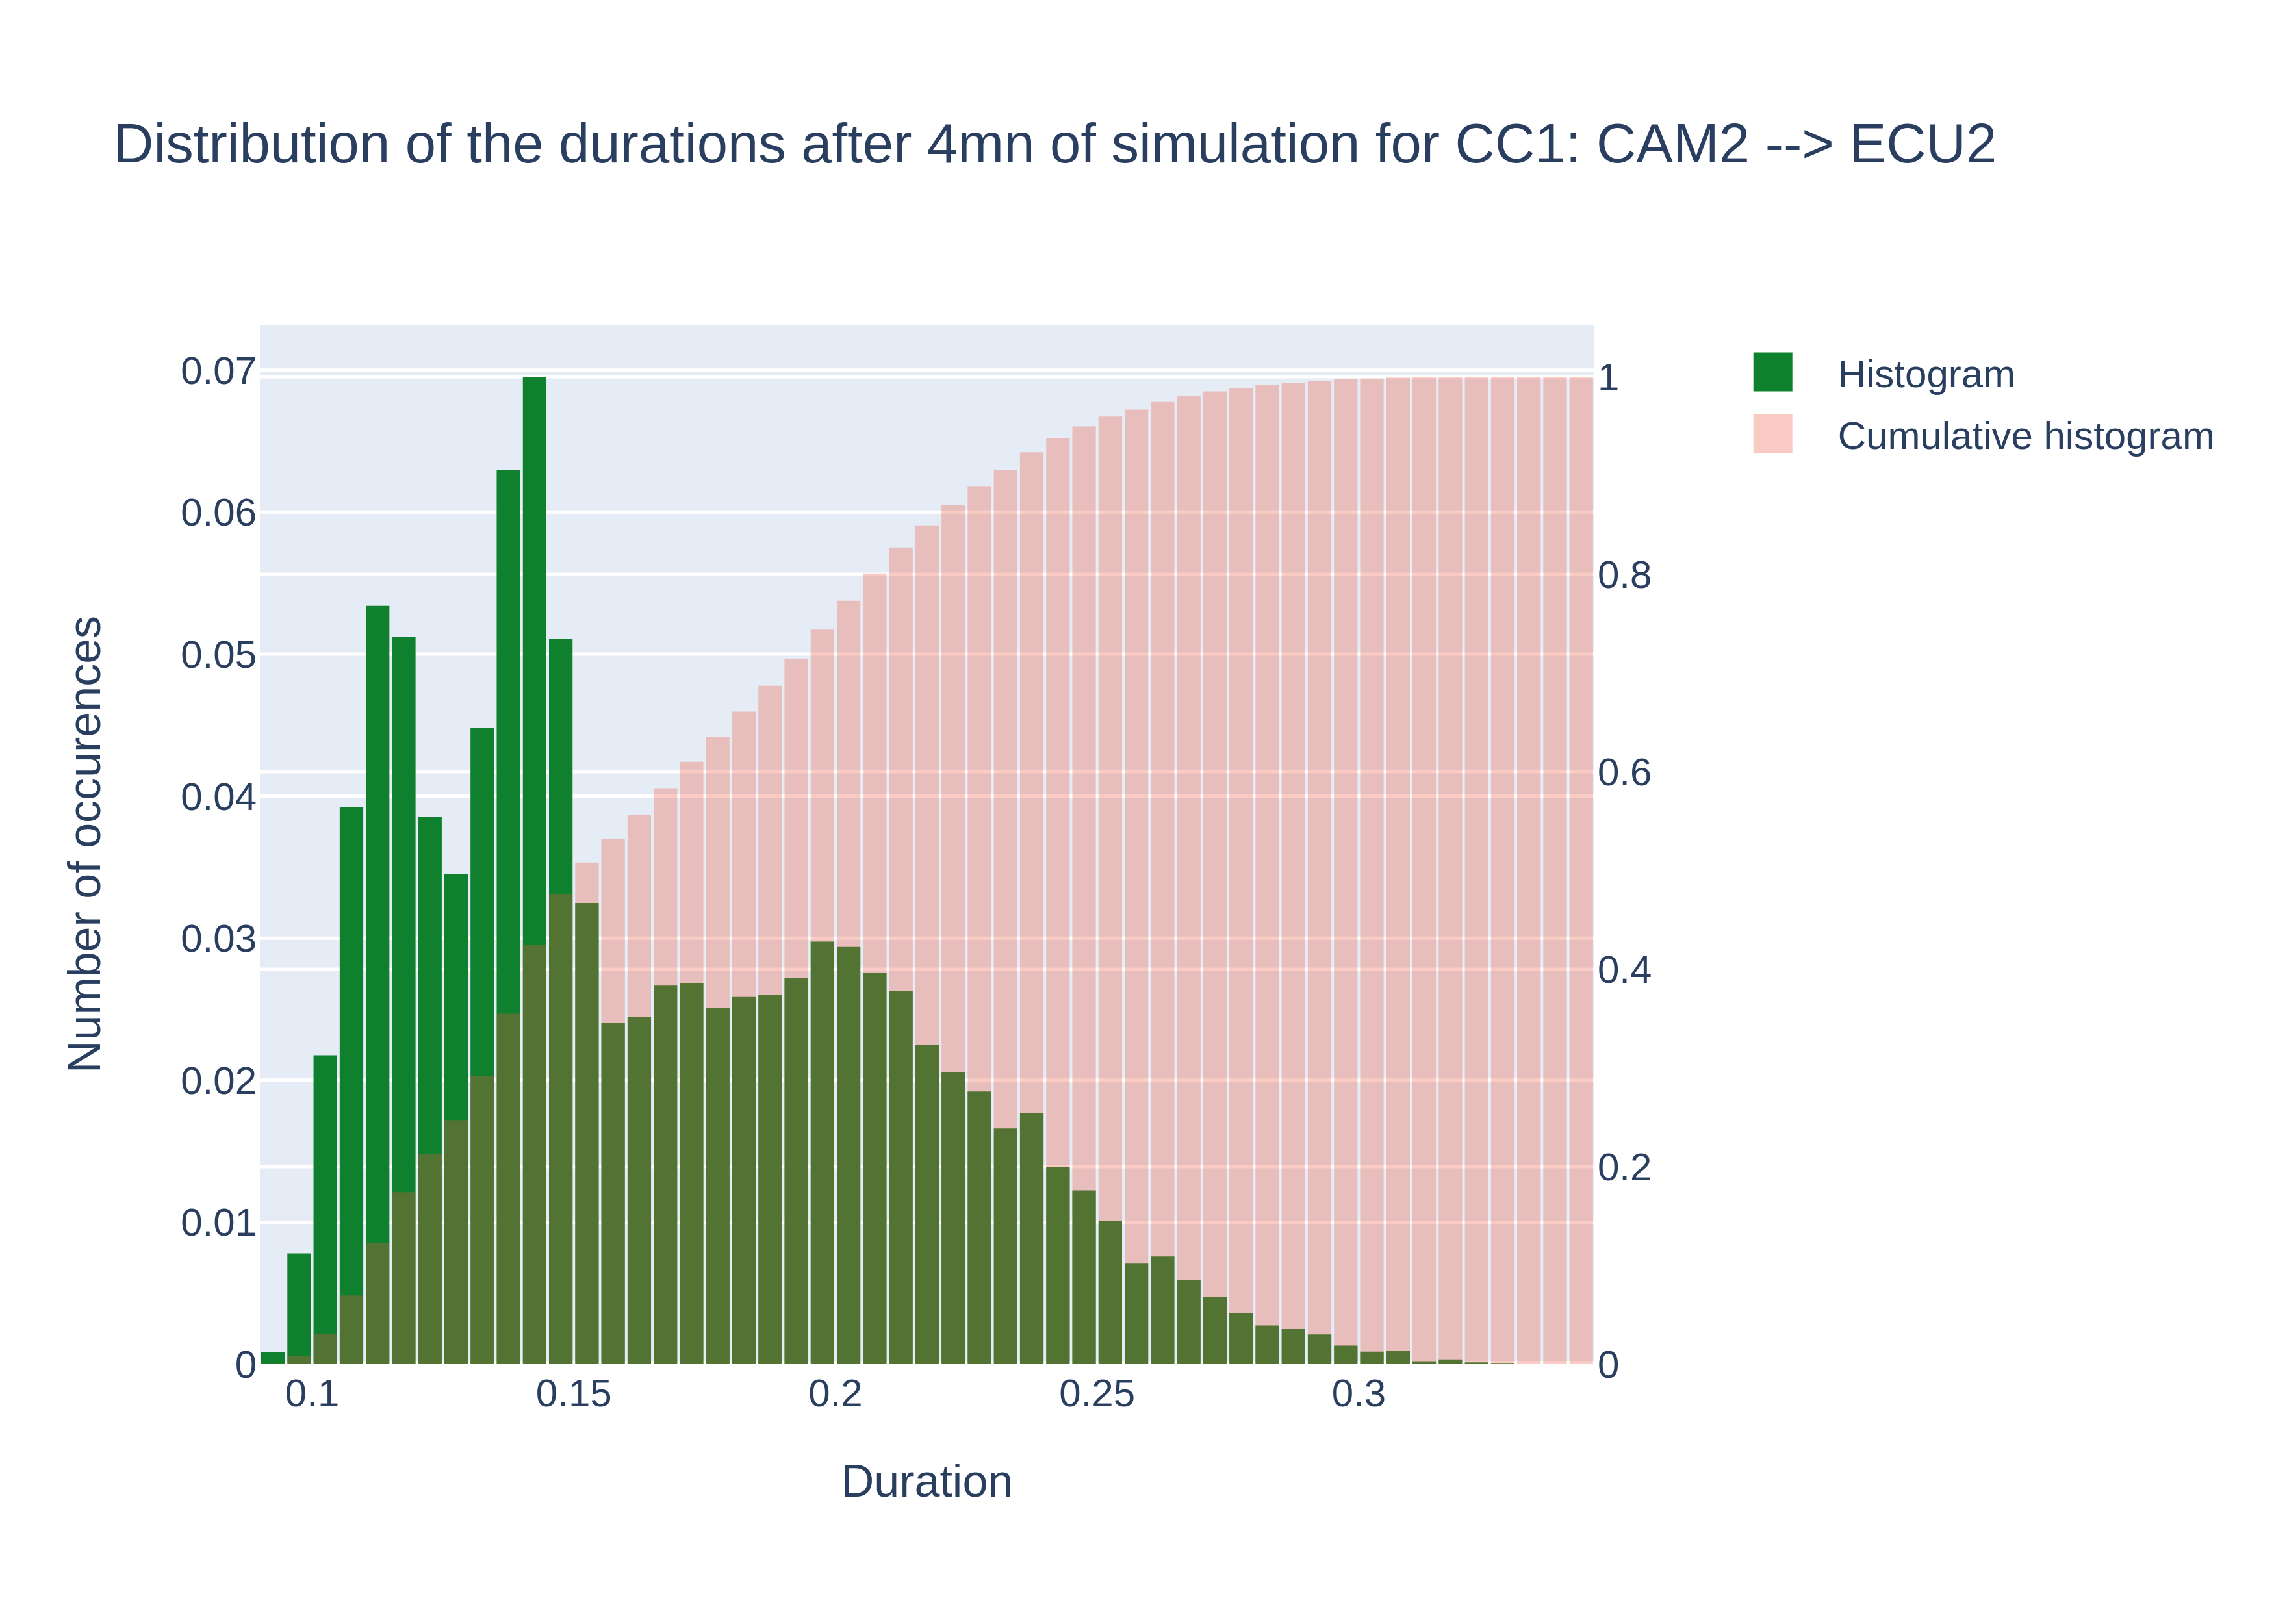
\includegraphics[width=\textwidth]{../fig/data/CC1: CAM2 --> ECU2_4mn.png}
        \caption{Simulation time: 4min}
        \vspace{.5cm}
    \end{subfigure}
    \begin{subfigure}{.495\textwidth}
        \centering
        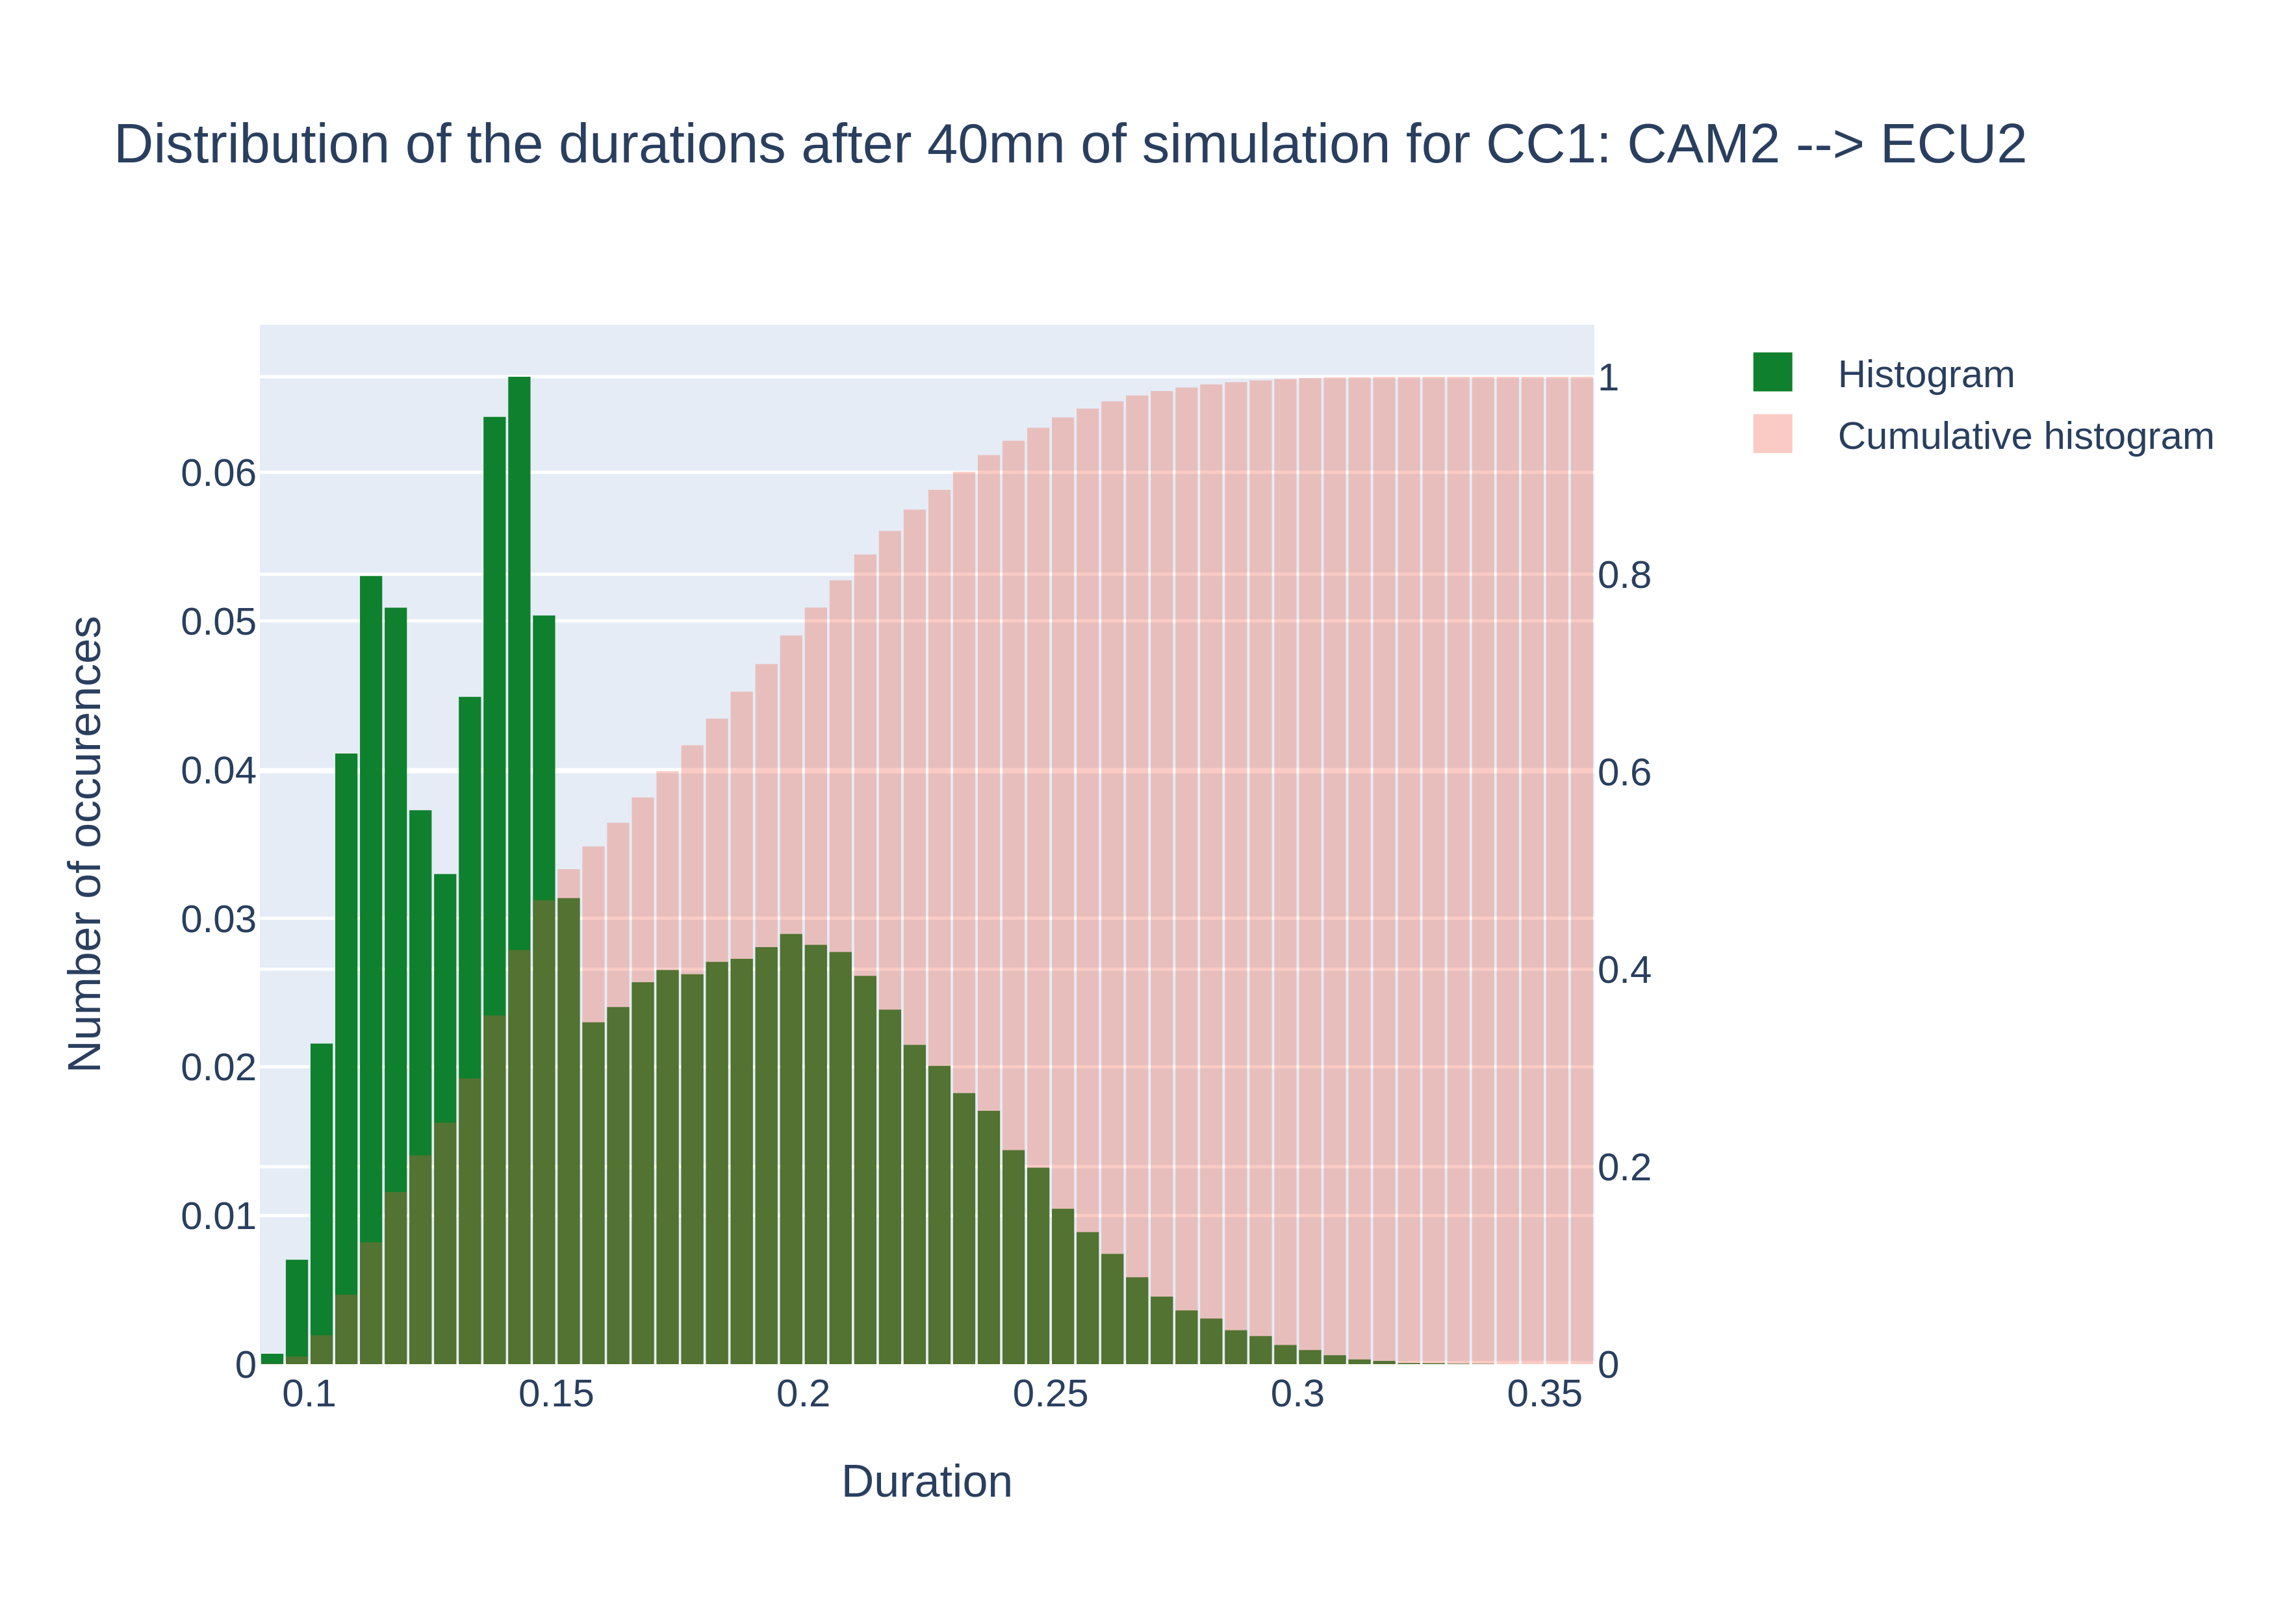
\includegraphics[width=\textwidth]{../fig/data/CC1: CAM2 --> ECU2_40mn.png}
        \caption{Simulation time: 40min}
    \end{subfigure}
    \begin{subfigure}{.495\textwidth}
        \centering
        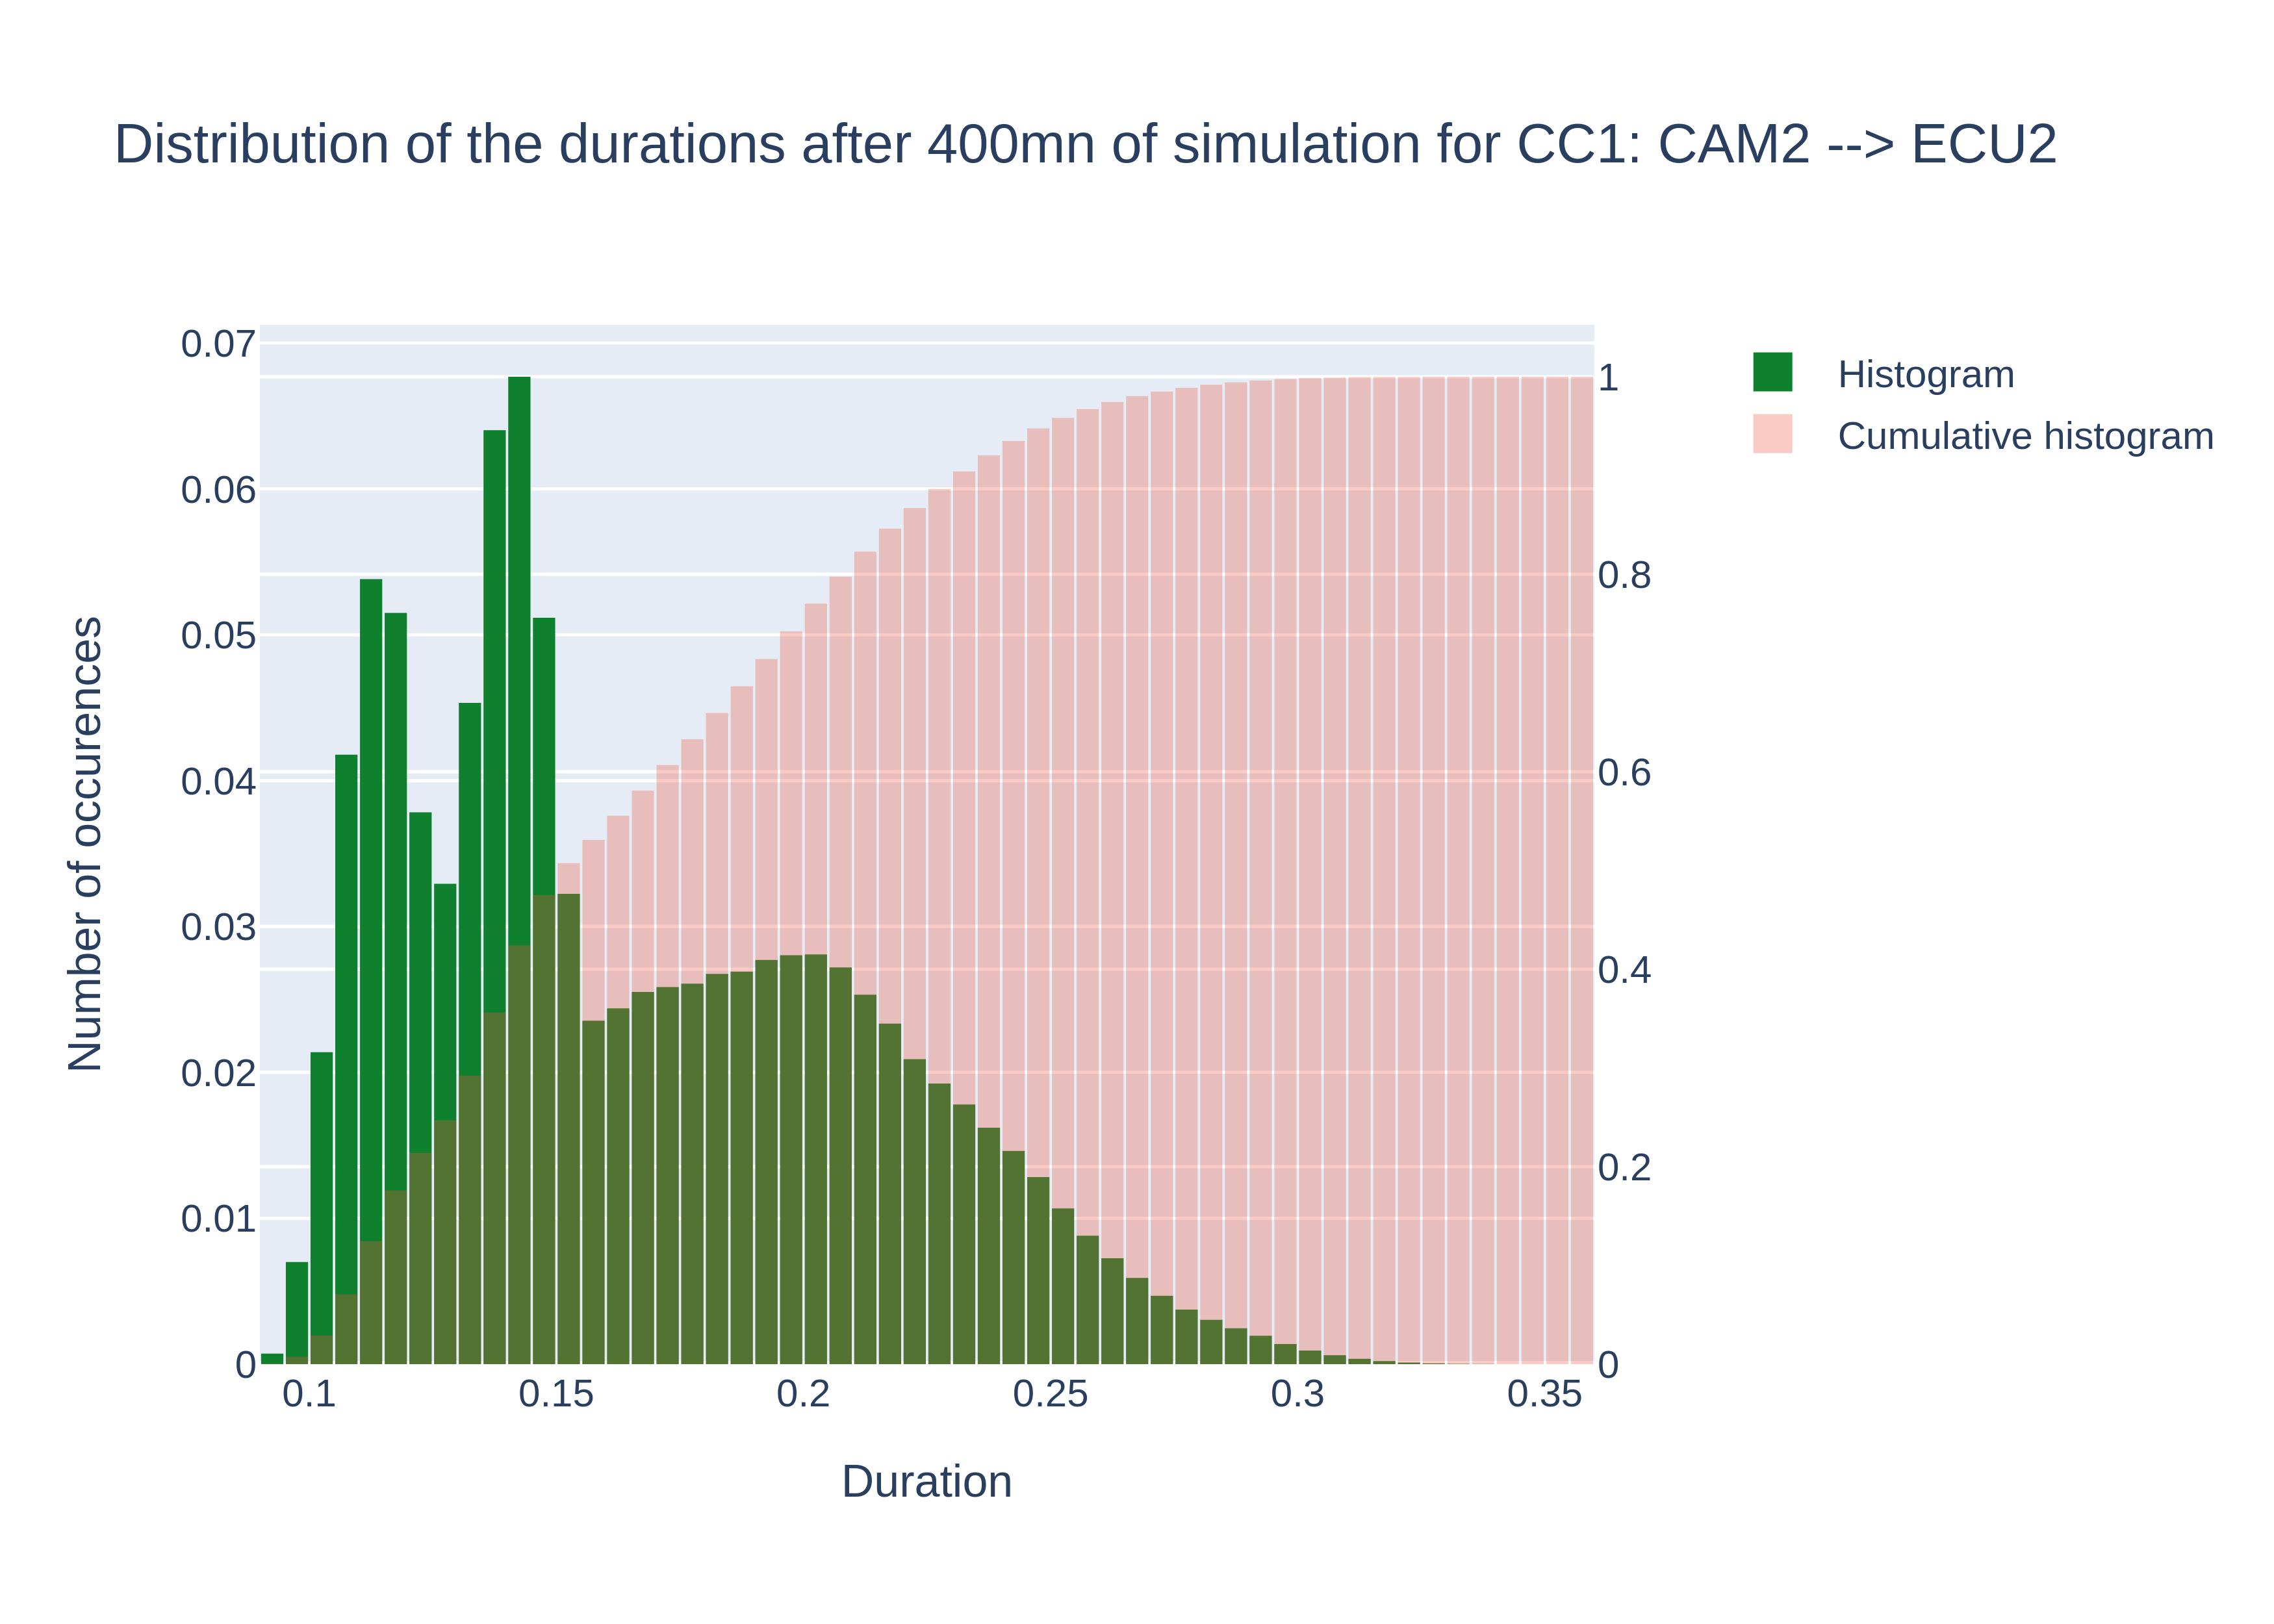
\includegraphics[width=\textwidth]{../fig/data/CC1: CAM2 --> ECU2_400mn.png}
        \caption{Simulation time: 400min}
    \end{subfigure}
    \caption{CC1: CAM2 - ECU2 data after multiple simulation times}
\end{figure}

\subsubsection{Quantile 3}
\begin{figure}[H]
    \centering
    \begin{subfigure}{.495\textwidth}
        \centering
        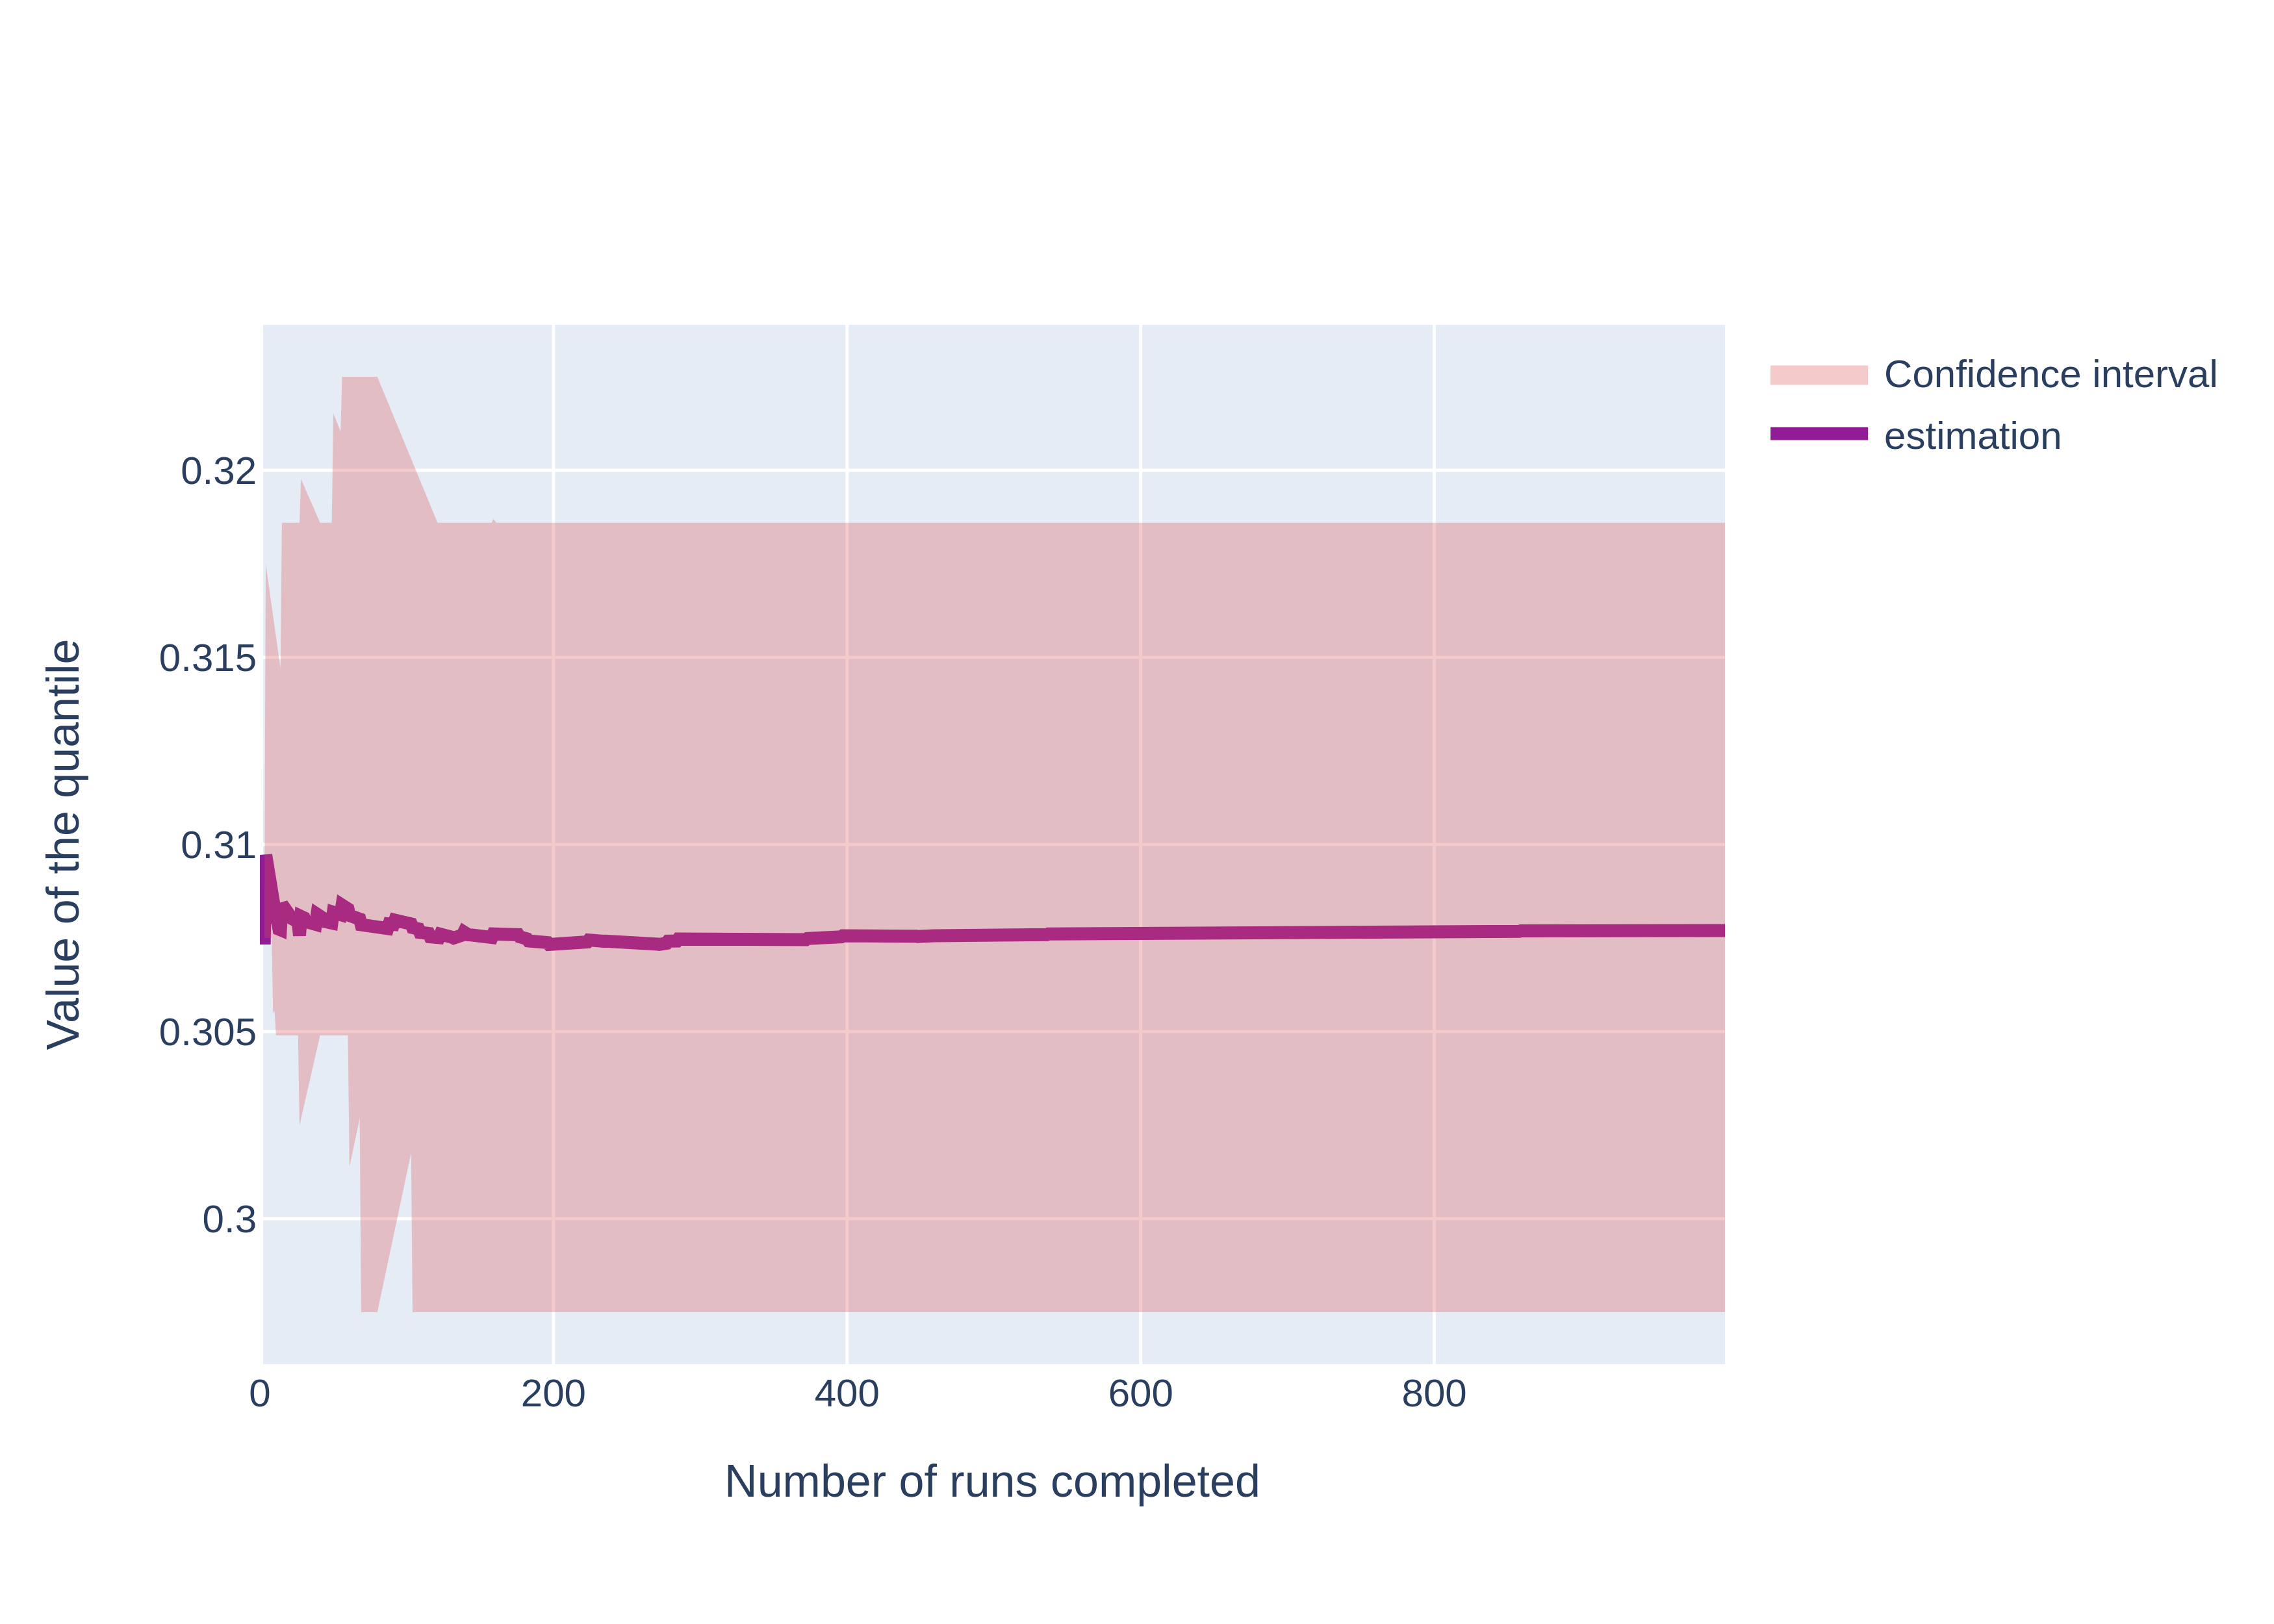
\includegraphics[width=\textwidth]{../fig/quantile3/CC1: CAM2 --> ECU2_24s.png}
        \caption{Simulation time: 24s}
        \vspace{.5cm}
    \end{subfigure}
    \begin{subfigure}{.495\textwidth}
        \centering
        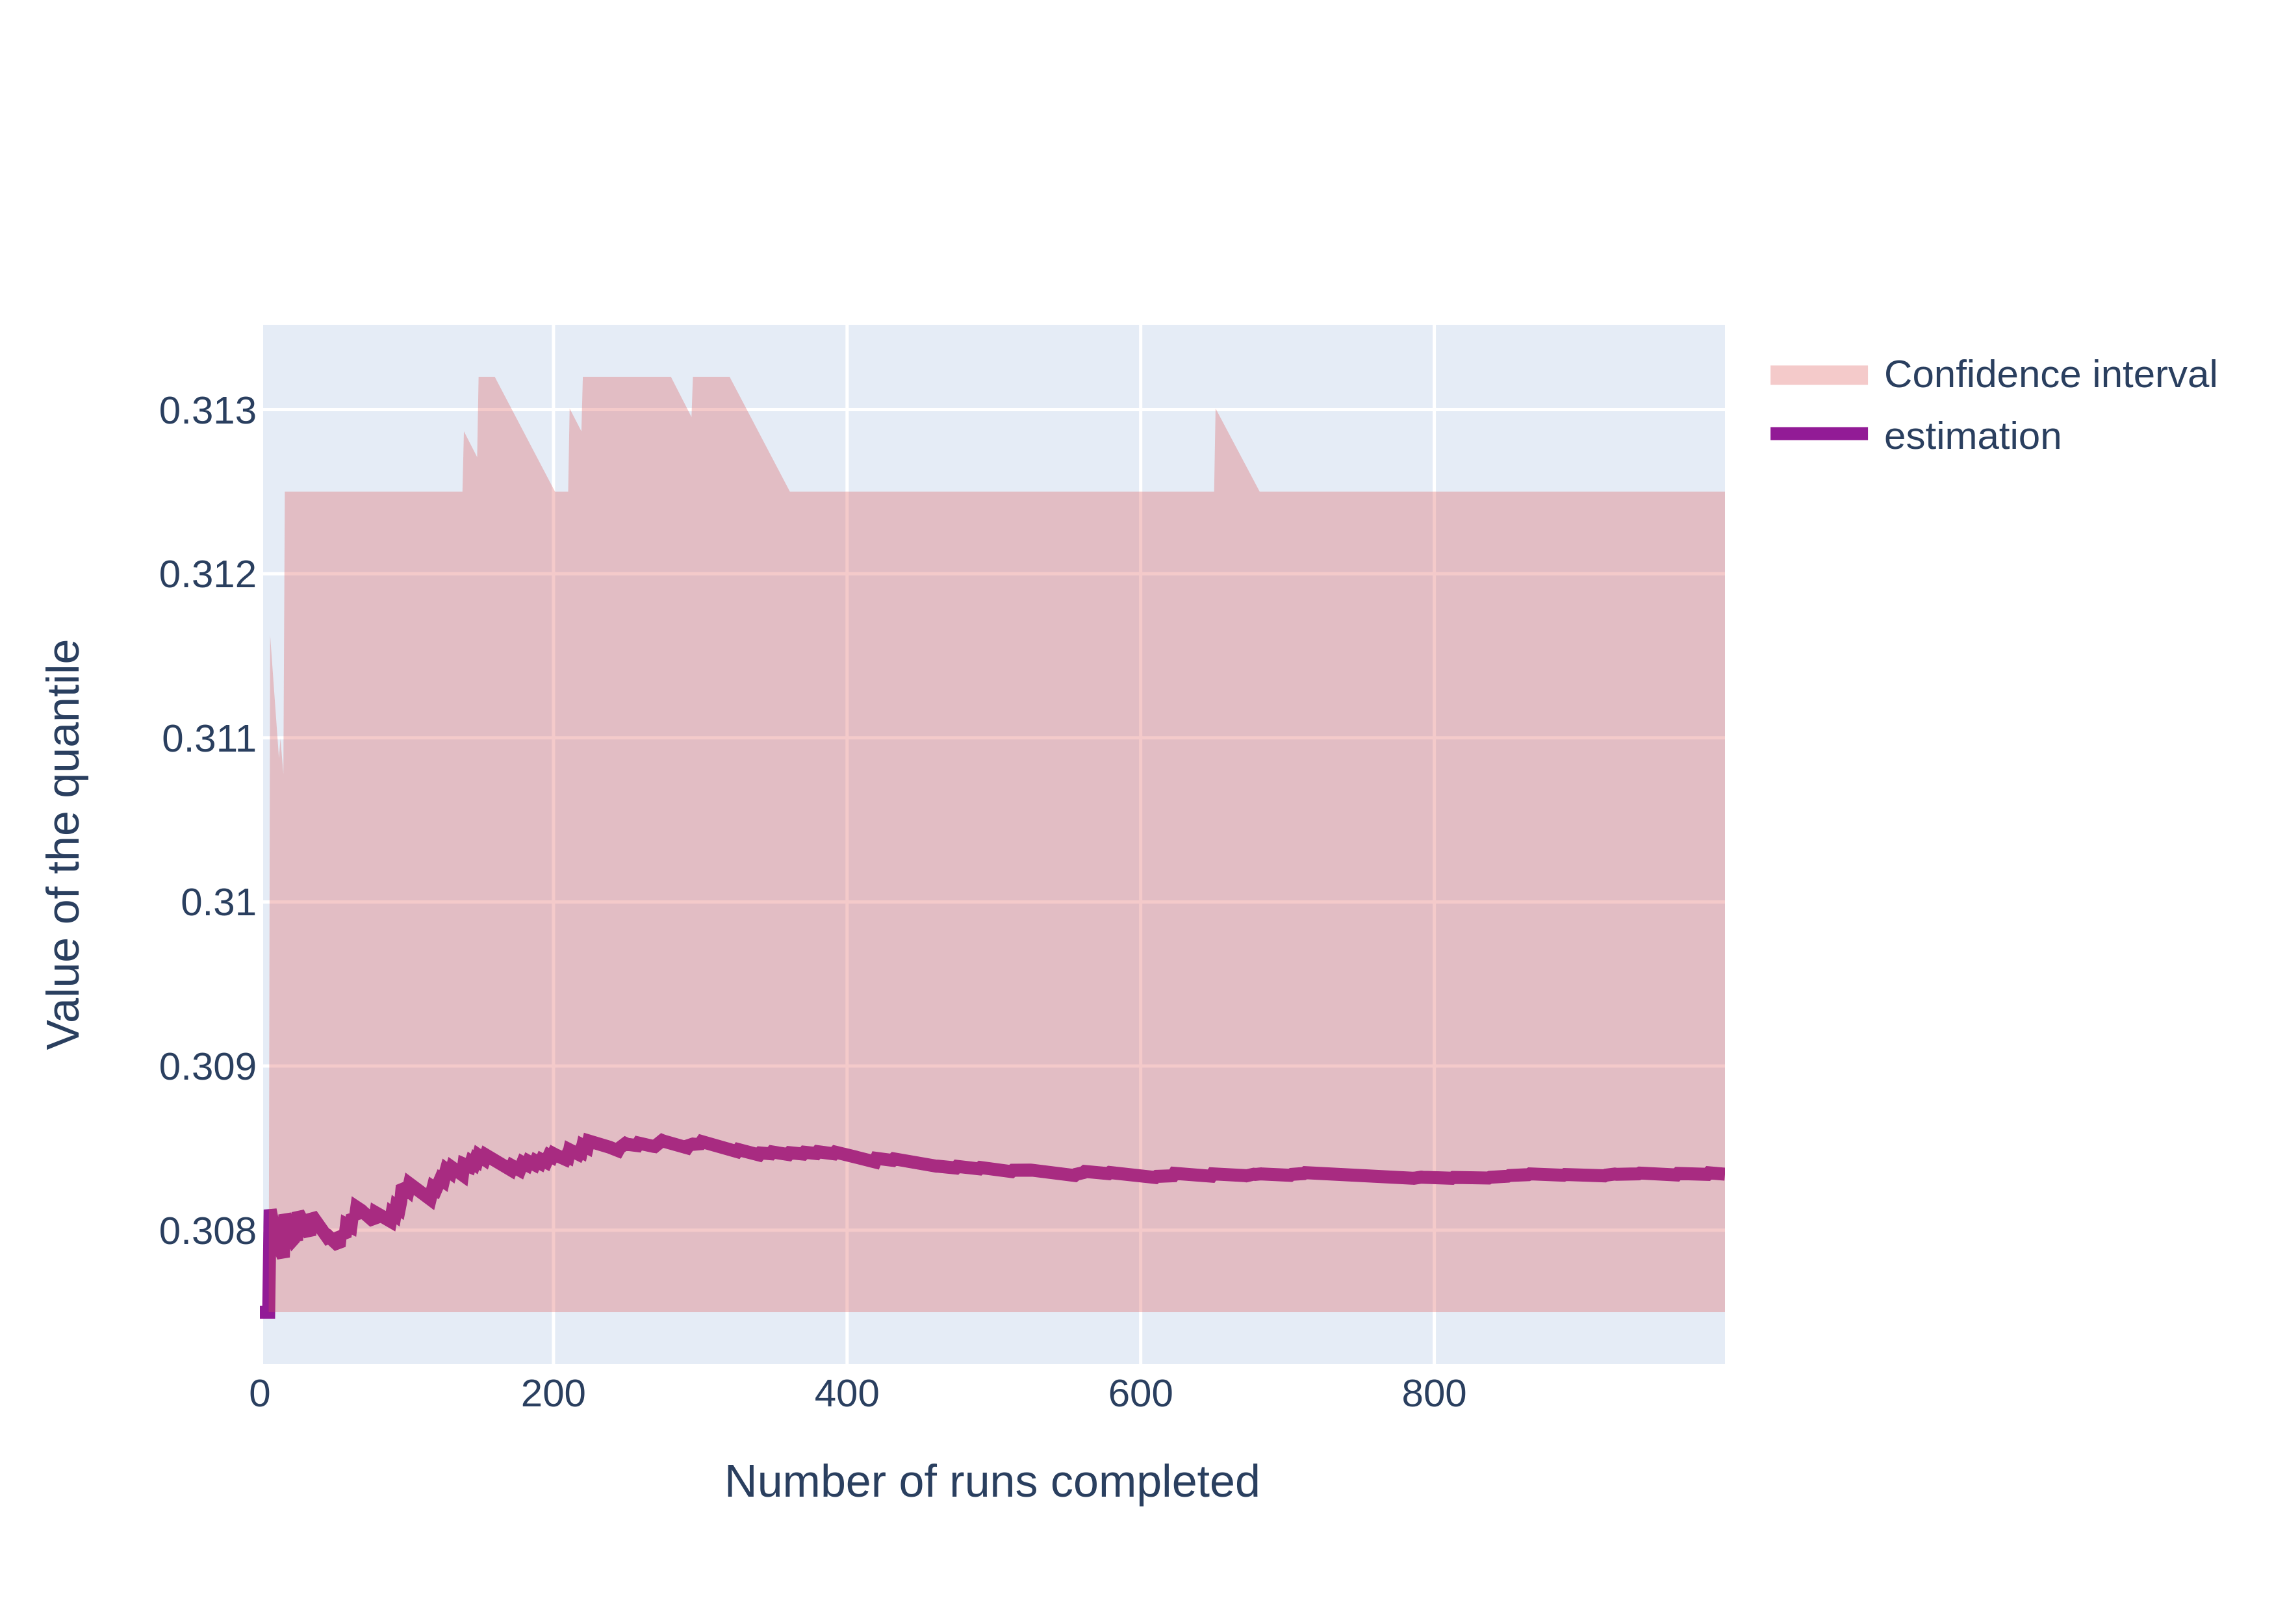
\includegraphics[width=\textwidth]{../fig/quantile3/CC1: CAM2 --> ECU2_4mn.png}
        \caption{Simulation time: 4min}
        \vspace{.5cm}
    \end{subfigure}
    \begin{subfigure}{.495\textwidth}
        \centering
        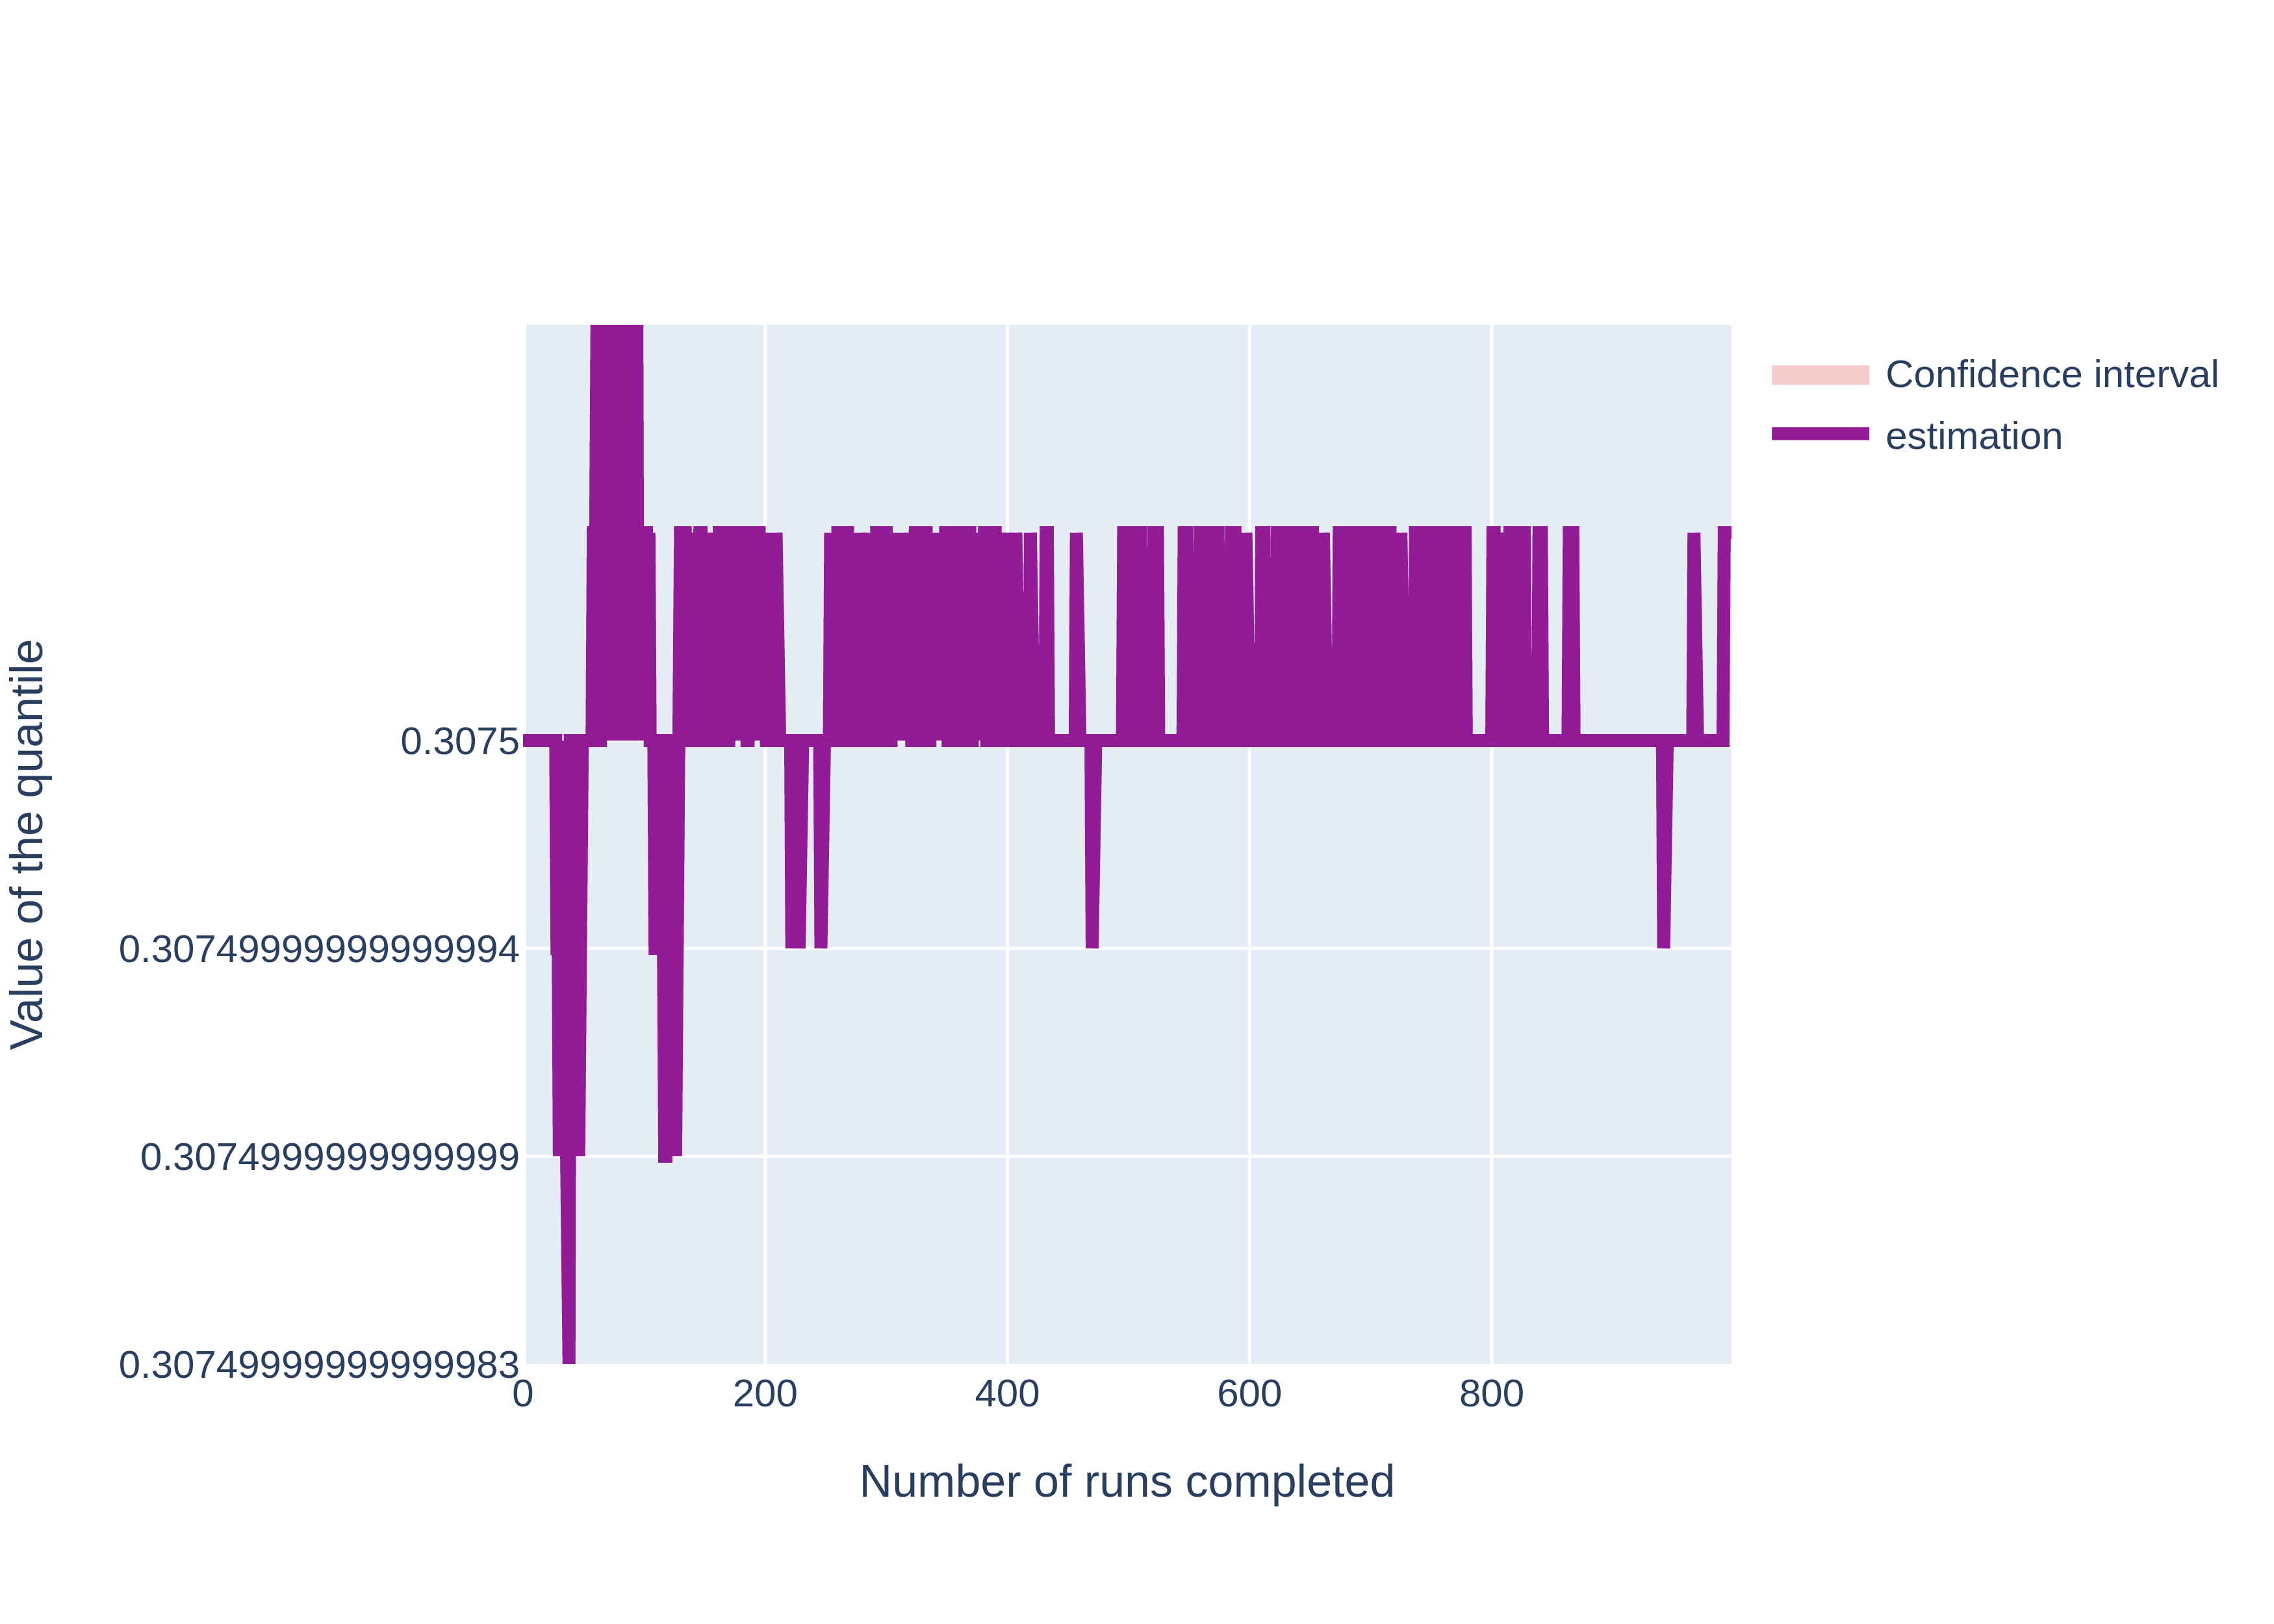
\includegraphics[width=\textwidth]{../fig/quantile3/CC1: CAM2 --> ECU2_40mn.png}
        \caption{Simulation time: 40min}
    \end{subfigure}
    \begin{subfigure}{.495\textwidth}
        \centering
        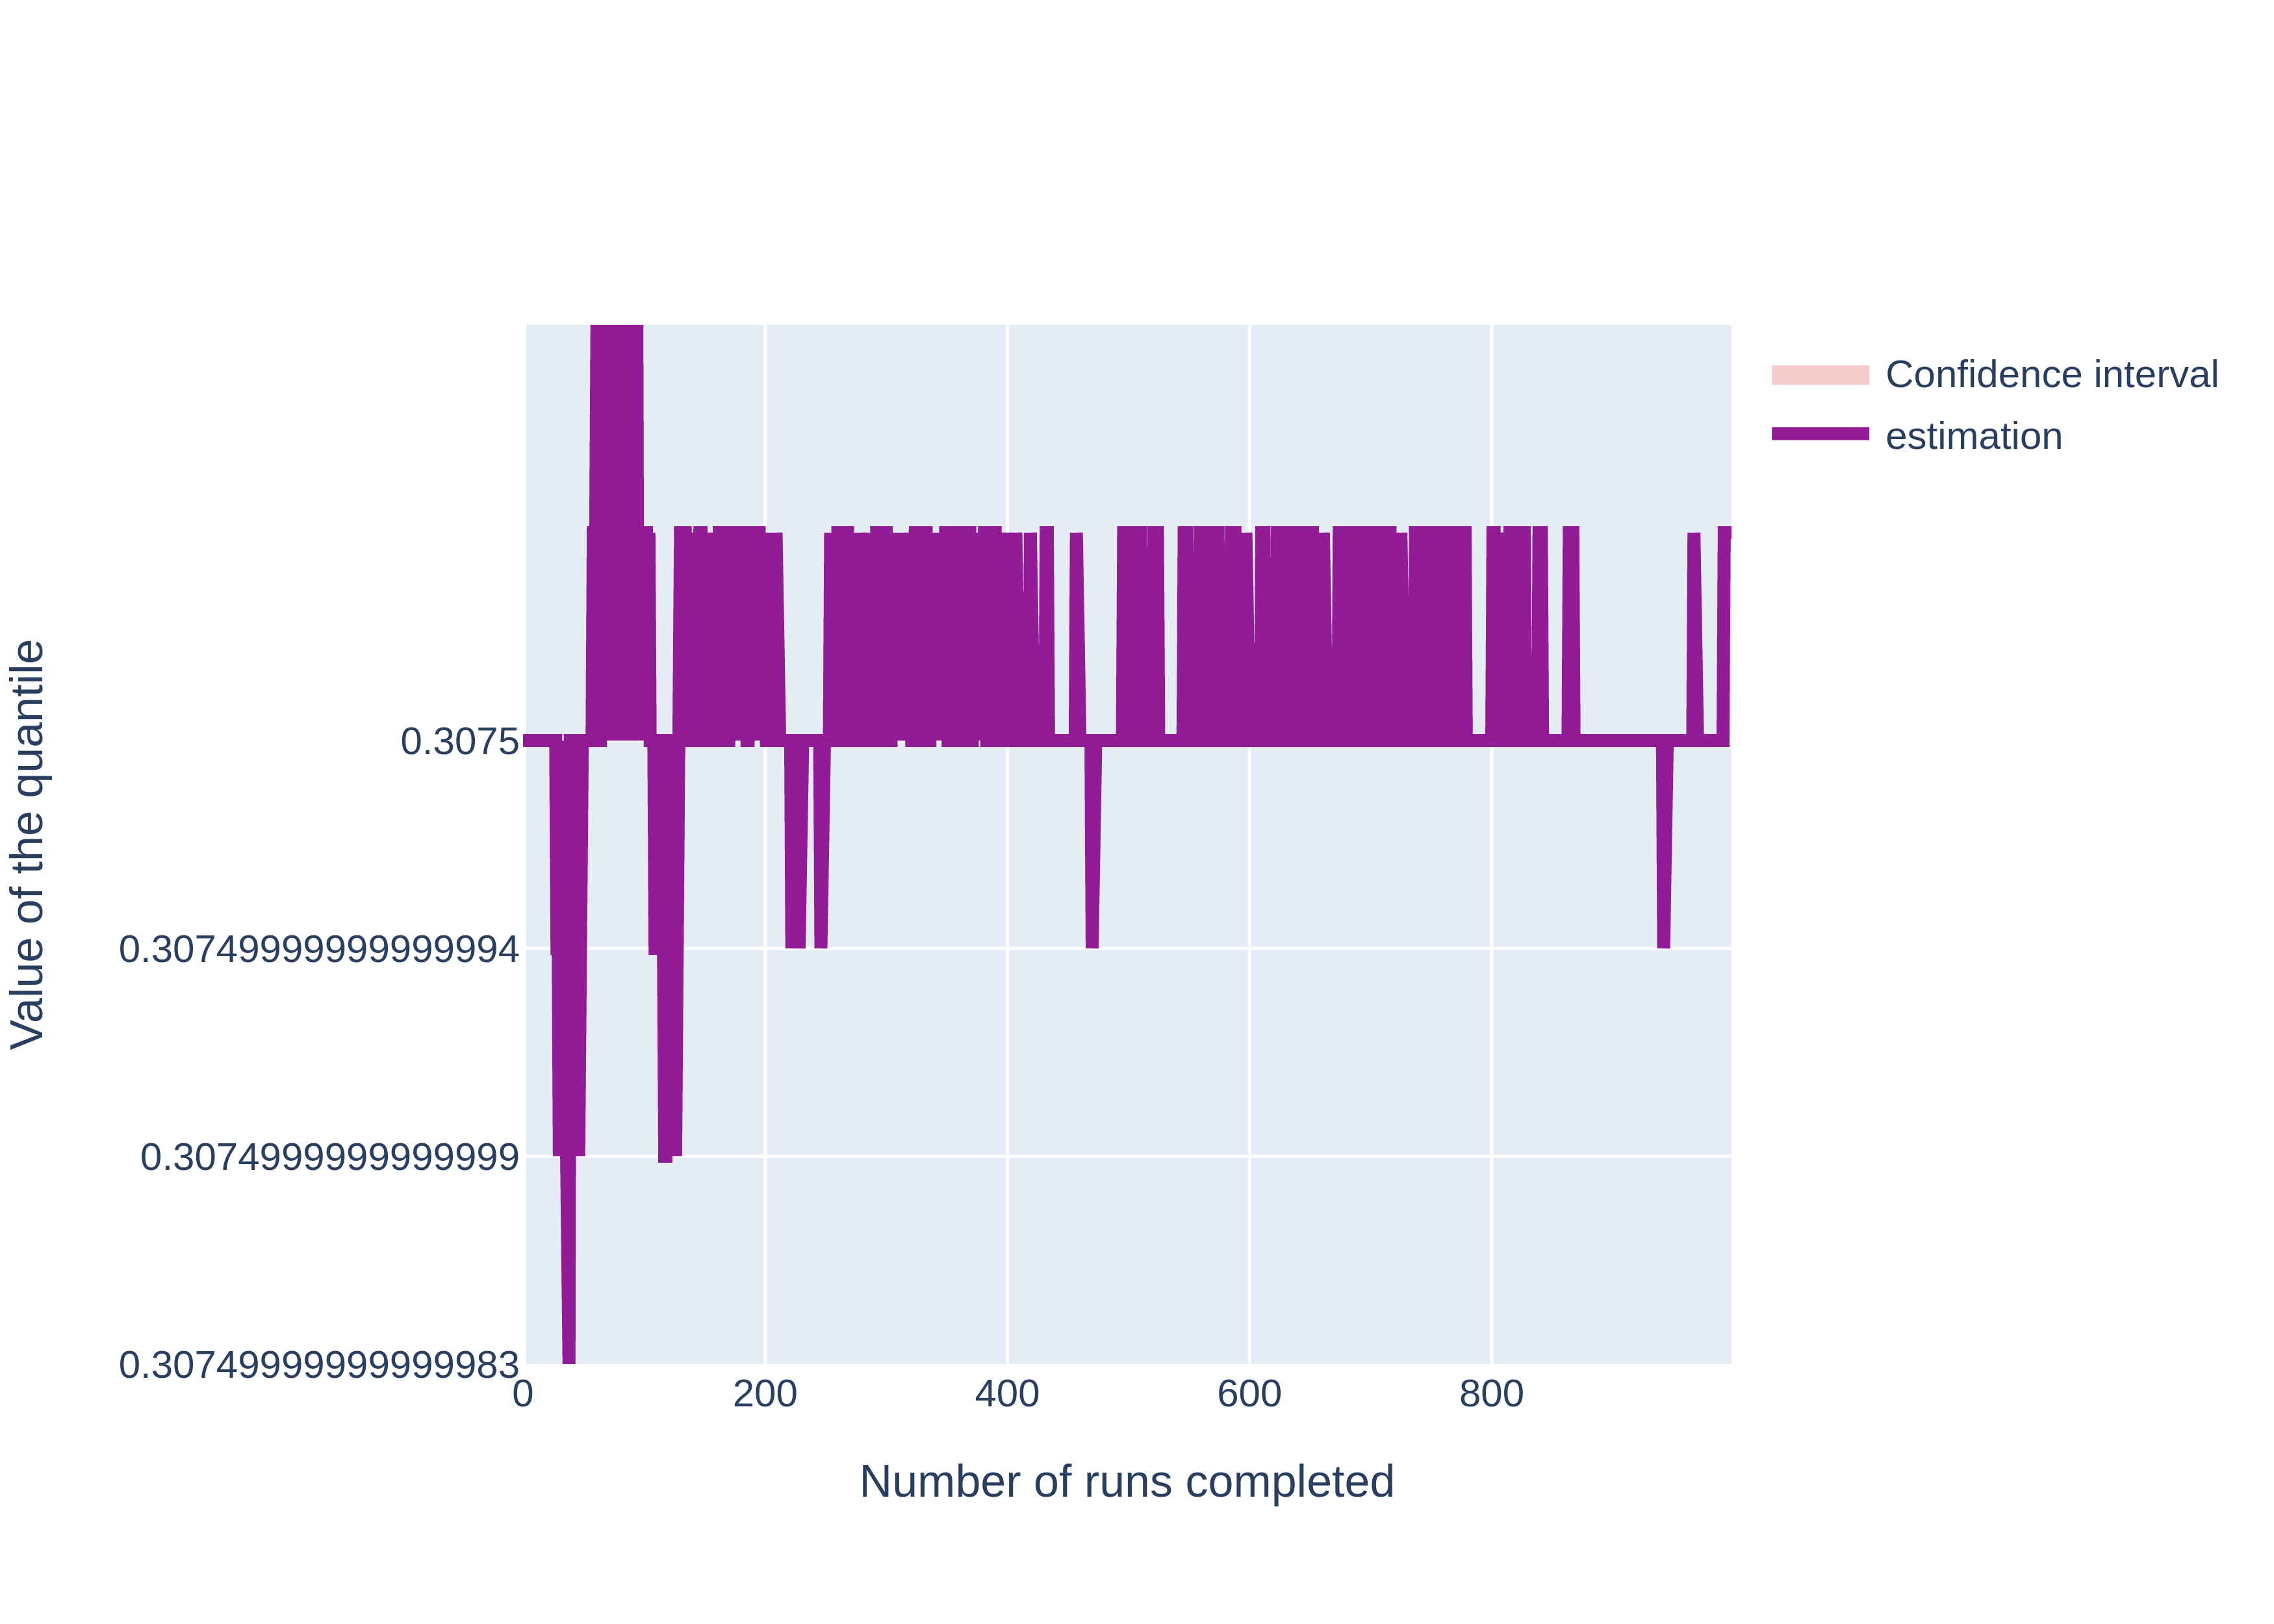
\includegraphics[width=\textwidth]{../fig/quantile3/CC1: CAM2 --> ECU2_400mn.png}
        \caption{Simulation time: 400min}
    \end{subfigure}
    \caption{CC1: CAM2 - ECU2 $q_3$ after multiple simulation times}
\end{figure}

\subsubsection{Quantile 4}
\begin{figure}[H]
    \centering
    \begin{subfigure}{.495\textwidth}
        \centering
        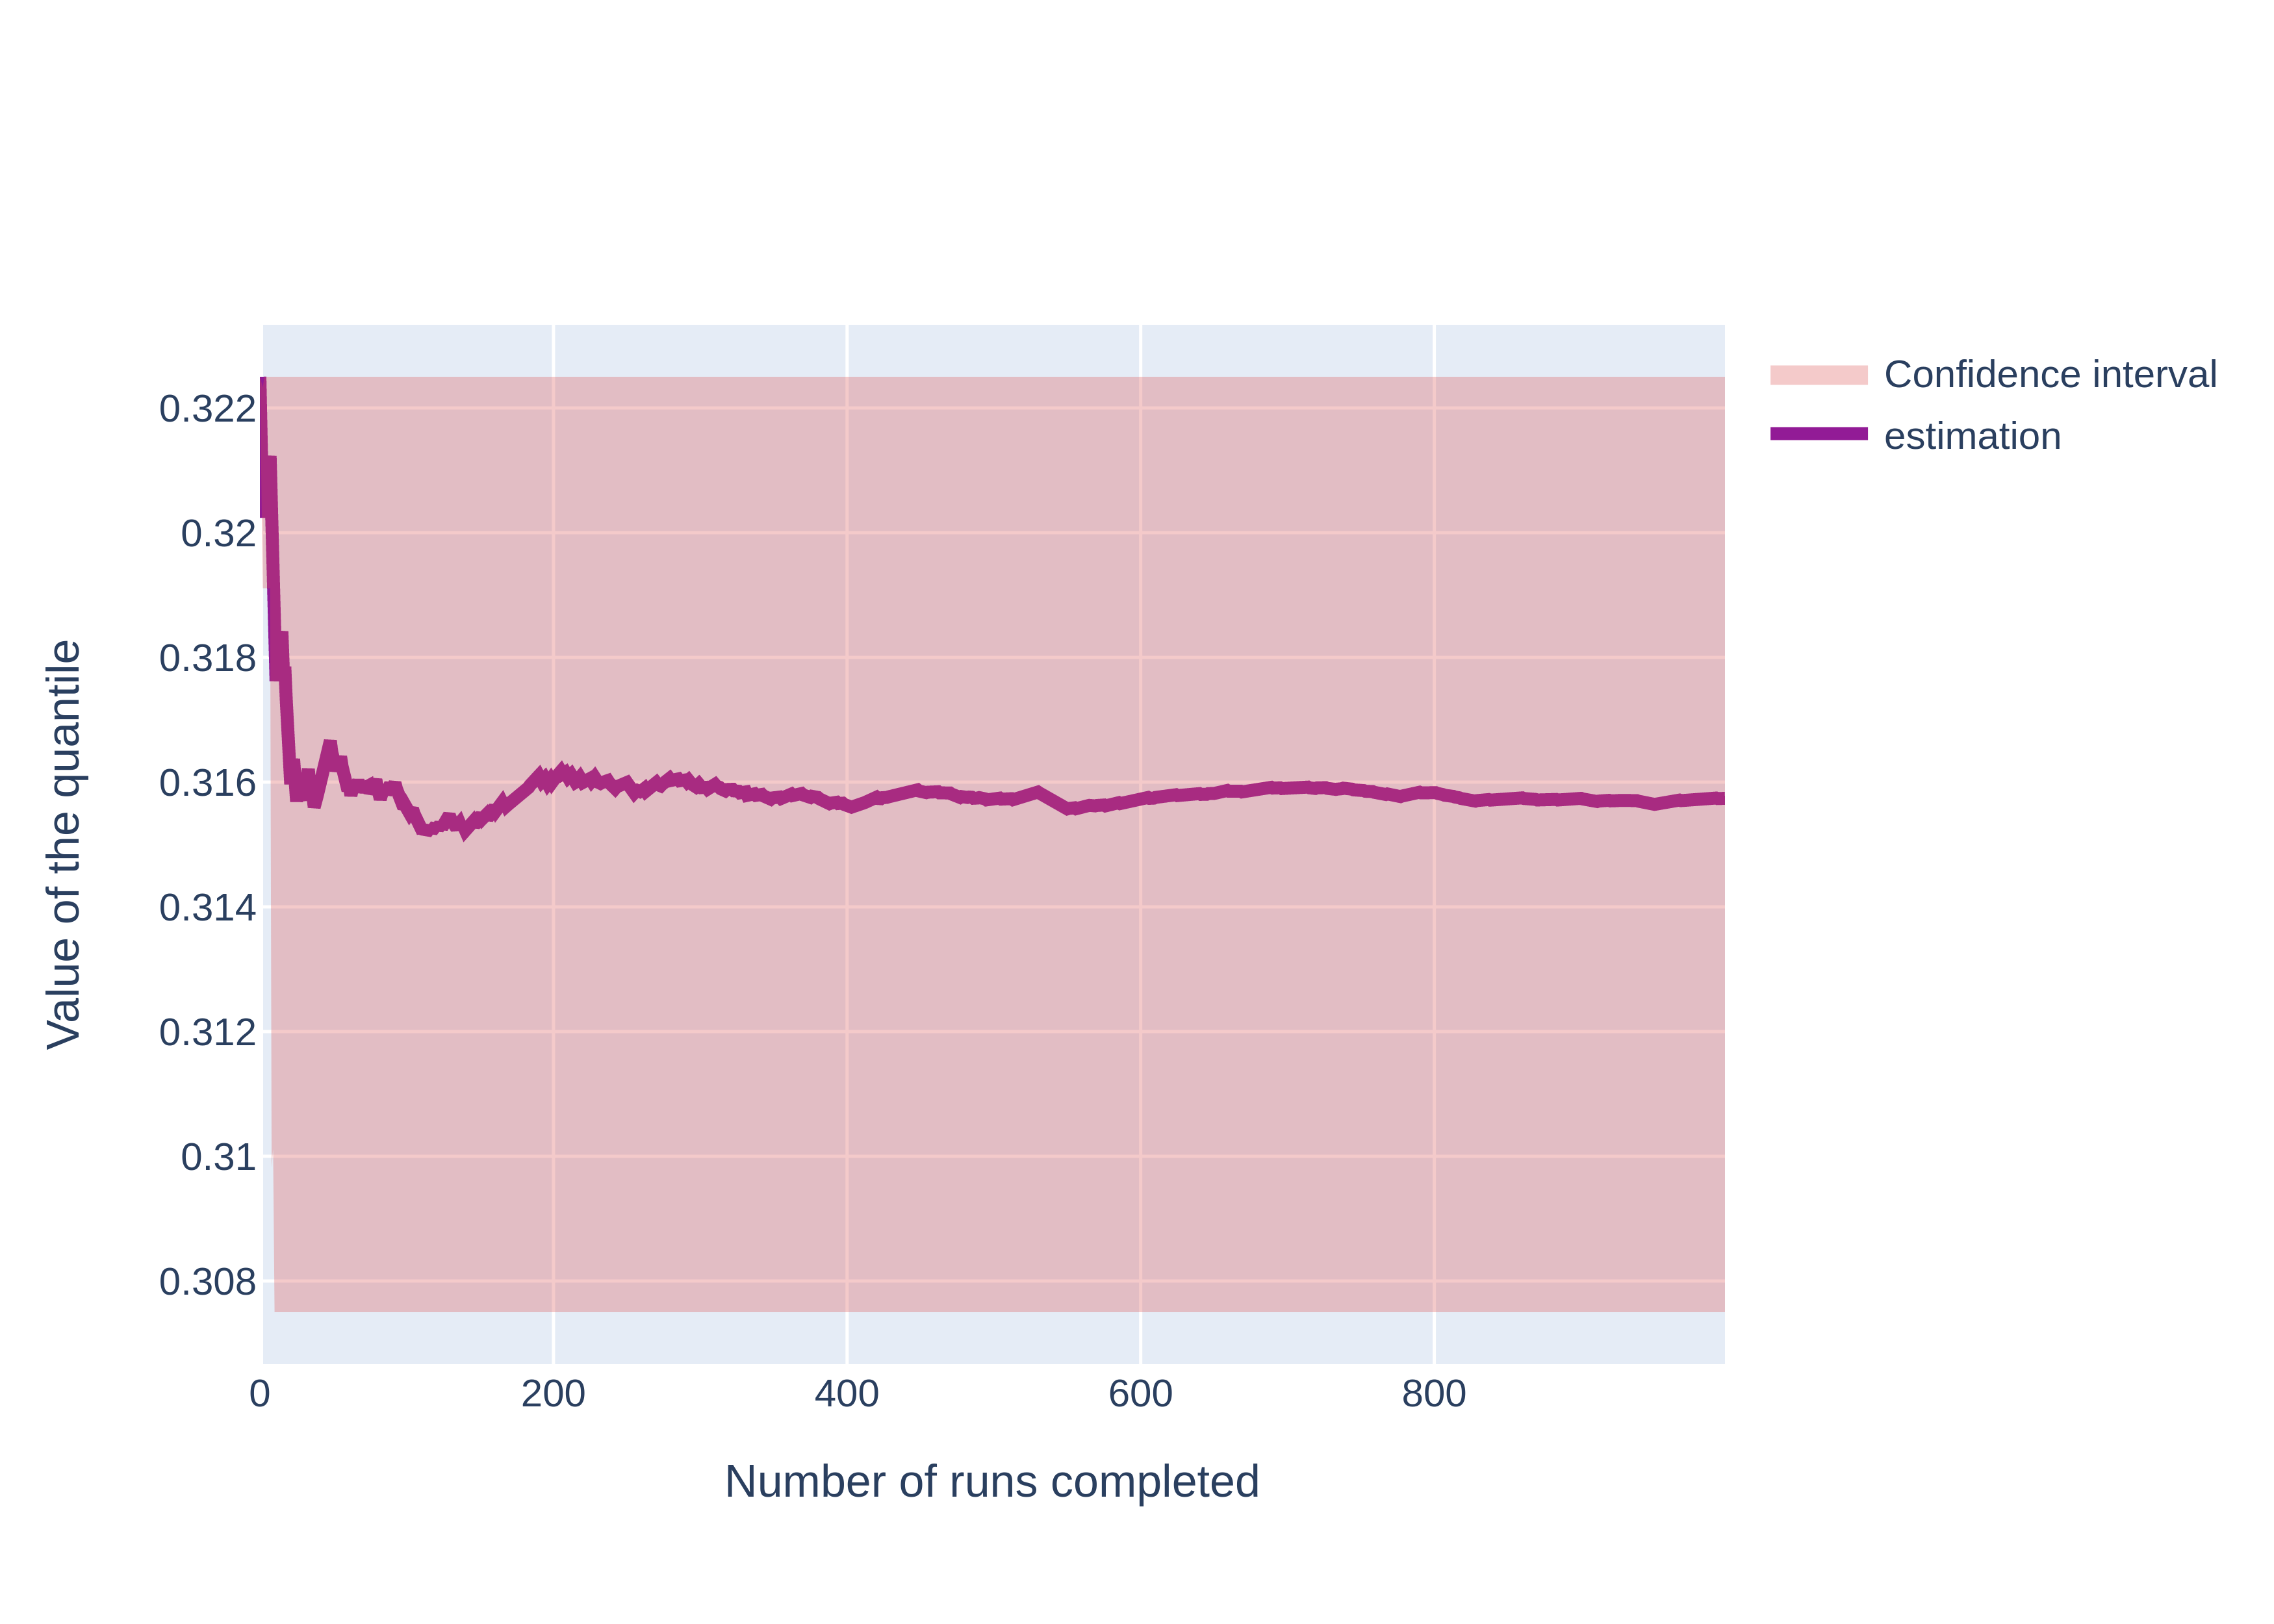
\includegraphics[width=\textwidth]{../fig/quantile4/CC1: CAM2 --> ECU2_24s.png}
        \caption{Simulation time: 24s}
        \vspace{.5cm}
    \end{subfigure}
    \begin{subfigure}{.495\textwidth}
        \centering
        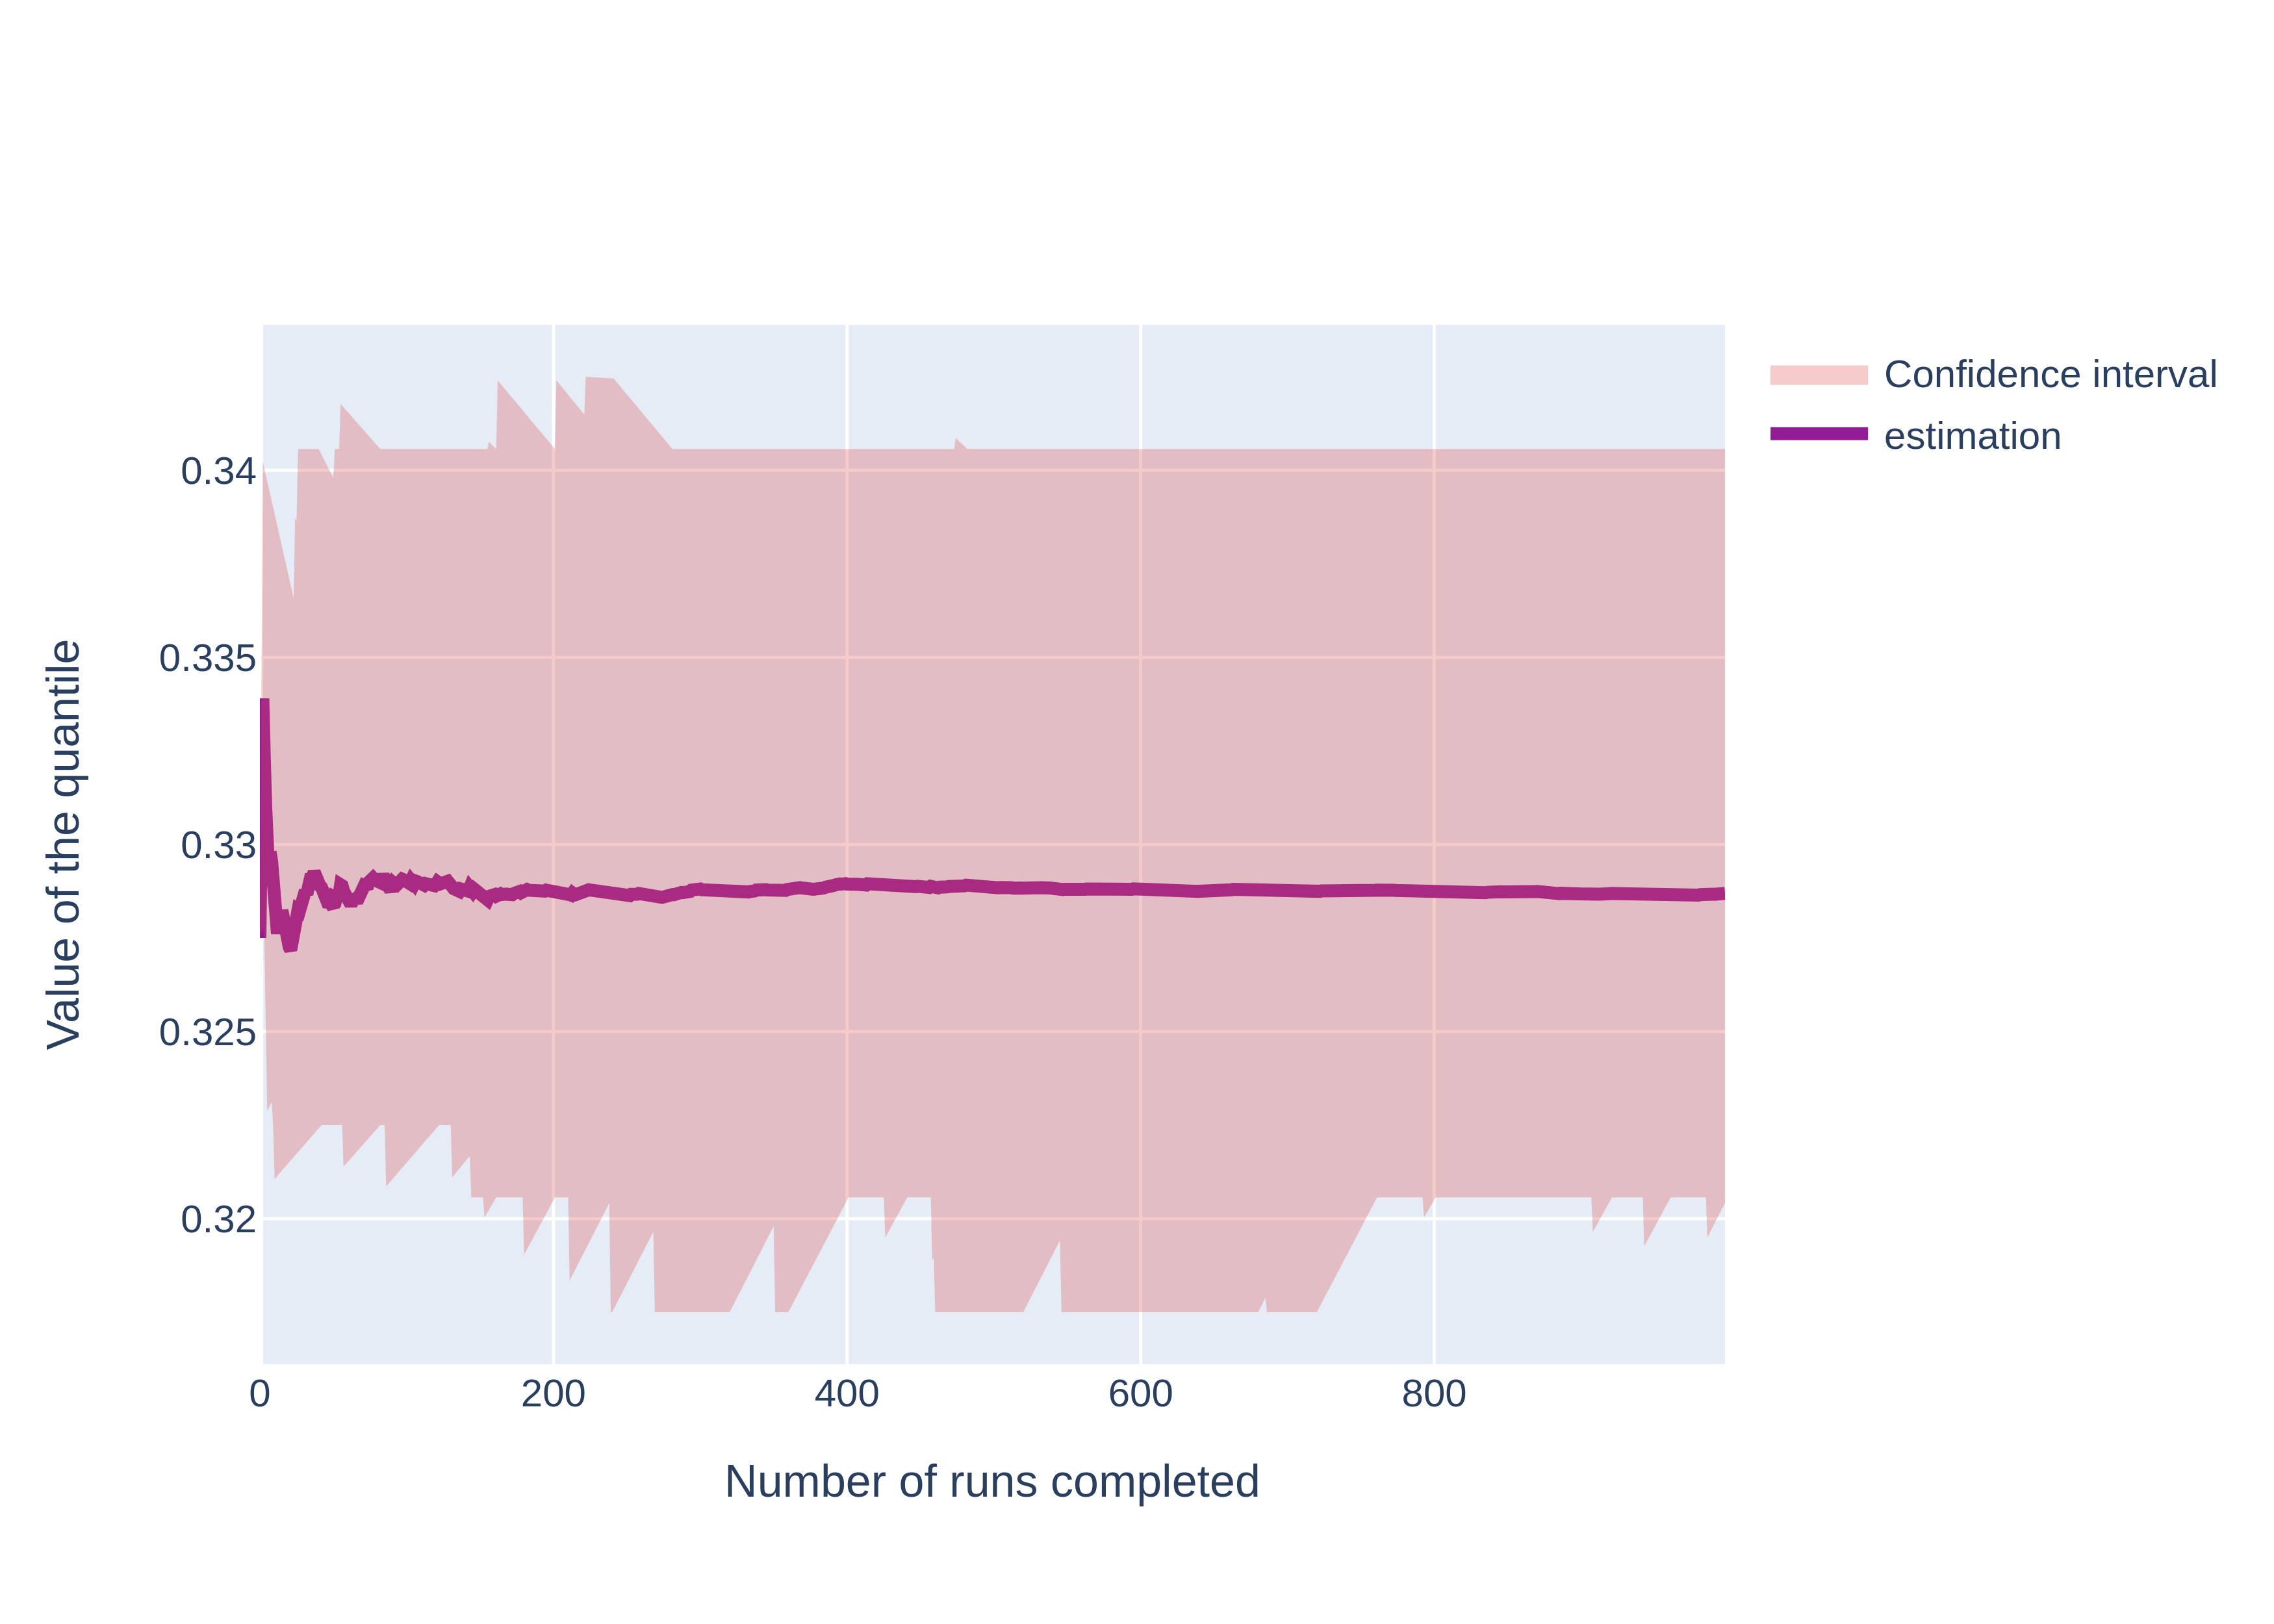
\includegraphics[width=\textwidth]{../fig/quantile4/CC1: CAM2 --> ECU2_4mn.png}
        \caption{Simulation time: 4min}
        \vspace{.5cm}
    \end{subfigure}
    \begin{subfigure}{.495\textwidth}
        \centering
        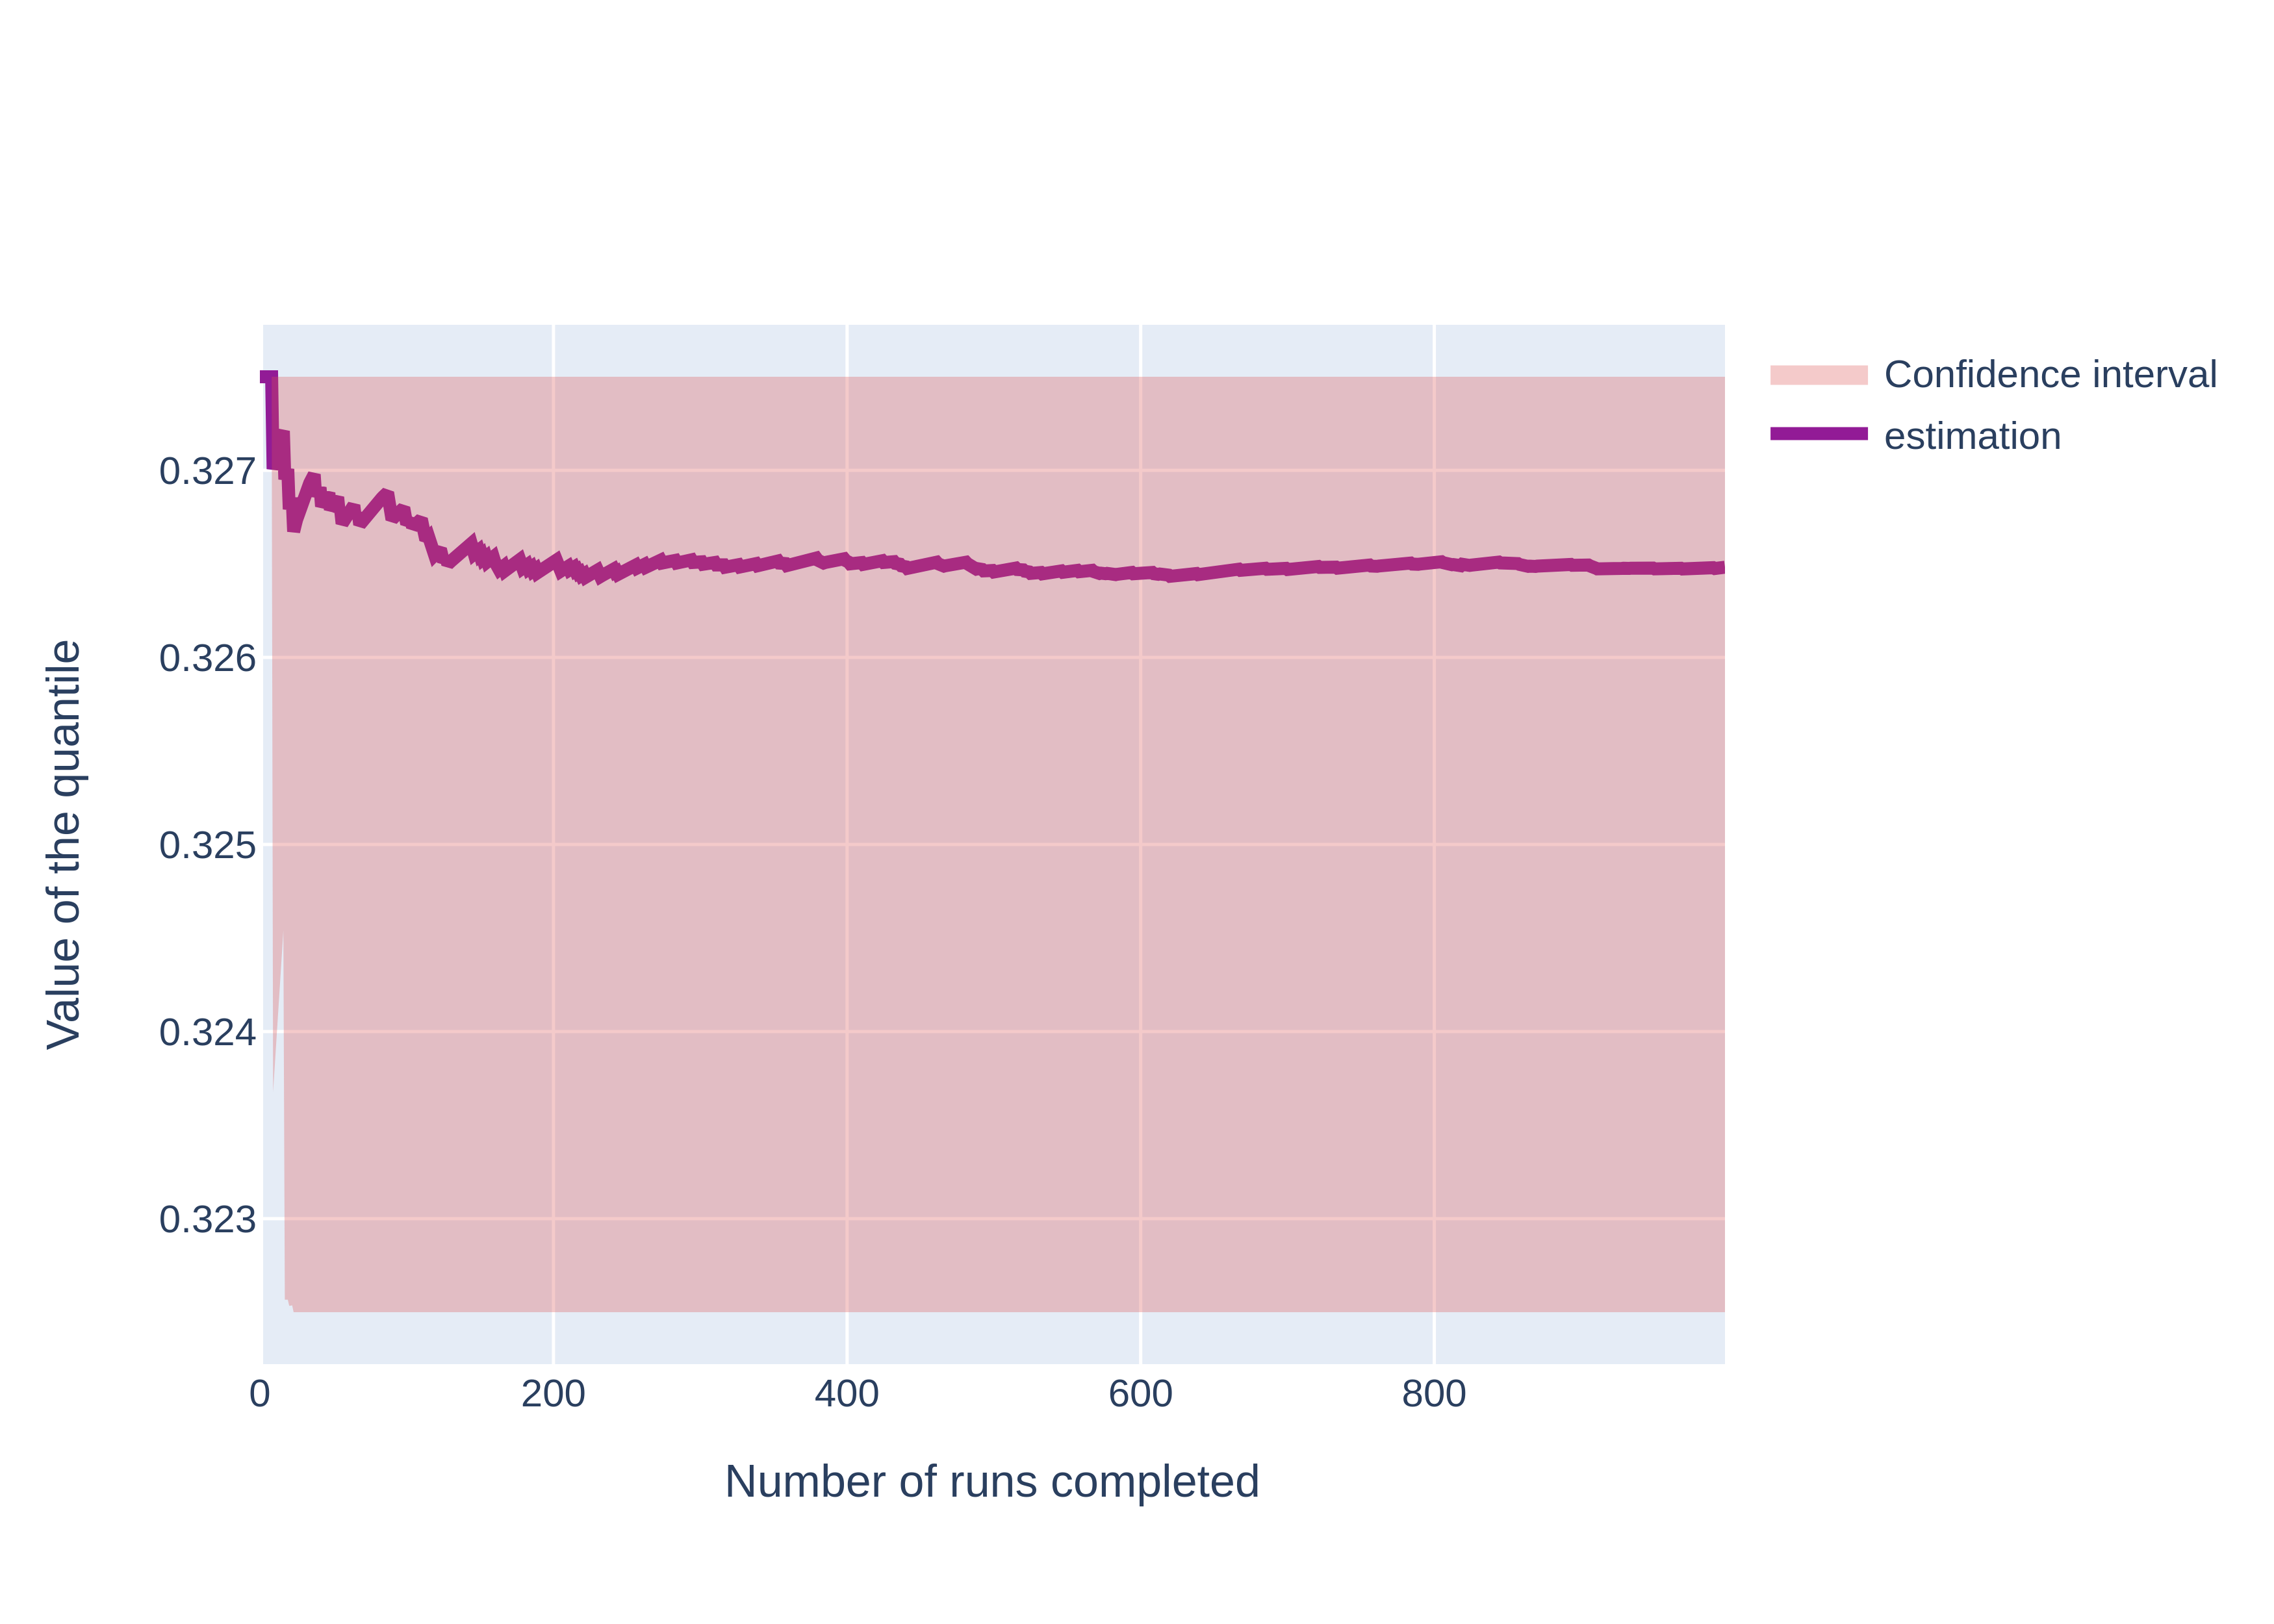
\includegraphics[width=\textwidth]{../fig/quantile4/CC1: CAM2 --> ECU2_40mn.png}
        \caption{Simulation time: 40min}
    \end{subfigure}
    \begin{subfigure}{.495\textwidth}
        \centering
        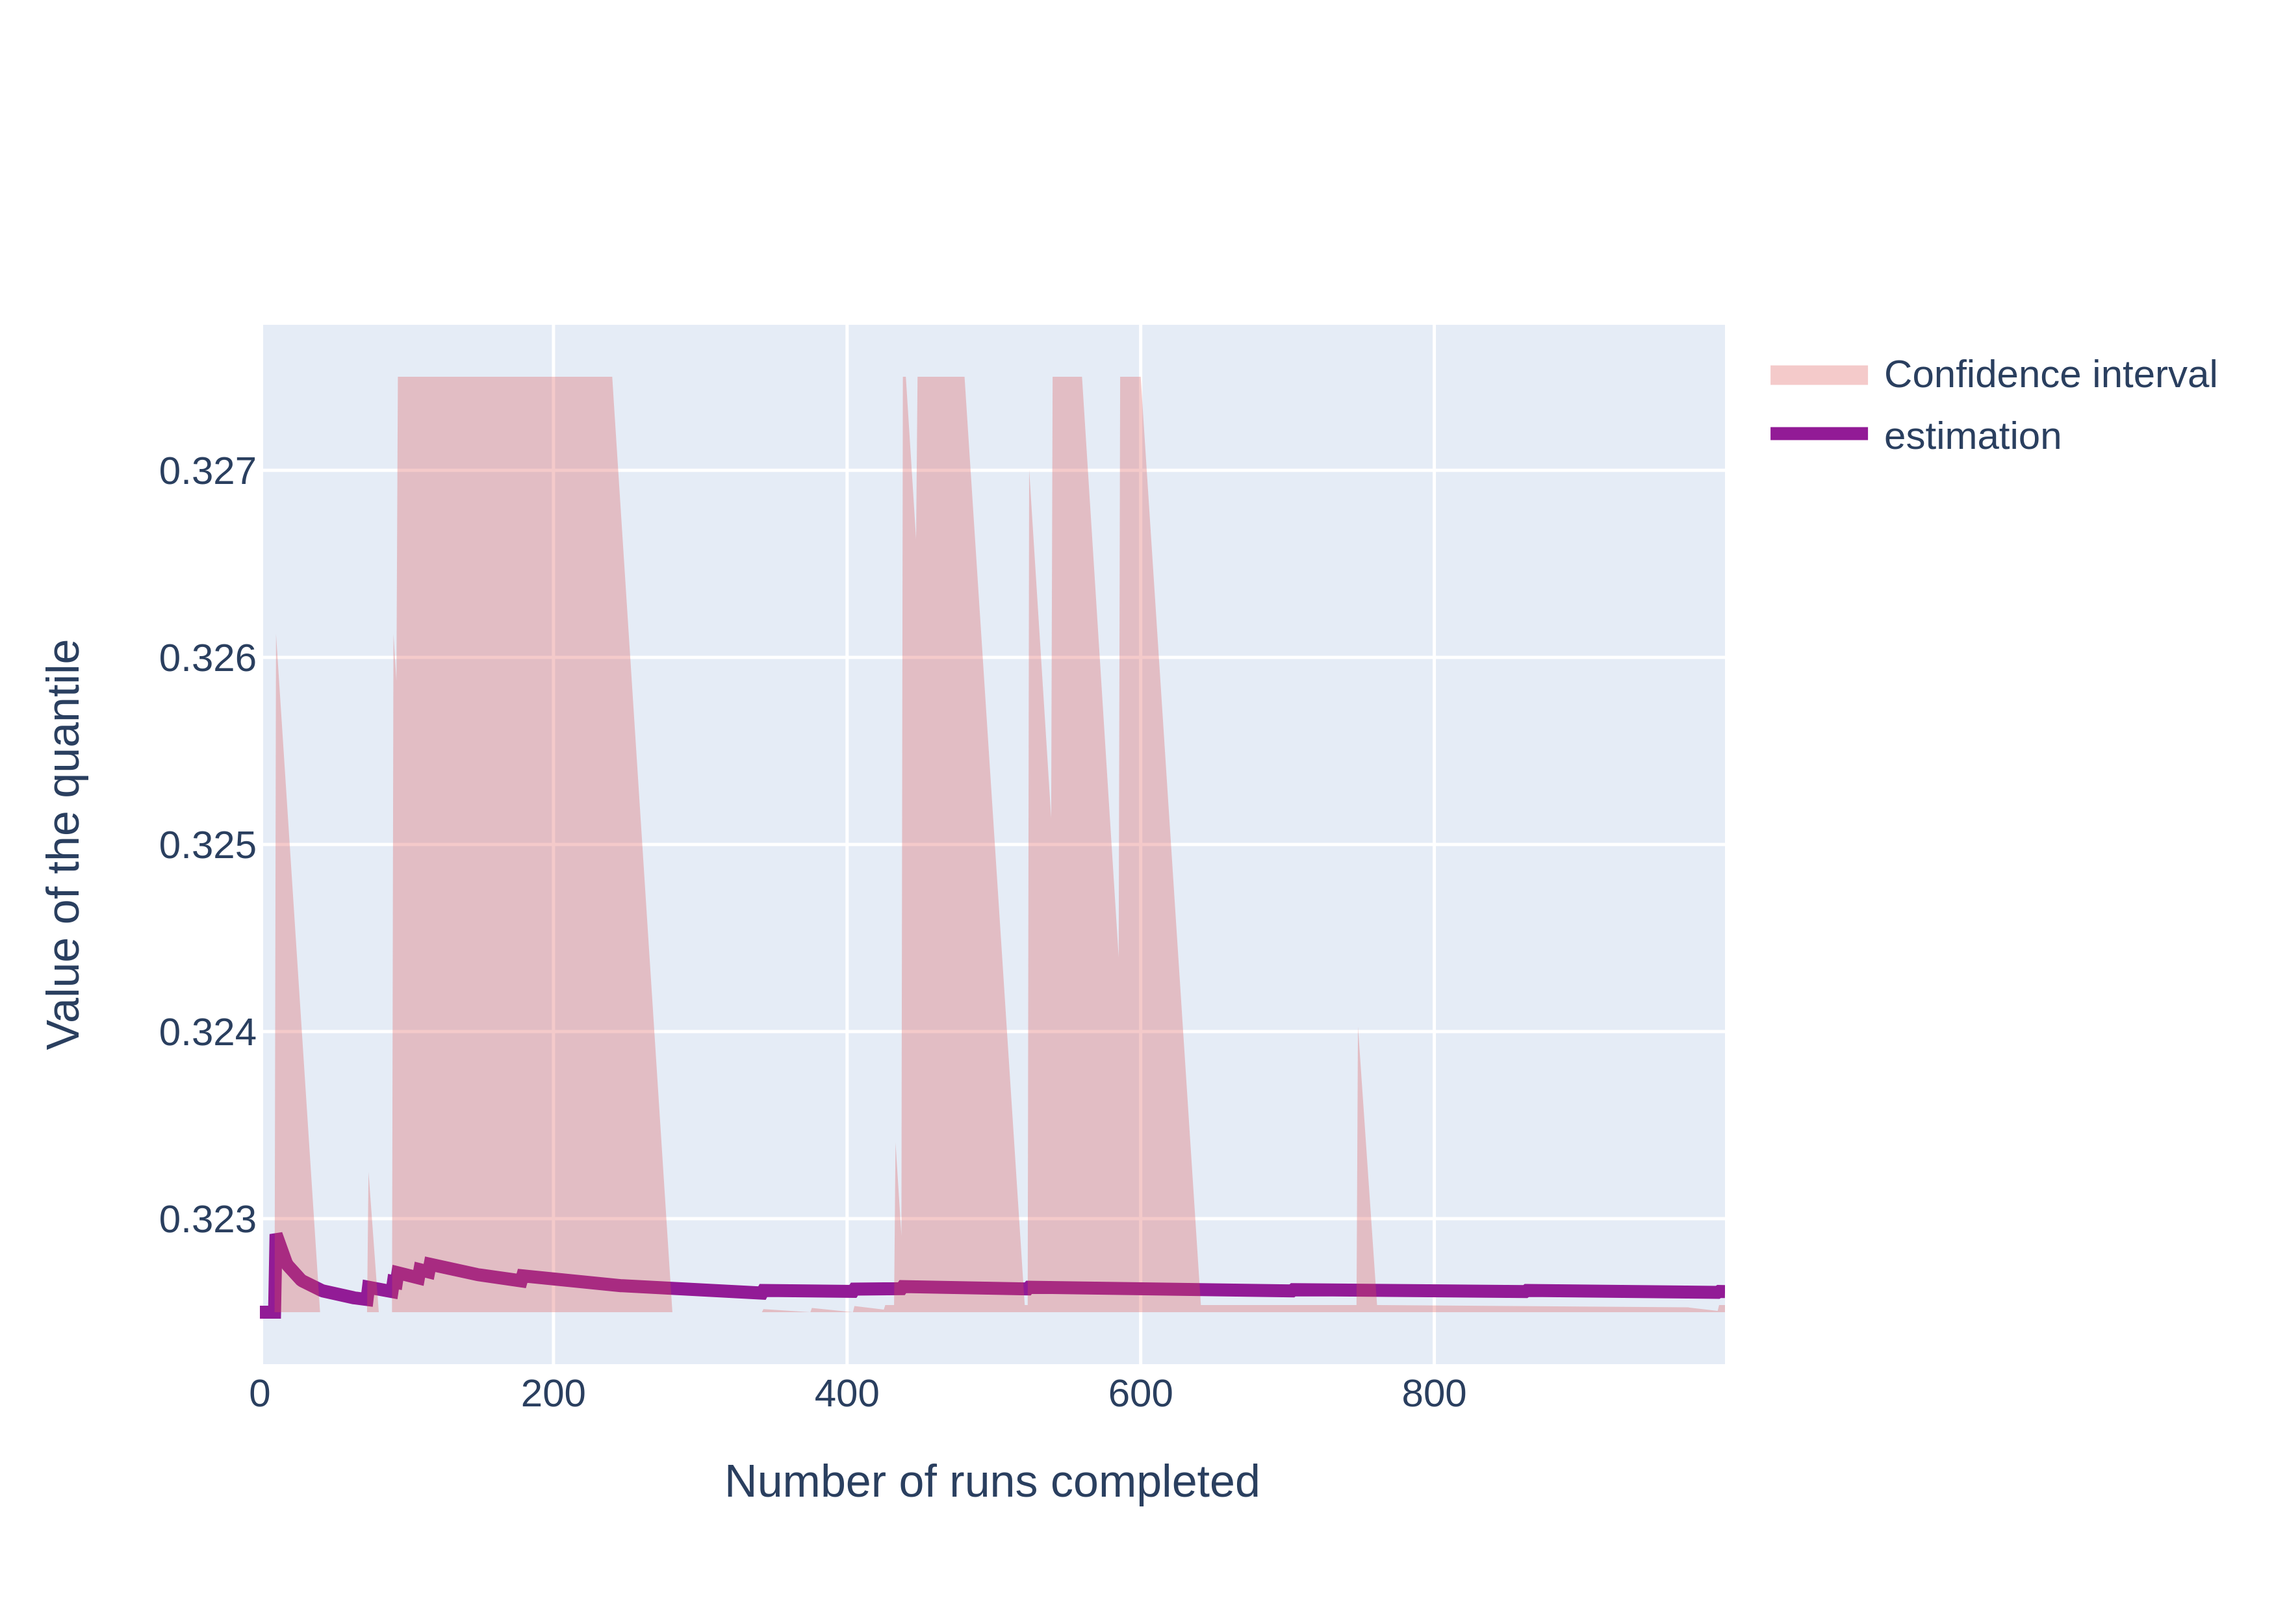
\includegraphics[width=\textwidth]{../fig/quantile4/CC1: CAM2 --> ECU2_400mn.png}
        \caption{Simulation time: 400min}
    \end{subfigure}
    \caption{CC1: CAM2 - ECU2 $q_4$ after multiple simulation times}
\end{figure}

\subsubsection{Quantile 5}
\begin{figure}[H]
    \centering
    \begin{subfigure}{.495\textwidth}
        \centering
        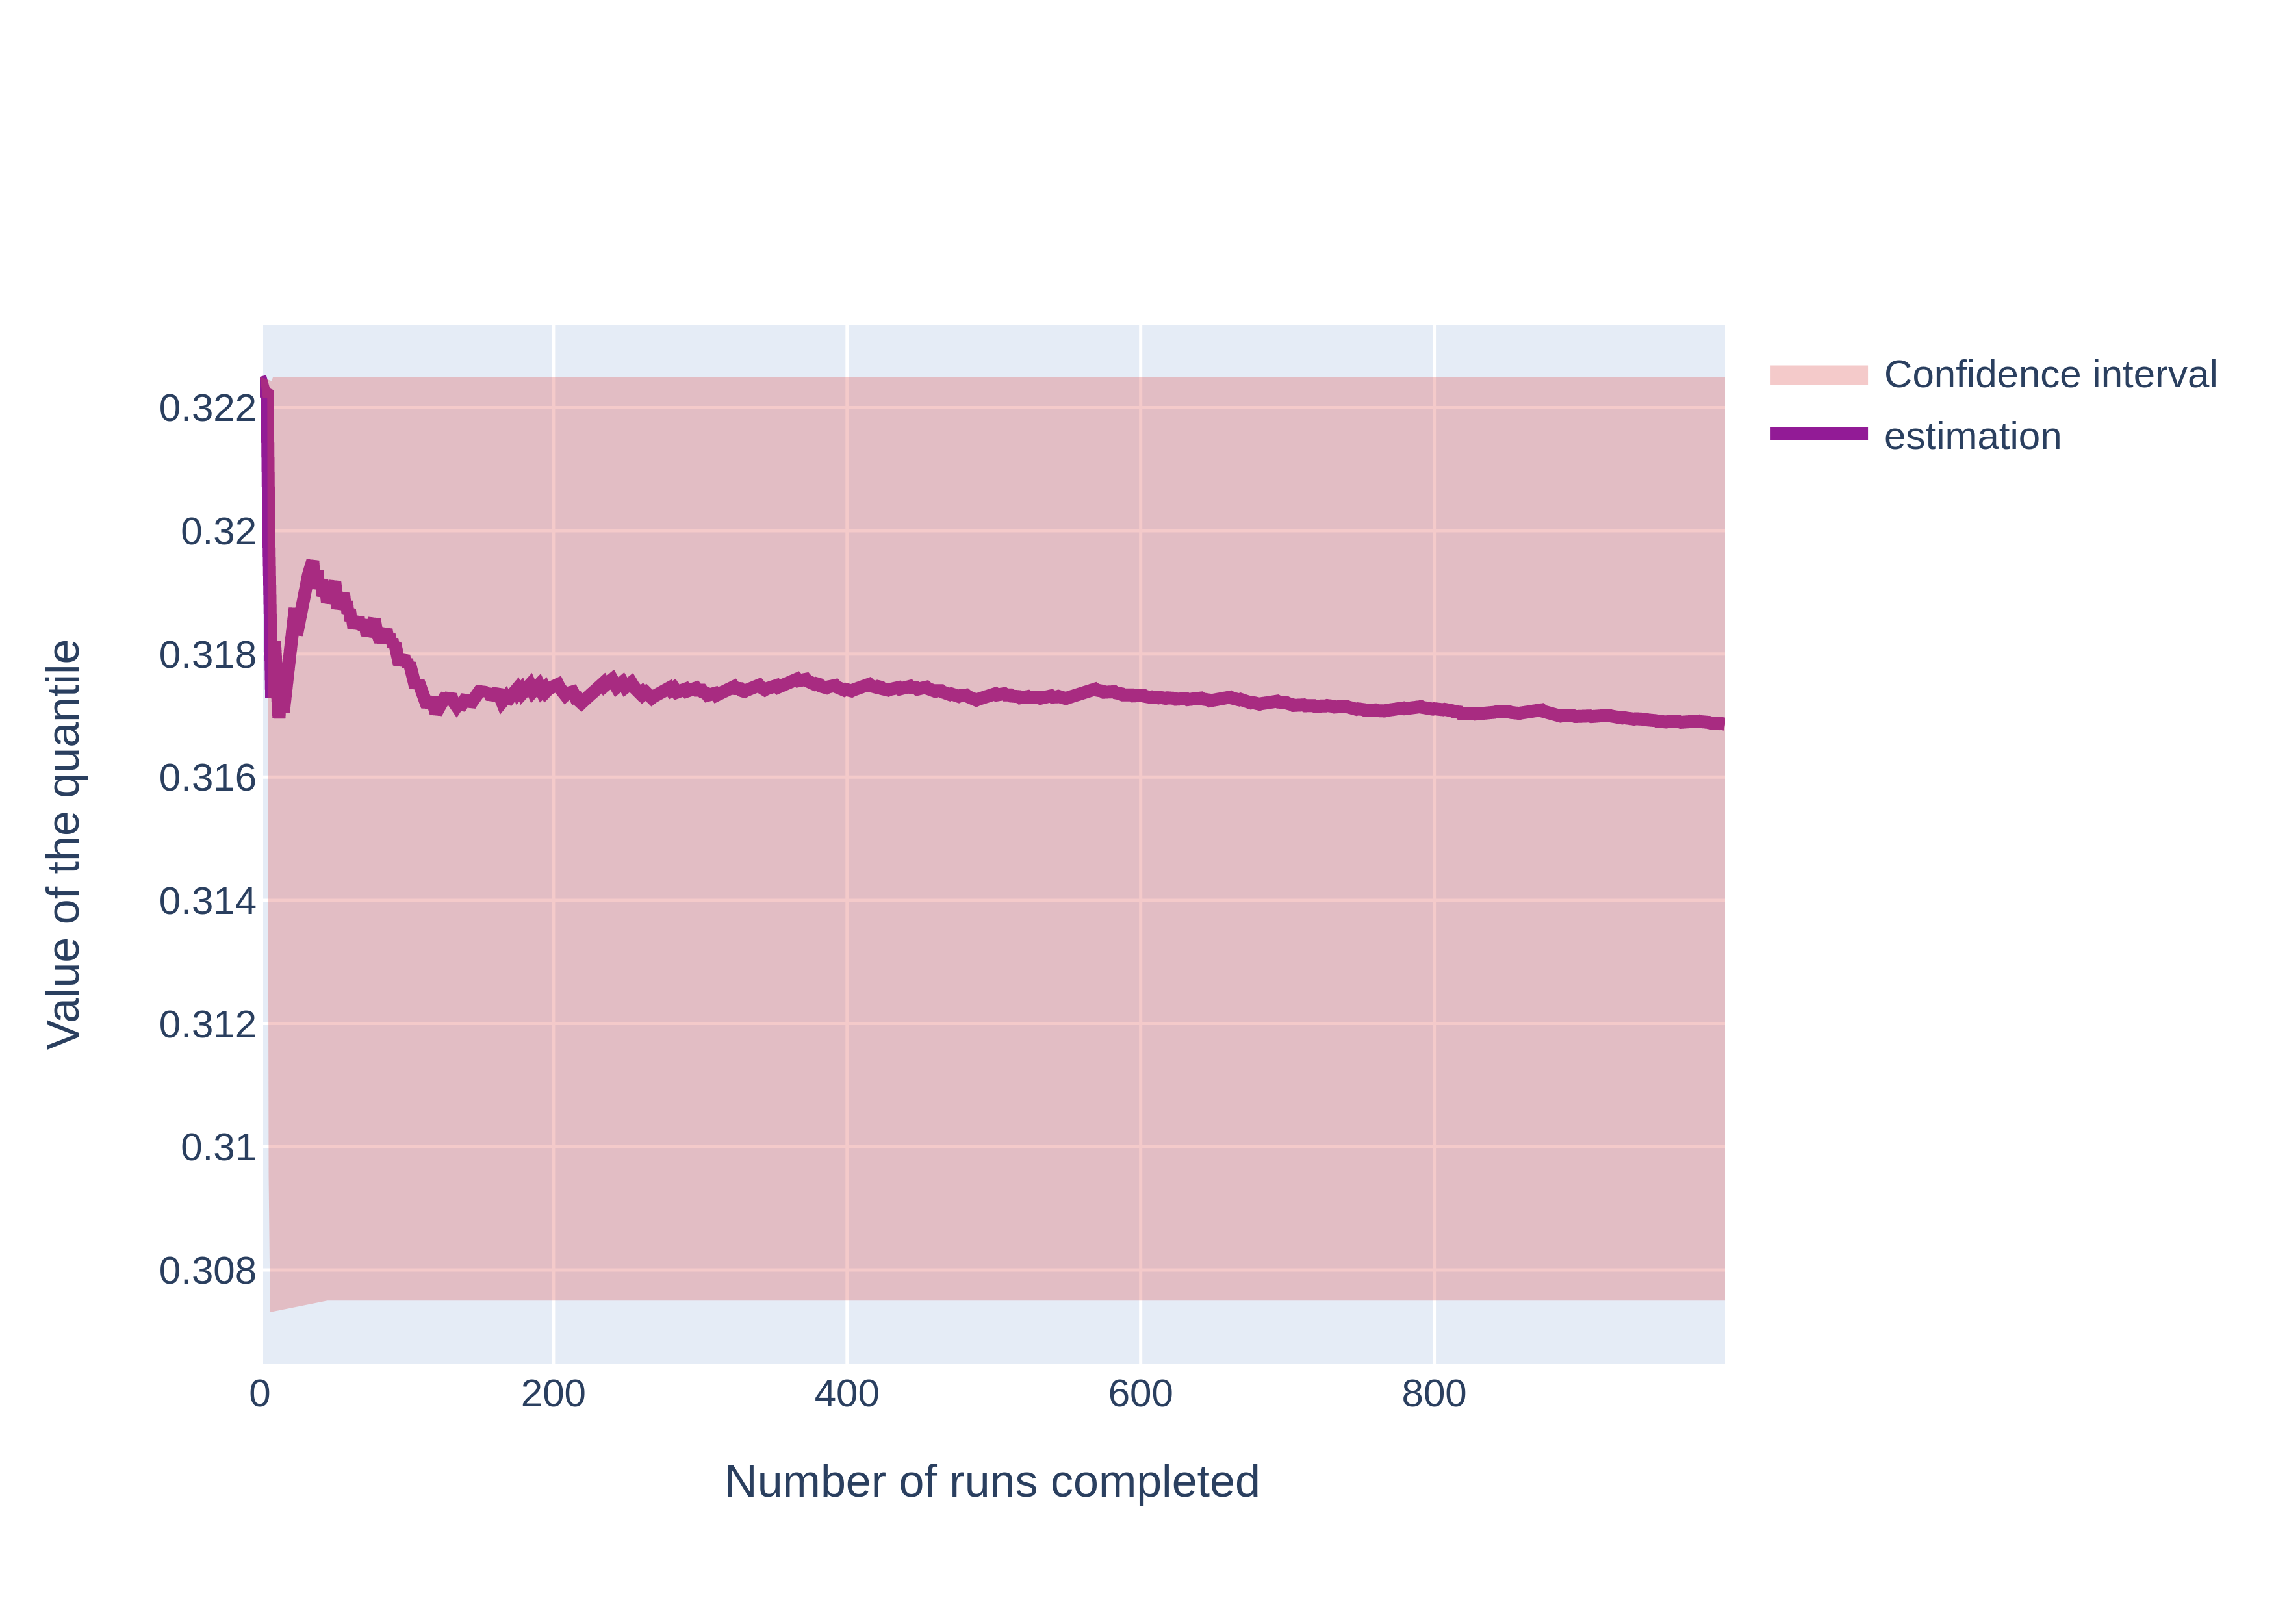
\includegraphics[width=\textwidth]{../fig/quantile5/CC1: CAM2 --> ECU2_24s.png}
        \caption{Simulation time: 24s}
        \vspace{.5cm}
    \end{subfigure}
    \begin{subfigure}{.495\textwidth}
        \centering
        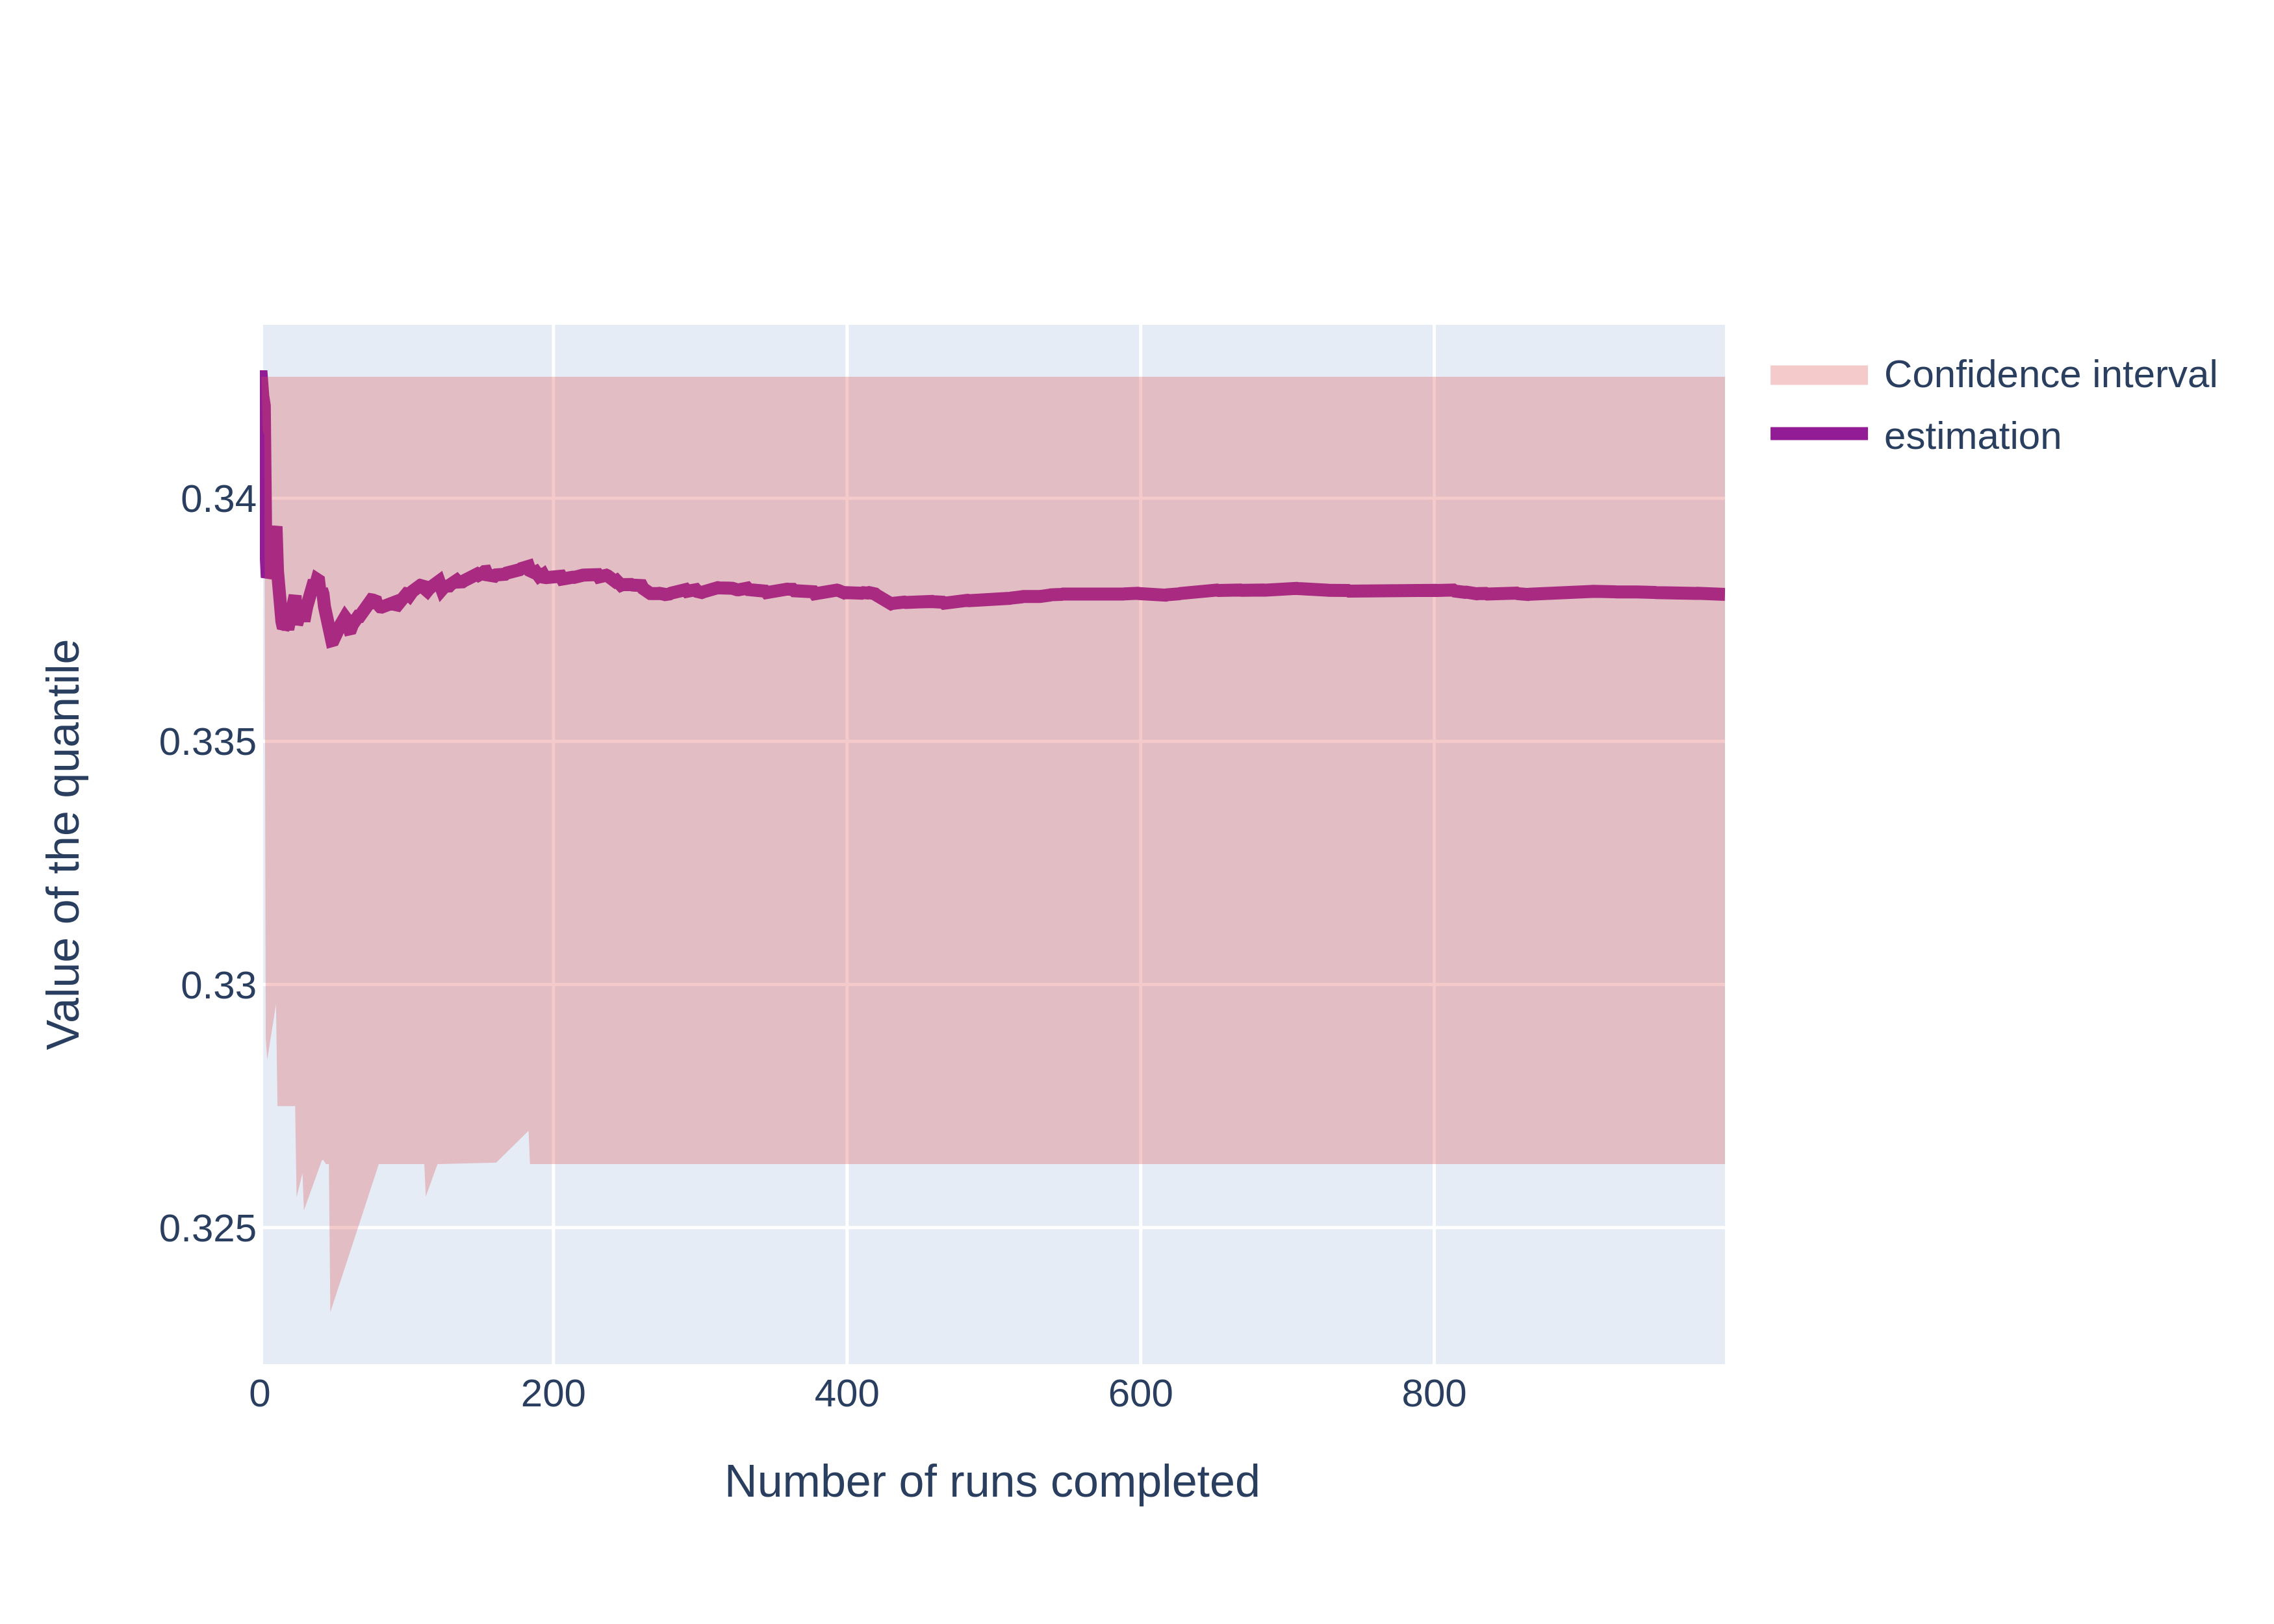
\includegraphics[width=\textwidth]{../fig/quantile5/CC1: CAM2 --> ECU2_4mn.png}
        \caption{Simulation time: 4min}
        \vspace{.5cm}
    \end{subfigure}
    \begin{subfigure}{.495\textwidth}
        \centering
        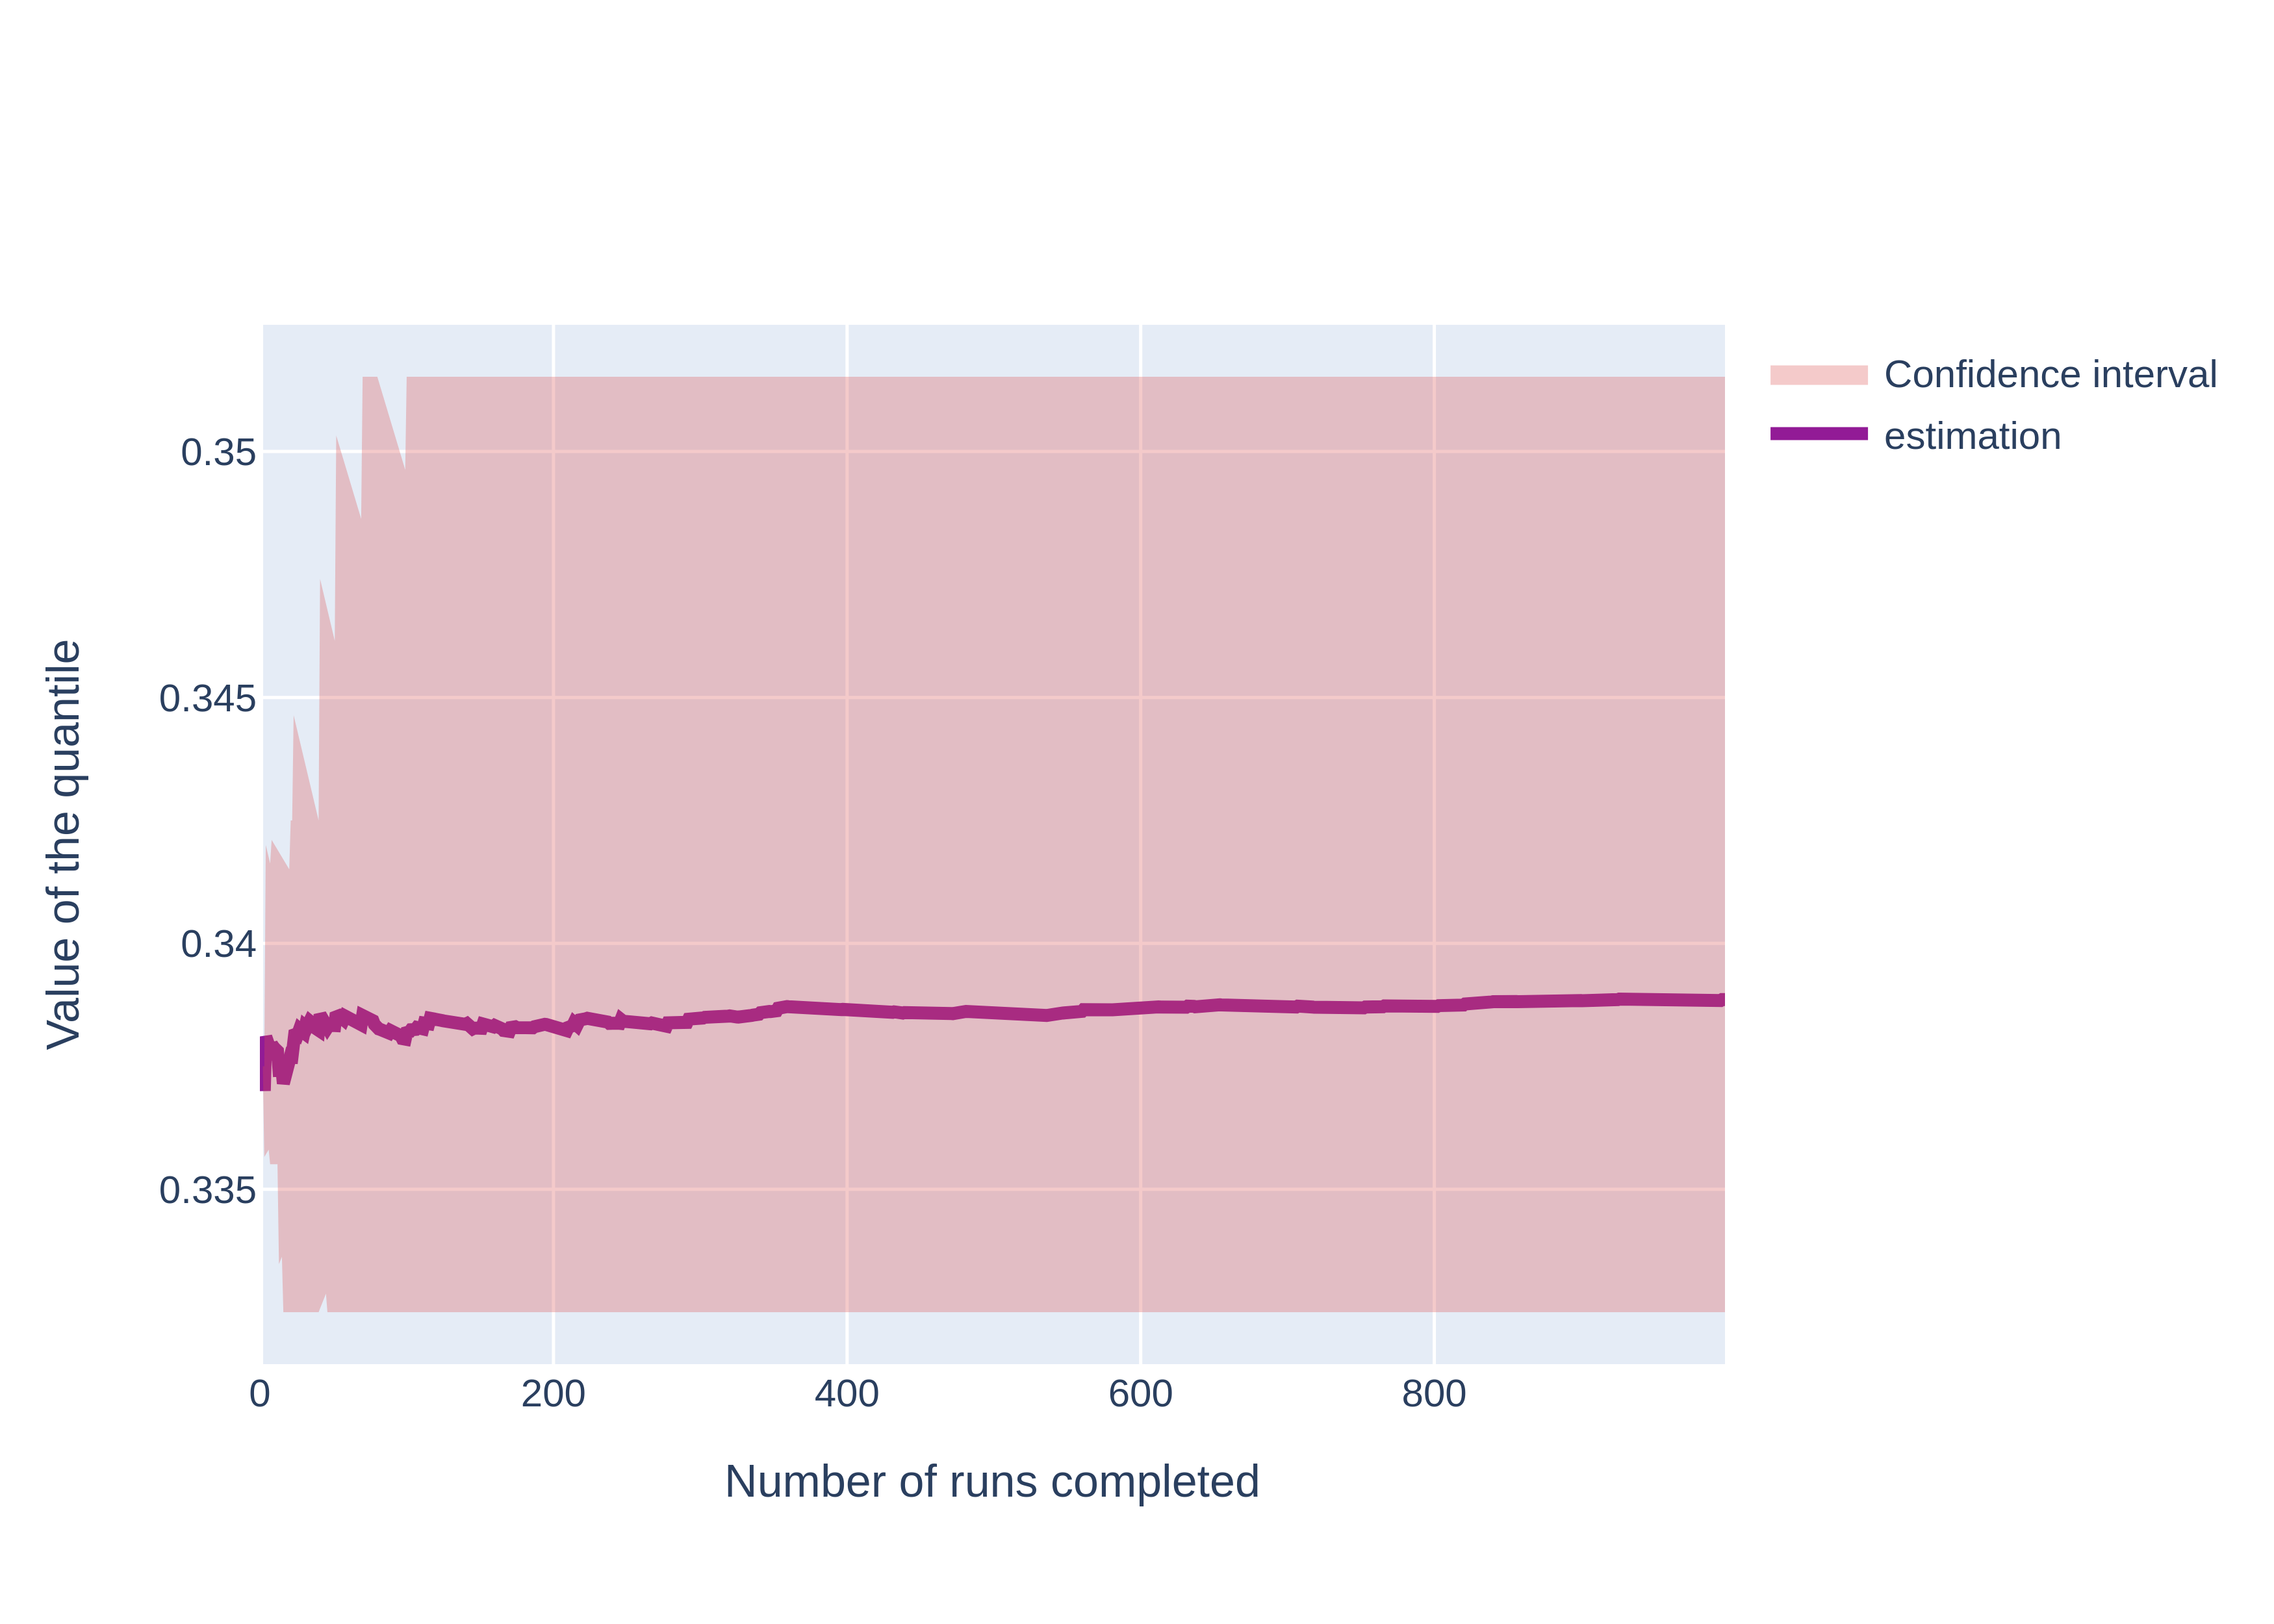
\includegraphics[width=\textwidth]{../fig/quantile5/CC1: CAM2 --> ECU2_40mn.png}
        \caption{Simulation time: 40min}
    \end{subfigure}
    \begin{subfigure}{.495\textwidth}
        \centering
        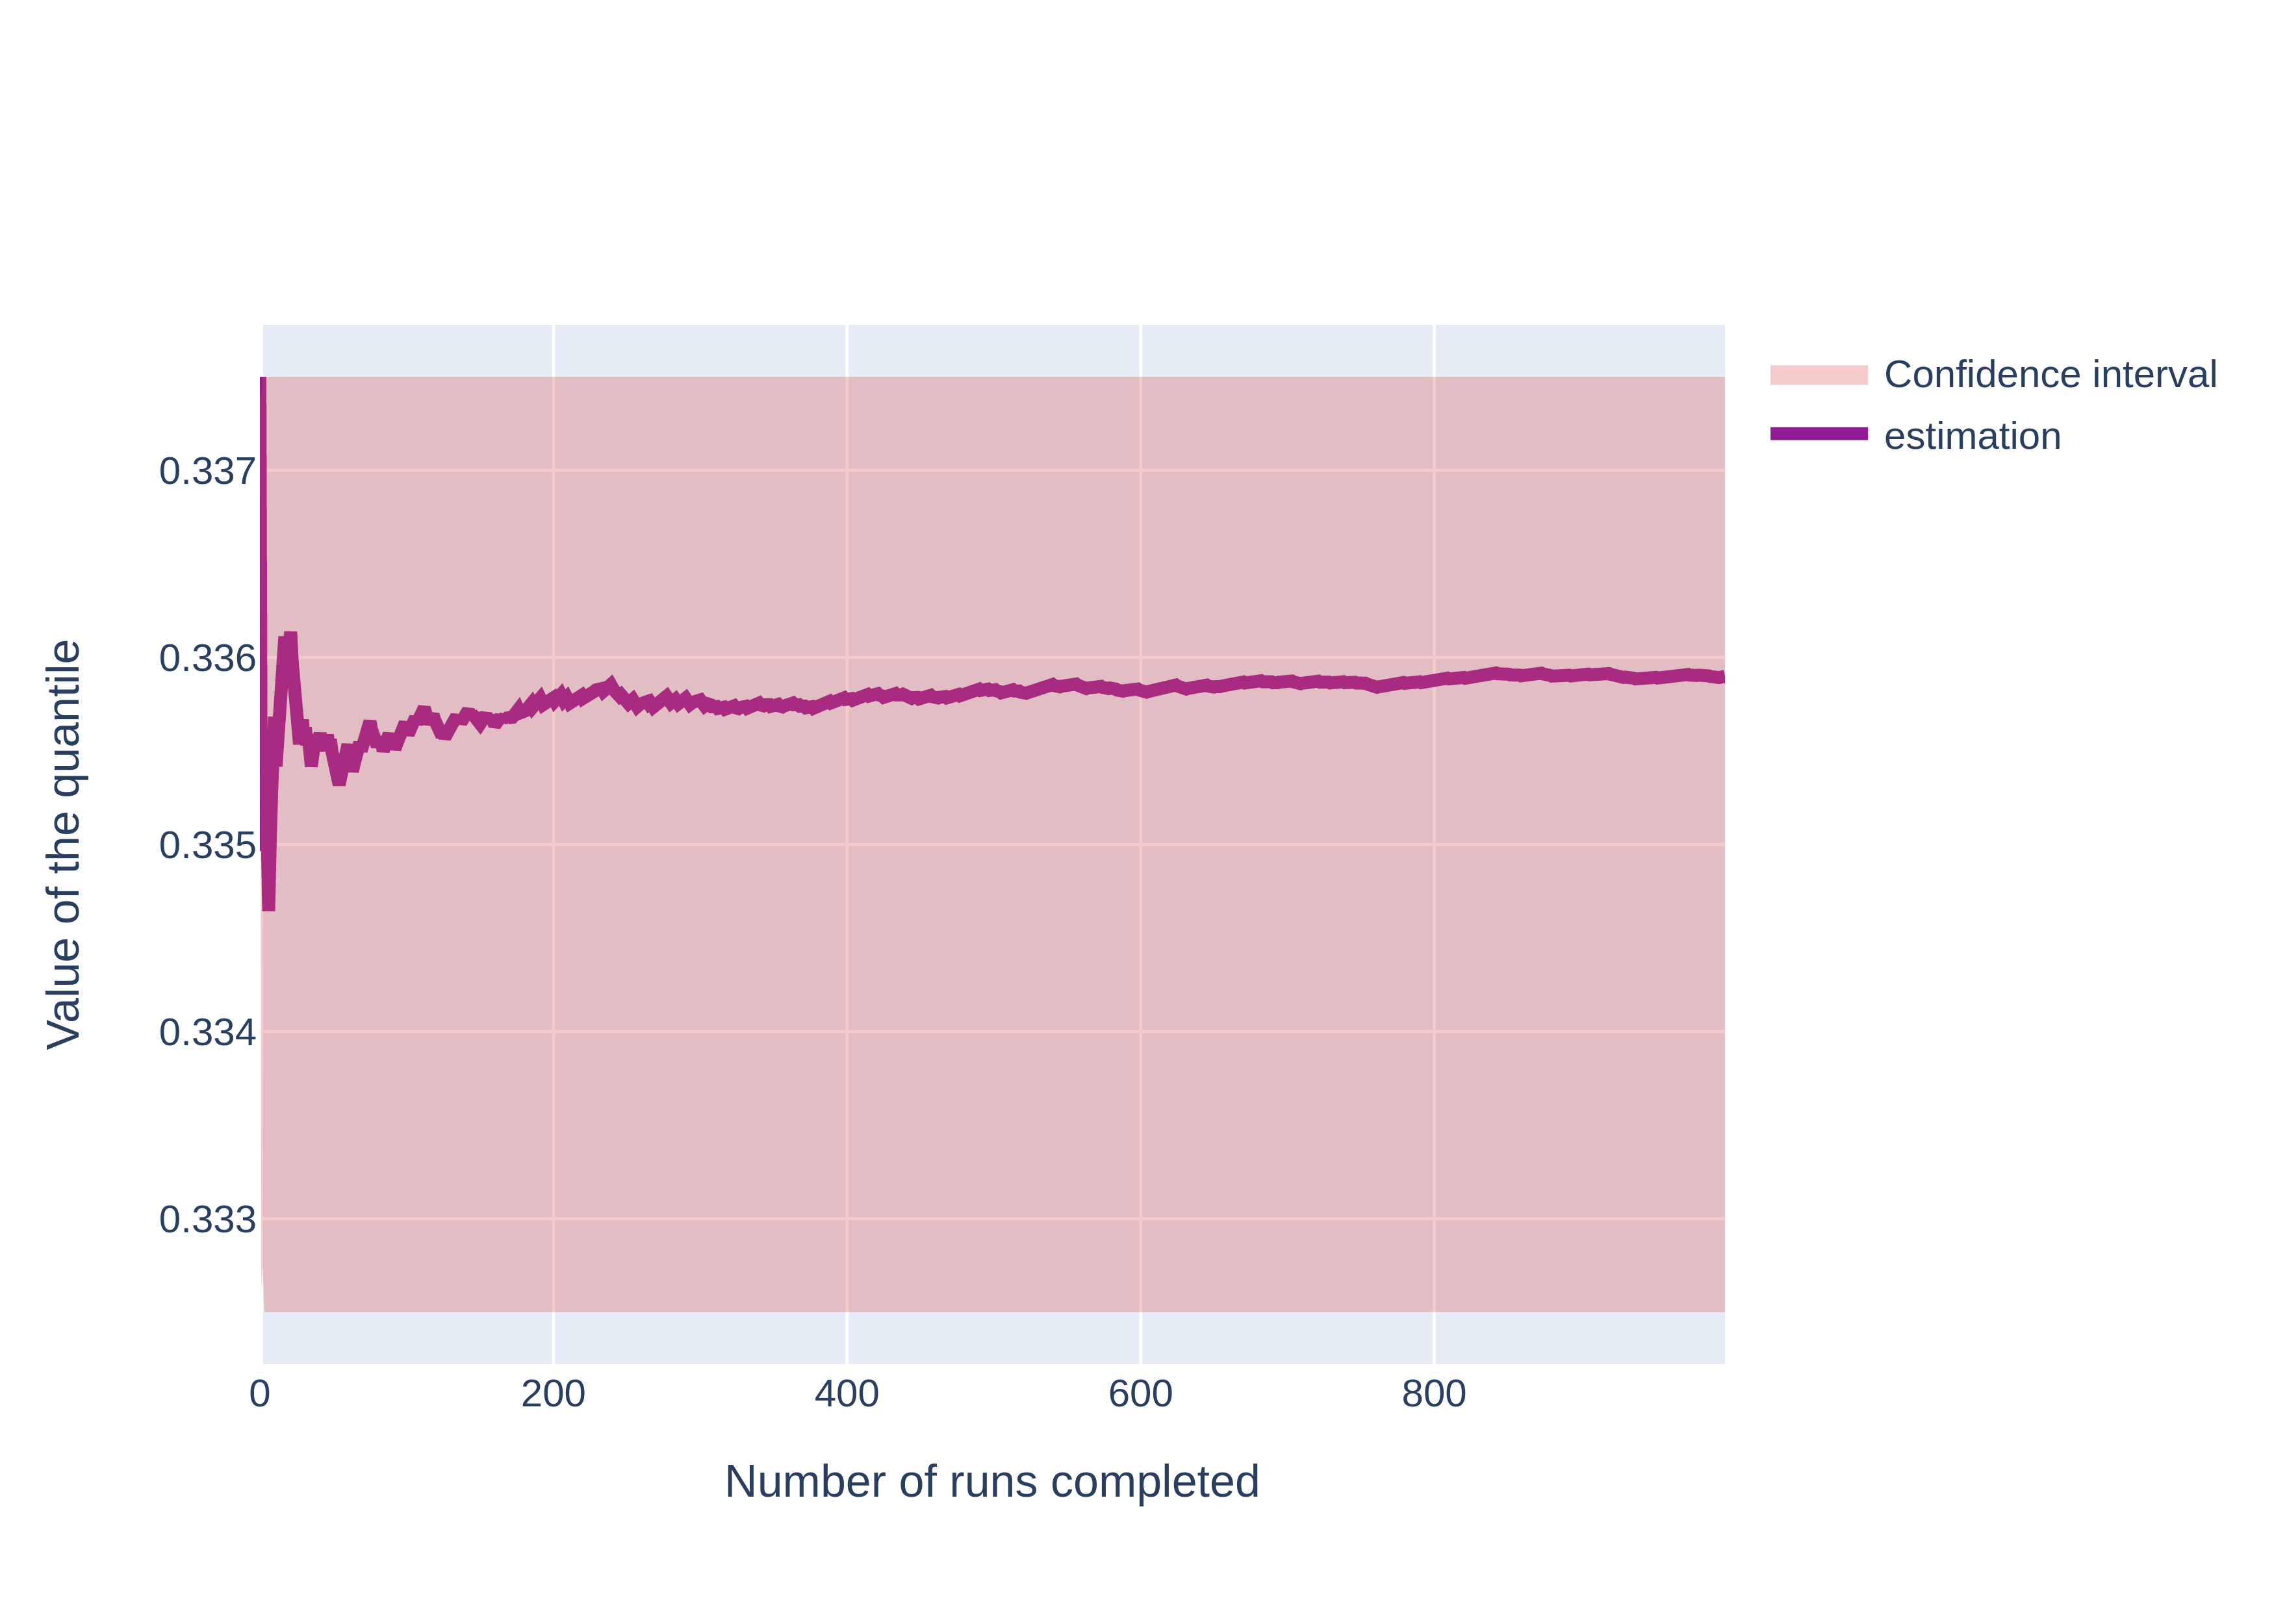
\includegraphics[width=\textwidth]{../fig/quantile5/CC1: CAM2 --> ECU2_400mn.png}
        \caption{Simulation time: 400min}
    \end{subfigure}
    \caption{CC1: CAM2 - ECU2 $q_5$ after multiple simulation times}
\end{figure}



\subsection{TFTP4 DAT}
\subsubsection{Data}

\begin{figure}[H]
    \centering
    \begin{subfigure}{.495\textwidth}
        \centering
        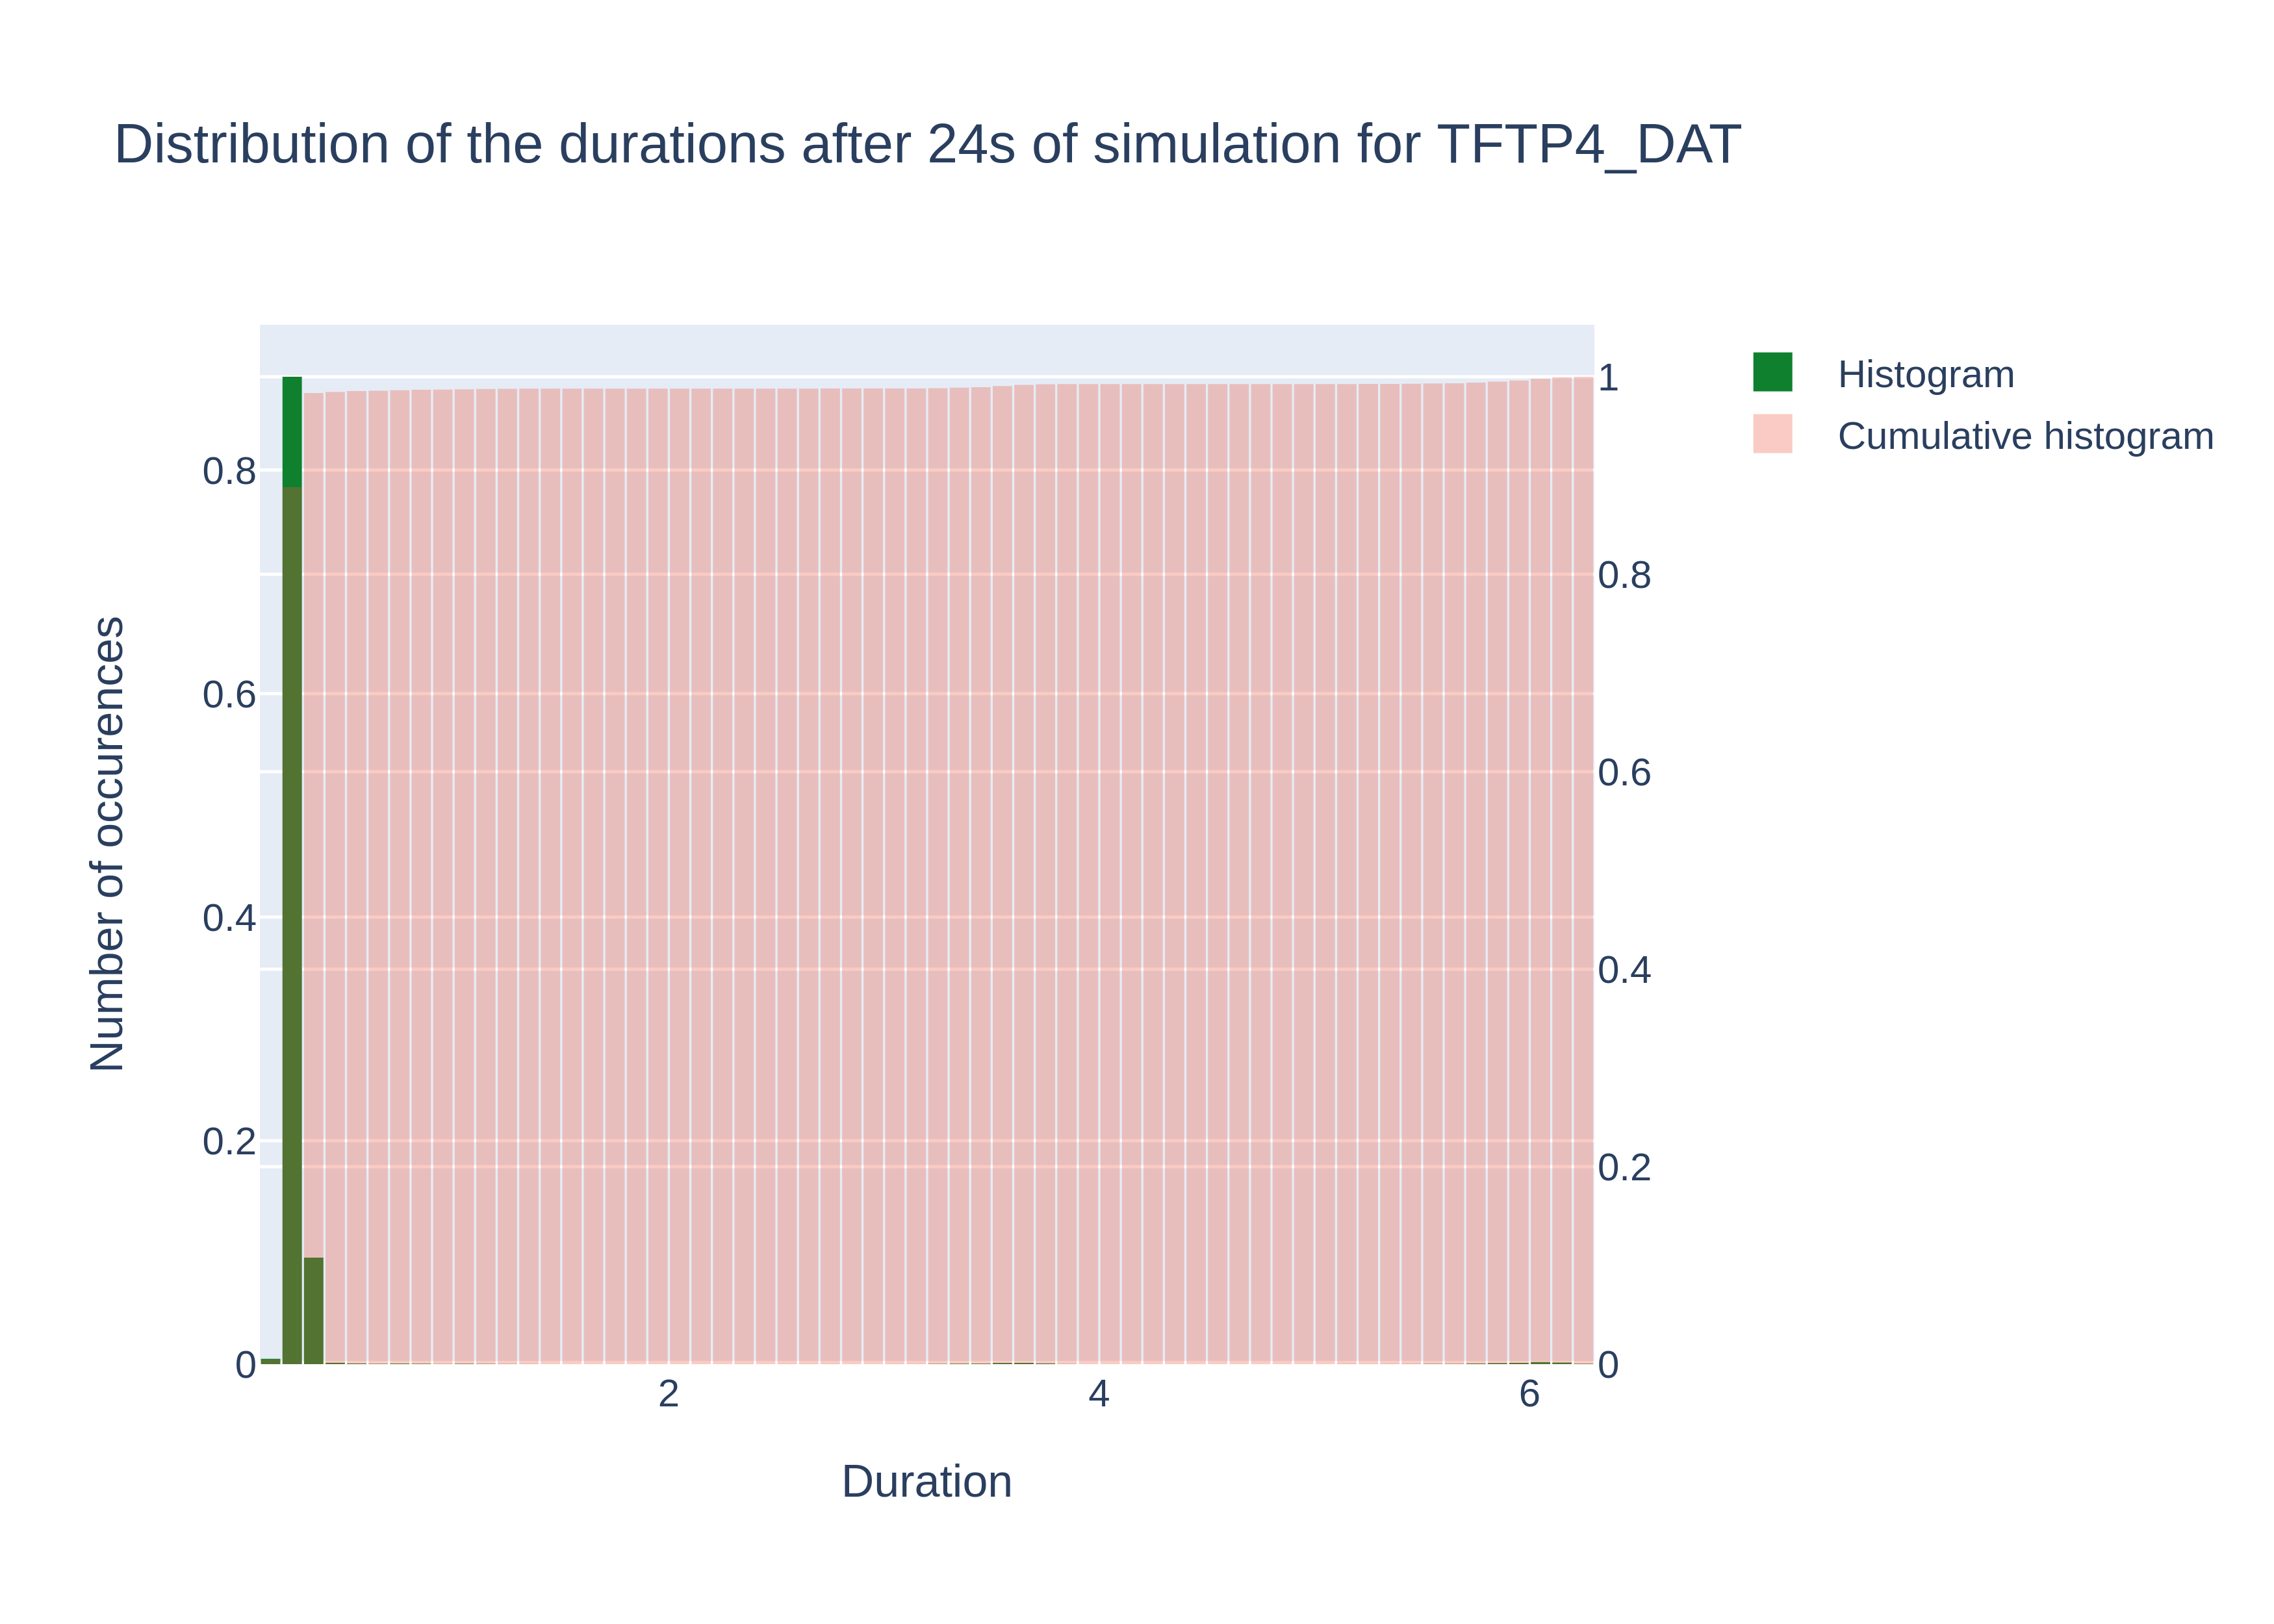
\includegraphics[width=\textwidth]{../fig/data/TFTP4_DAT_24s.png}
        \caption{Simulation time: 24s}
        \vspace{.5cm}
    \end{subfigure}
    \begin{subfigure}{.495\textwidth}
        \centering
        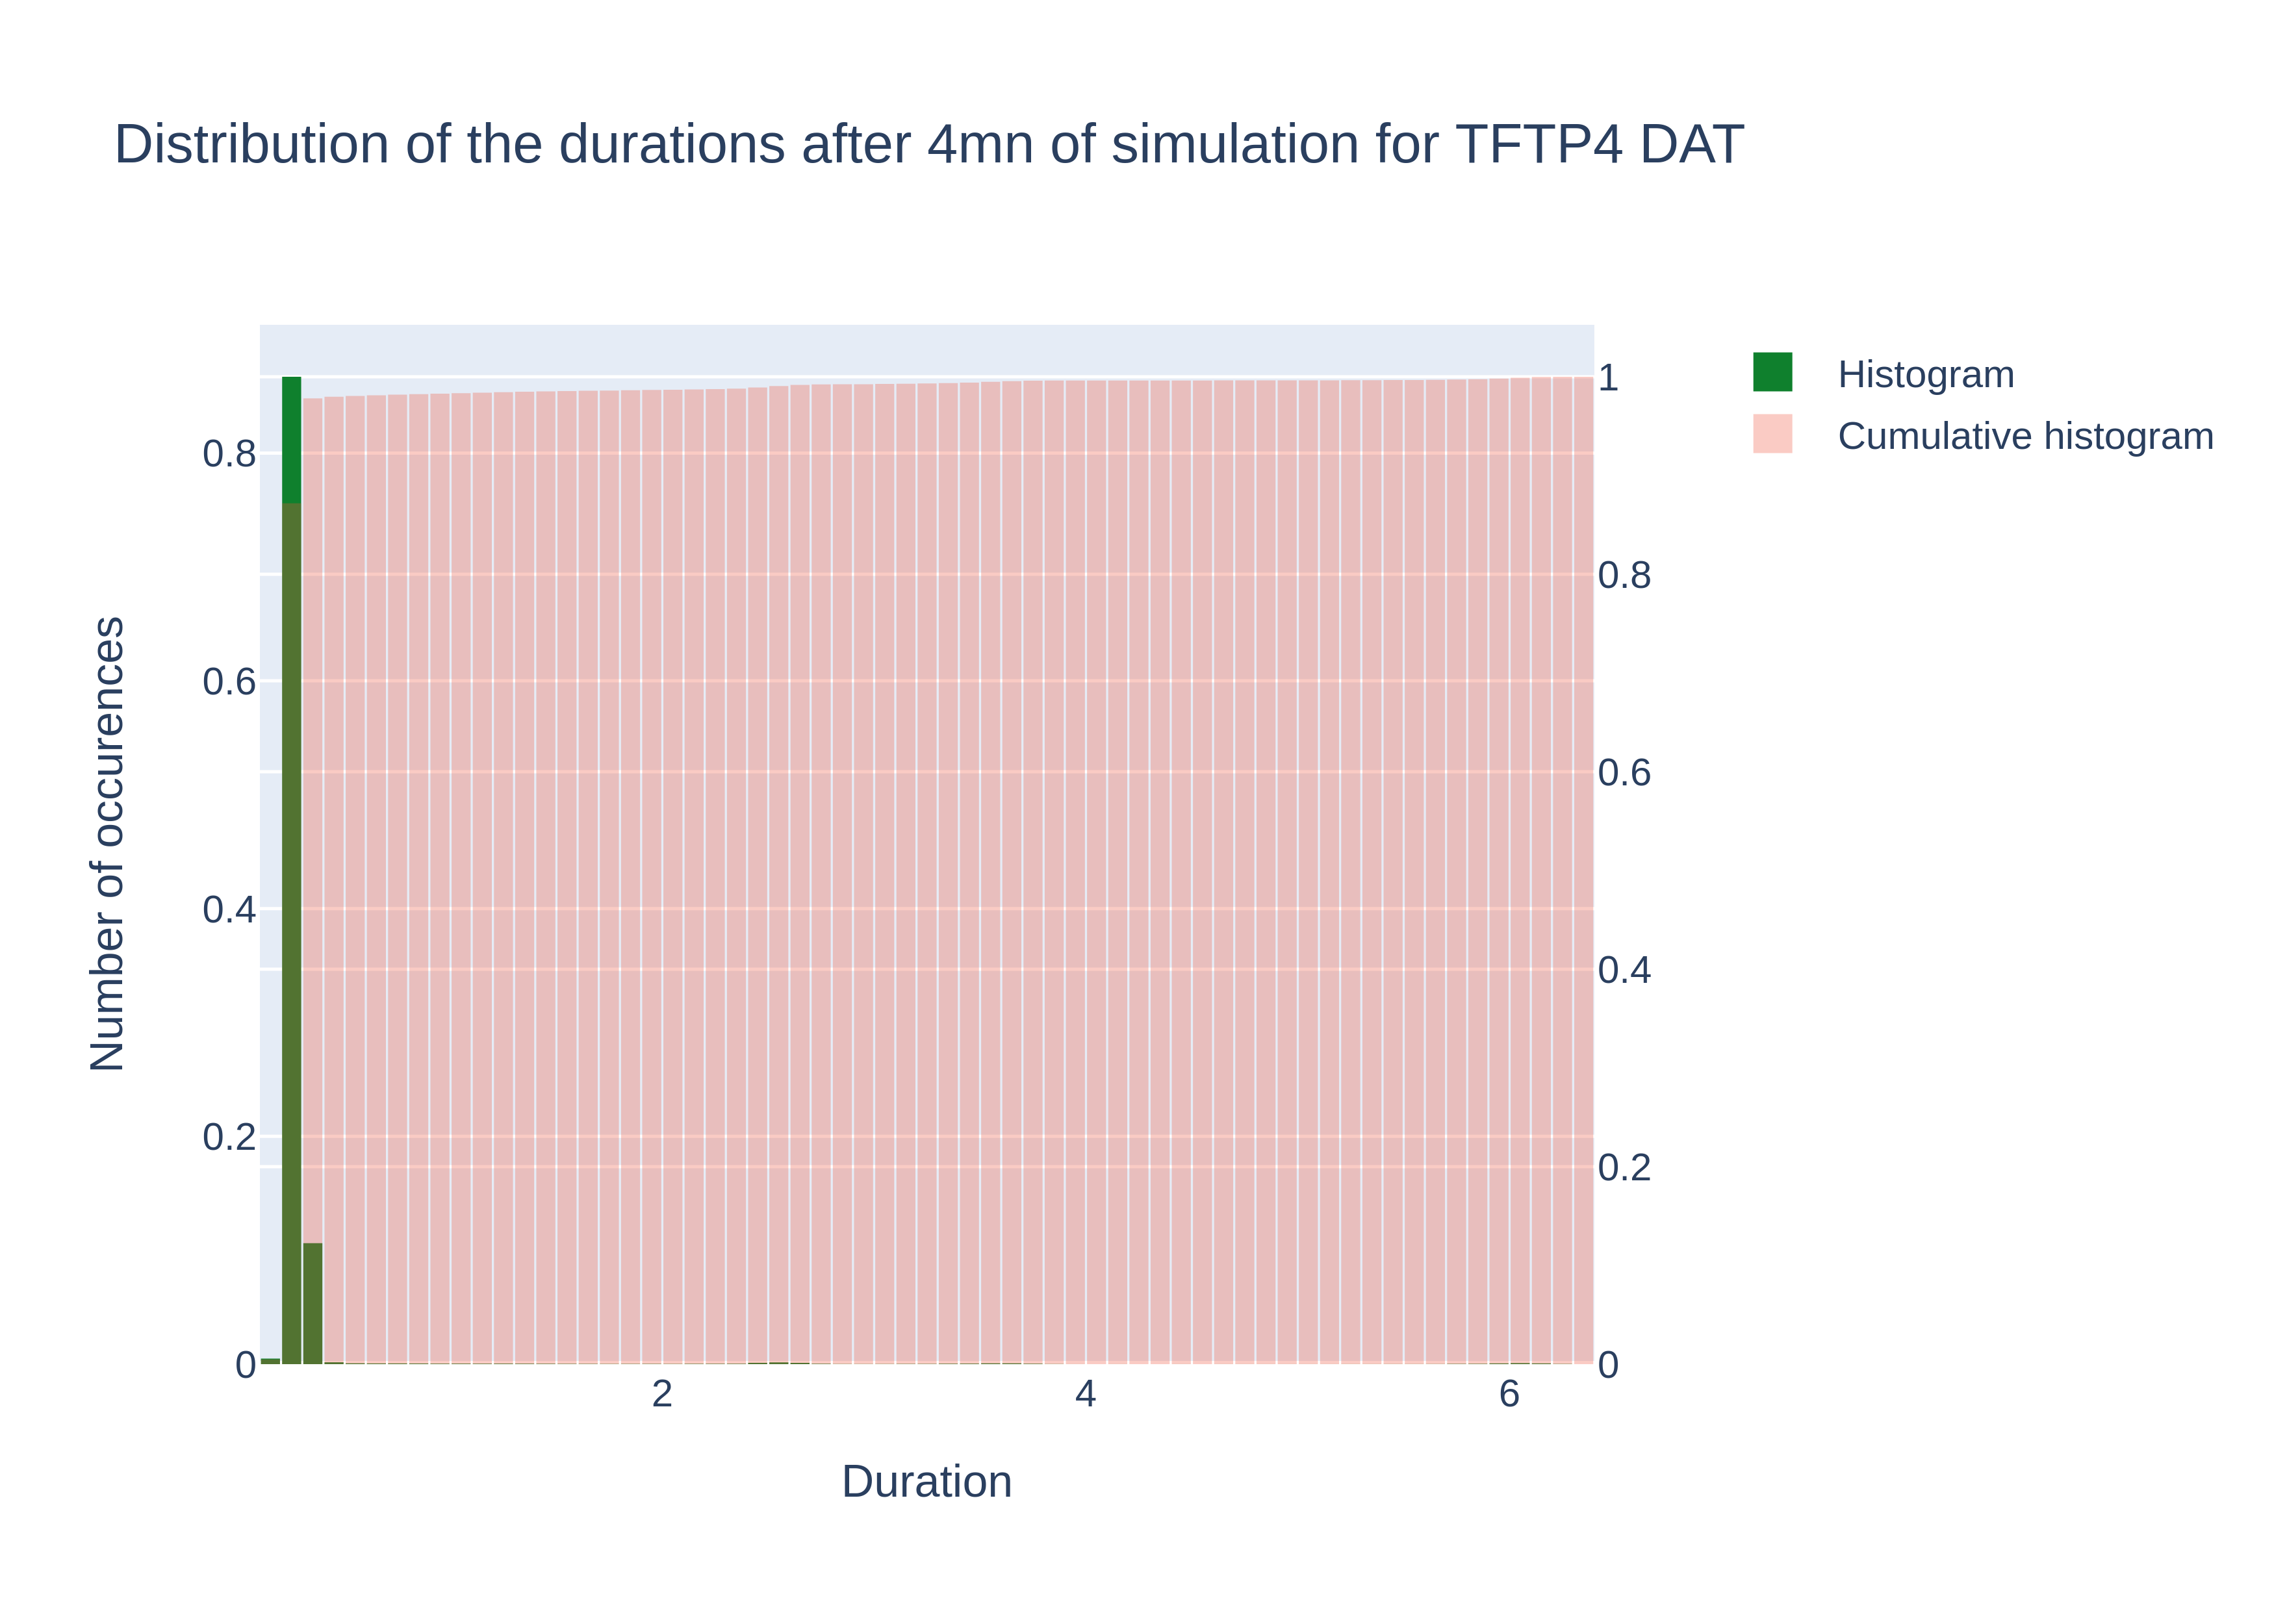
\includegraphics[width=\textwidth]{../fig/data/TFTP4 DAT_4mn.png}
        \caption{Simulation time: 4min}
        \vspace{.5cm}
    \end{subfigure}
    \begin{subfigure}{.495\textwidth}
        \centering
        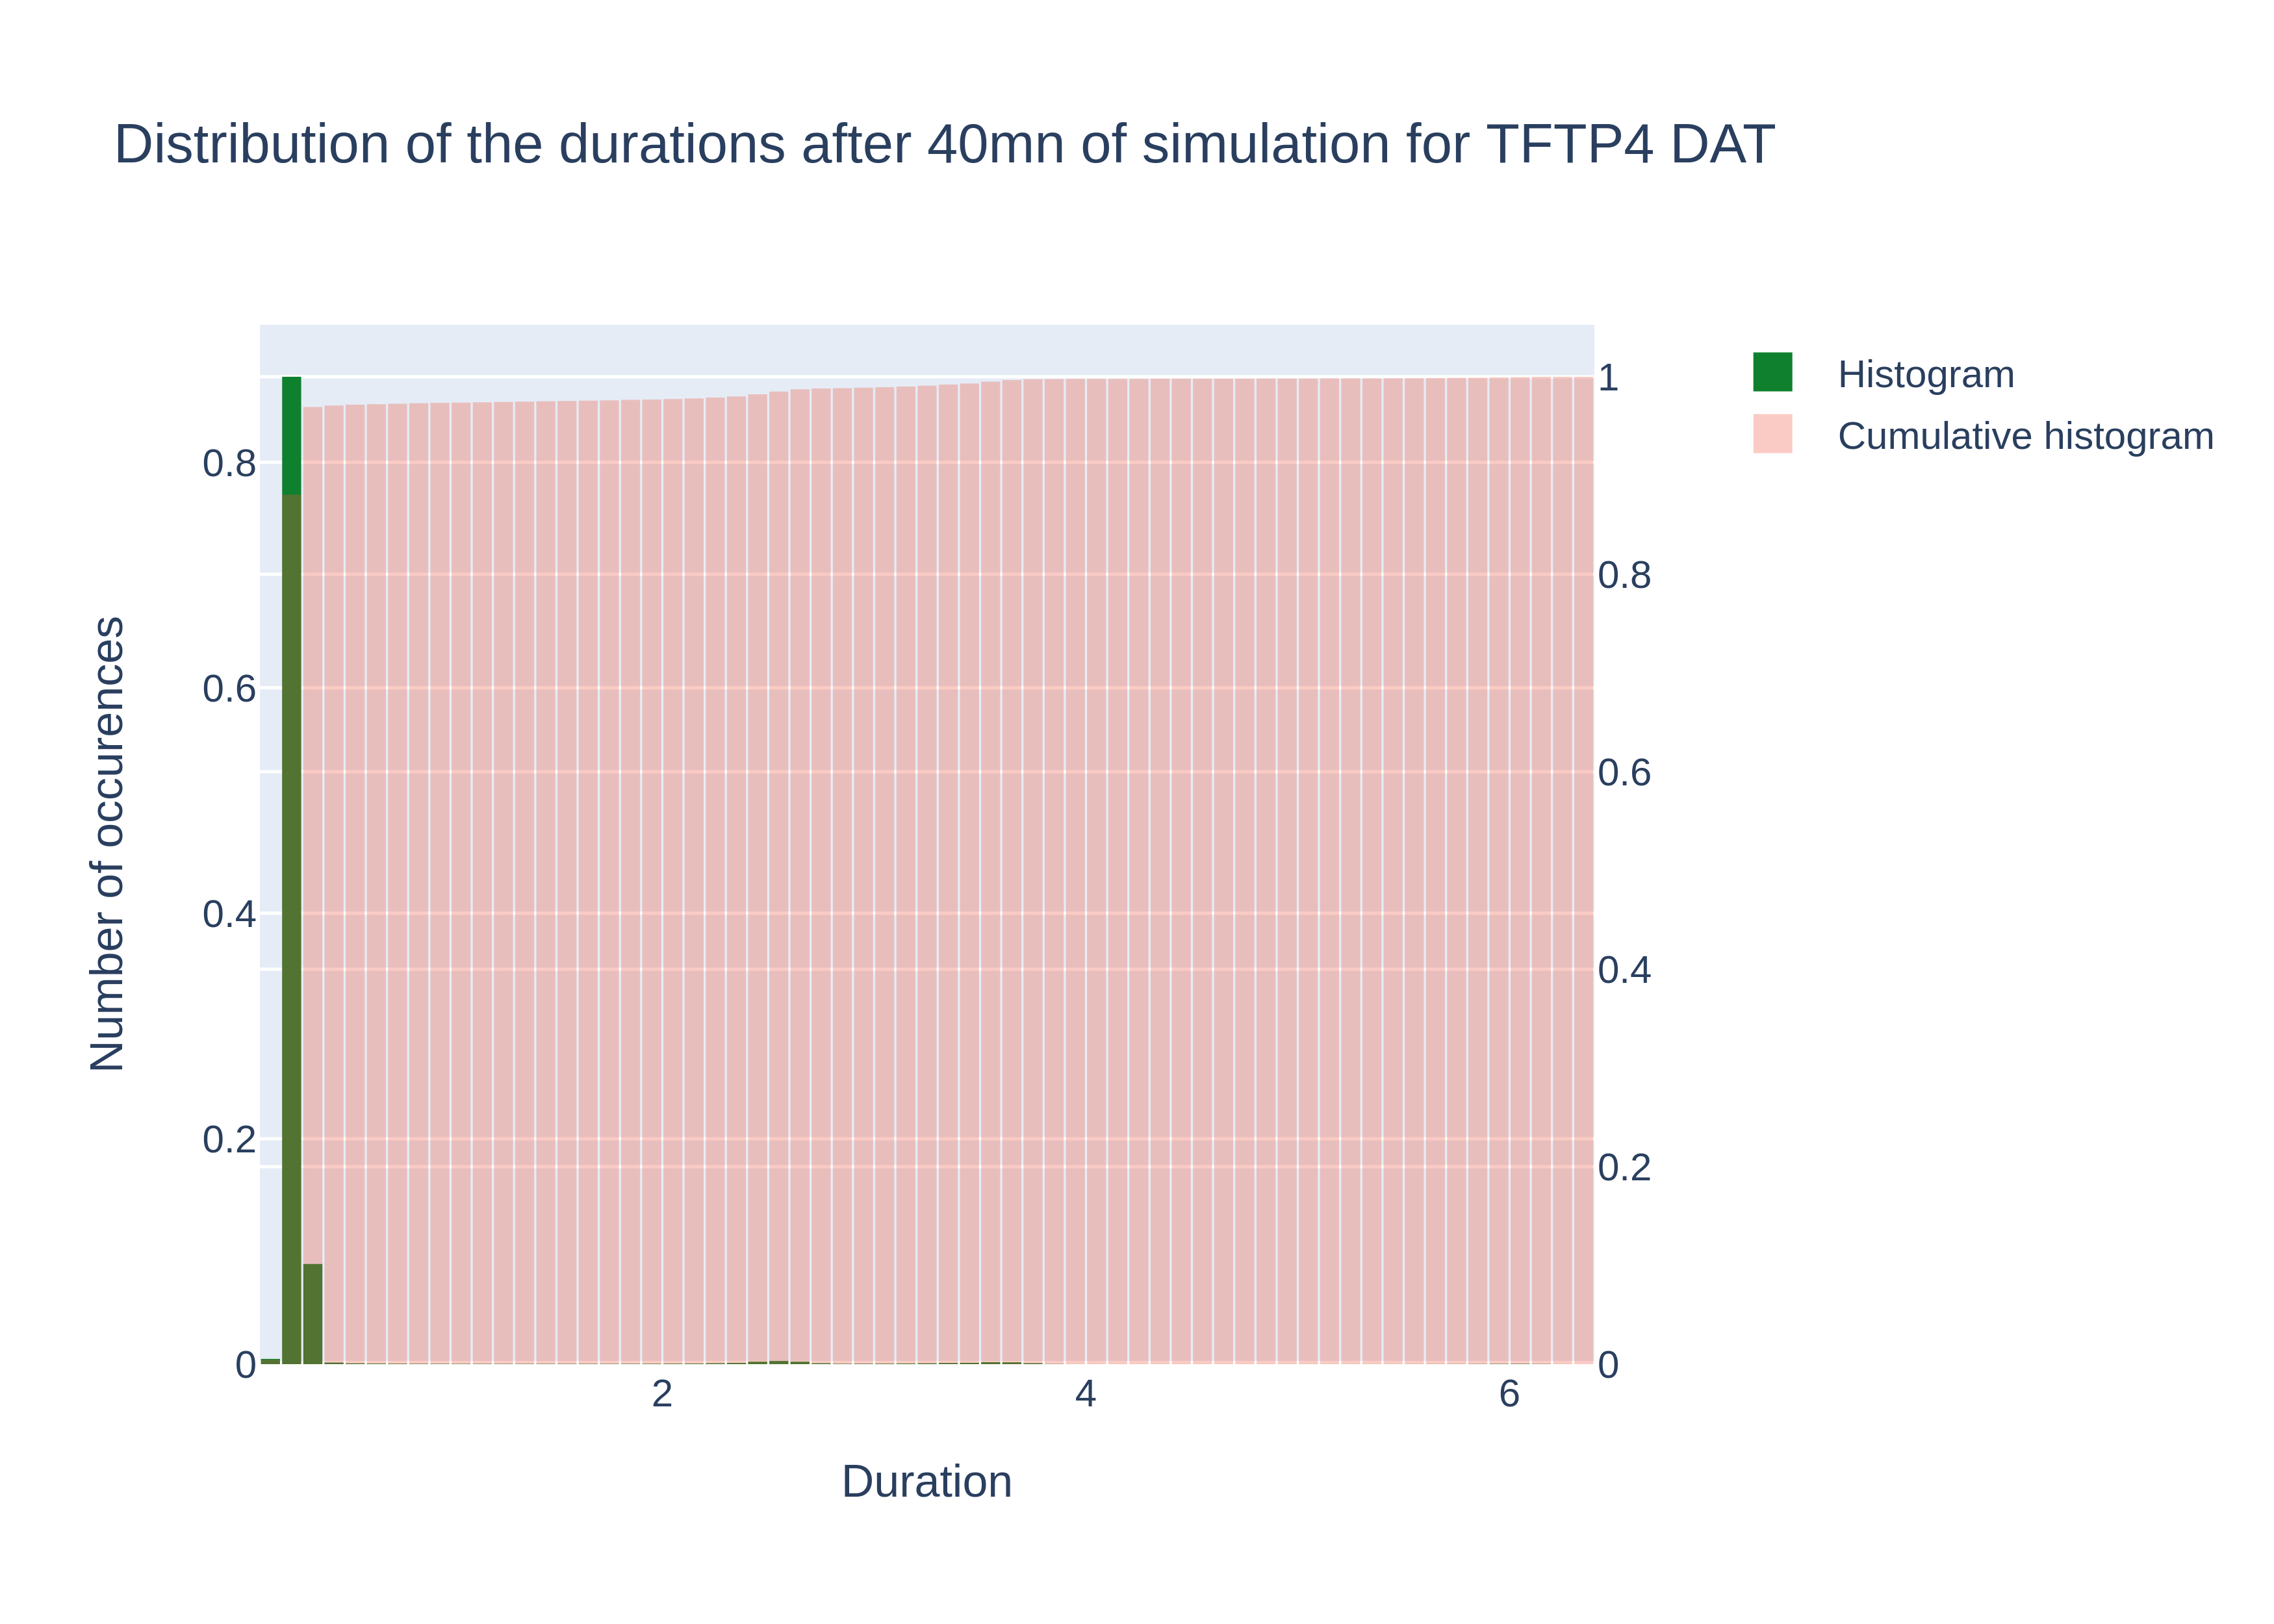
\includegraphics[width=\textwidth]{../fig/data/TFTP4 DAT_40mn.png}
        \caption{Simulation time: 40min}
    \end{subfigure}
    \begin{subfigure}{.495\textwidth}
        \centering
        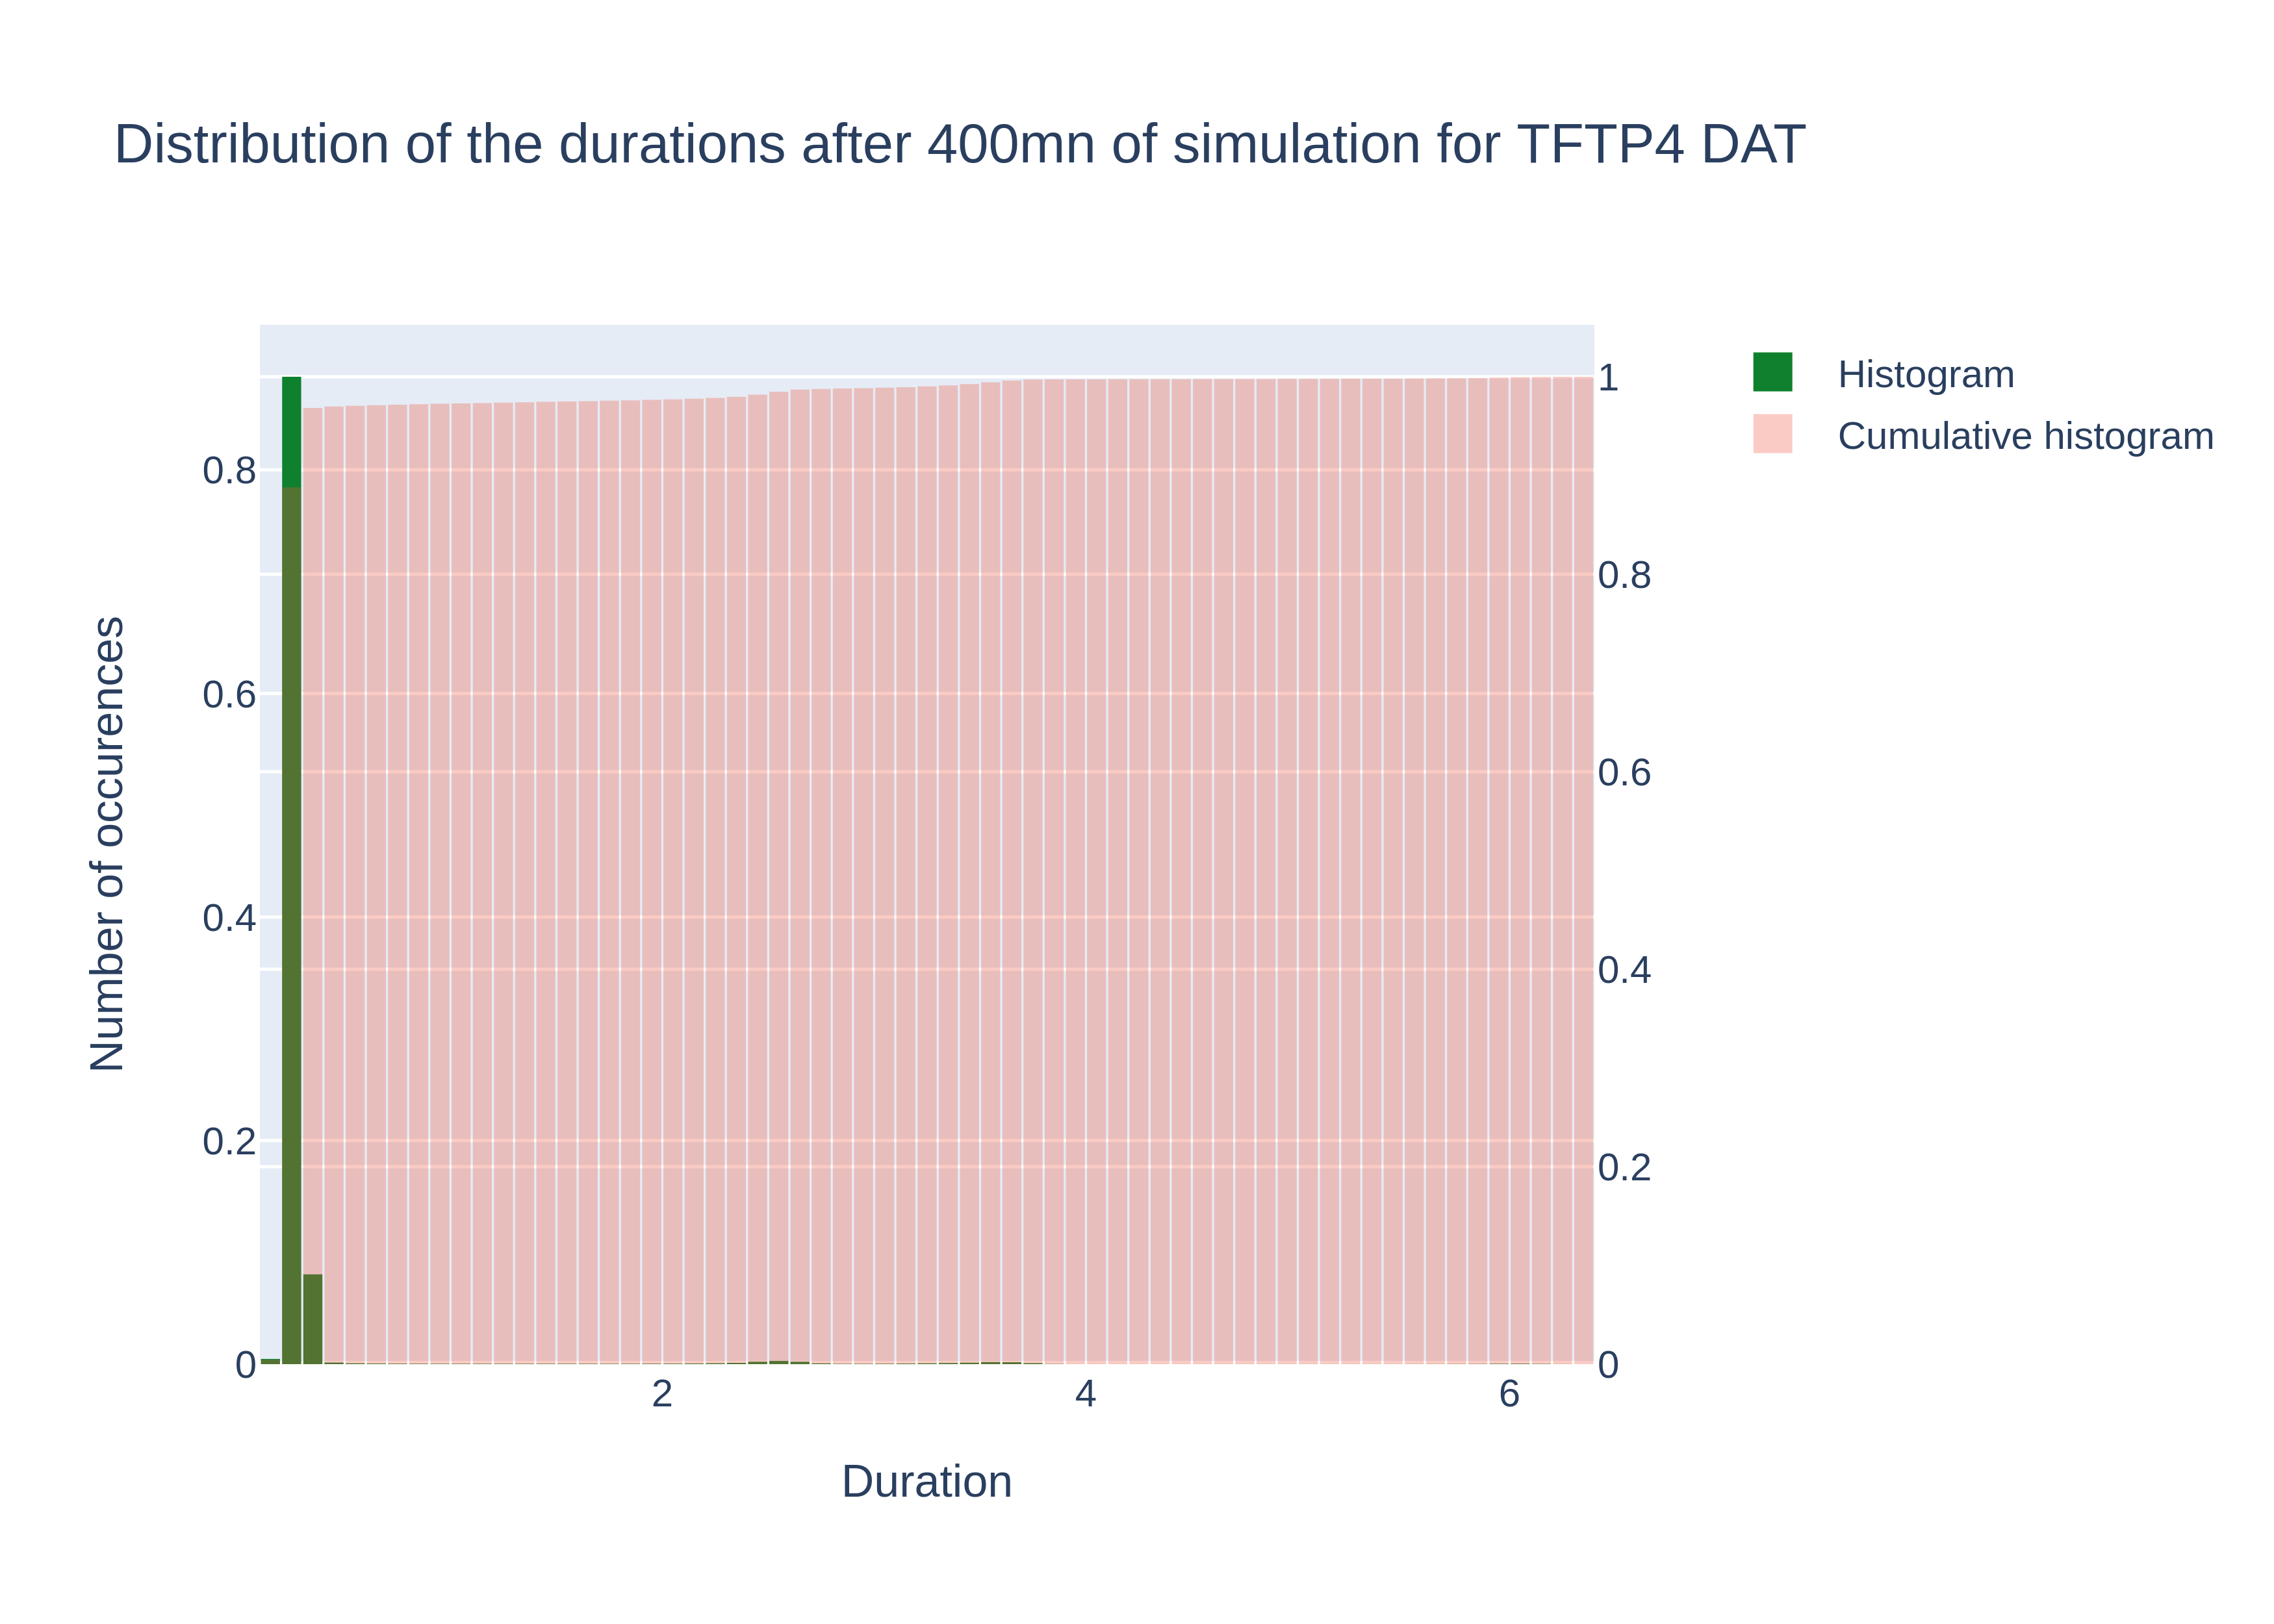
\includegraphics[width=\textwidth]{../fig/data/TFTP4 DAT_400mn.png}
        \caption{Simulation time: 400min}
    \end{subfigure}
    \caption{TFTP4 DAT data after multiple simulation times}
\end{figure}

\subsubsection{Quantile 3}
\begin{figure}[H]
    \centering
    \begin{subfigure}{.495\textwidth}
        \centering
        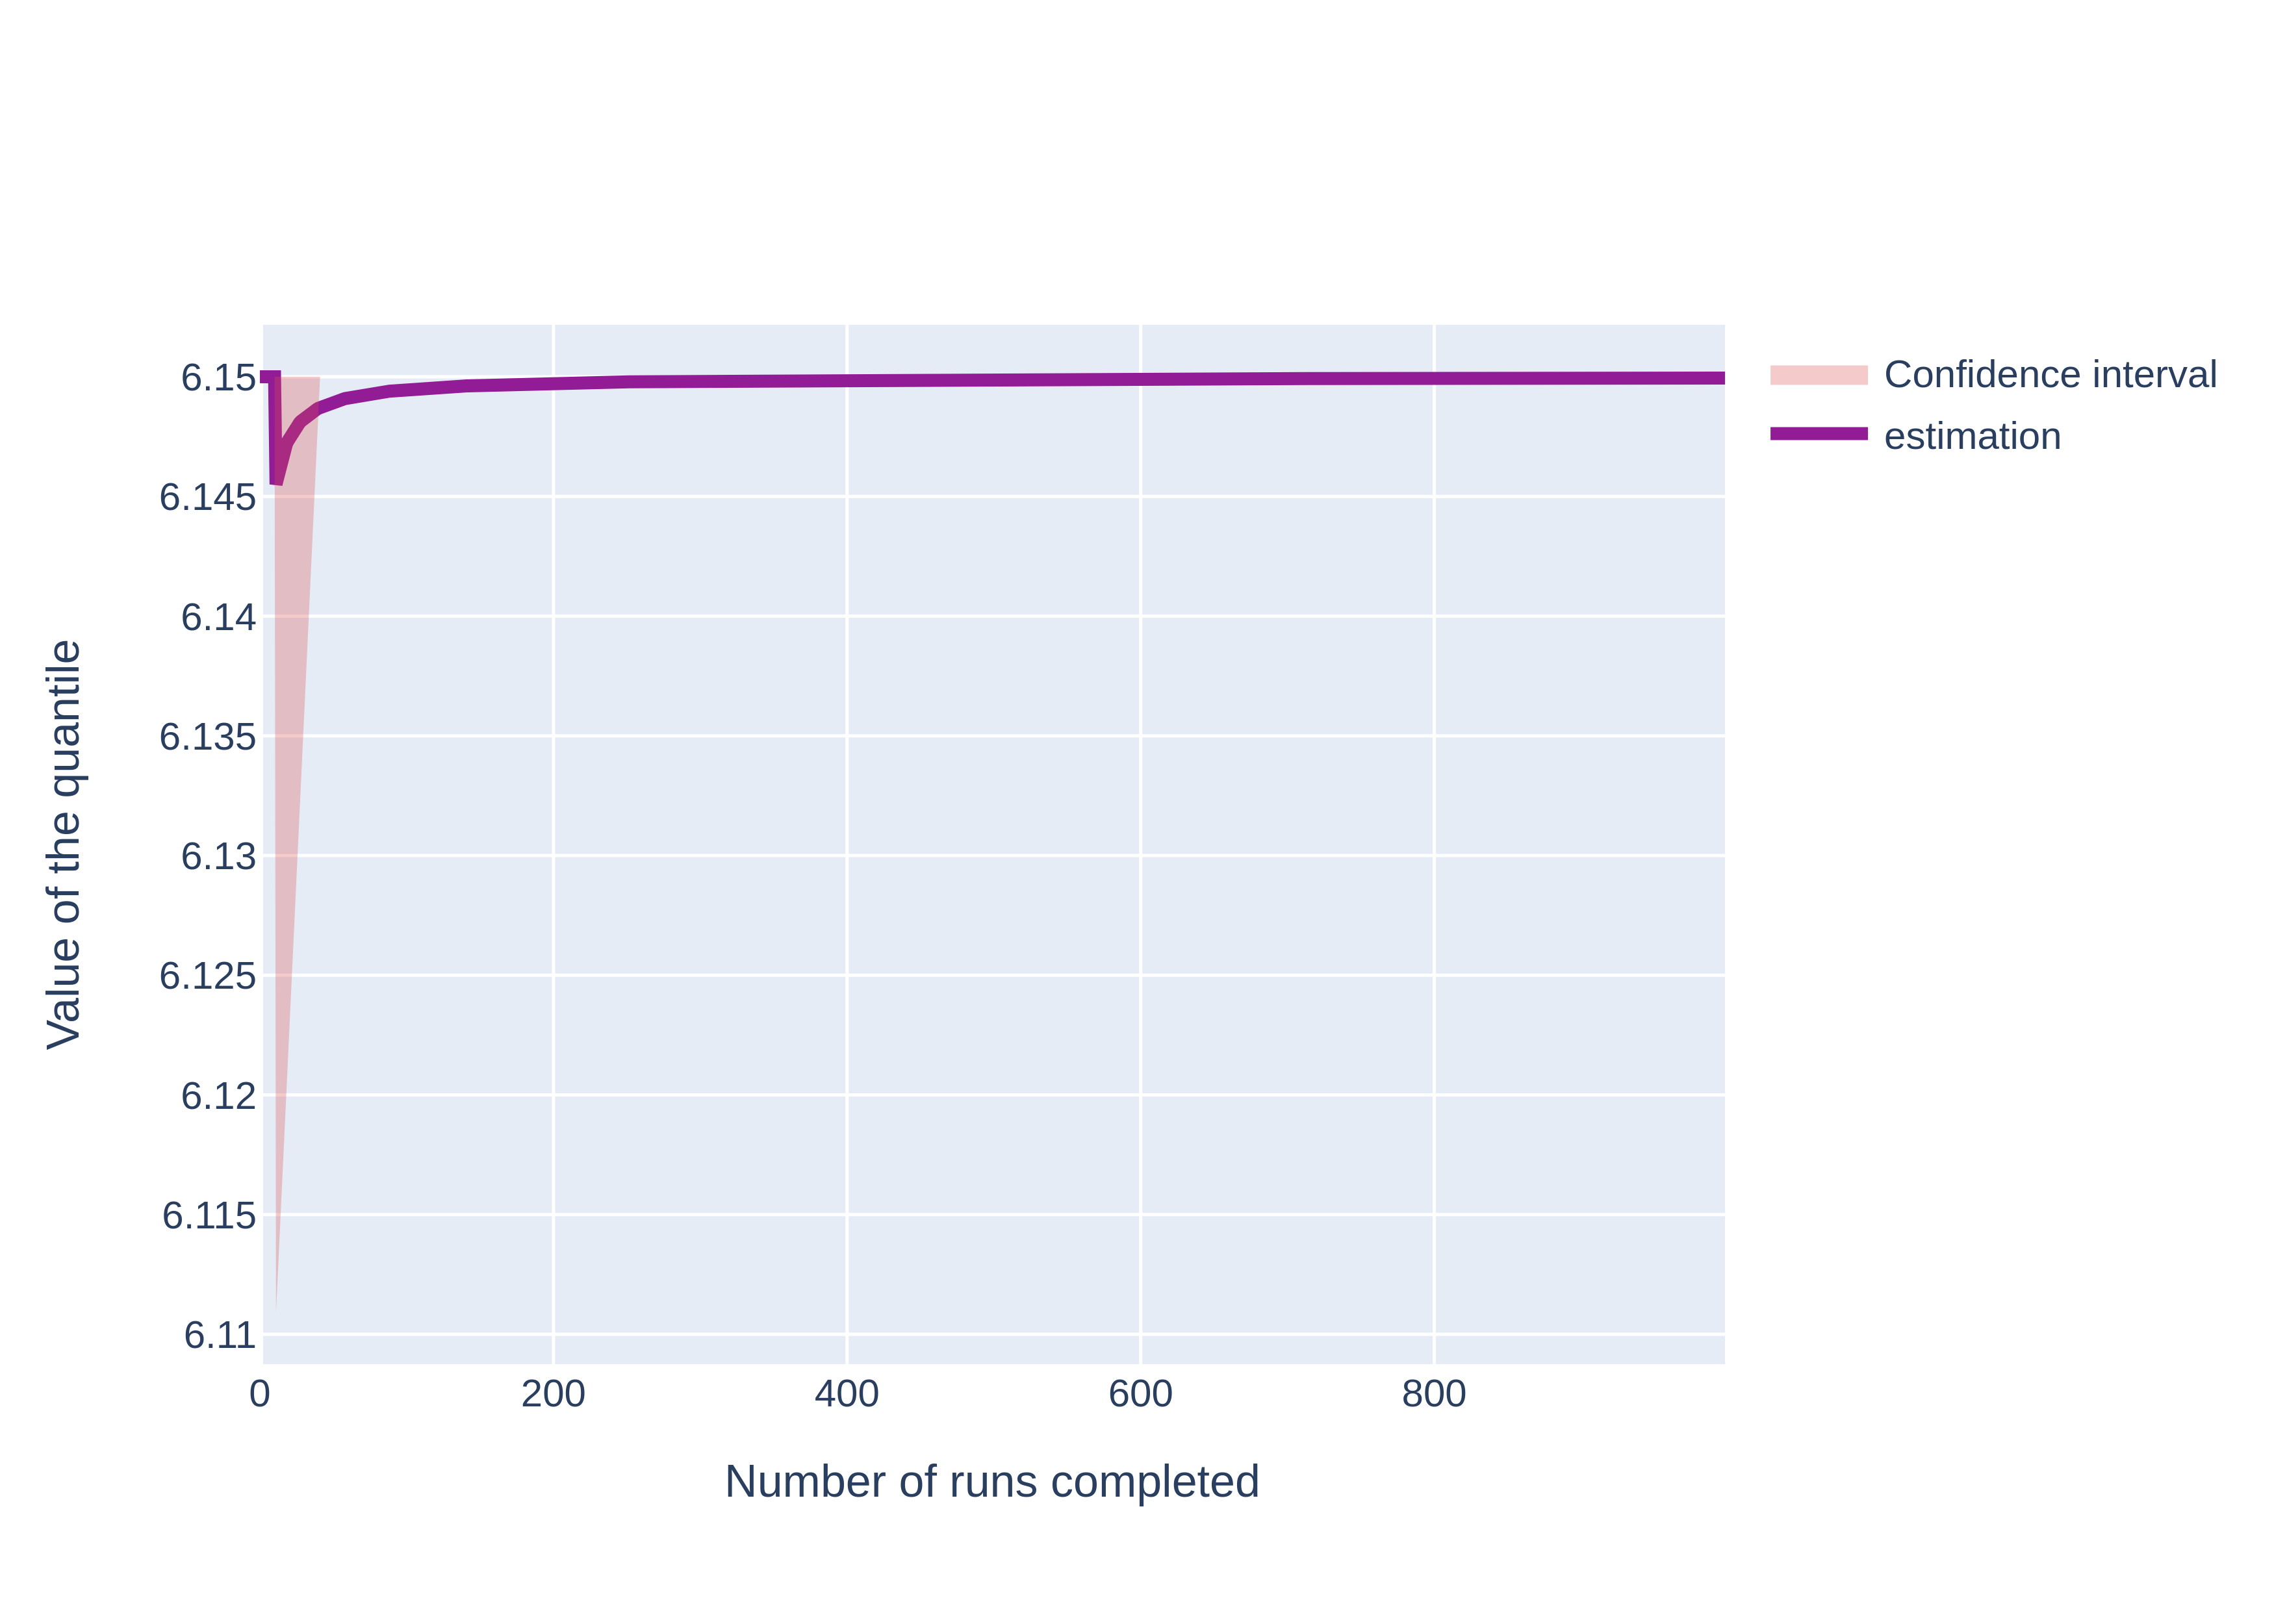
\includegraphics[width=\textwidth]{../fig/quantile3/TFTP4_DAT_24s.png}
        \caption{Simulation time: 24s}
        \vspace{.5cm}
    \end{subfigure}
    \begin{subfigure}{.495\textwidth}
        \centering
        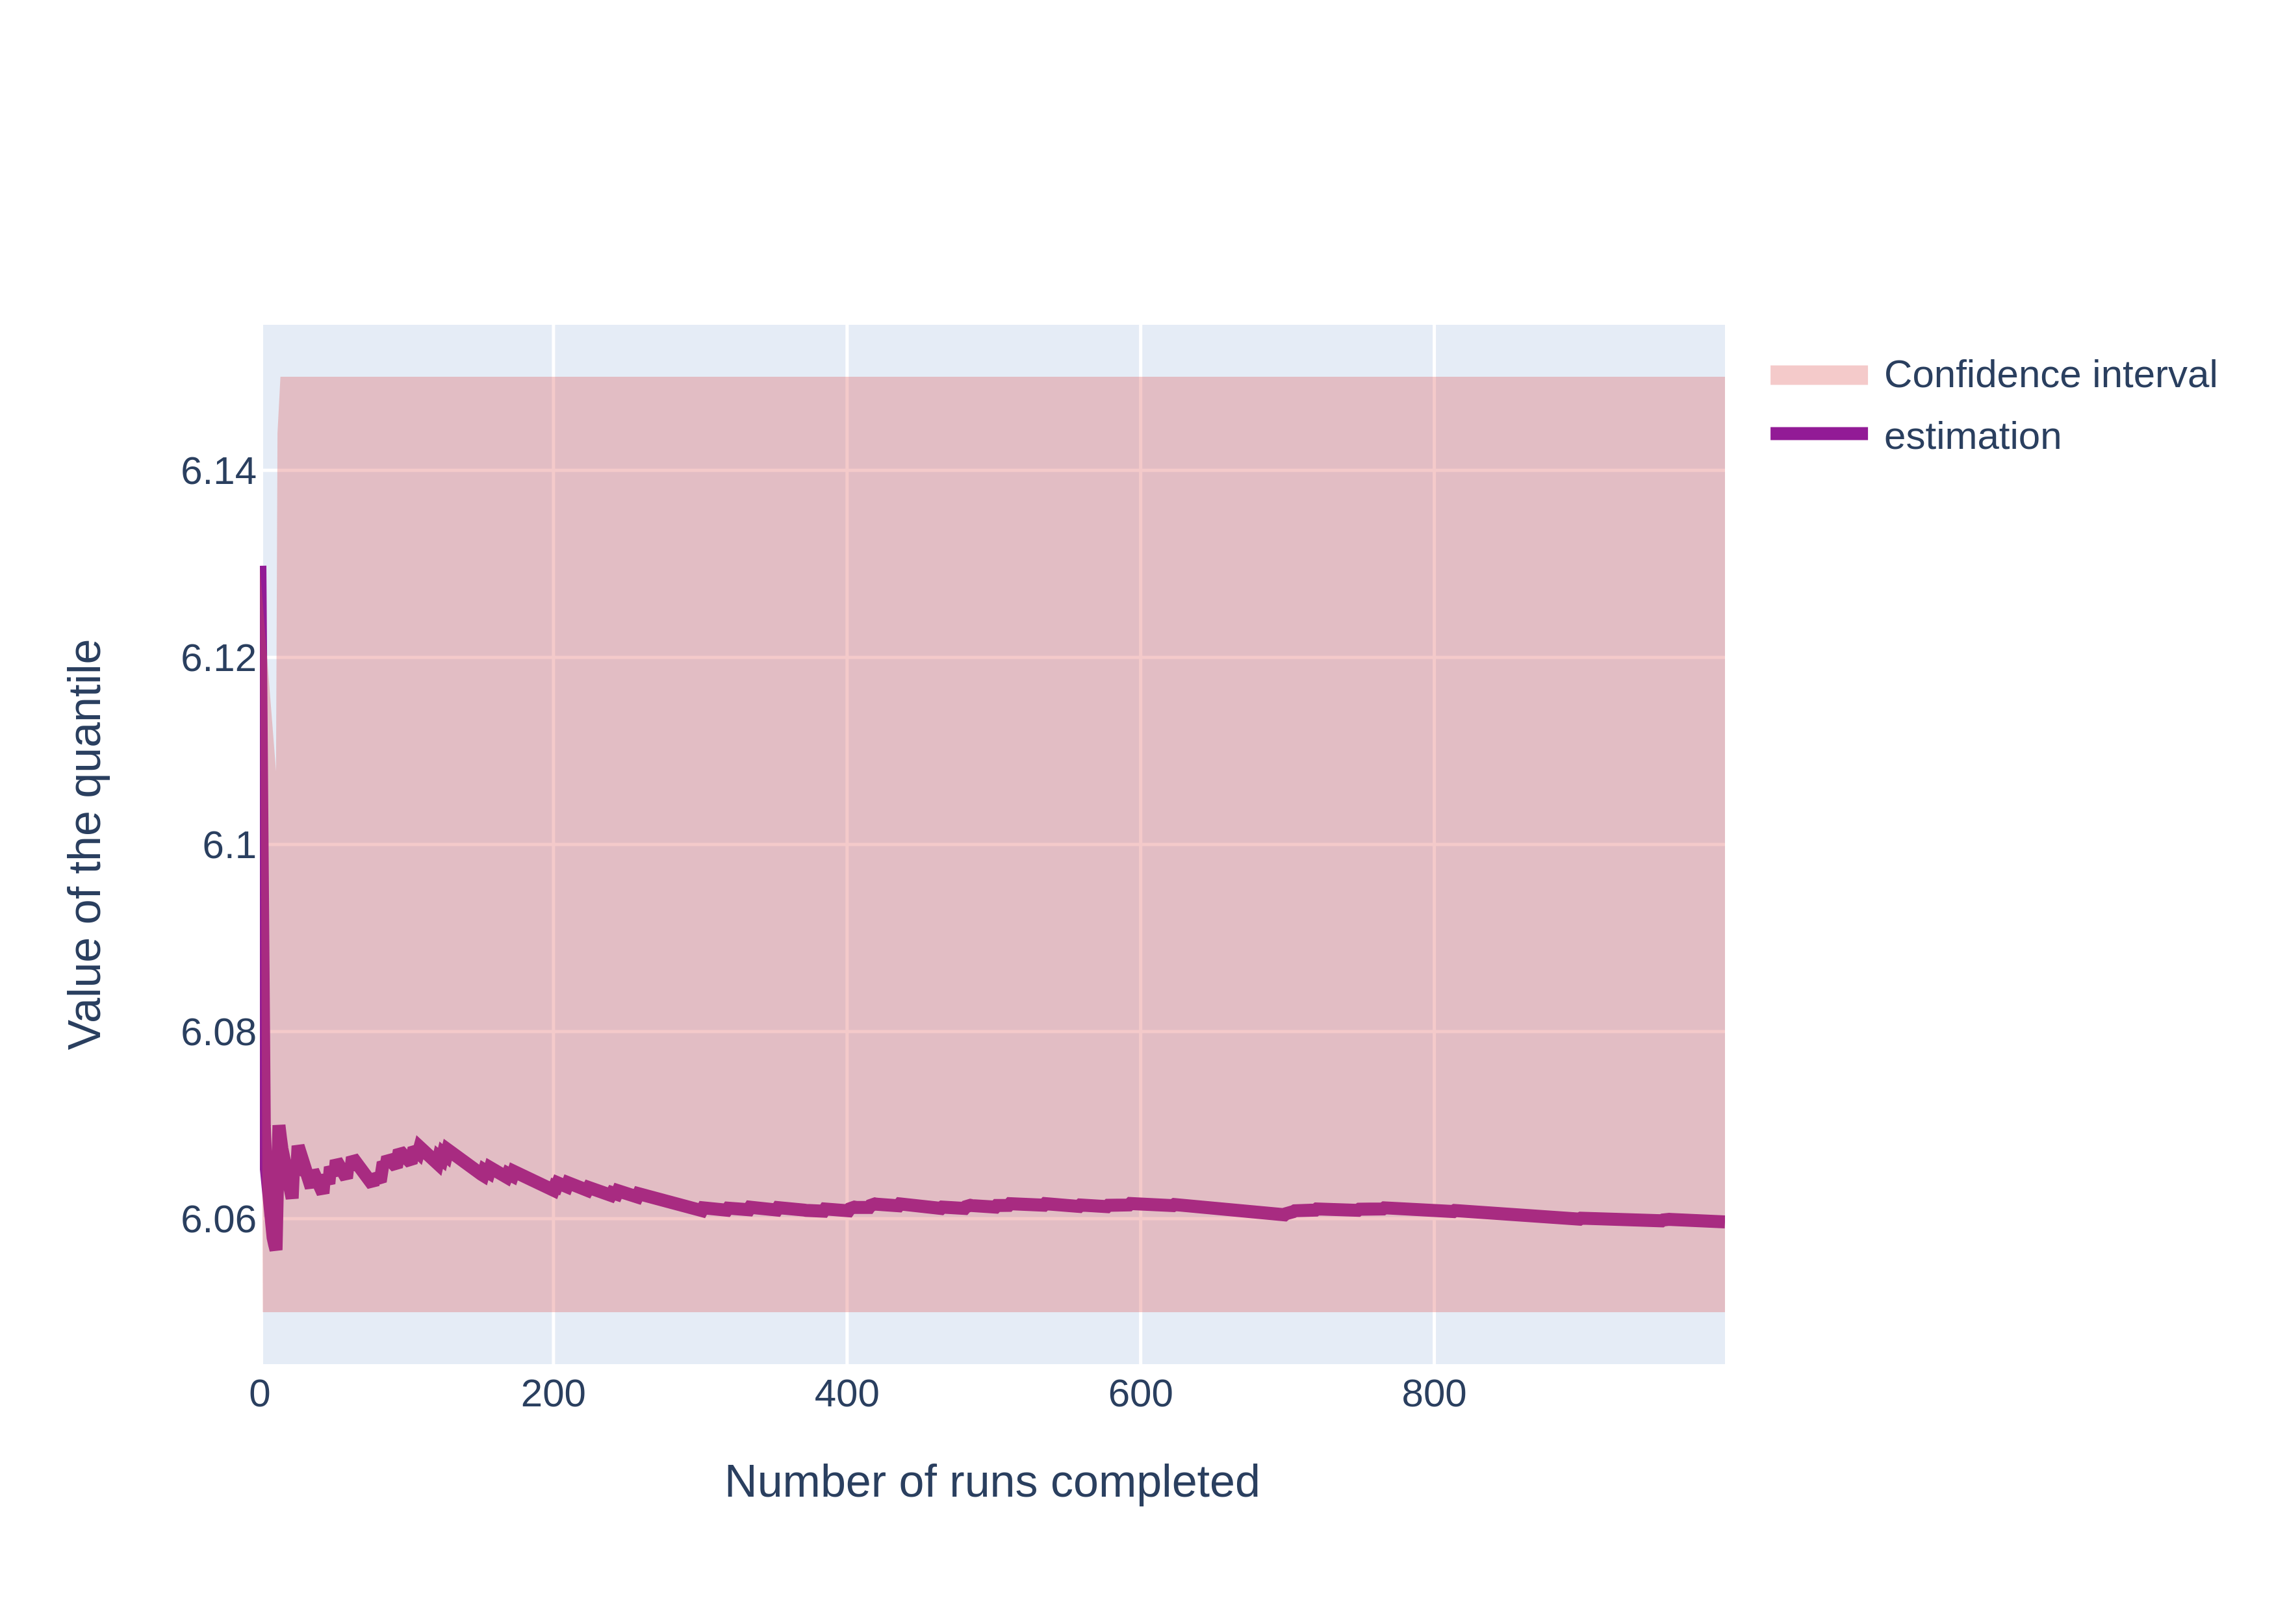
\includegraphics[width=\textwidth]{../fig/quantile3/TFTP4 DAT_4mn.png}
        \caption{Simulation time: 4min}
        \vspace{.5cm}
    \end{subfigure}
    \begin{subfigure}{.495\textwidth}
        \centering
        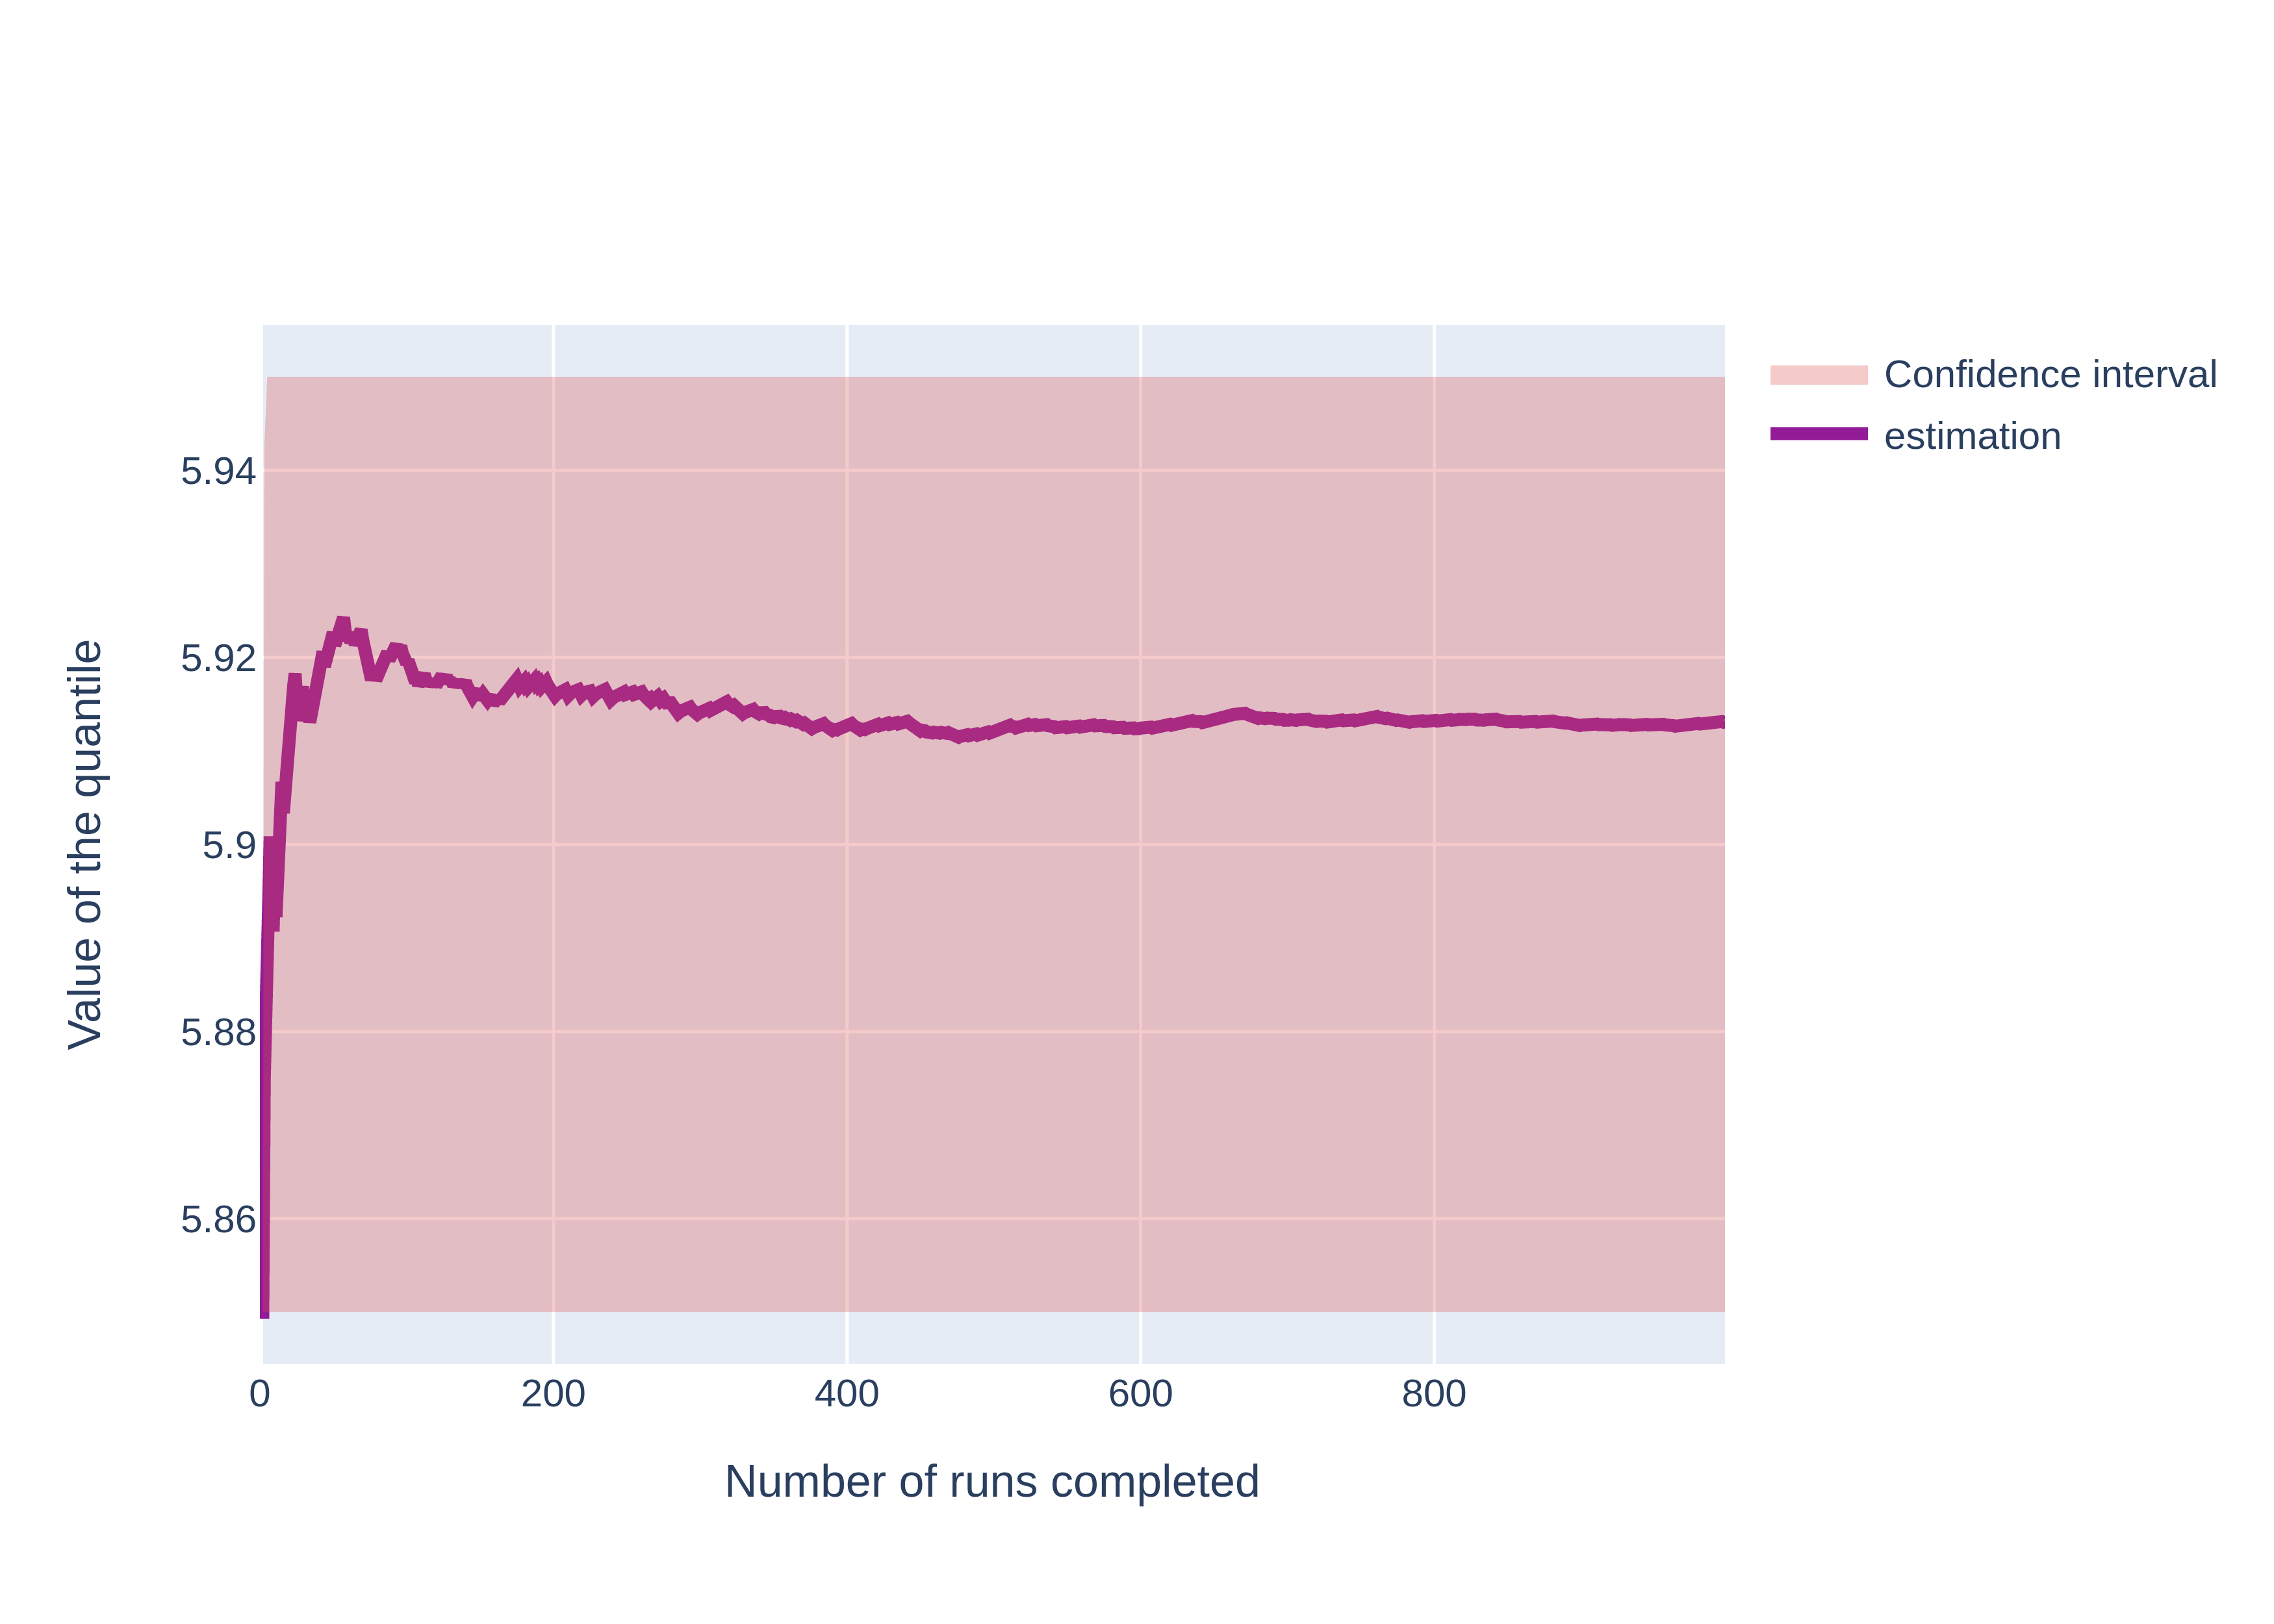
\includegraphics[width=\textwidth]{../fig/quantile3/TFTP4 DAT_40mn.png}
        \caption{Simulation time: 40min}
    \end{subfigure}
    \begin{subfigure}{.495\textwidth}
        \centering
        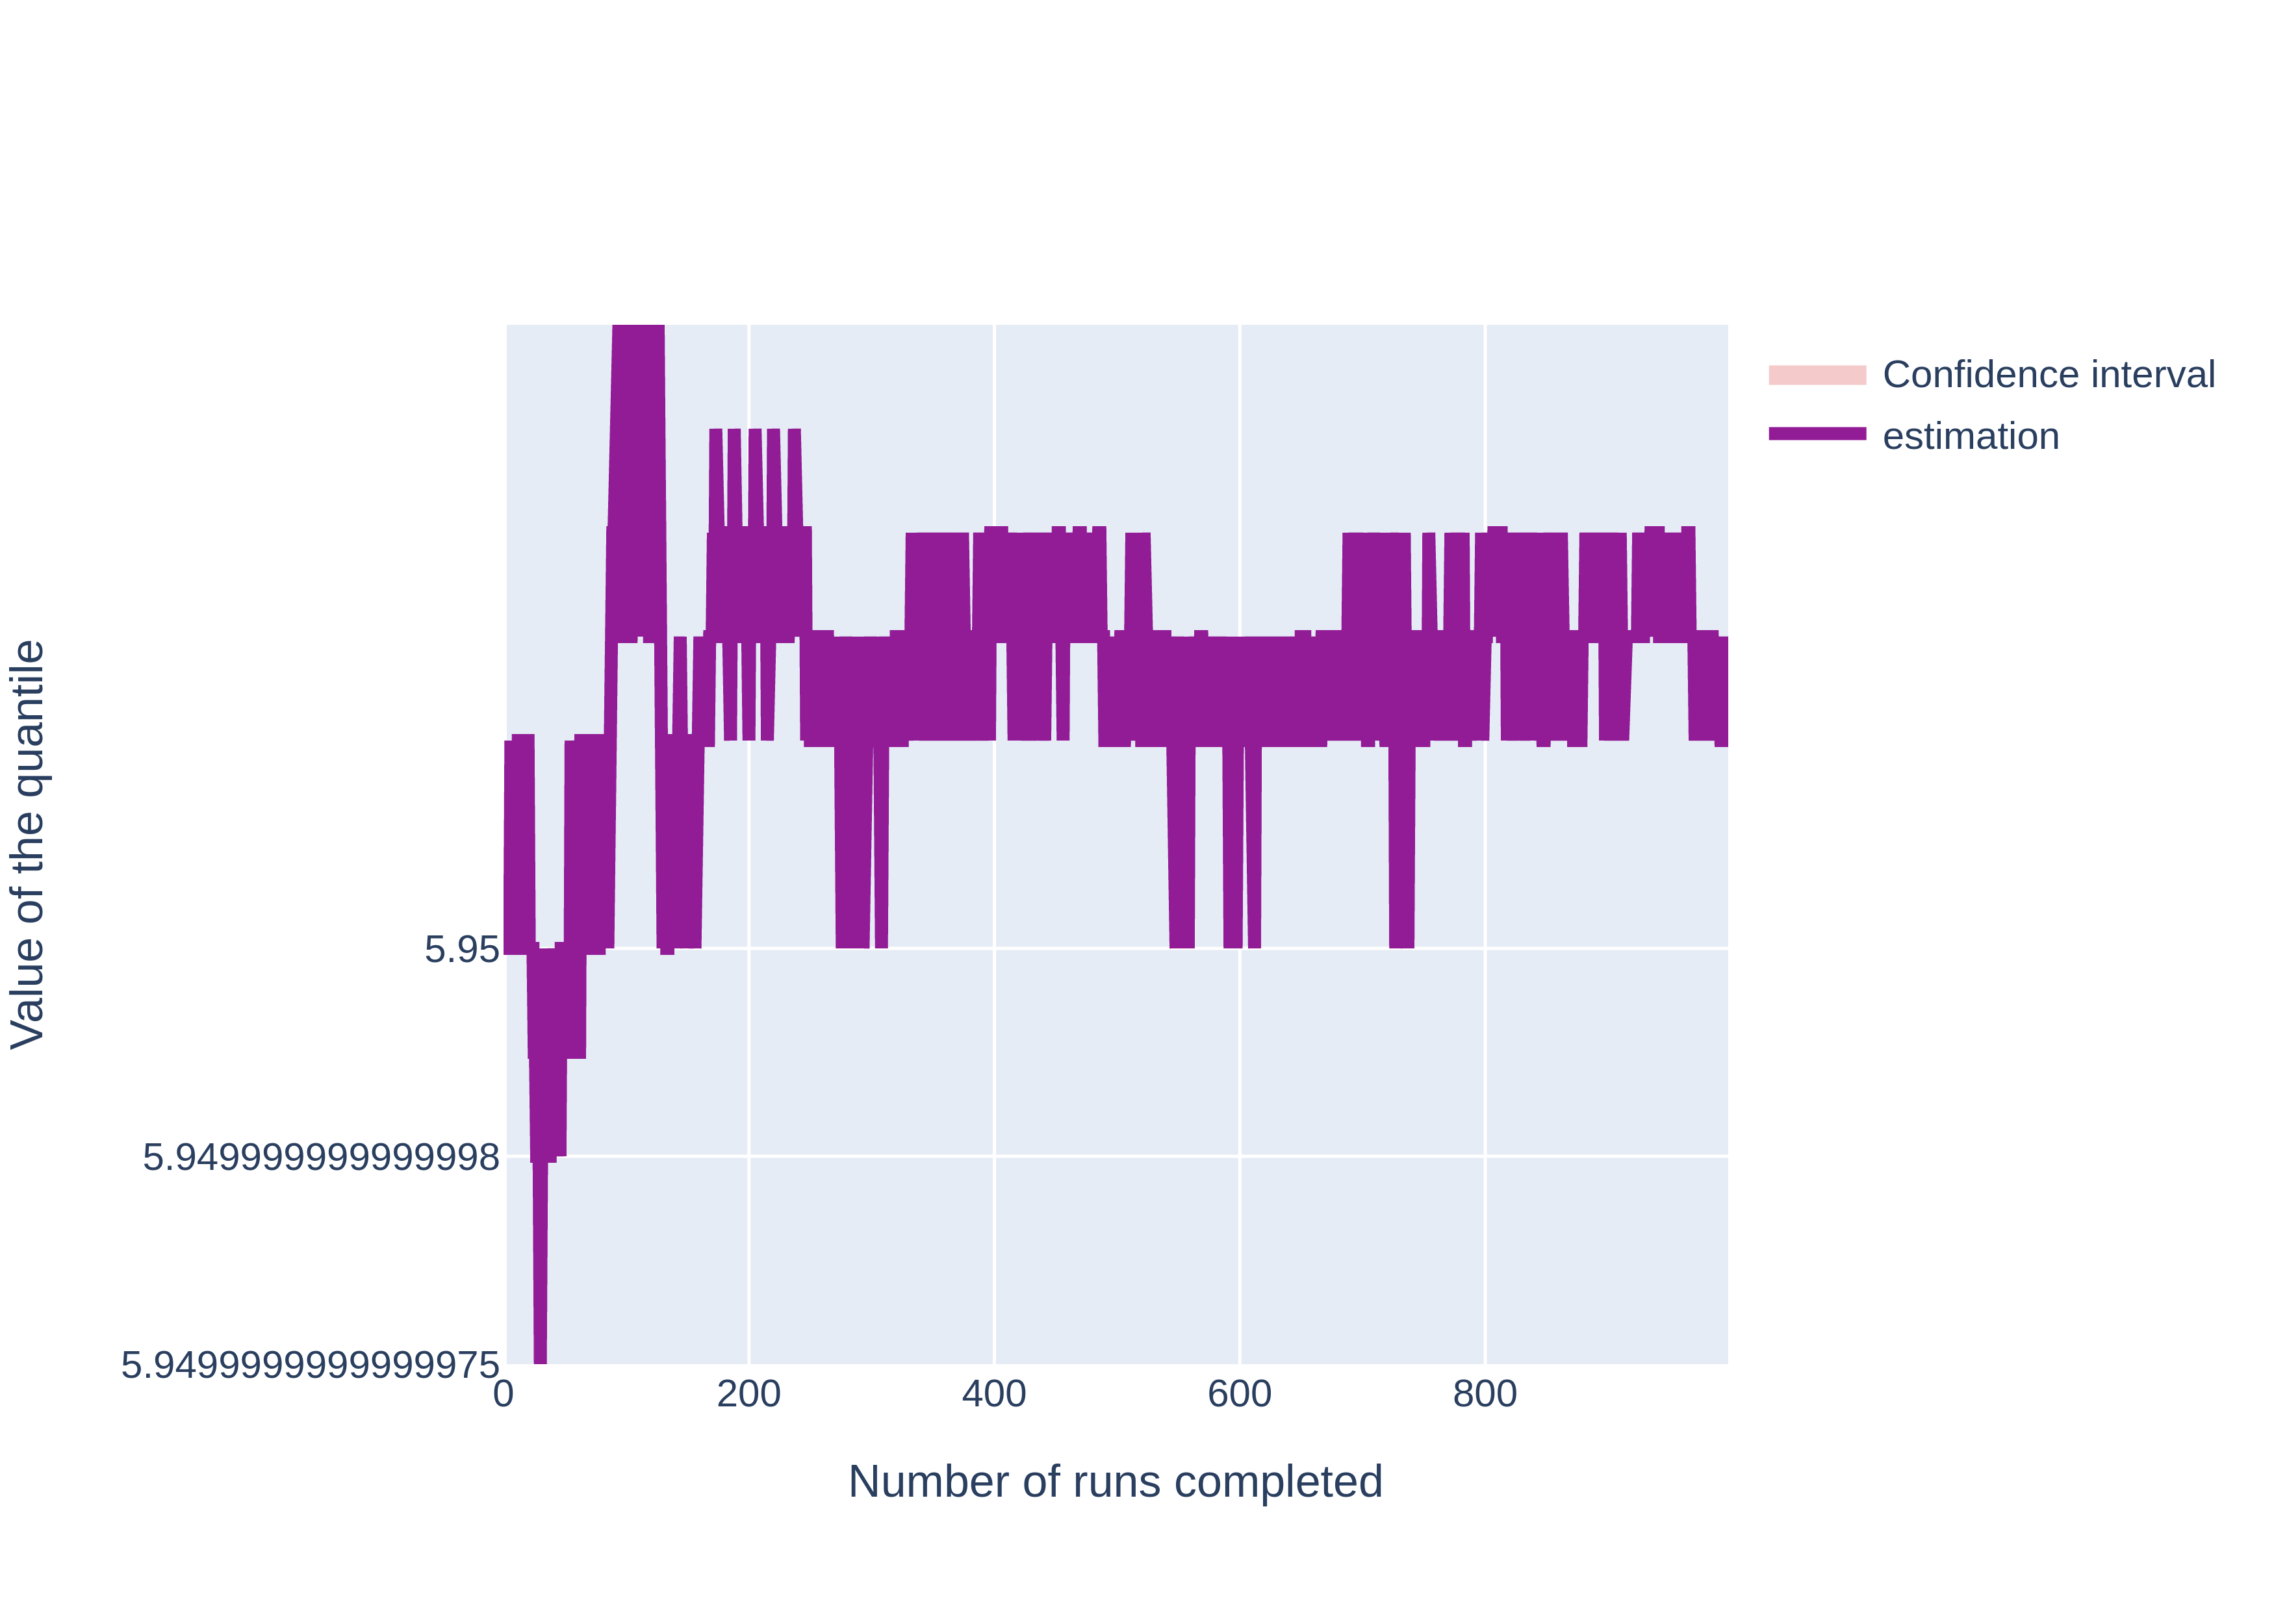
\includegraphics[width=\textwidth]{../fig/quantile3/TFTP4 DAT_400mn.png}
        \caption{Simulation time: 400min}
        \label{fig: TFTP4 DAT q3 400 min}
    \end{subfigure}
    \caption{TFTP4 DAT $q_3$ after multiple simulation times}
\end{figure}

\subsubsection{Quantile 4}
\begin{figure}[H]
    \centering
    \begin{subfigure}{.495\textwidth}
        \centering
        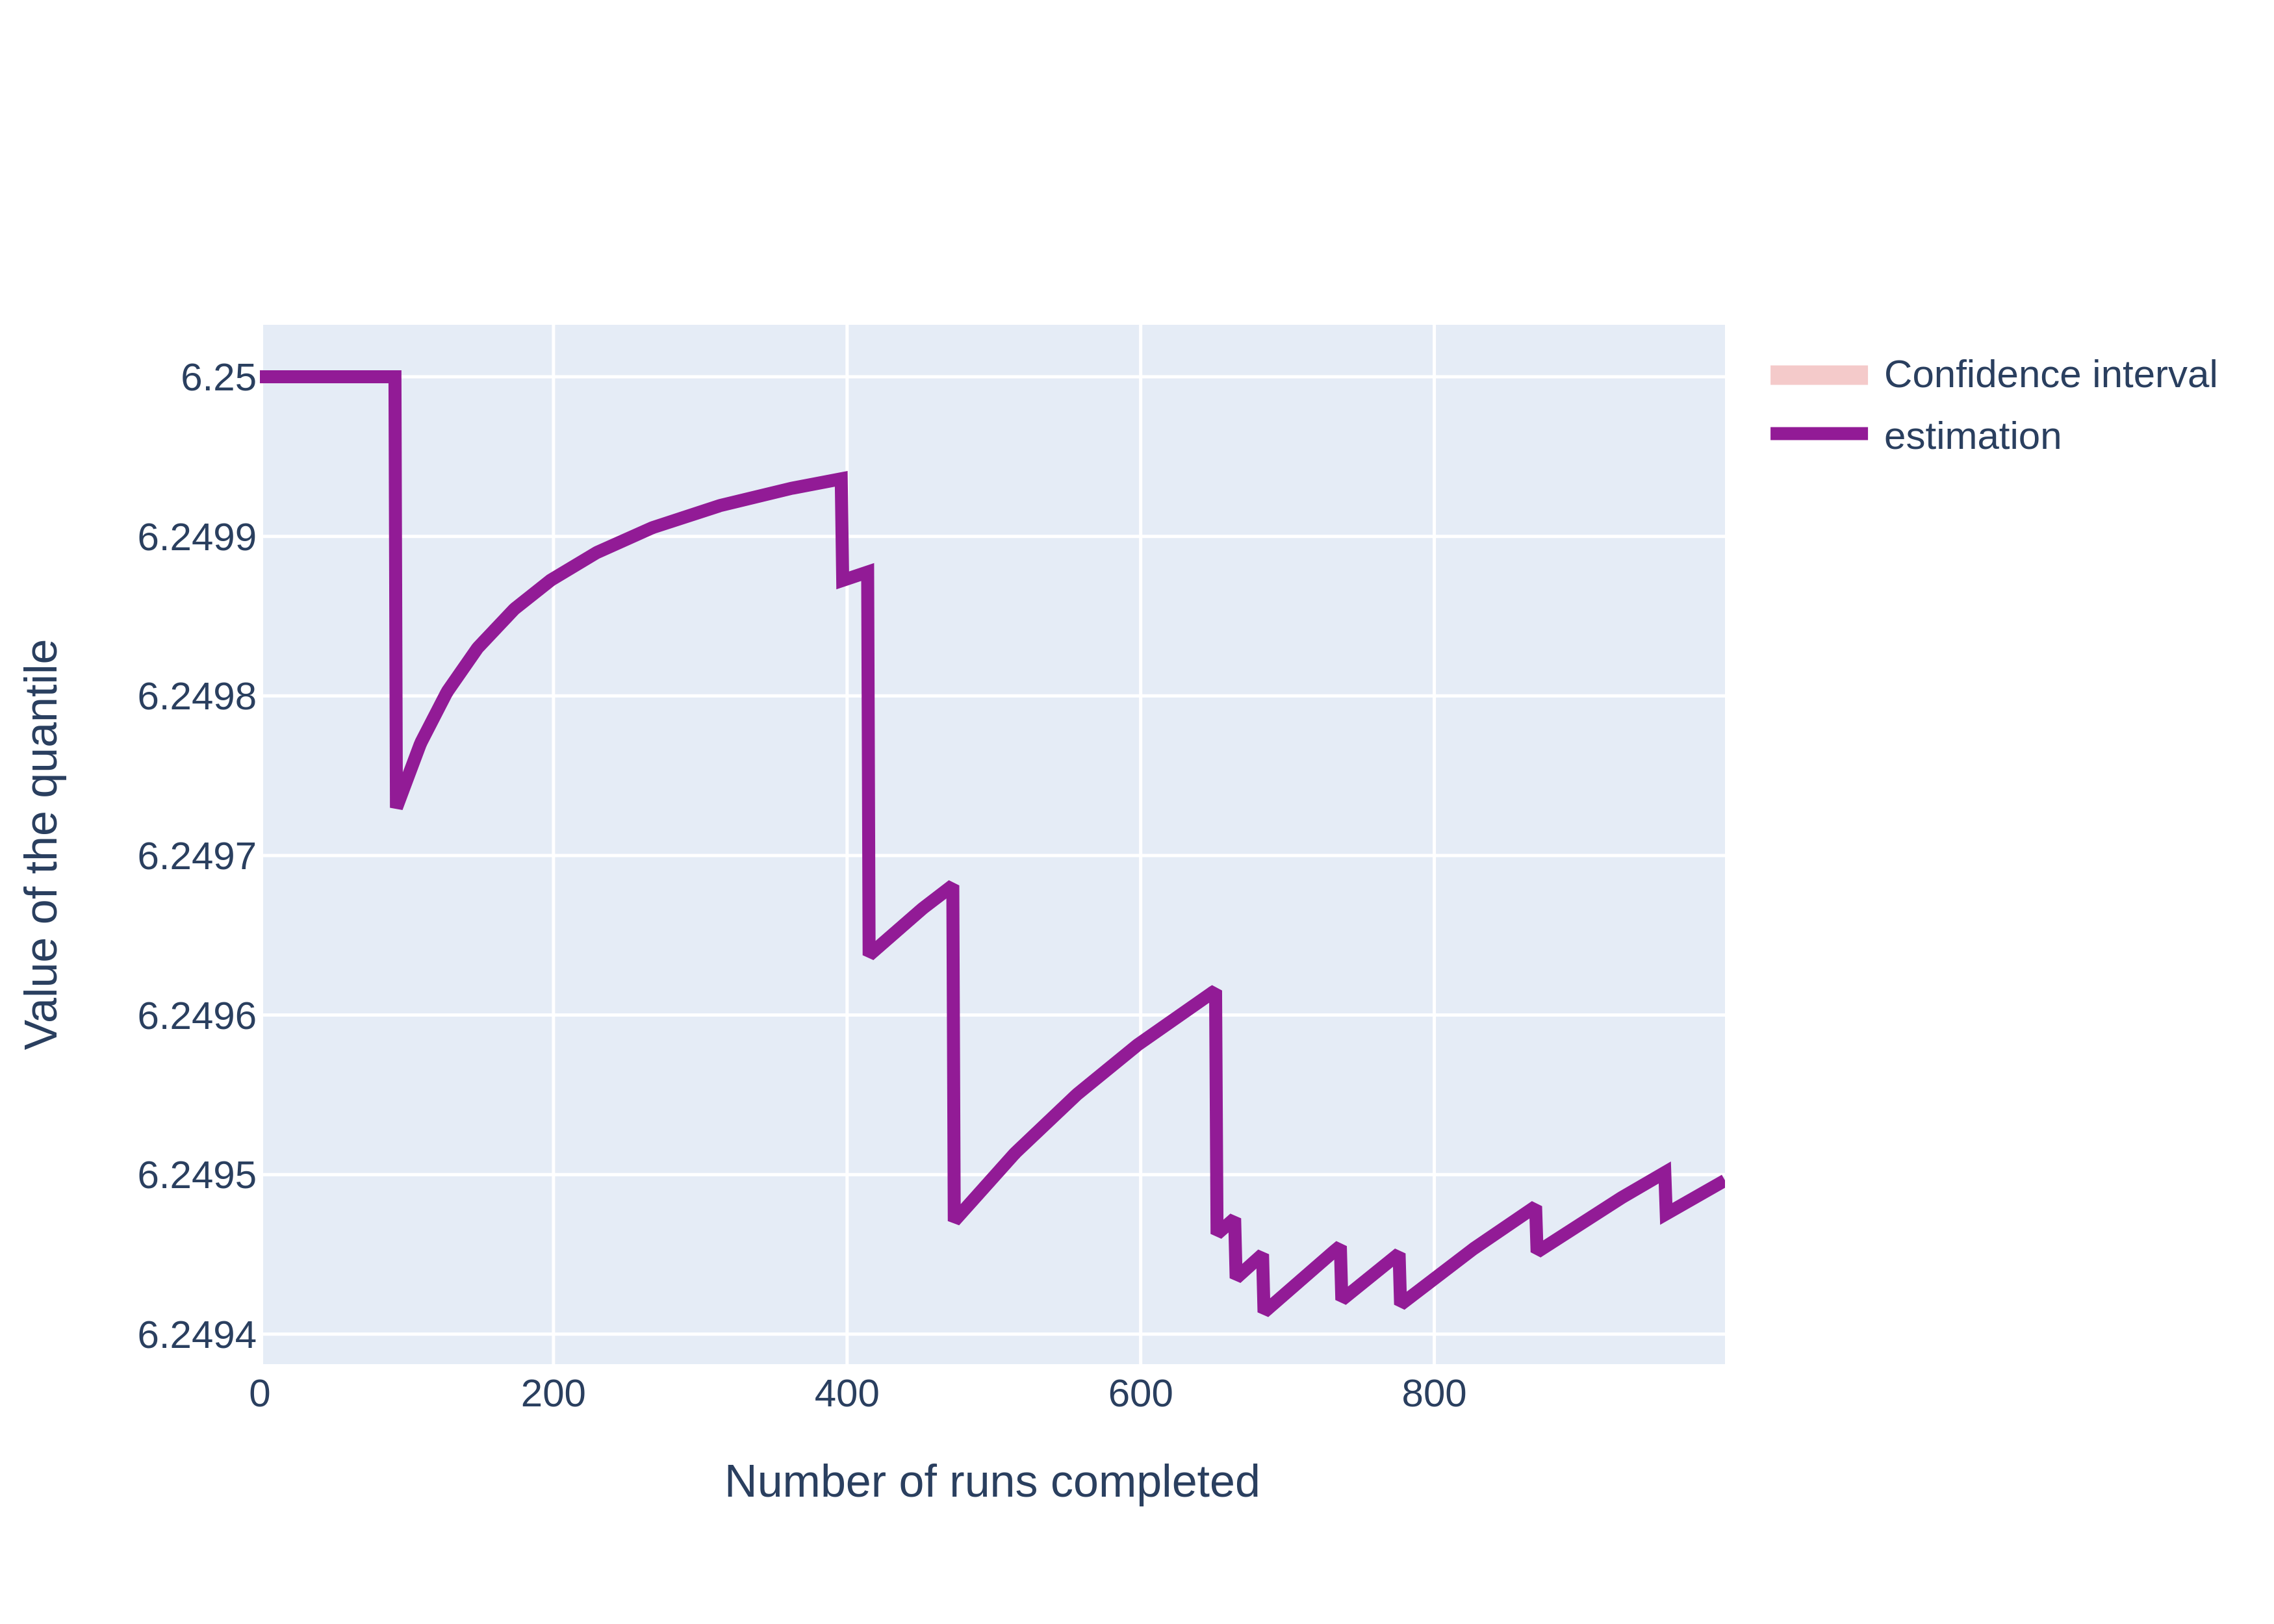
\includegraphics[width=\textwidth]{../fig/quantile4/TFTP4_DAT_24s.png}
        \caption{Simulation time: 24s}
        \vspace{.5cm}
    \end{subfigure}
    \begin{subfigure}{.495\textwidth}
        \centering
        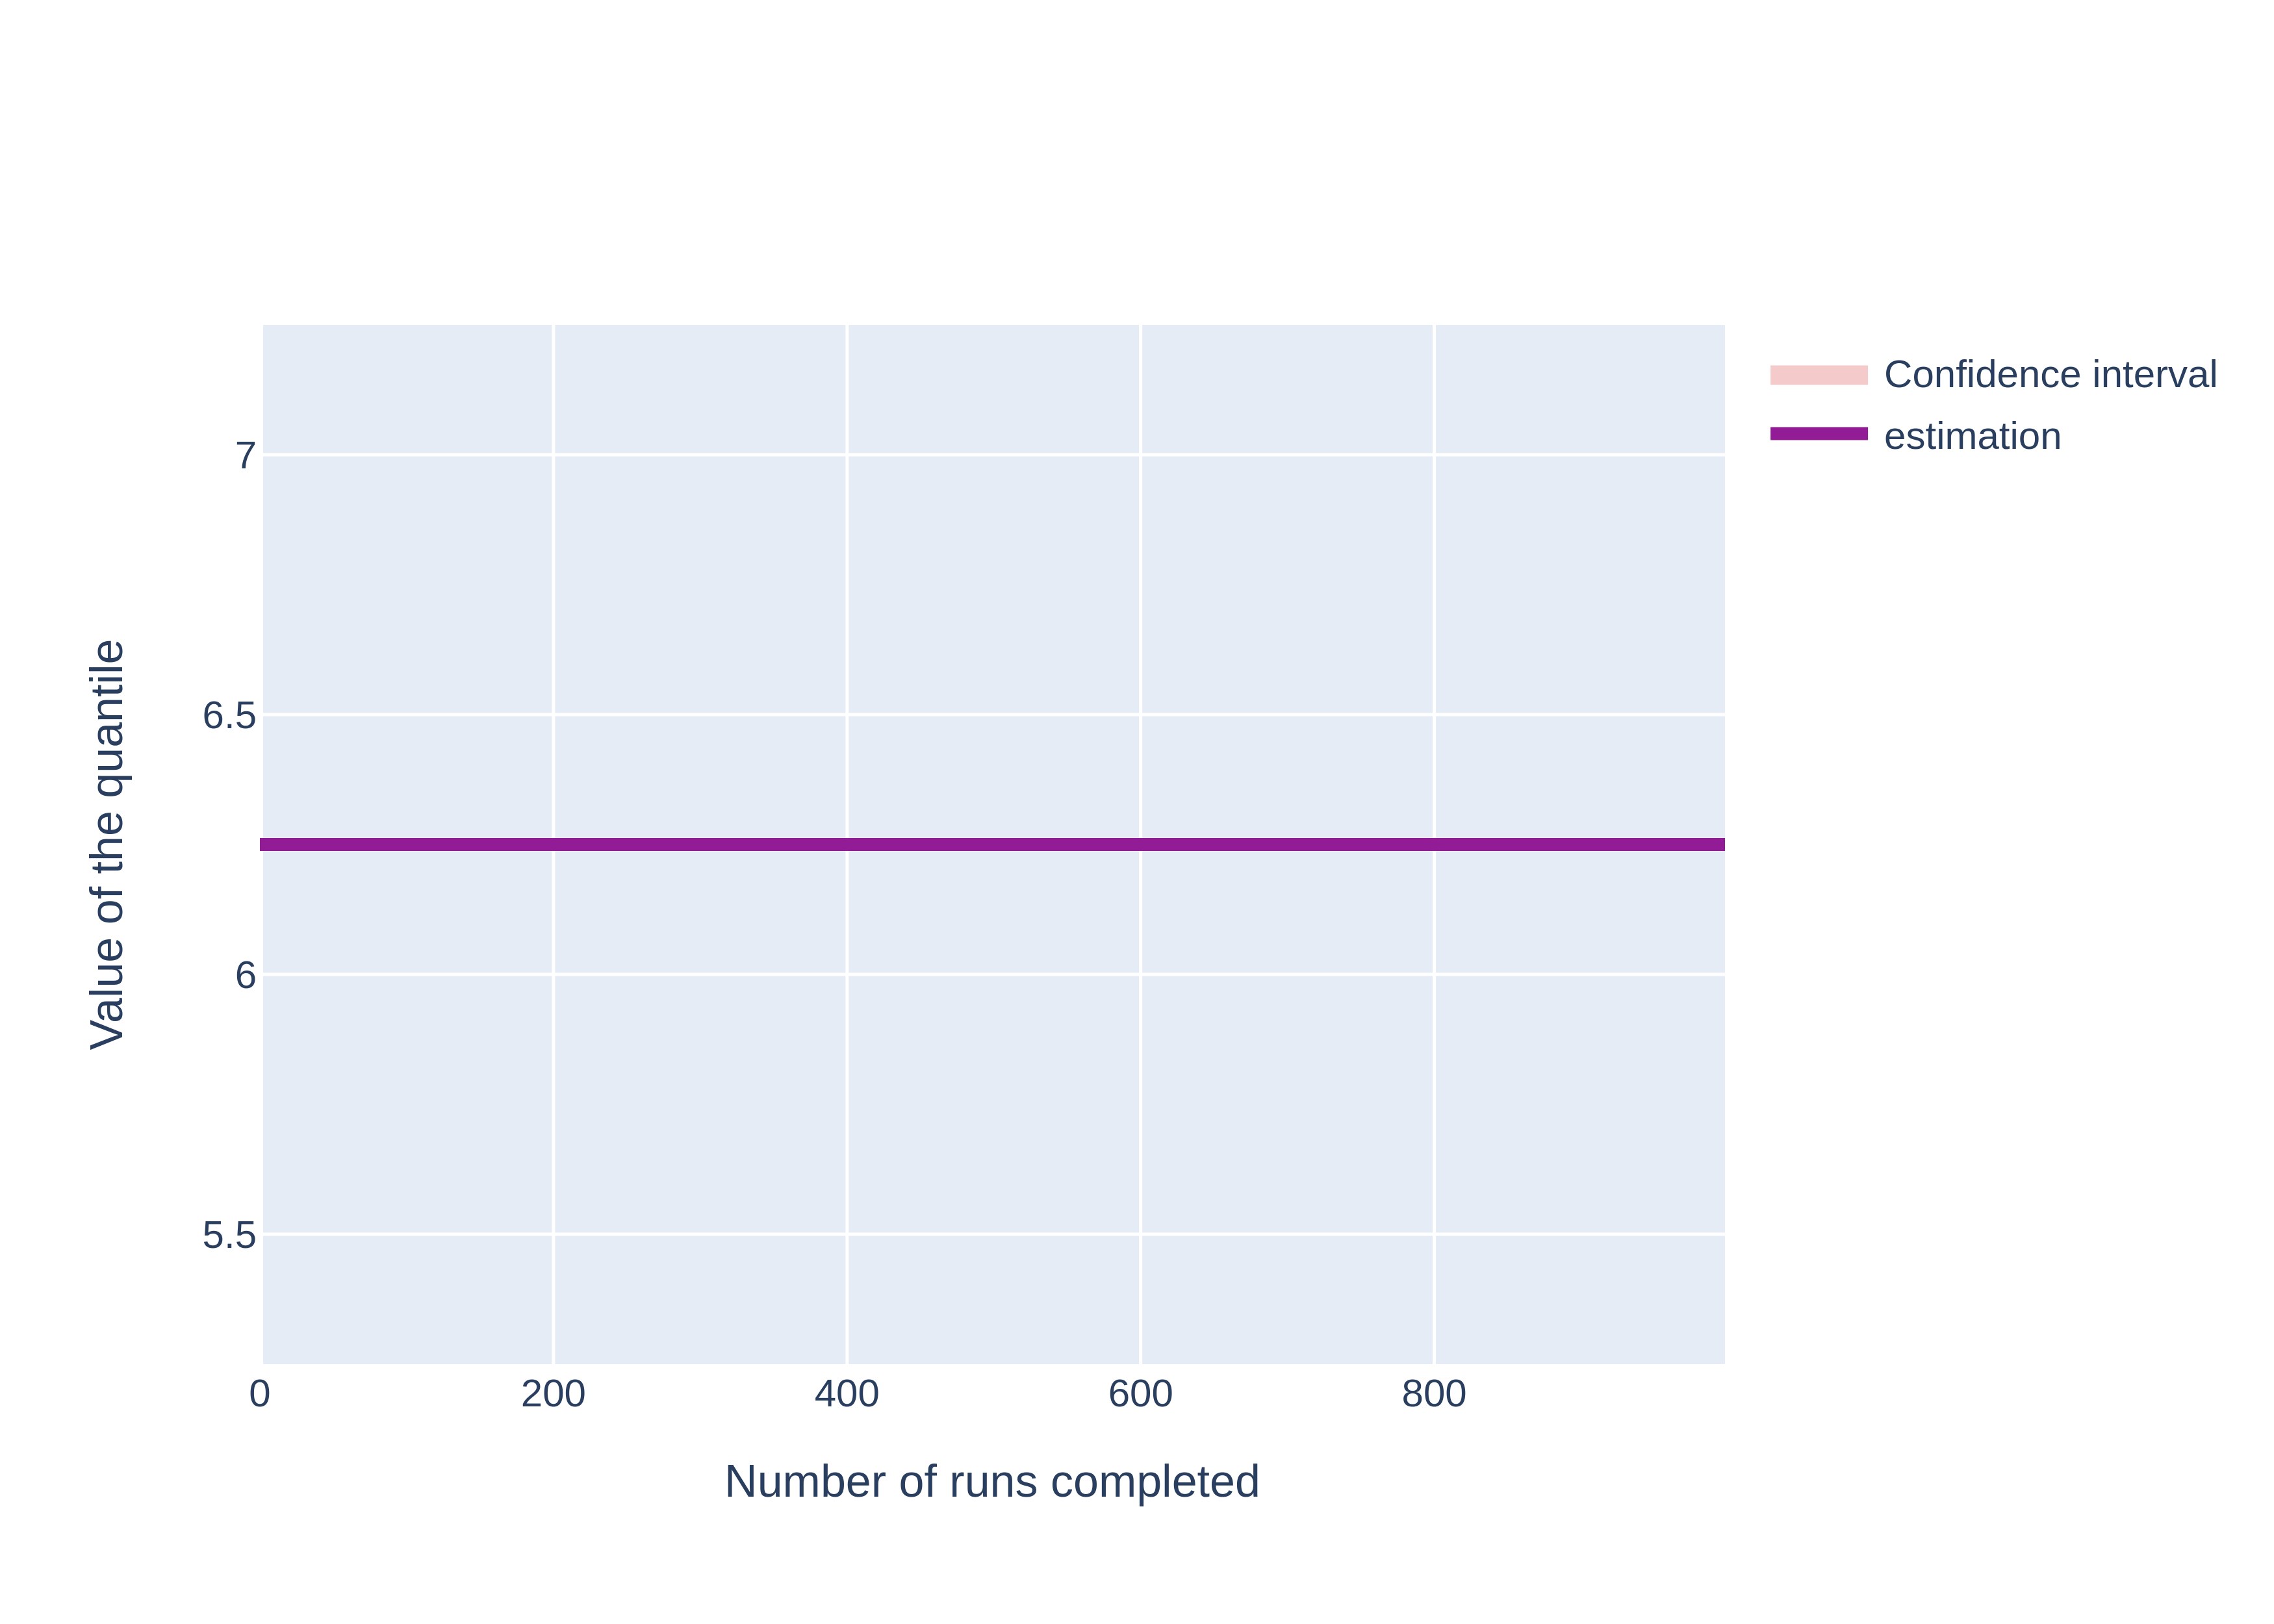
\includegraphics[width=\textwidth]{../fig/quantile4/TFTP4 DAT_4mn.png}
        \caption{Simulation time: 4min}
        \vspace{.5cm}
    \end{subfigure}
    \begin{subfigure}{.495\textwidth}
        \centering
        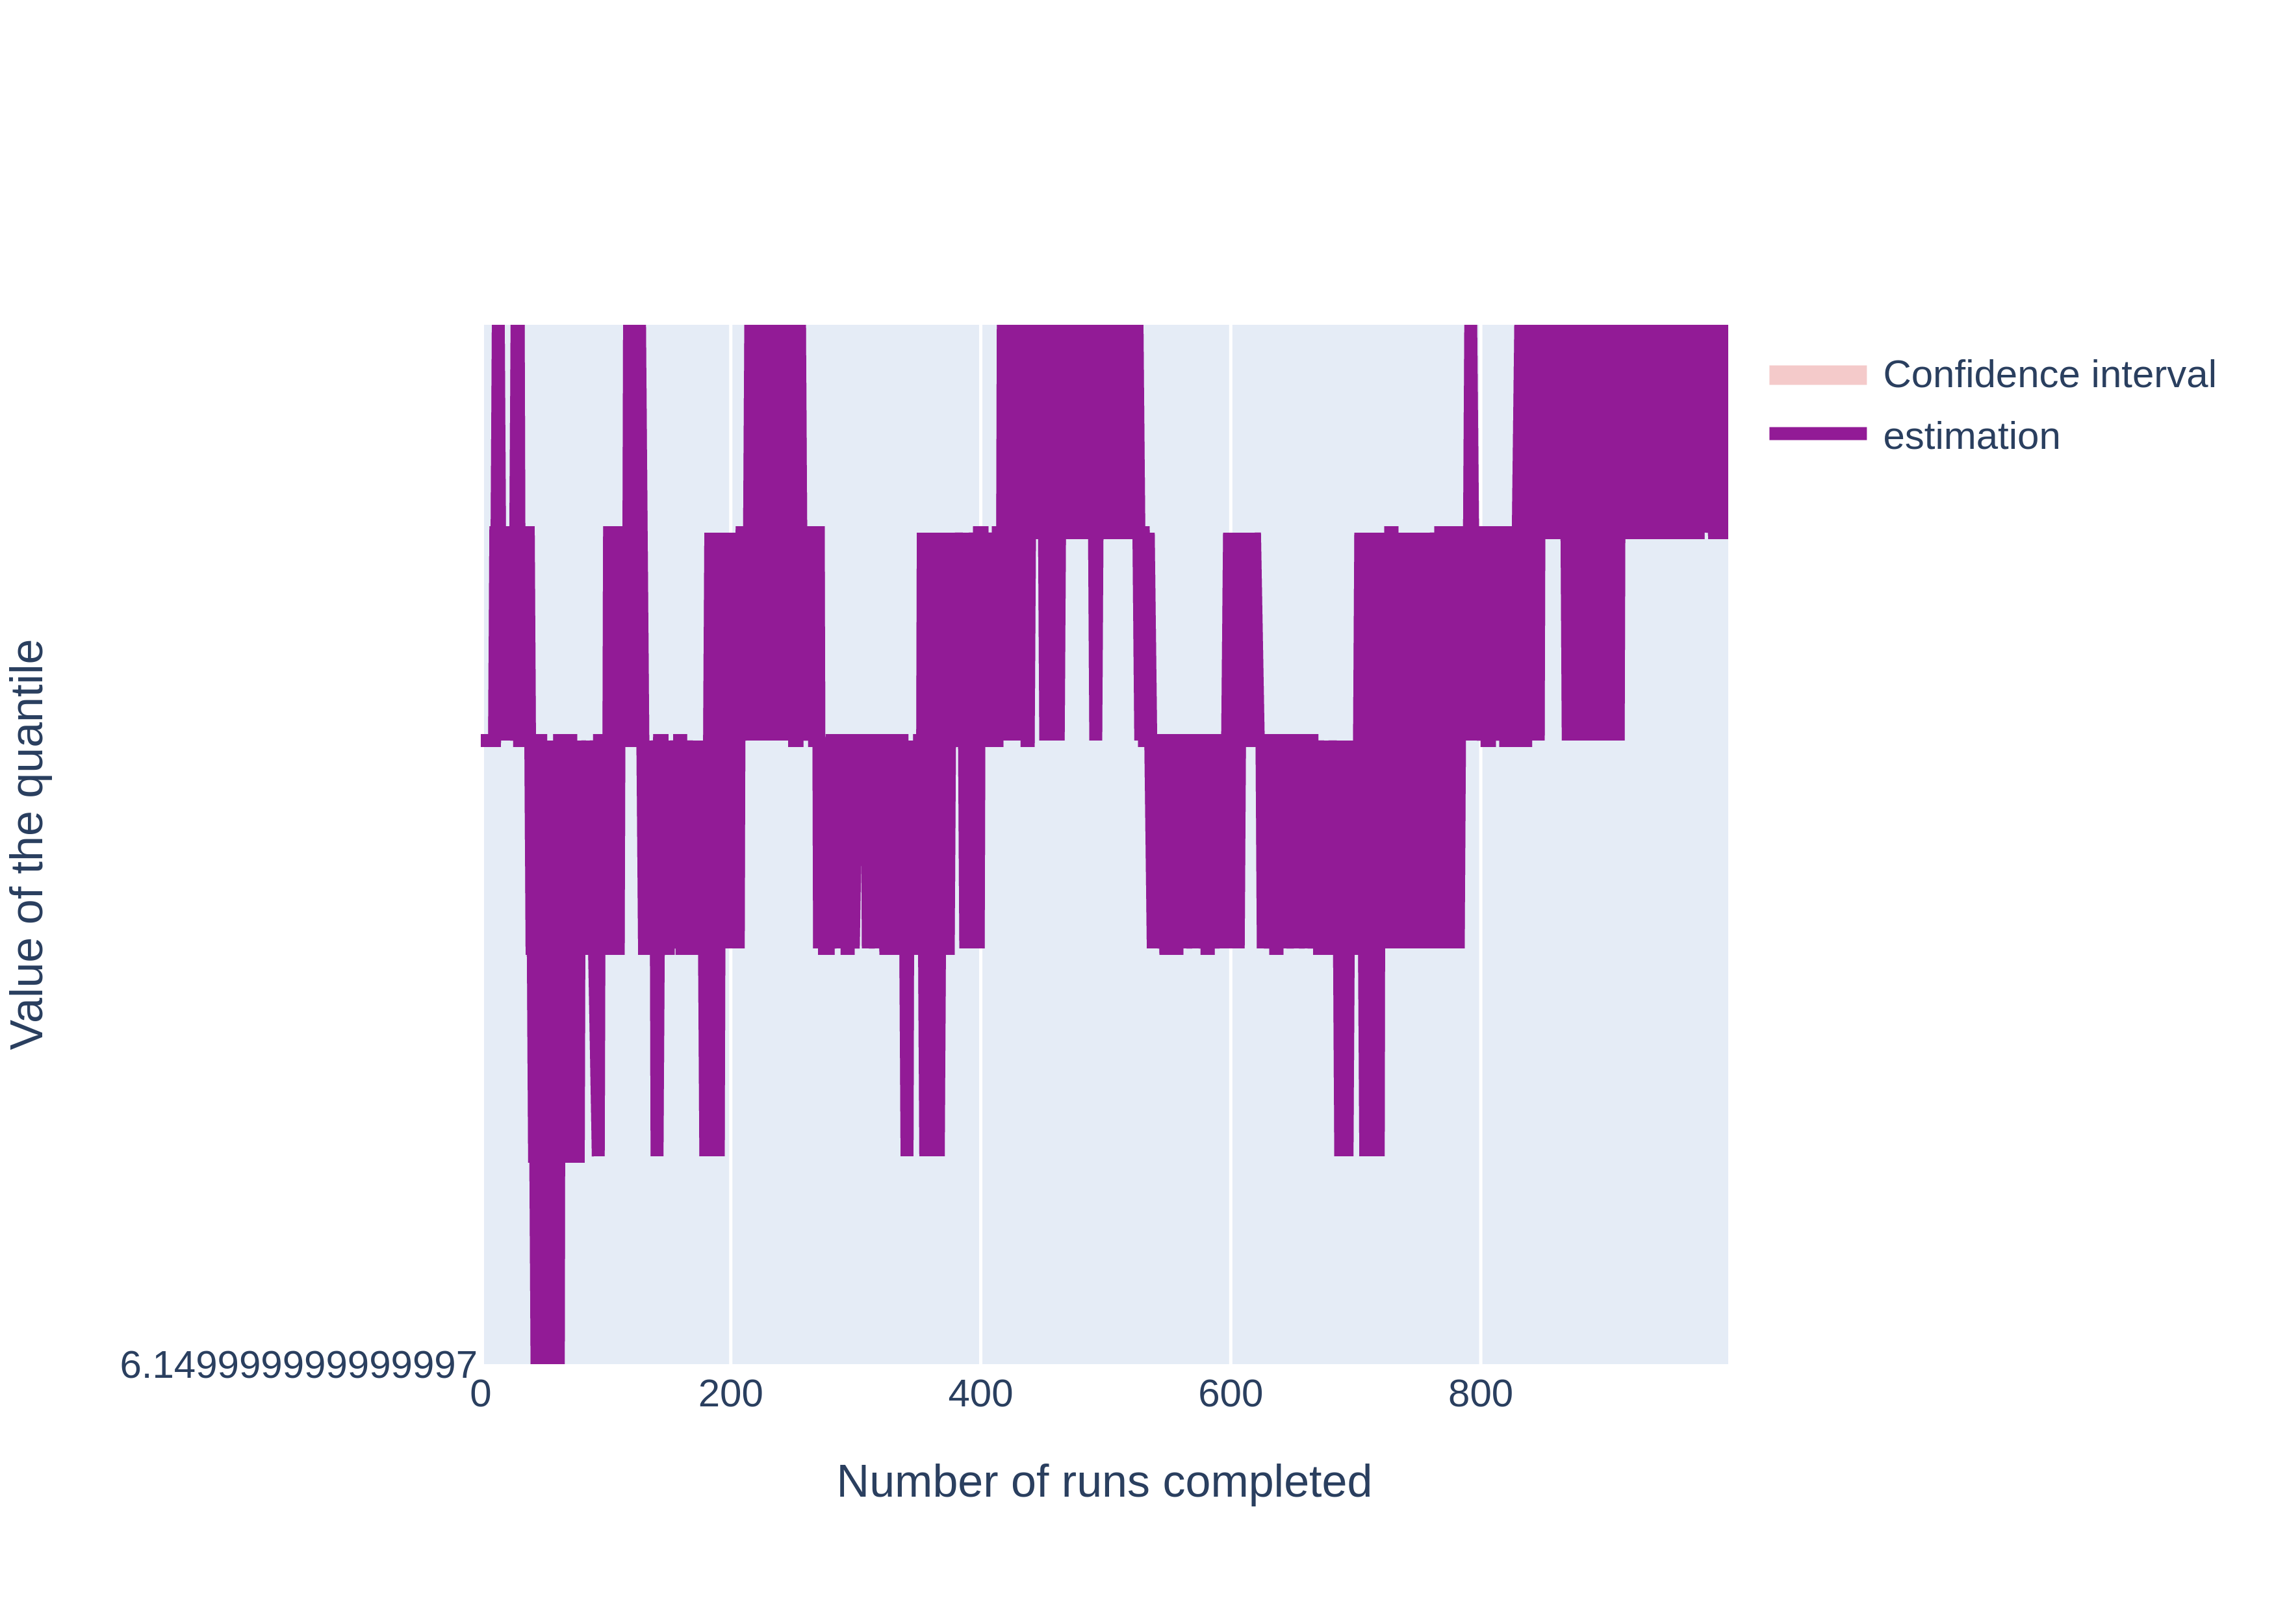
\includegraphics[width=\textwidth]{../fig/quantile4/TFTP4 DAT_40mn.png}
        \caption{Simulation time: 40min}
    \end{subfigure}
    \begin{subfigure}{.495\textwidth}
        \centering
        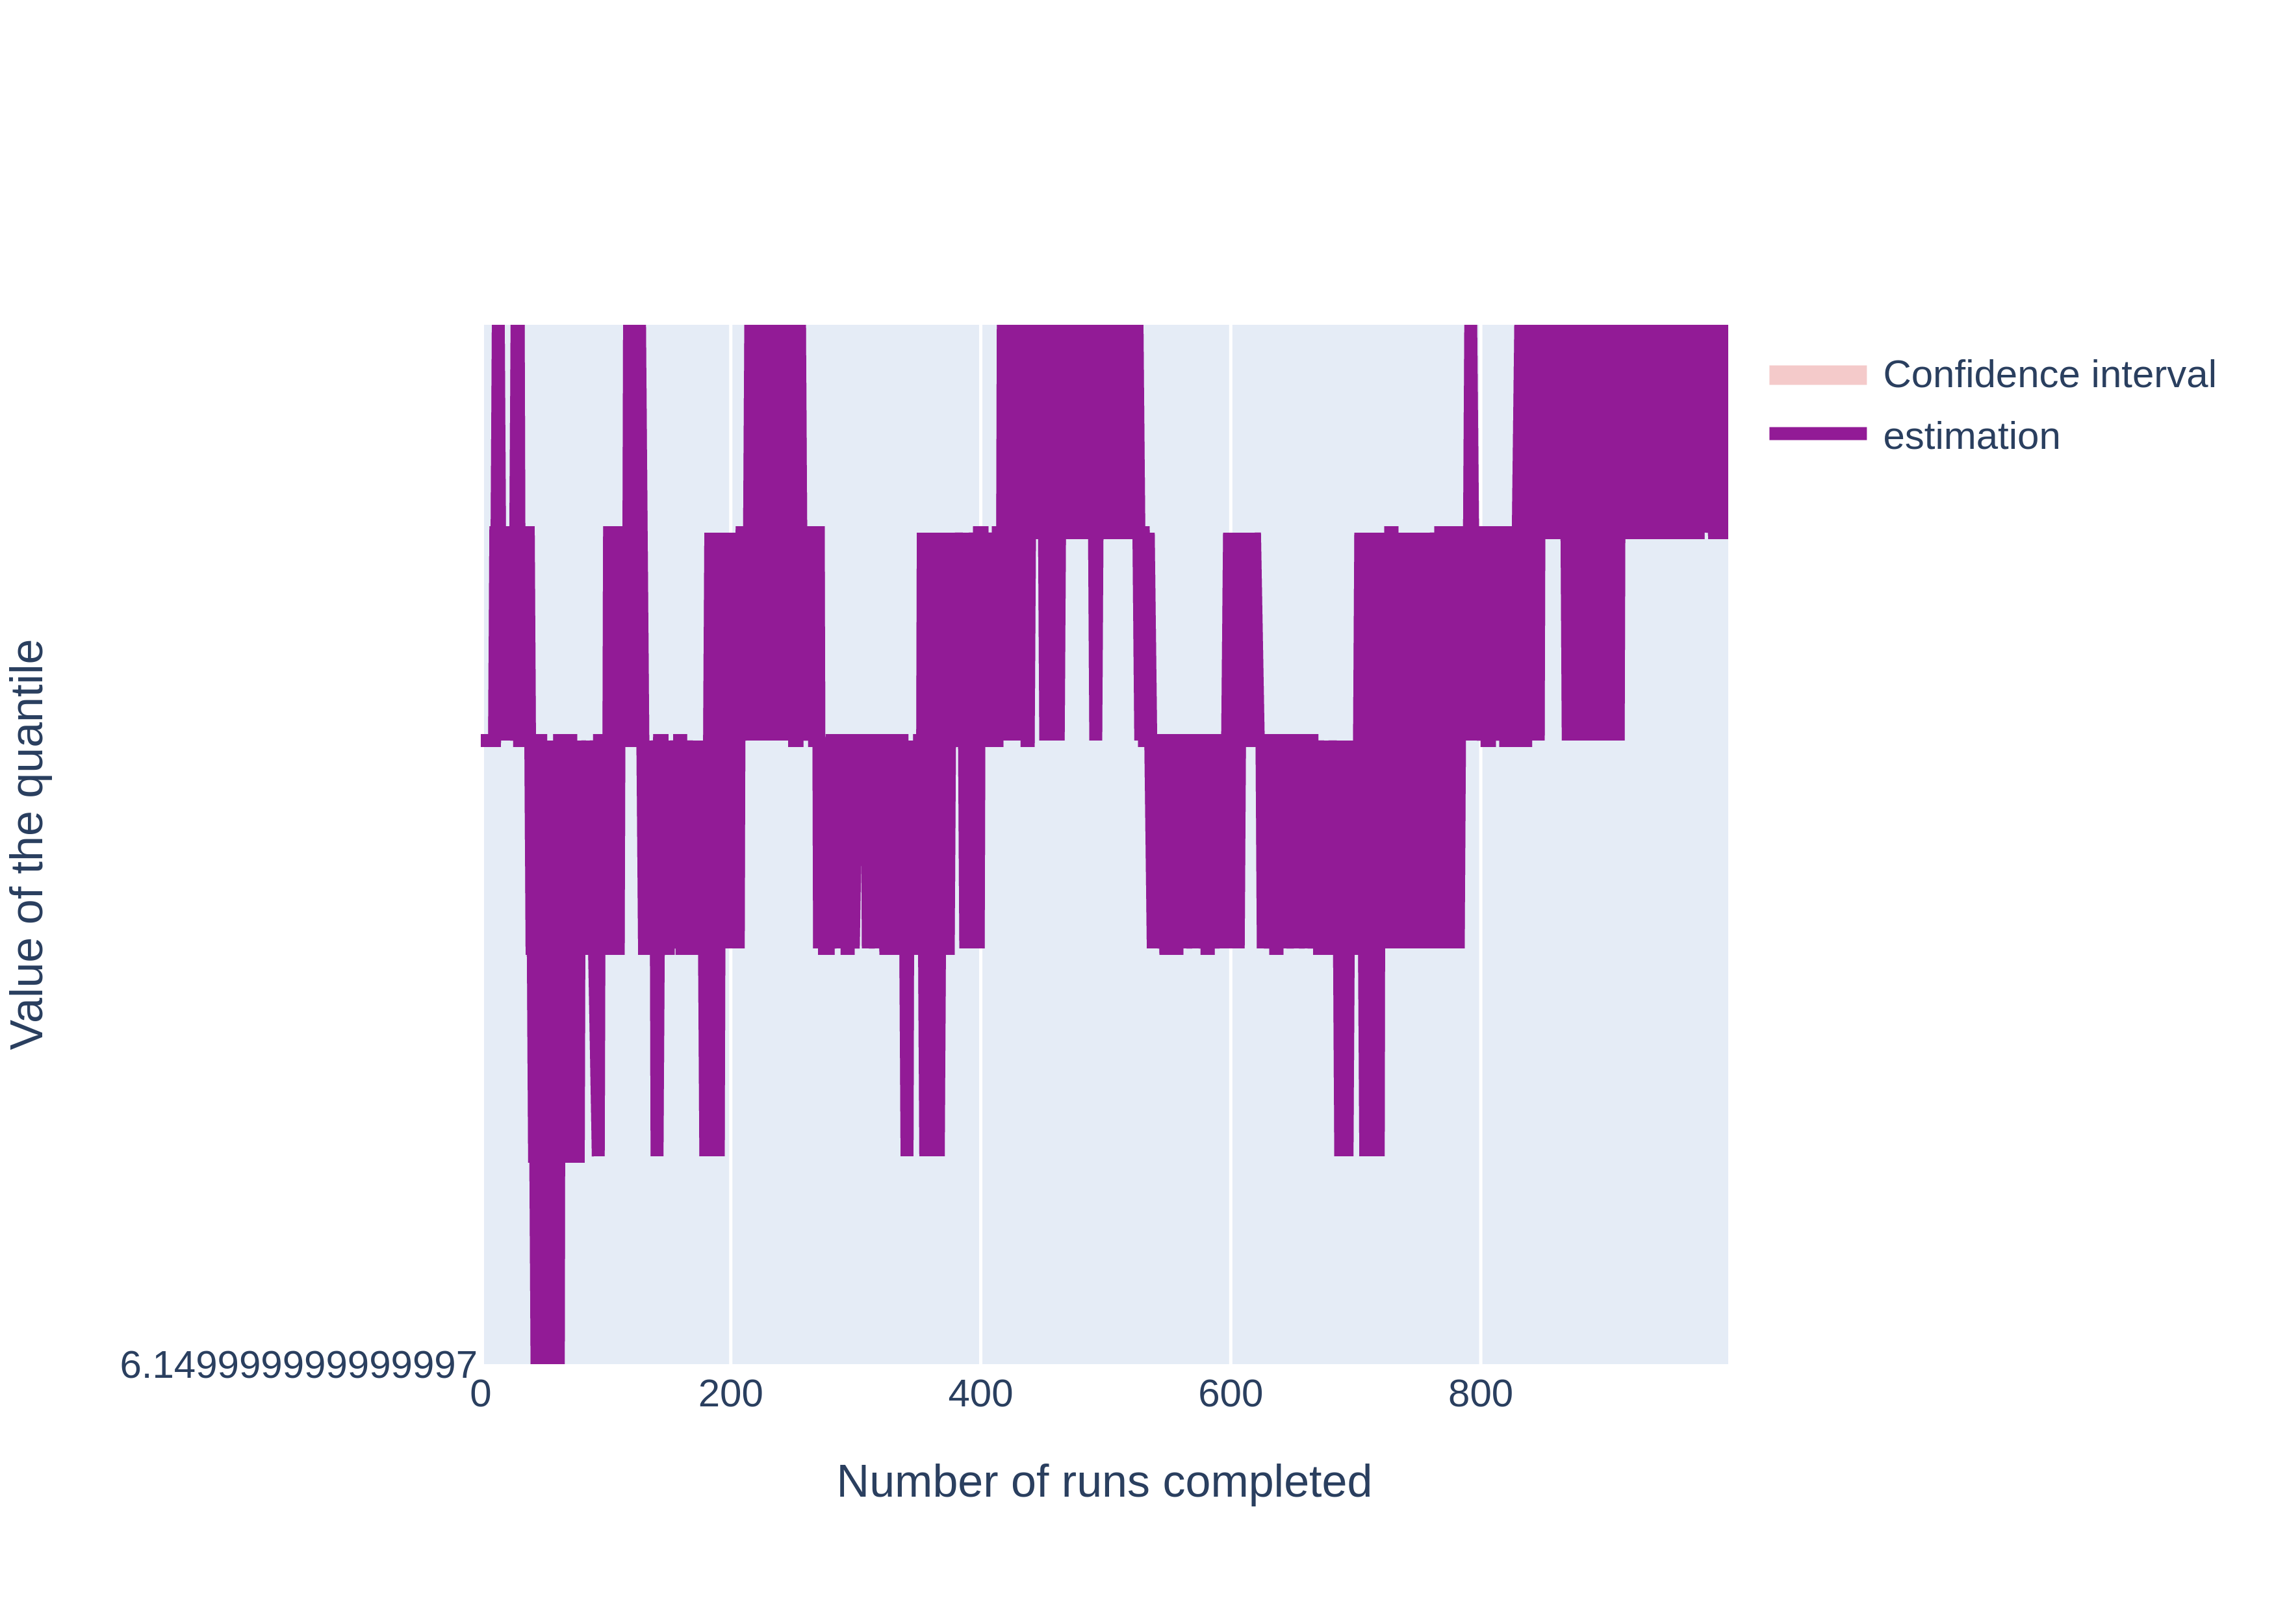
\includegraphics[width=\textwidth]{../fig/quantile4/TFTP4 DAT_400mn.png}
        \caption{Simulation time: 400min}
    \end{subfigure}
    \caption{TFTP4 DAT $q_4$ after multiple simulation times}
\end{figure}

\subsubsection{Quantile 5}
\begin{figure}[H]
    \centering
    \begin{subfigure}{.495\textwidth}
        \centering
        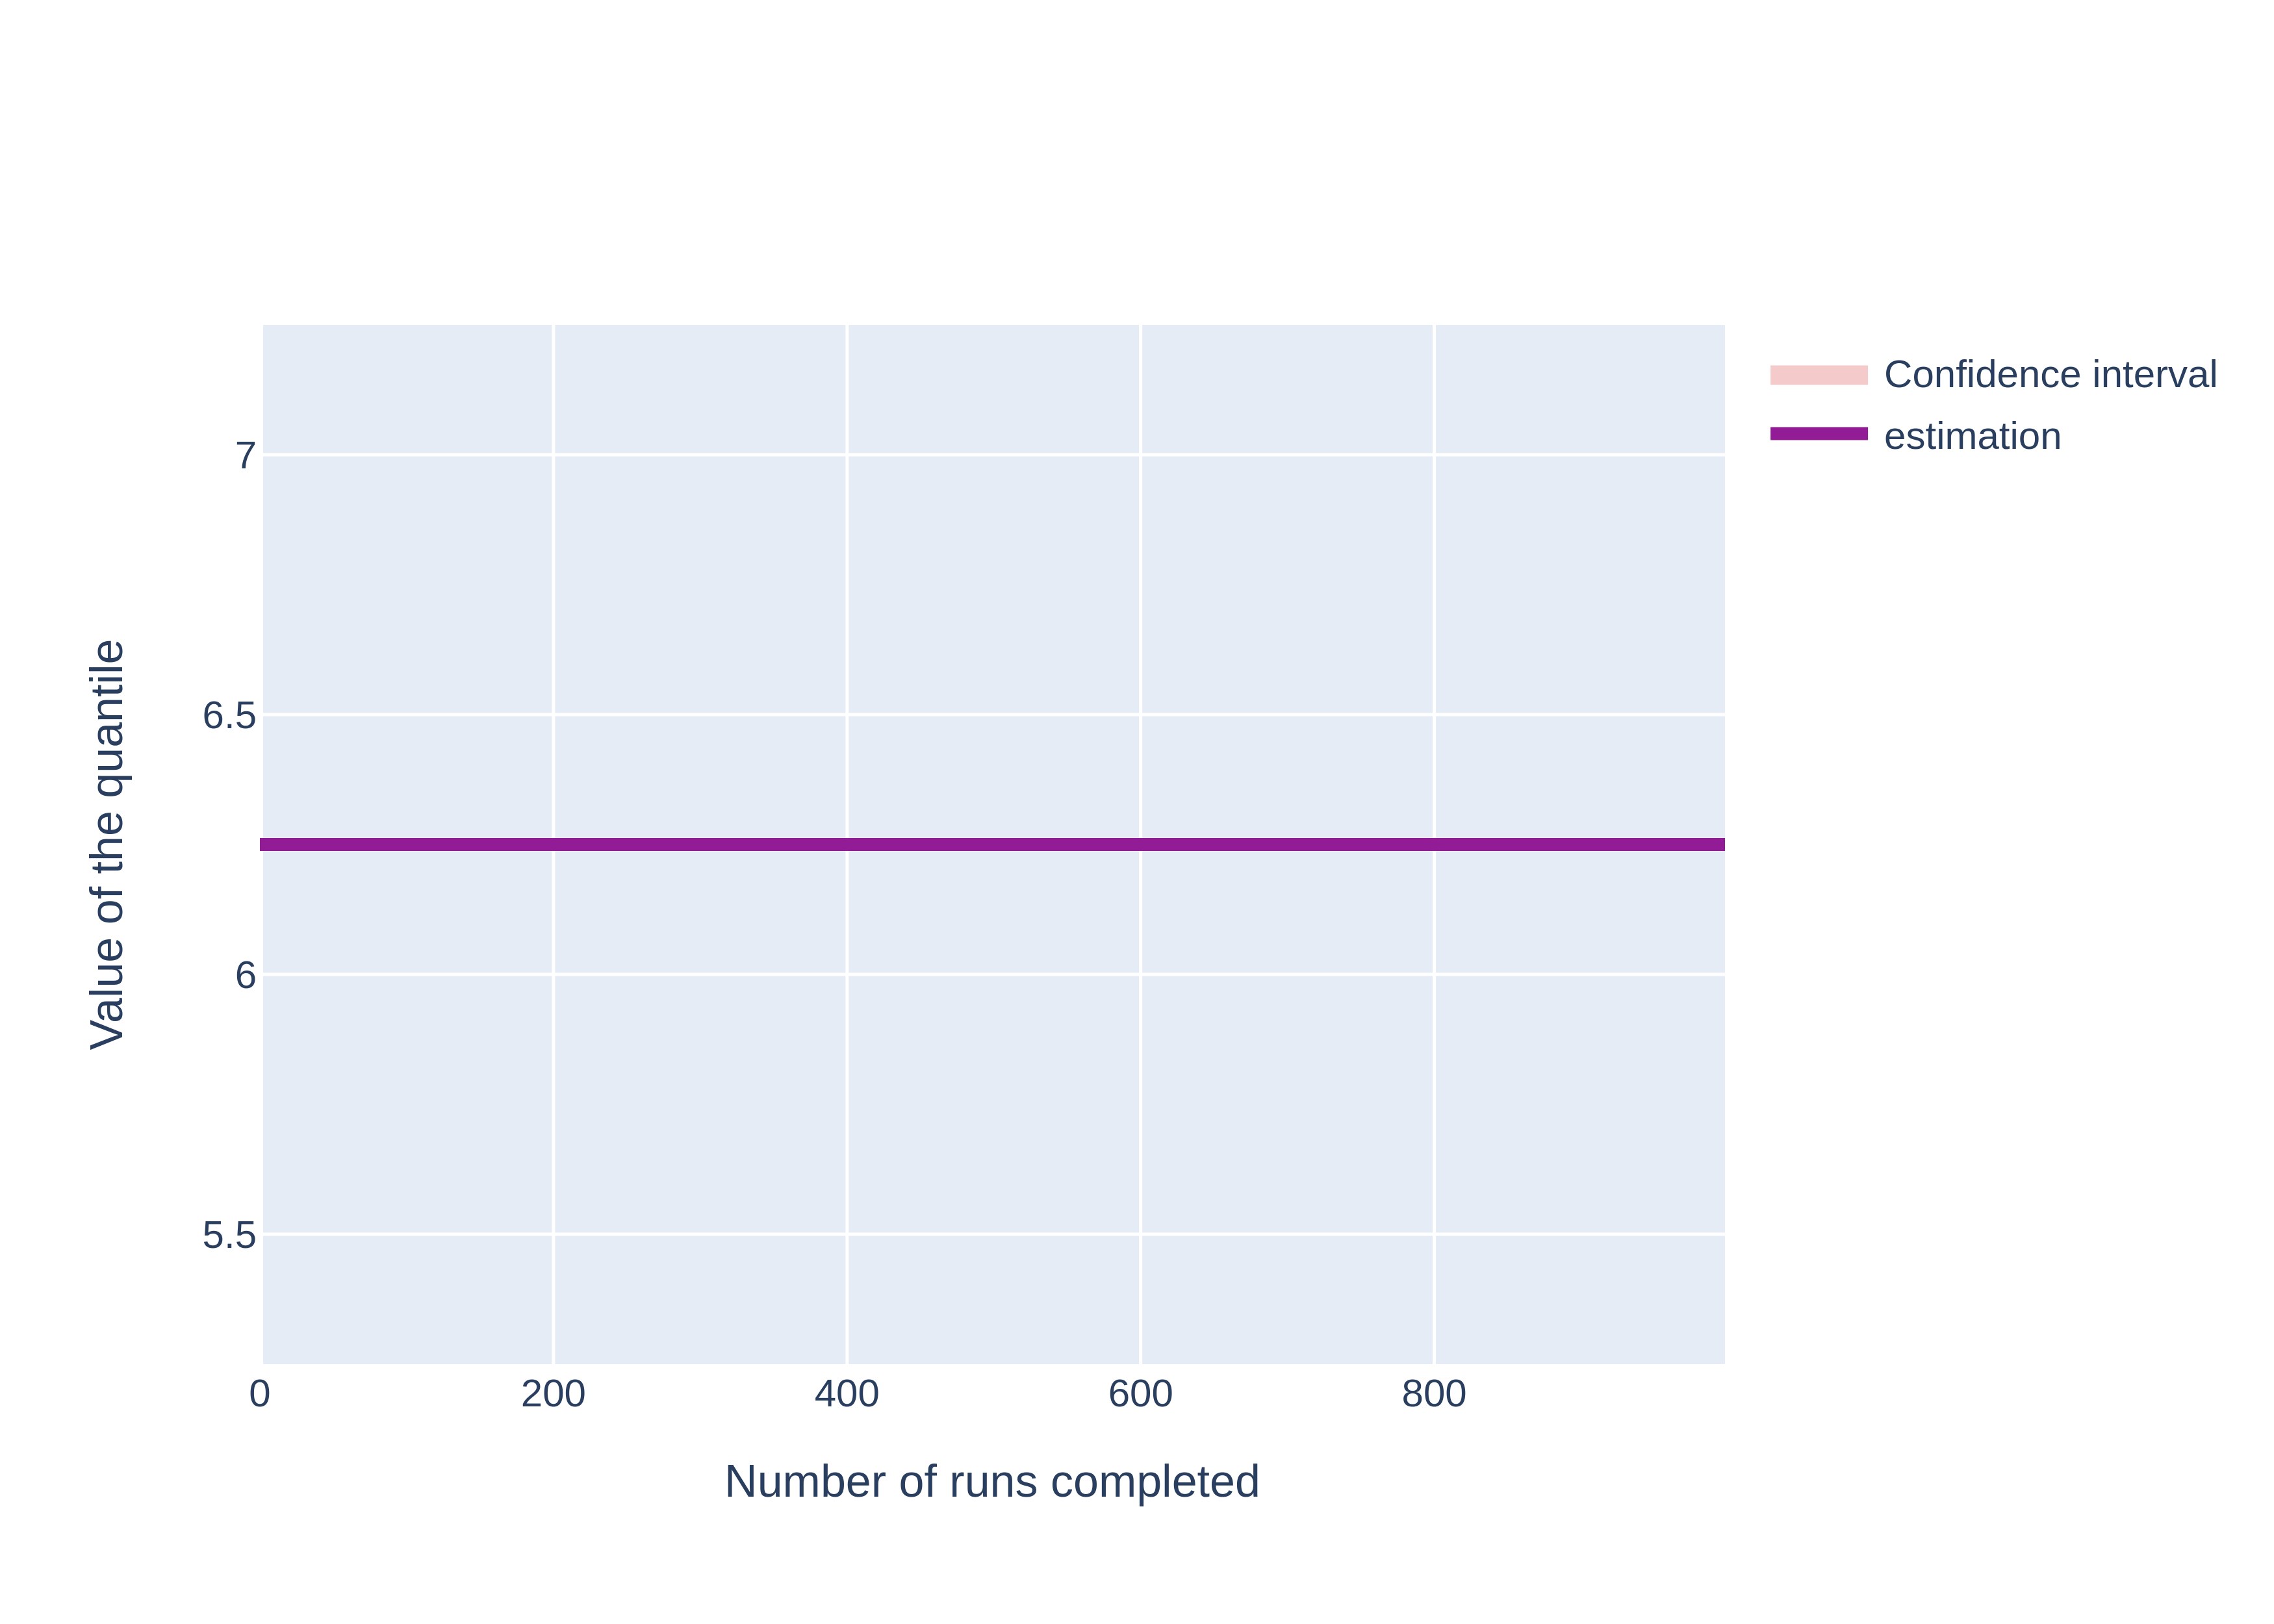
\includegraphics[width=\textwidth]{../fig/quantile5/TFTP4_DAT_24s.png}
        \caption{Simulation time: 24s}
        \vspace{.5cm}
    \end{subfigure}
    \begin{subfigure}{.495\textwidth}
        \centering
        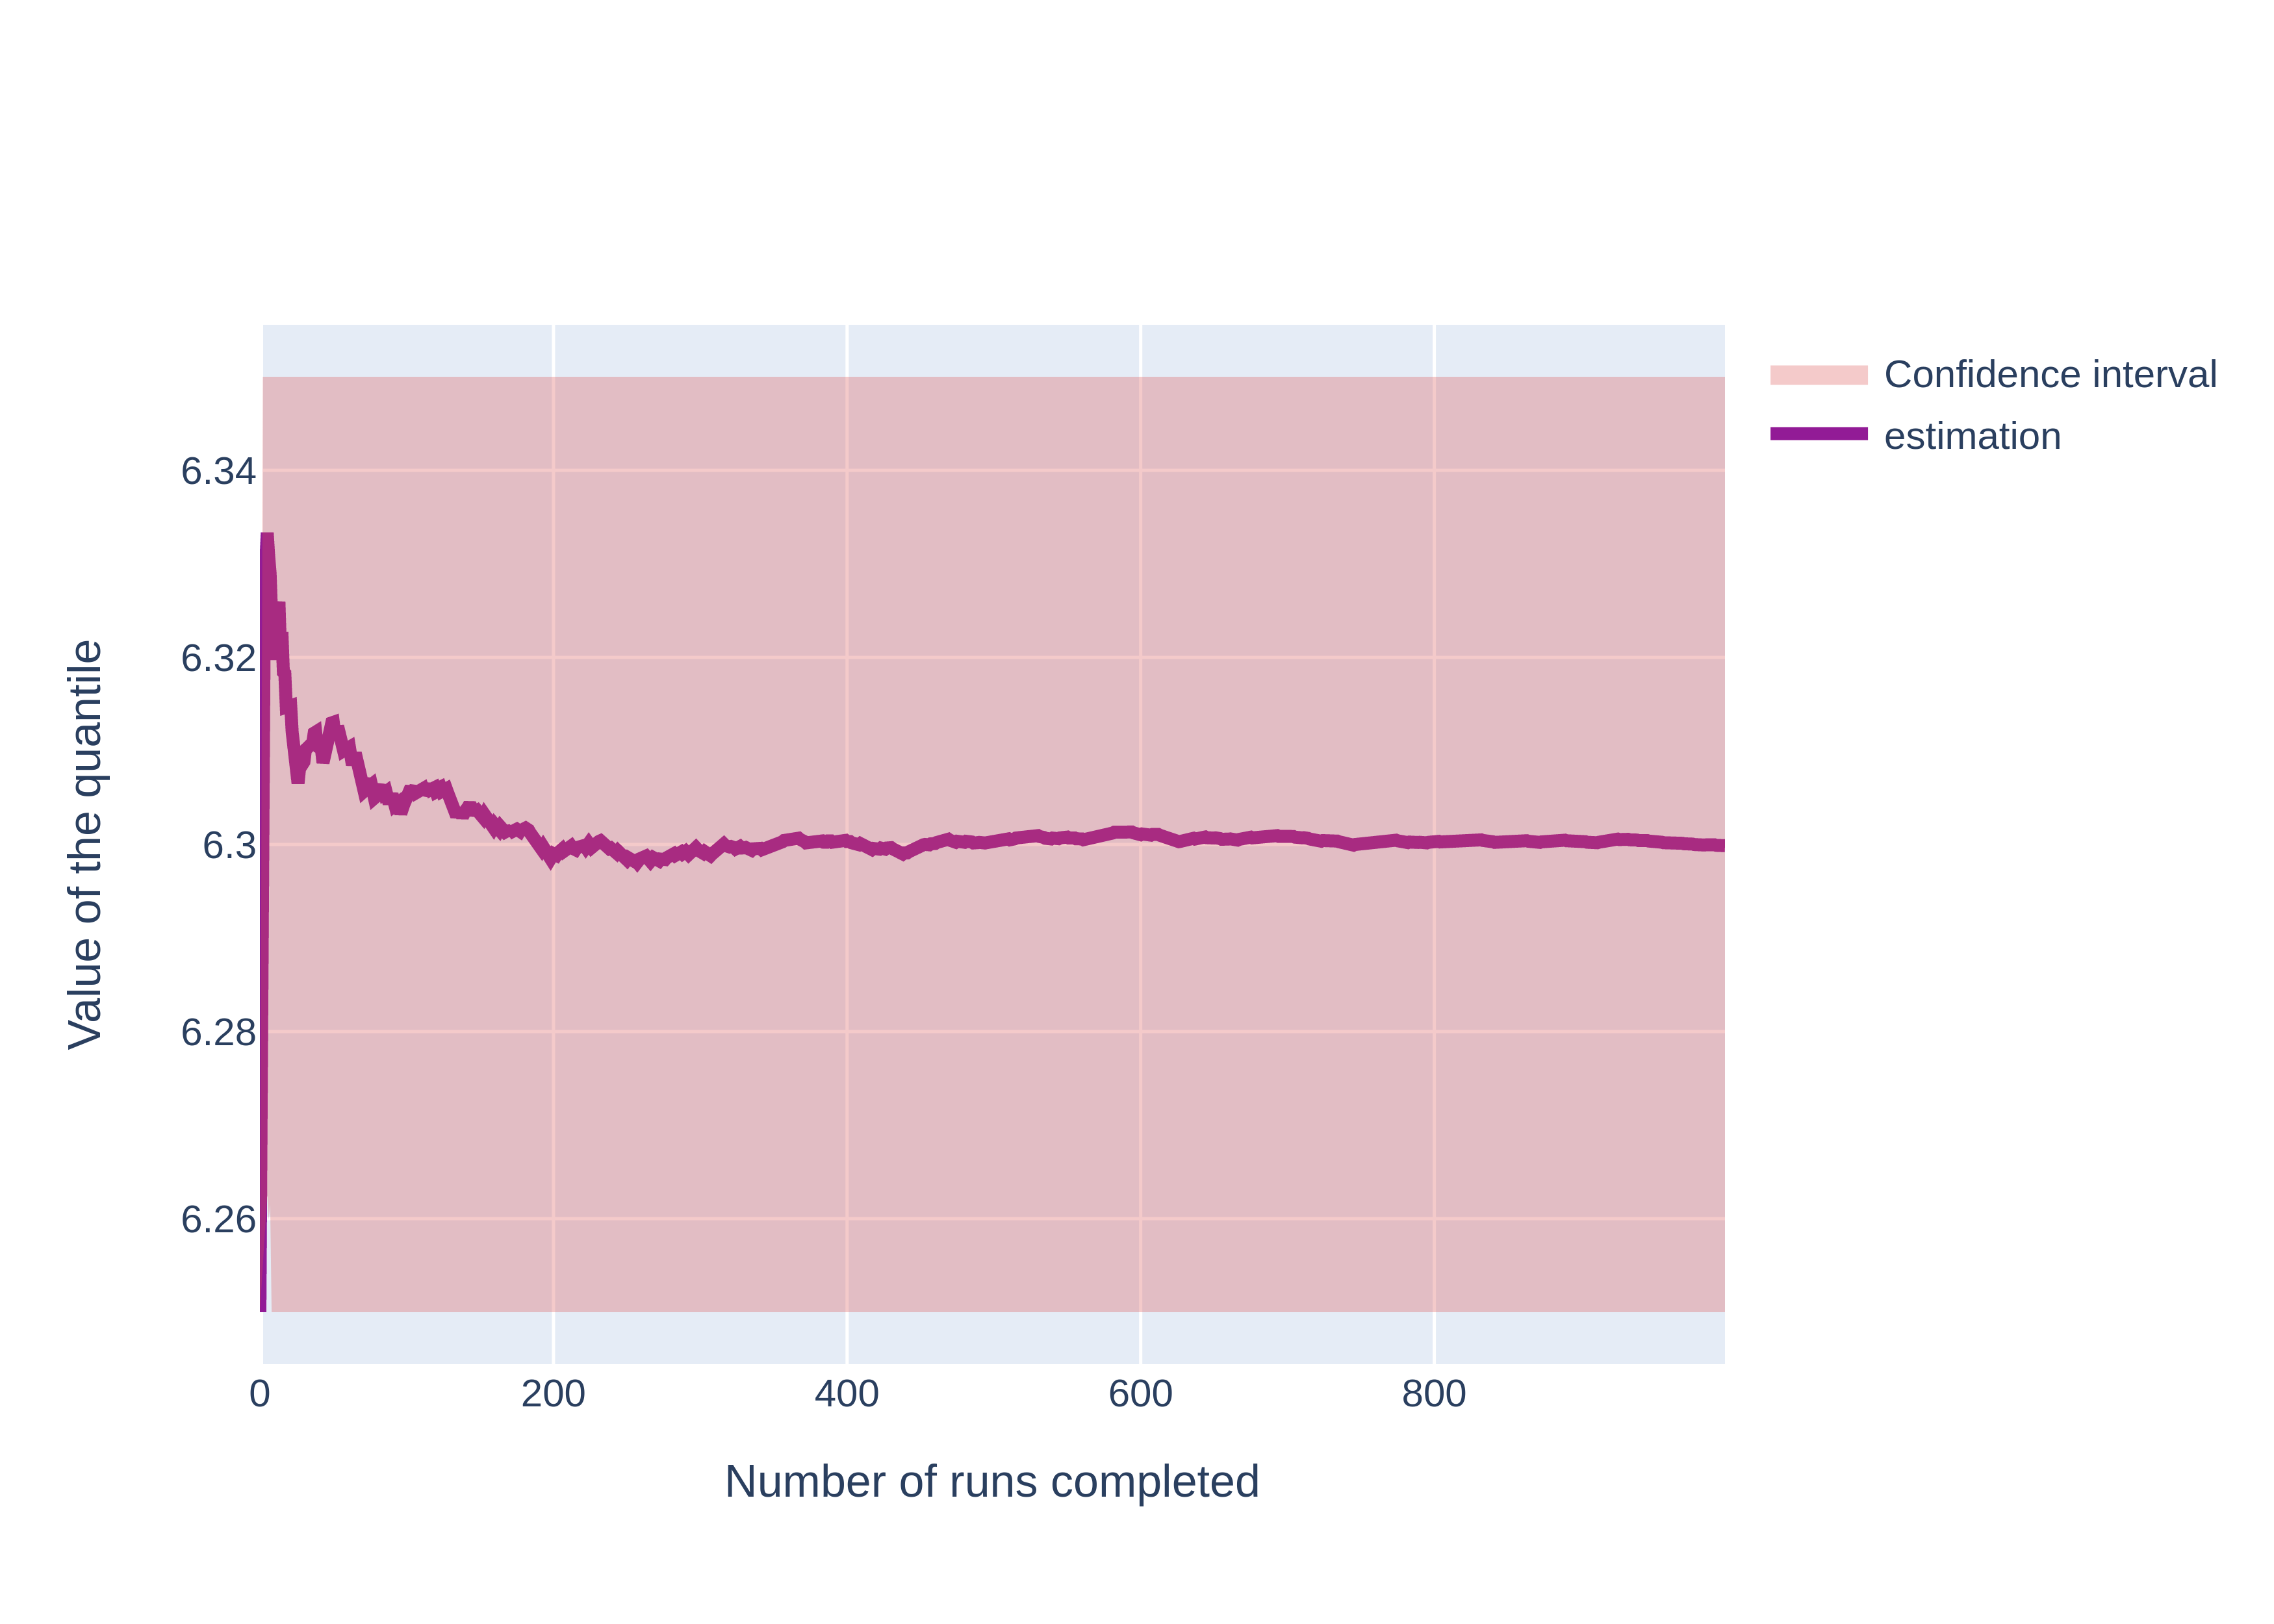
\includegraphics[width=\textwidth]{../fig/quantile5/TFTP4 DAT_4mn.png}
        \caption{Simulation time: 4min}
        \vspace{.5cm}
    \end{subfigure}
    \begin{subfigure}{.495\textwidth}
        \centering
        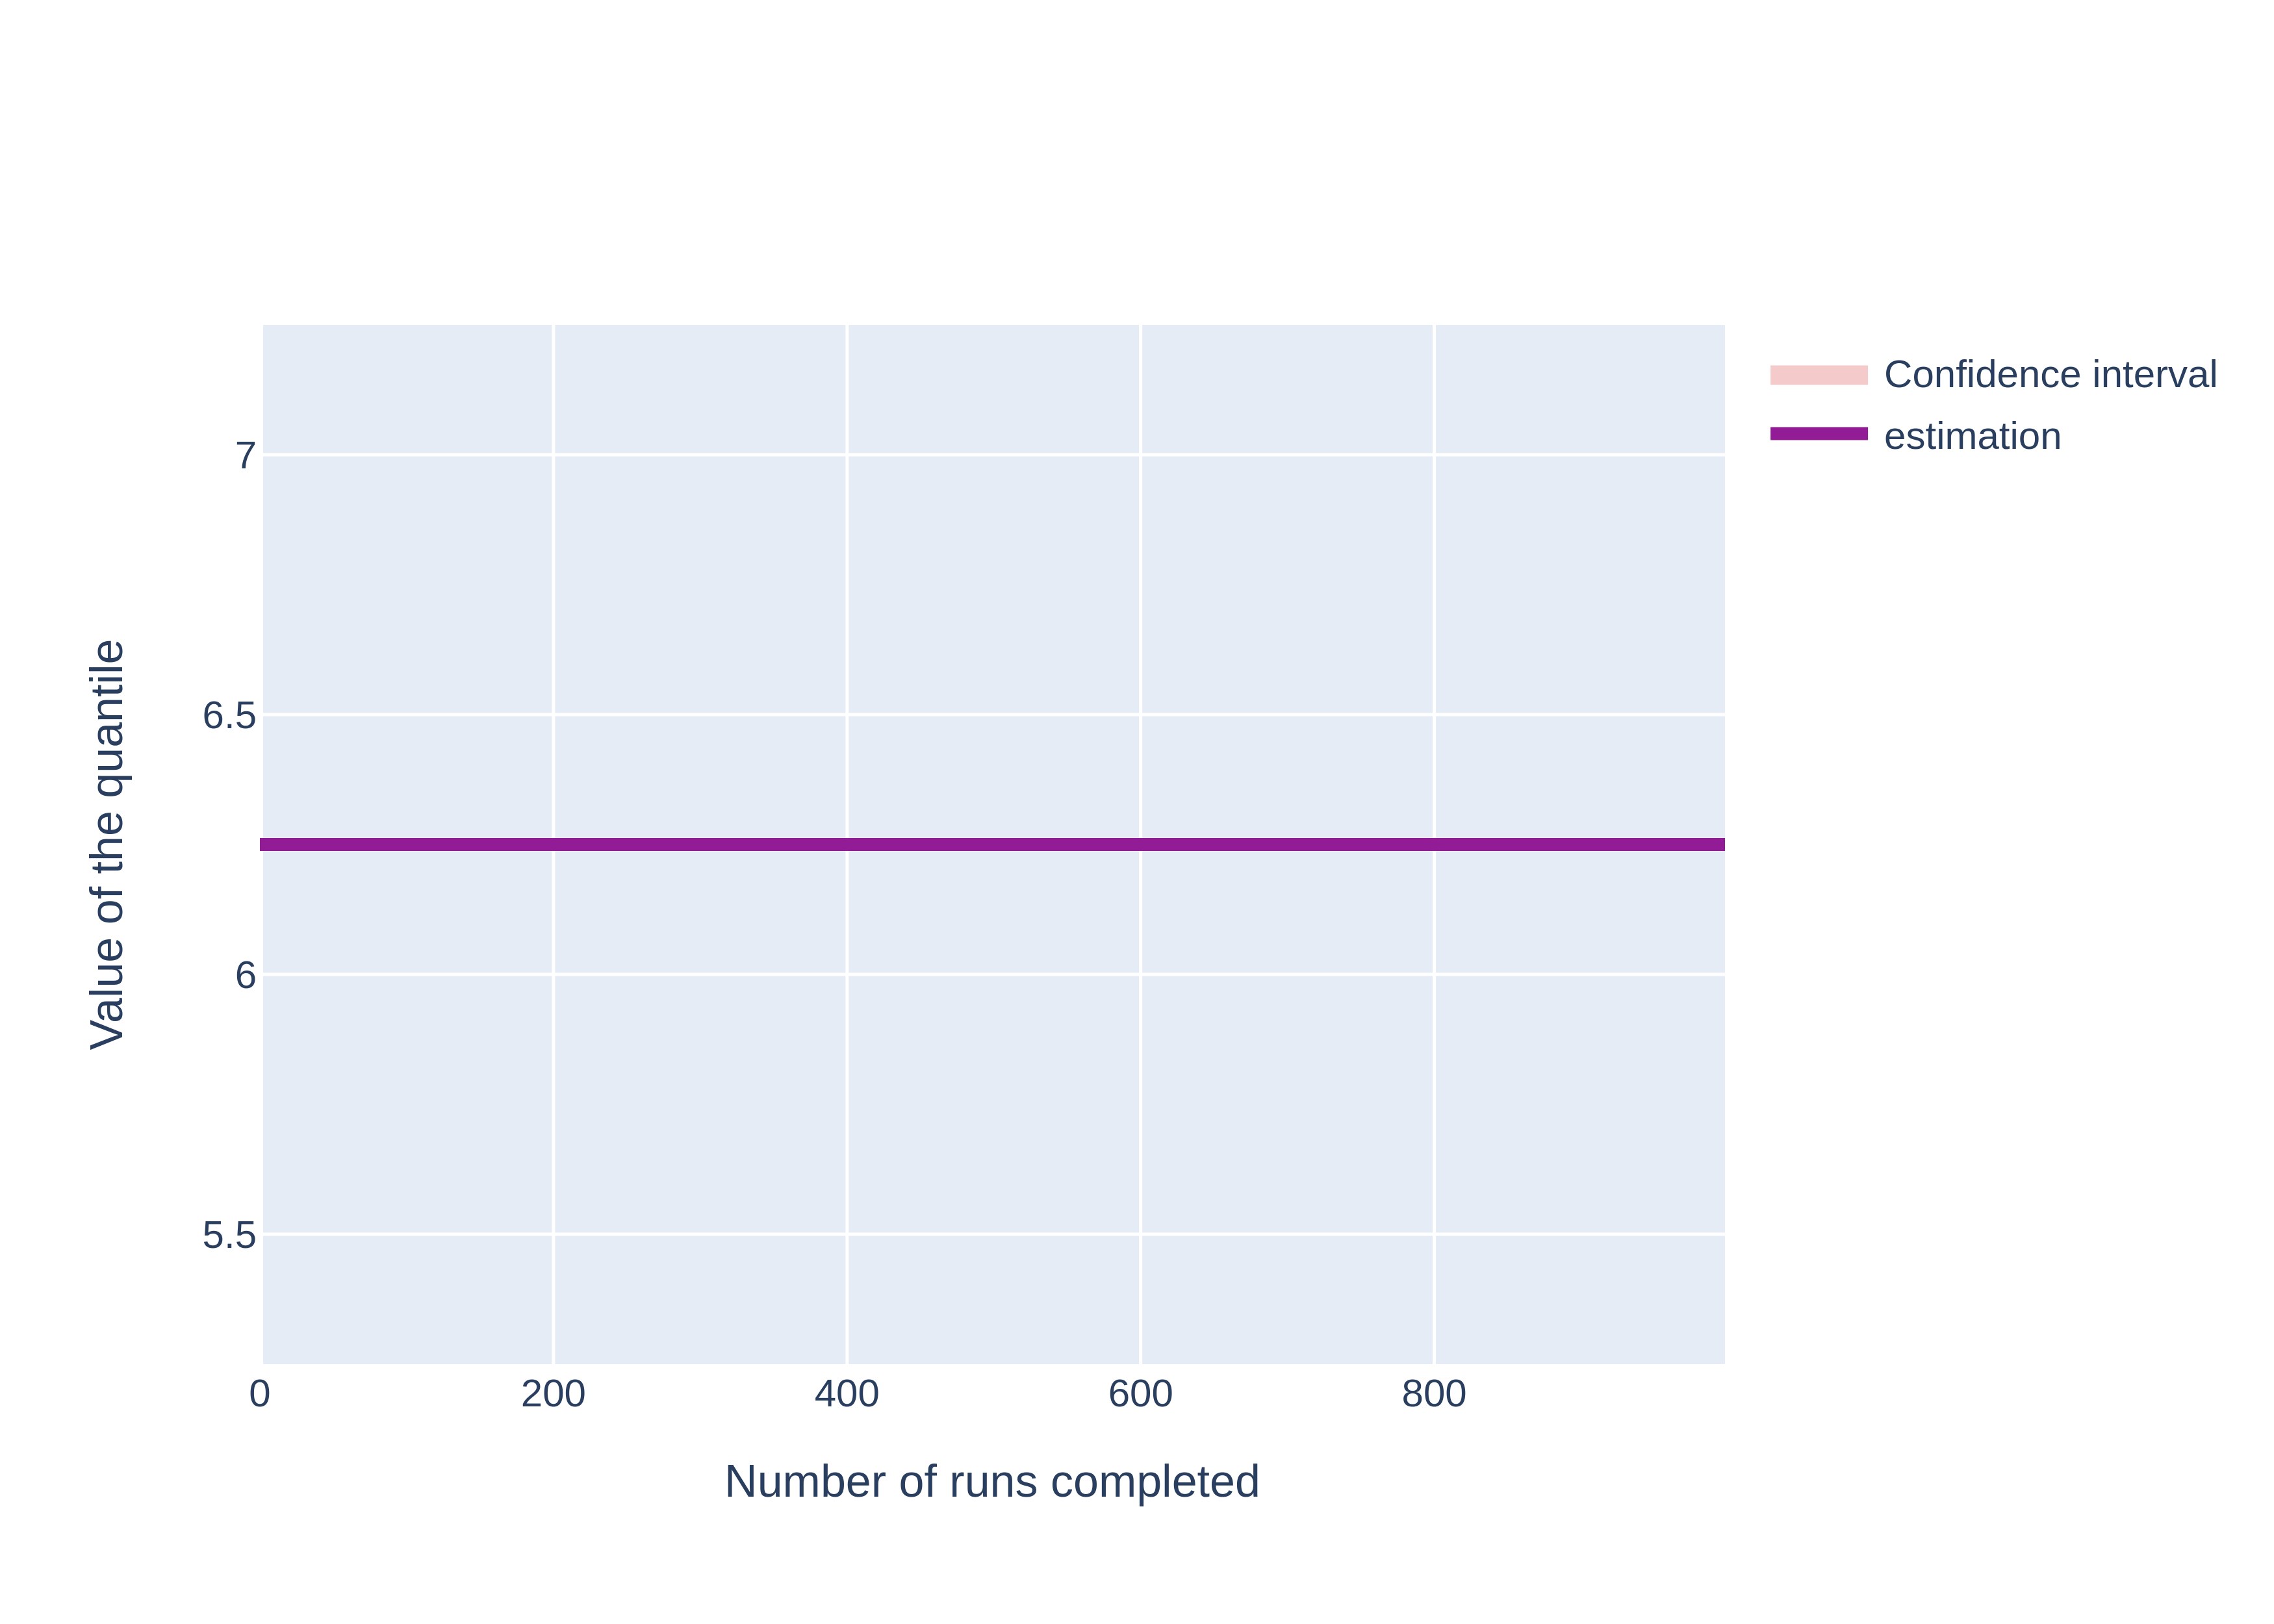
\includegraphics[width=\textwidth]{../fig/quantile5/TFTP4 DAT_40mn.png}
        \caption{Simulation time: 40min}
    \end{subfigure}
    \begin{subfigure}{.495\textwidth}
        \centering
        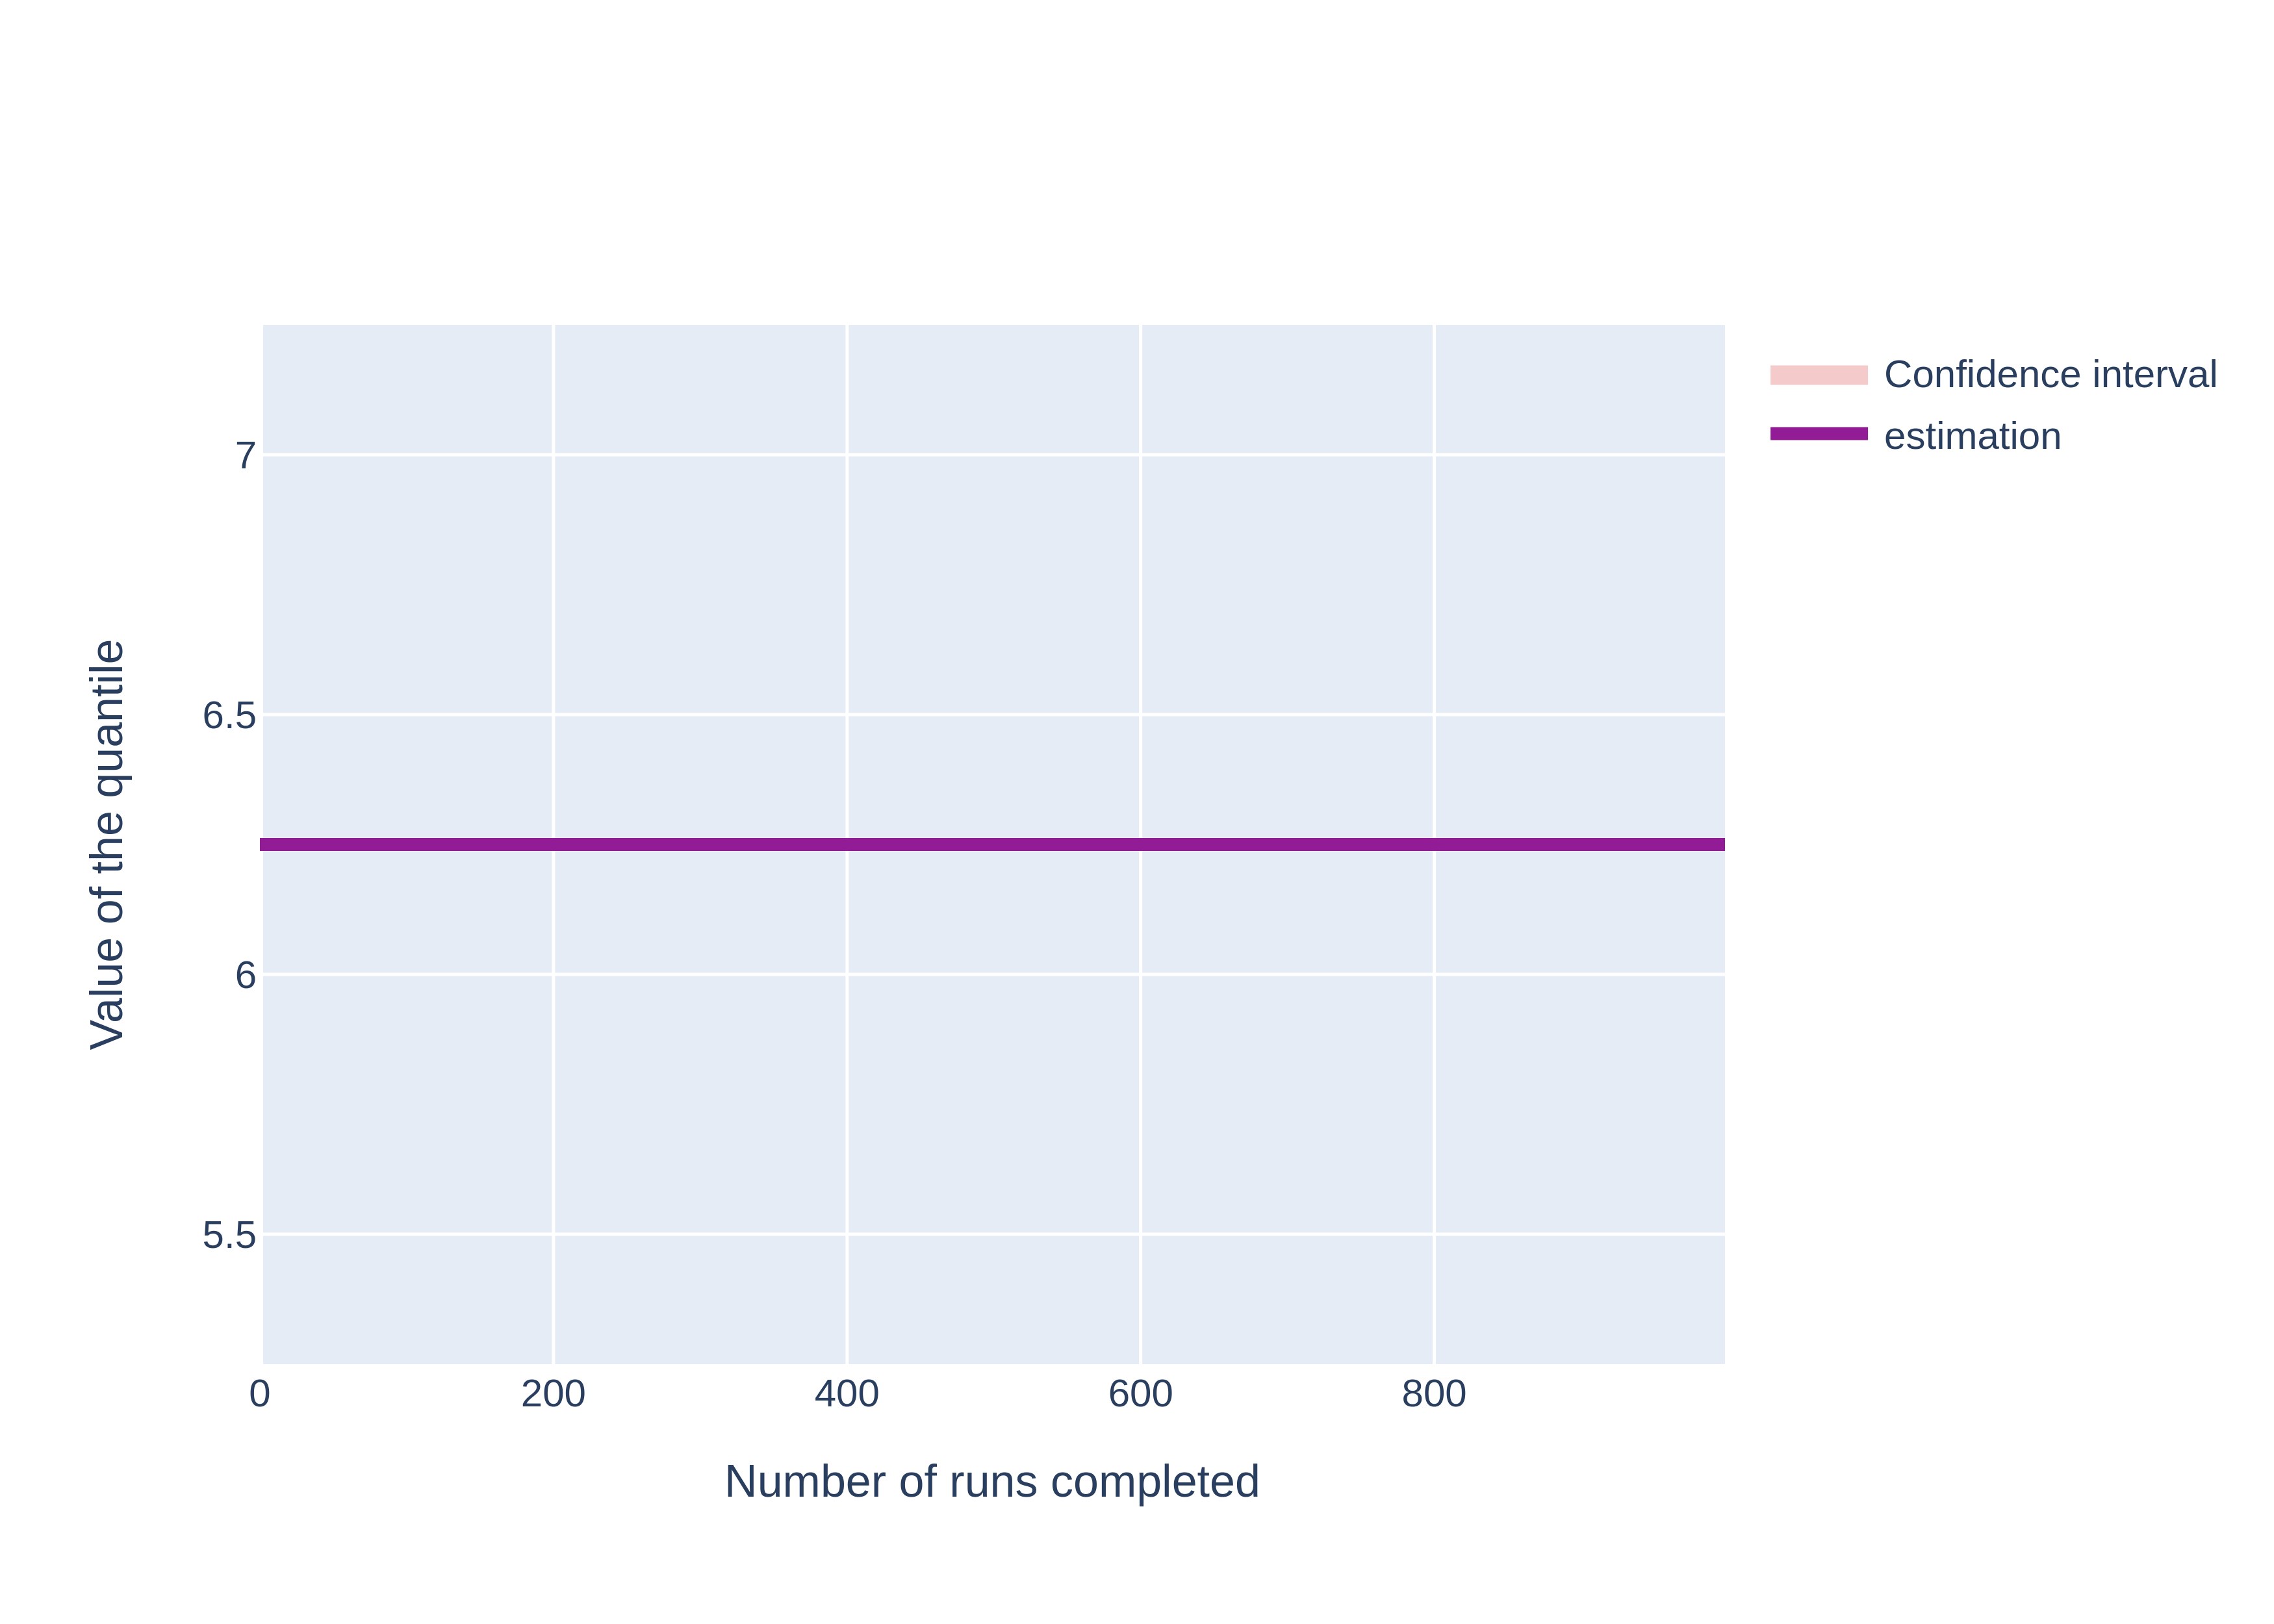
\includegraphics[width=\textwidth]{../fig/quantile5/TFTP4 DAT_400mn.png}
        \caption{Simulation time: 400min}
    \end{subfigure}
    \caption{TFTP4 DAT $q_5$ after multiple simulation times}
\end{figure}



\subsection{VD2}
\subsubsection{Data}

\begin{figure}[H]
    \centering
    \begin{subfigure}{.495\textwidth}
        \centering
        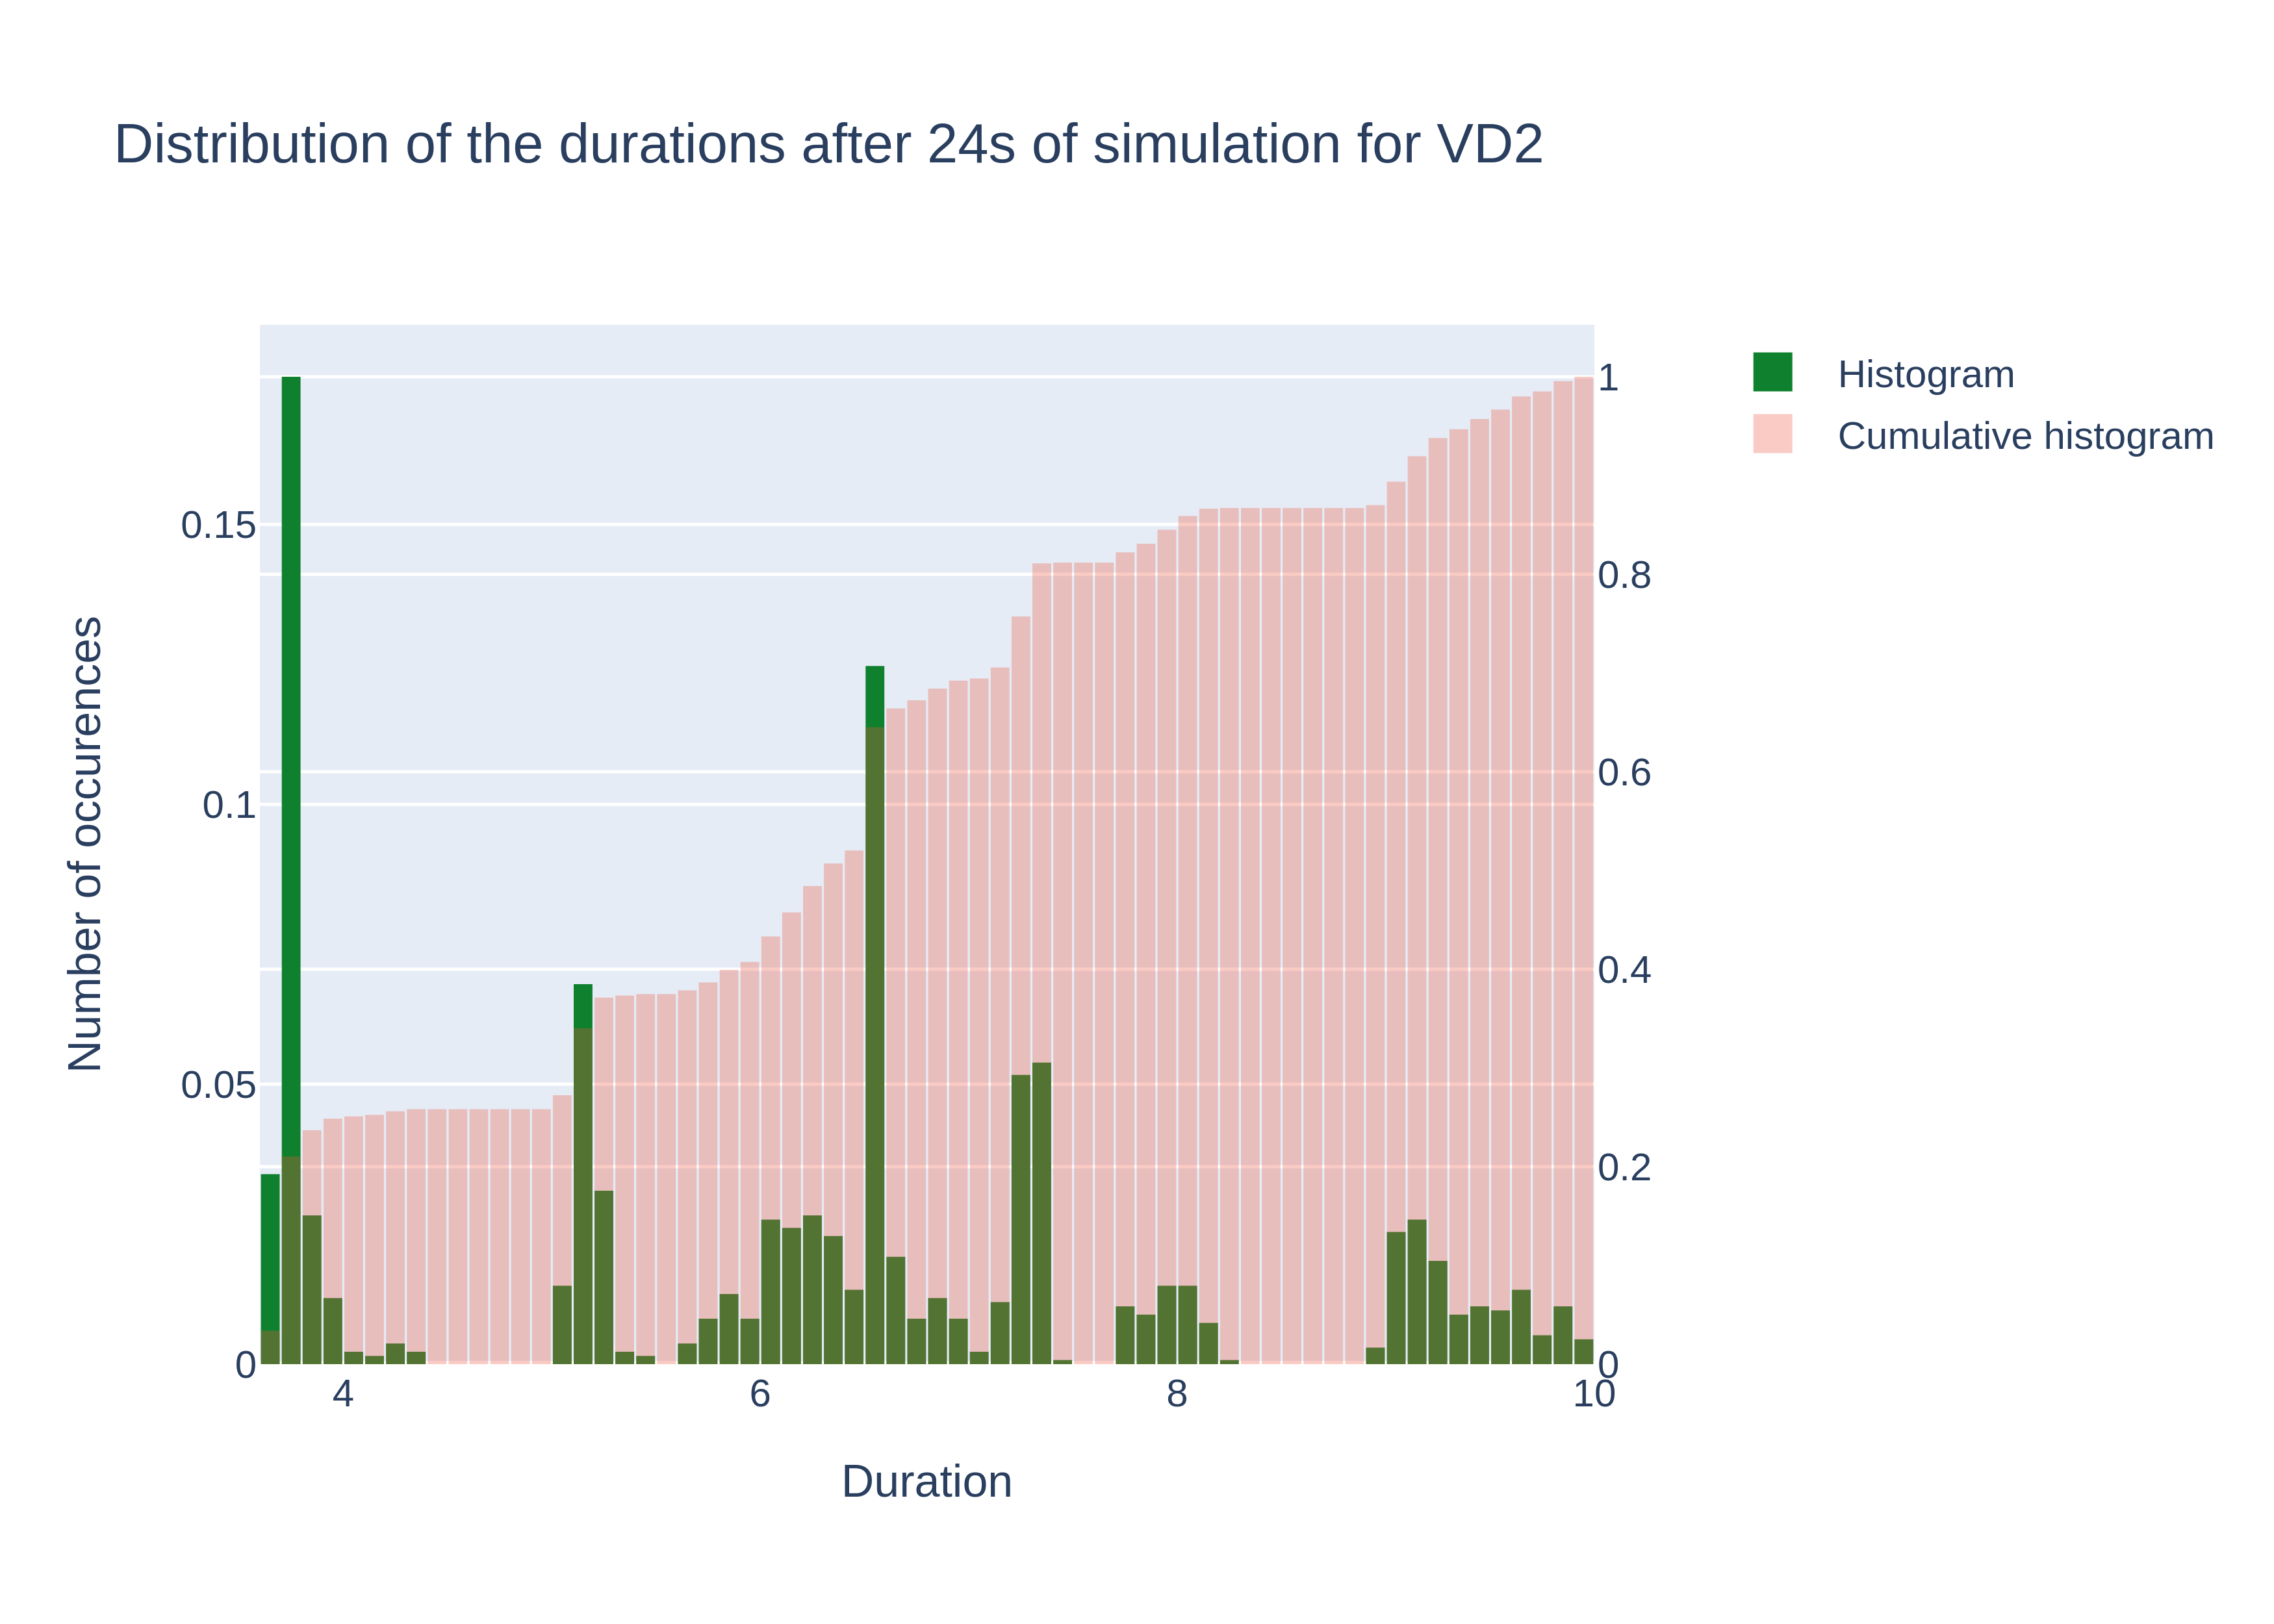
\includegraphics[width=\textwidth]{../fig/data/VD2_24s.png}
        \caption{Simulation time: 24s}
        \vspace{.5cm}
    \end{subfigure}
    \begin{subfigure}{.495\textwidth}
        \centering
        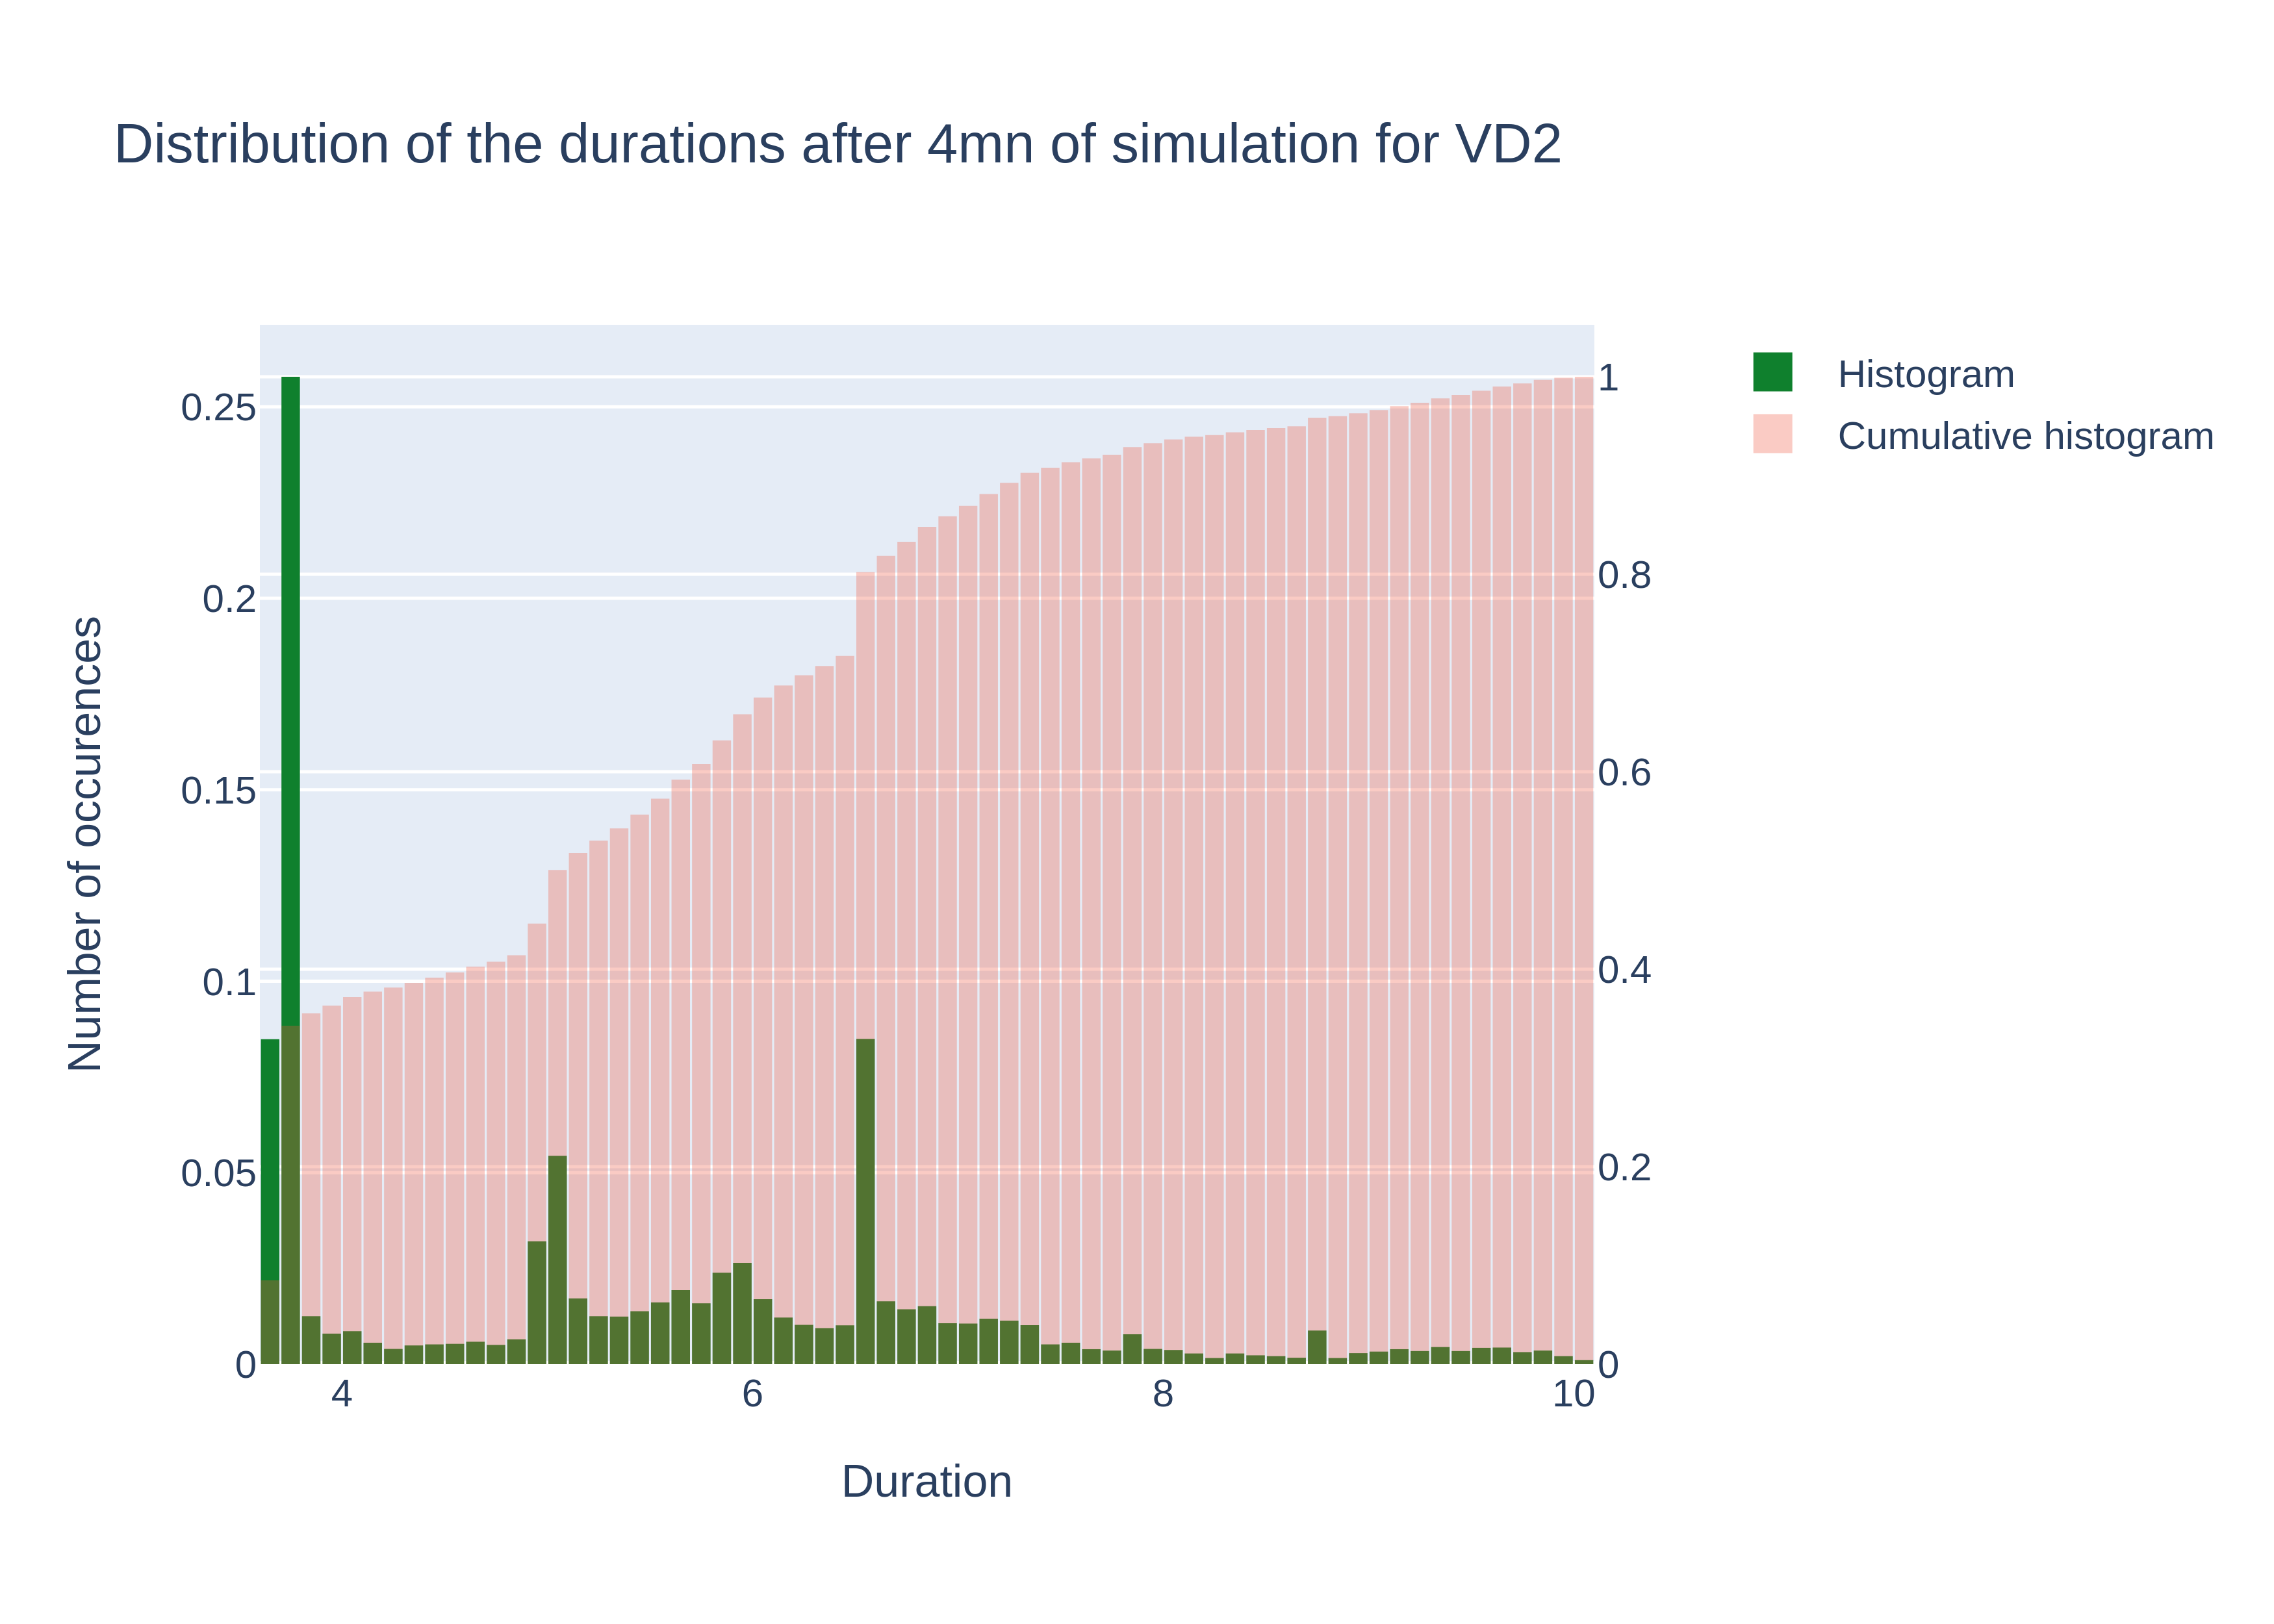
\includegraphics[width=\textwidth]{../fig/data/VD2_4mn.png}
        \caption{Simulation time: 4min}
        \vspace{.5cm}
    \end{subfigure}
    \begin{subfigure}{.495\textwidth}
        \centering
        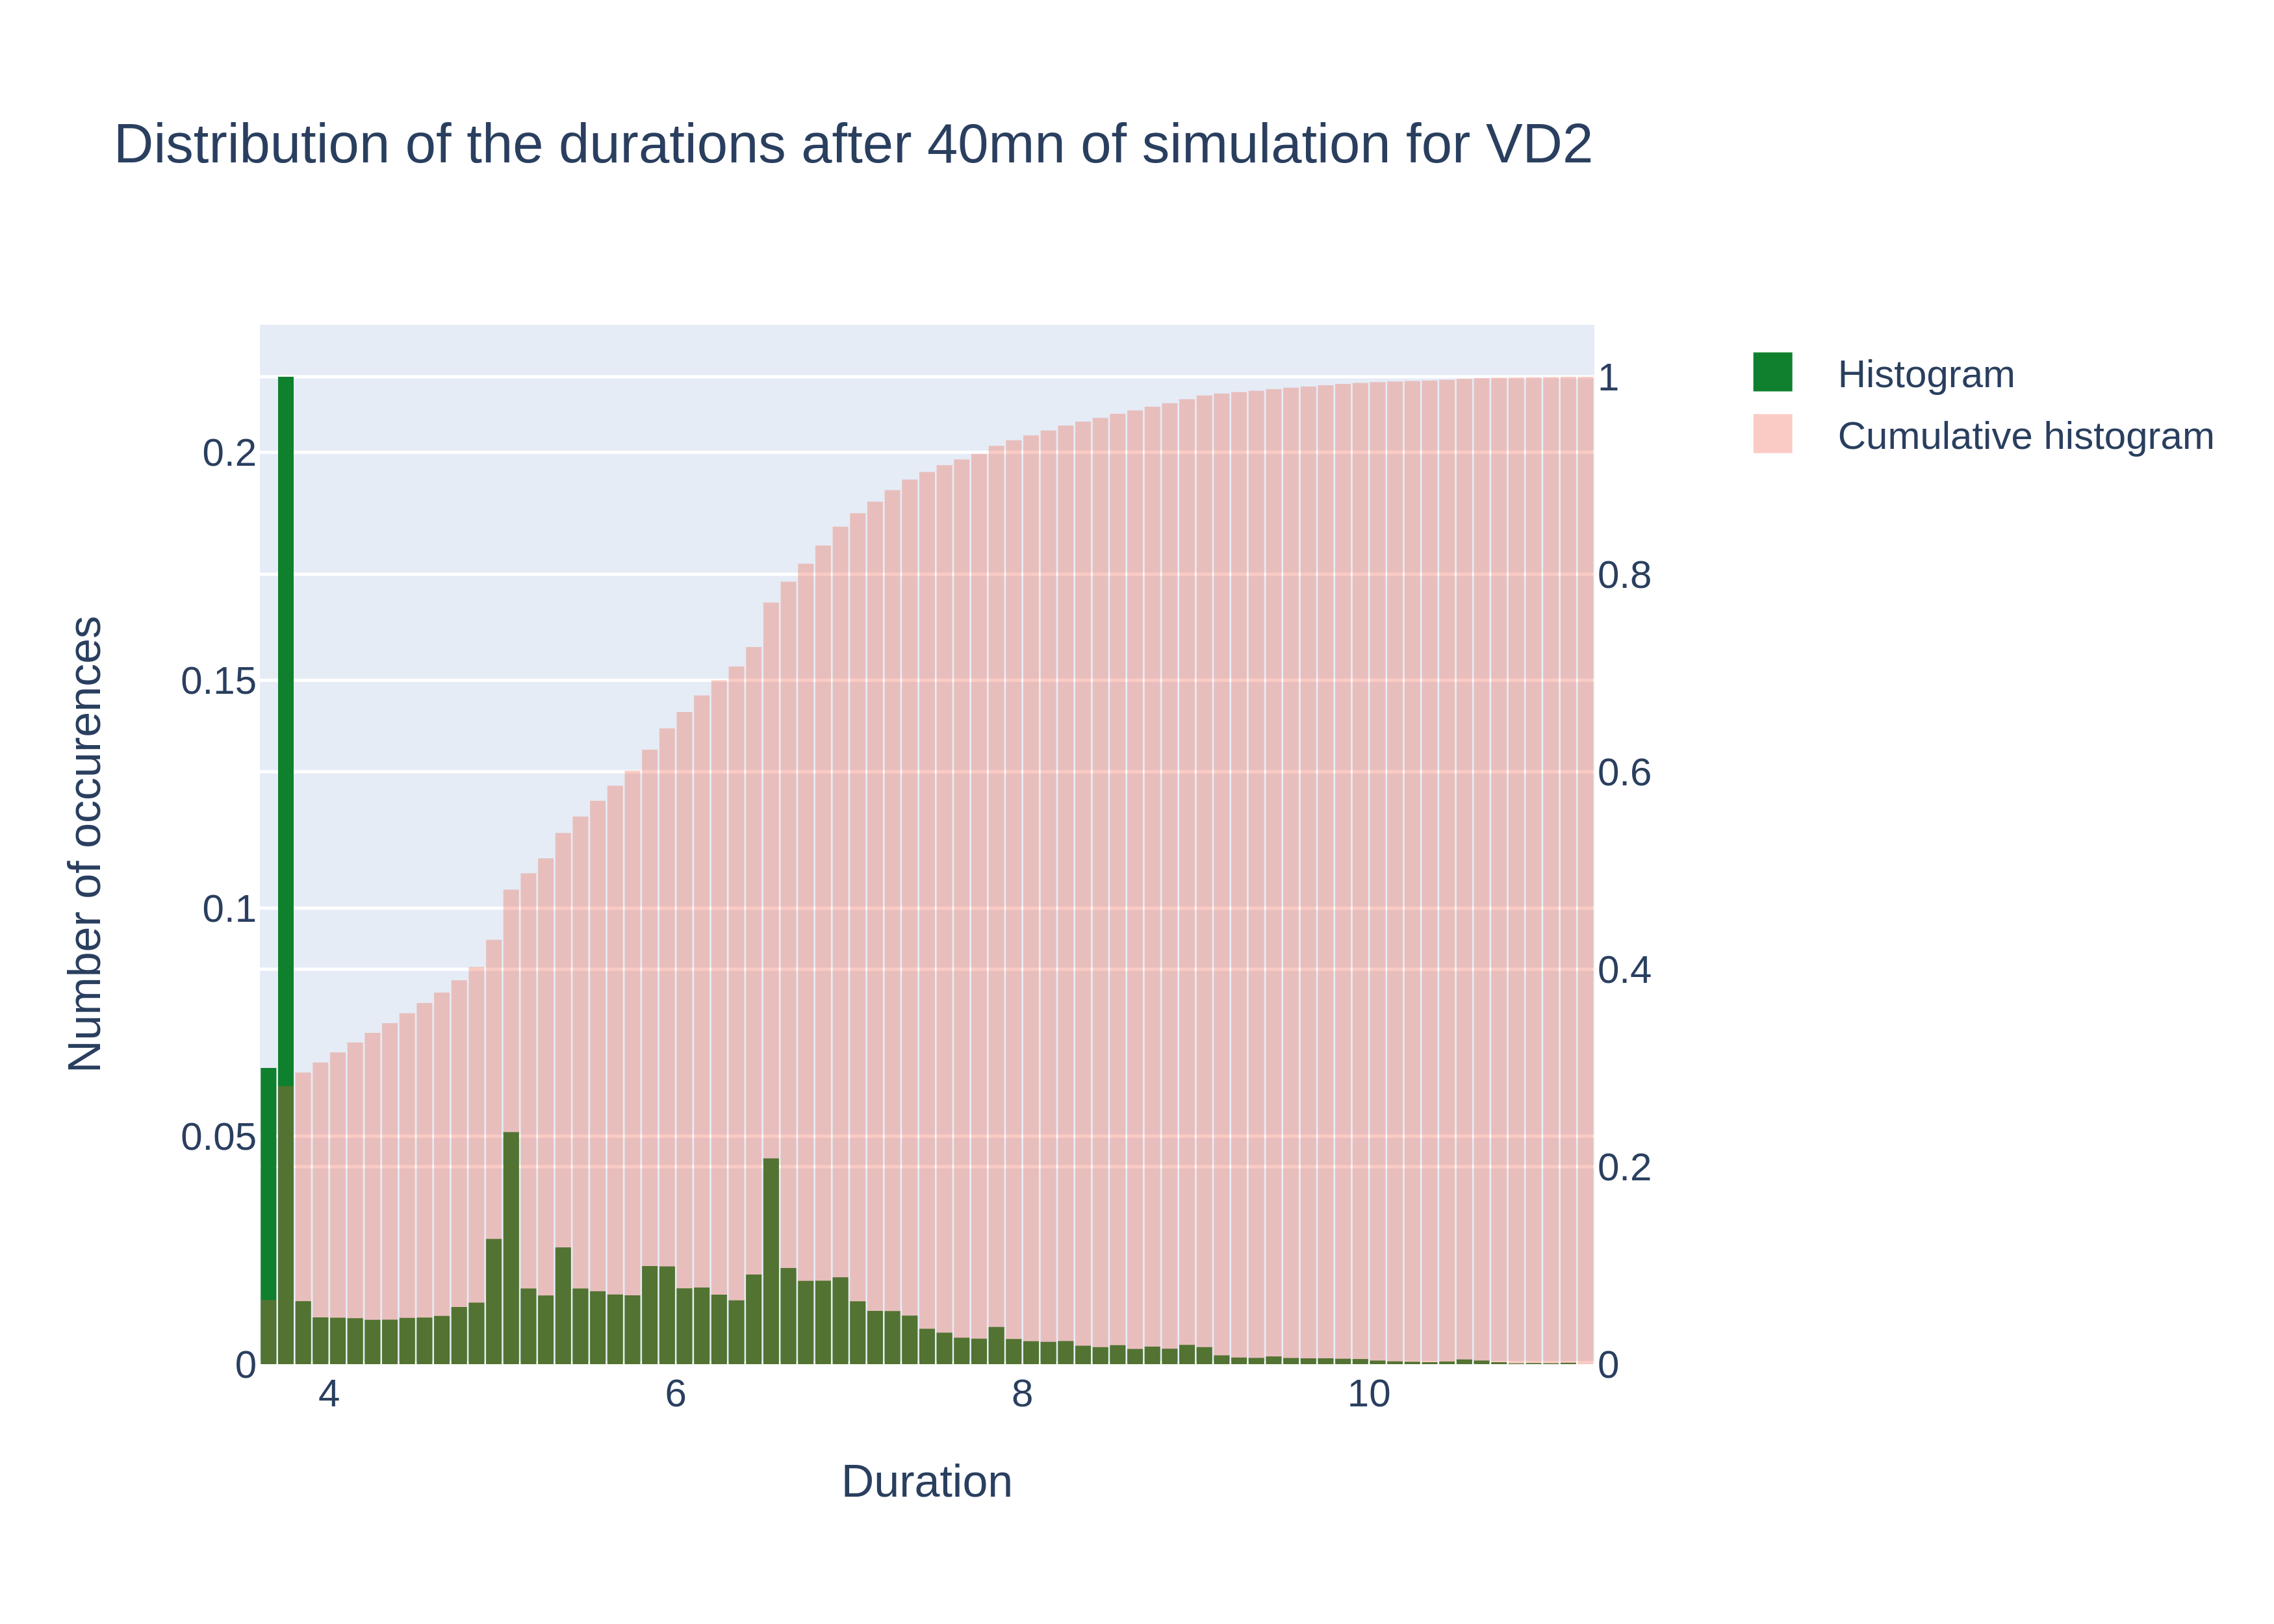
\includegraphics[width=\textwidth]{../fig/data/VD2_40mn.png}
        \caption{Simulation time: 40min}
    \end{subfigure}
    \begin{subfigure}{.495\textwidth}
        \centering
        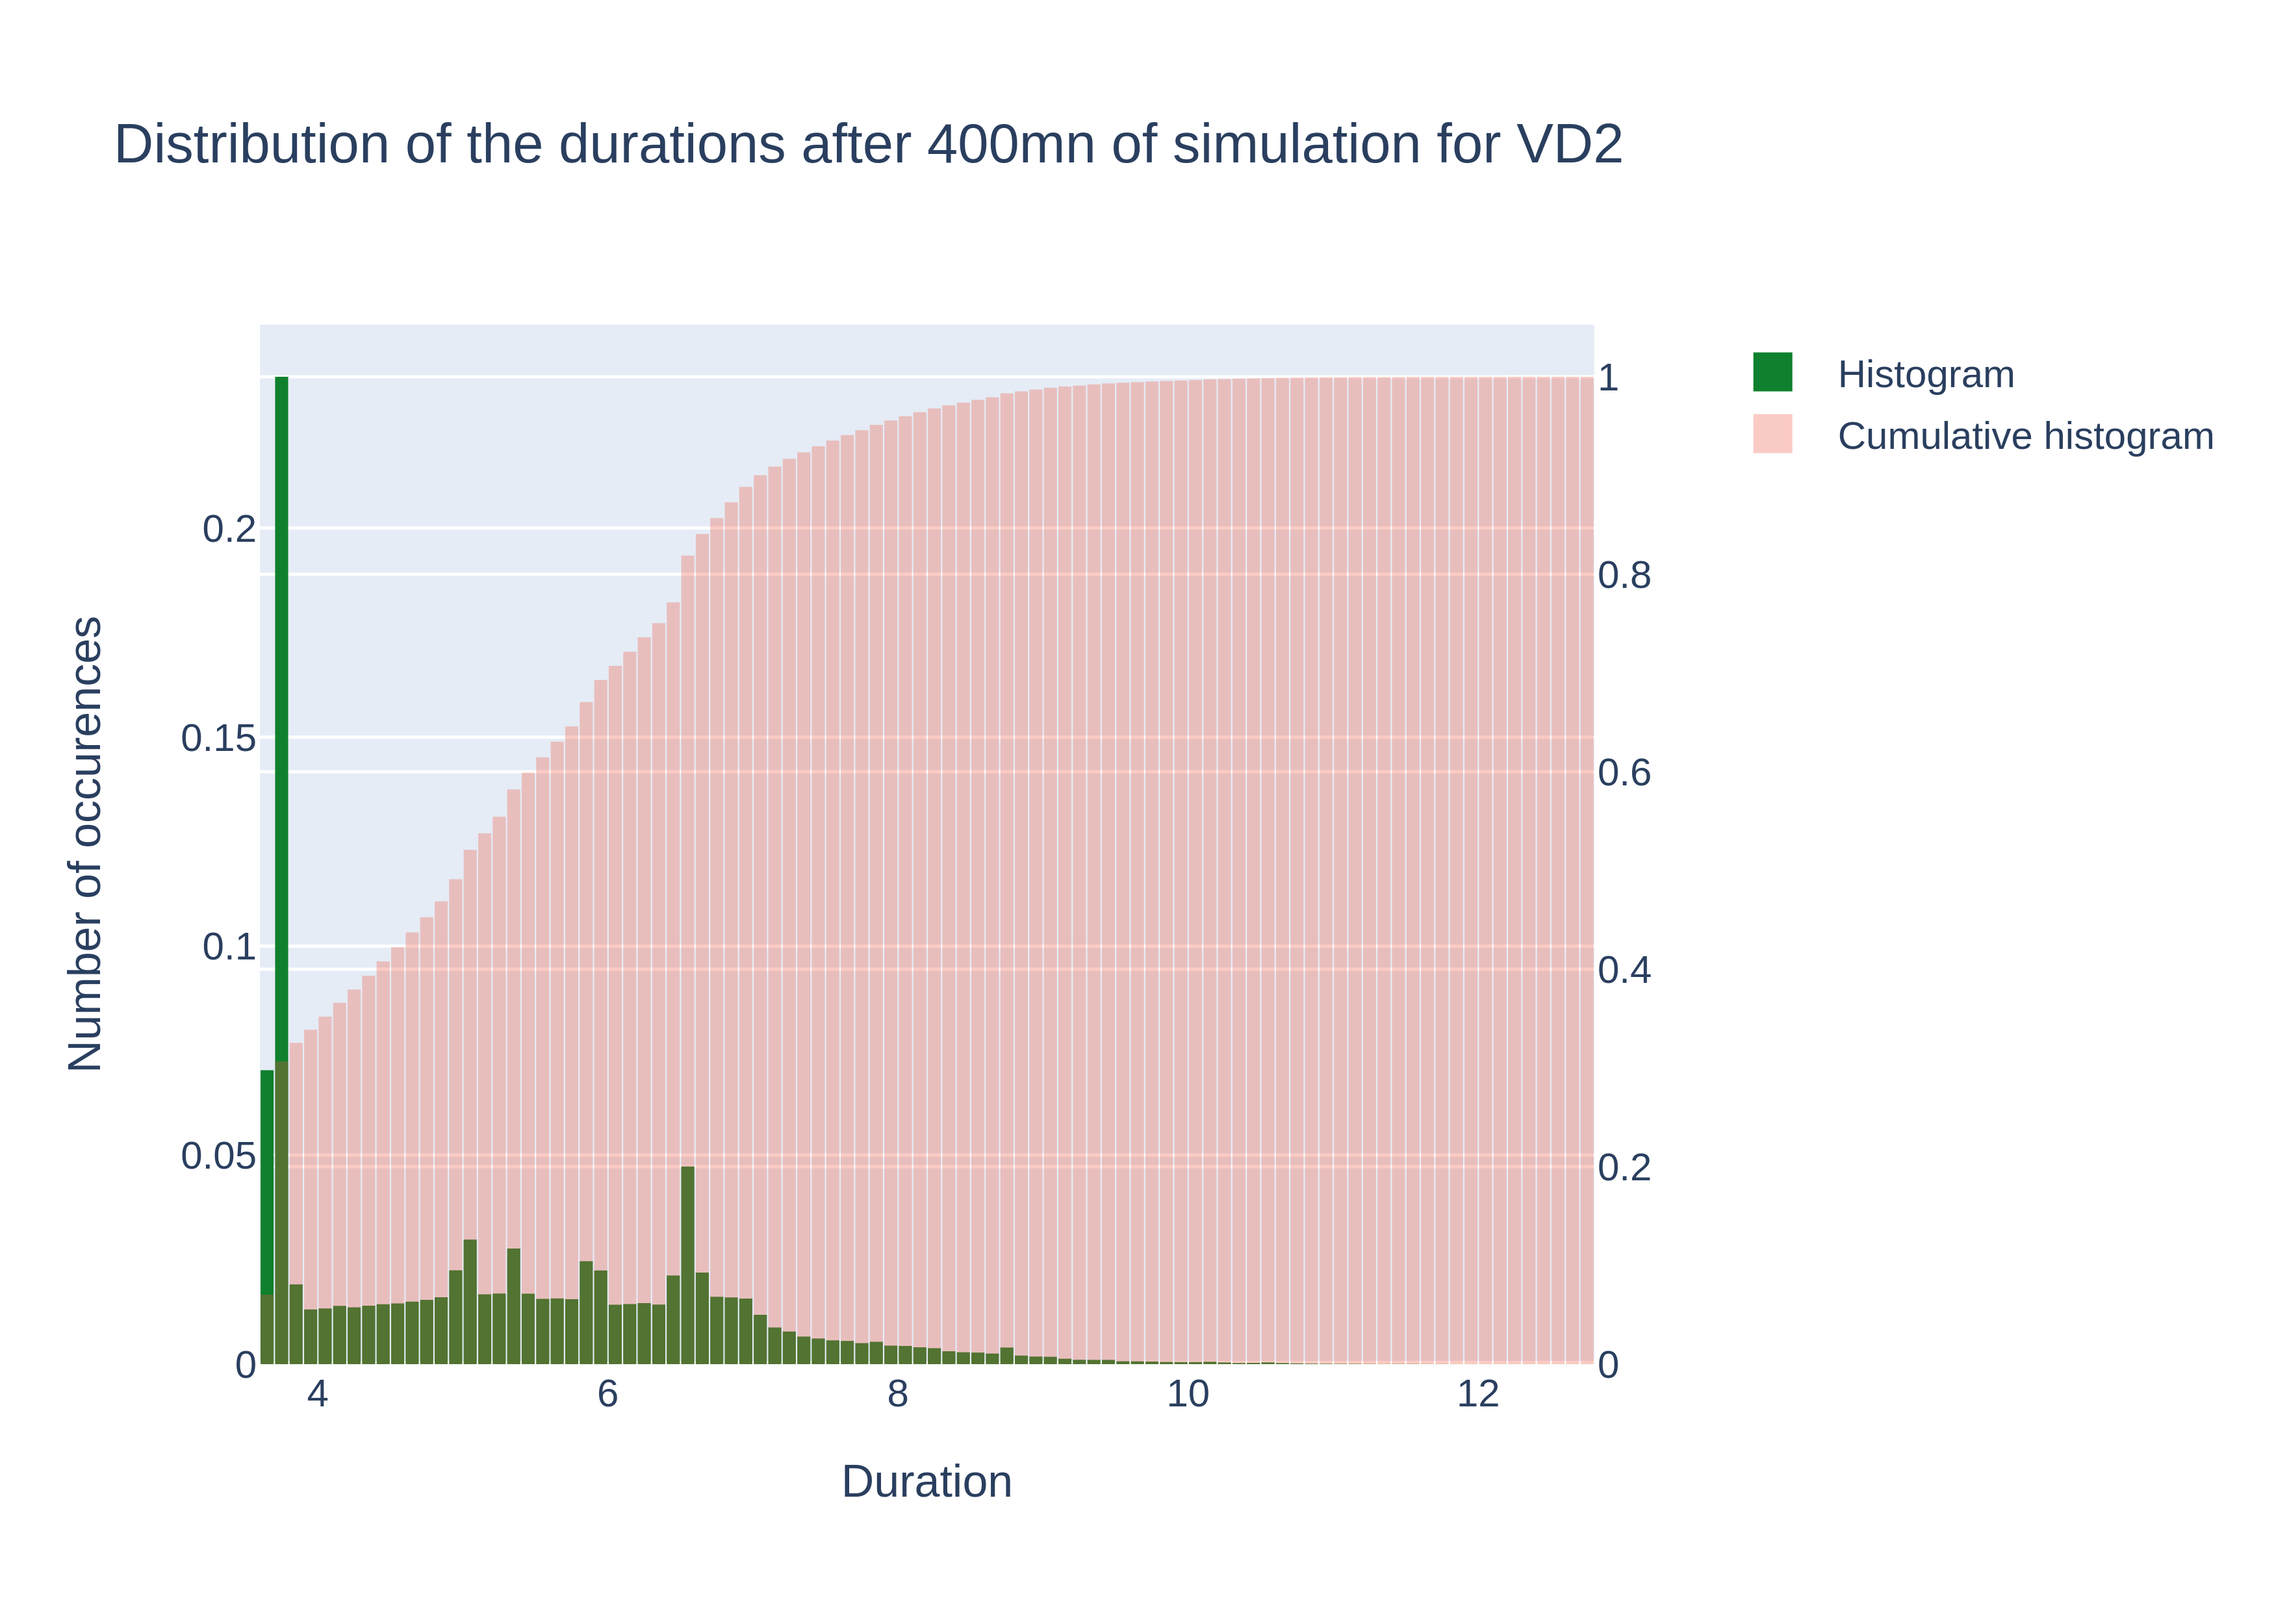
\includegraphics[width=\textwidth]{../fig/data/VD2_400mn.png}
        \caption{Simulation time: 400min}
    \end{subfigure}
    \caption{VD2 data after multiple simulation times}
\end{figure}

\subsubsection{Quantile 3}
\begin{figure}[H]
    \centering
    \begin{subfigure}{.495\textwidth}
        \centering
        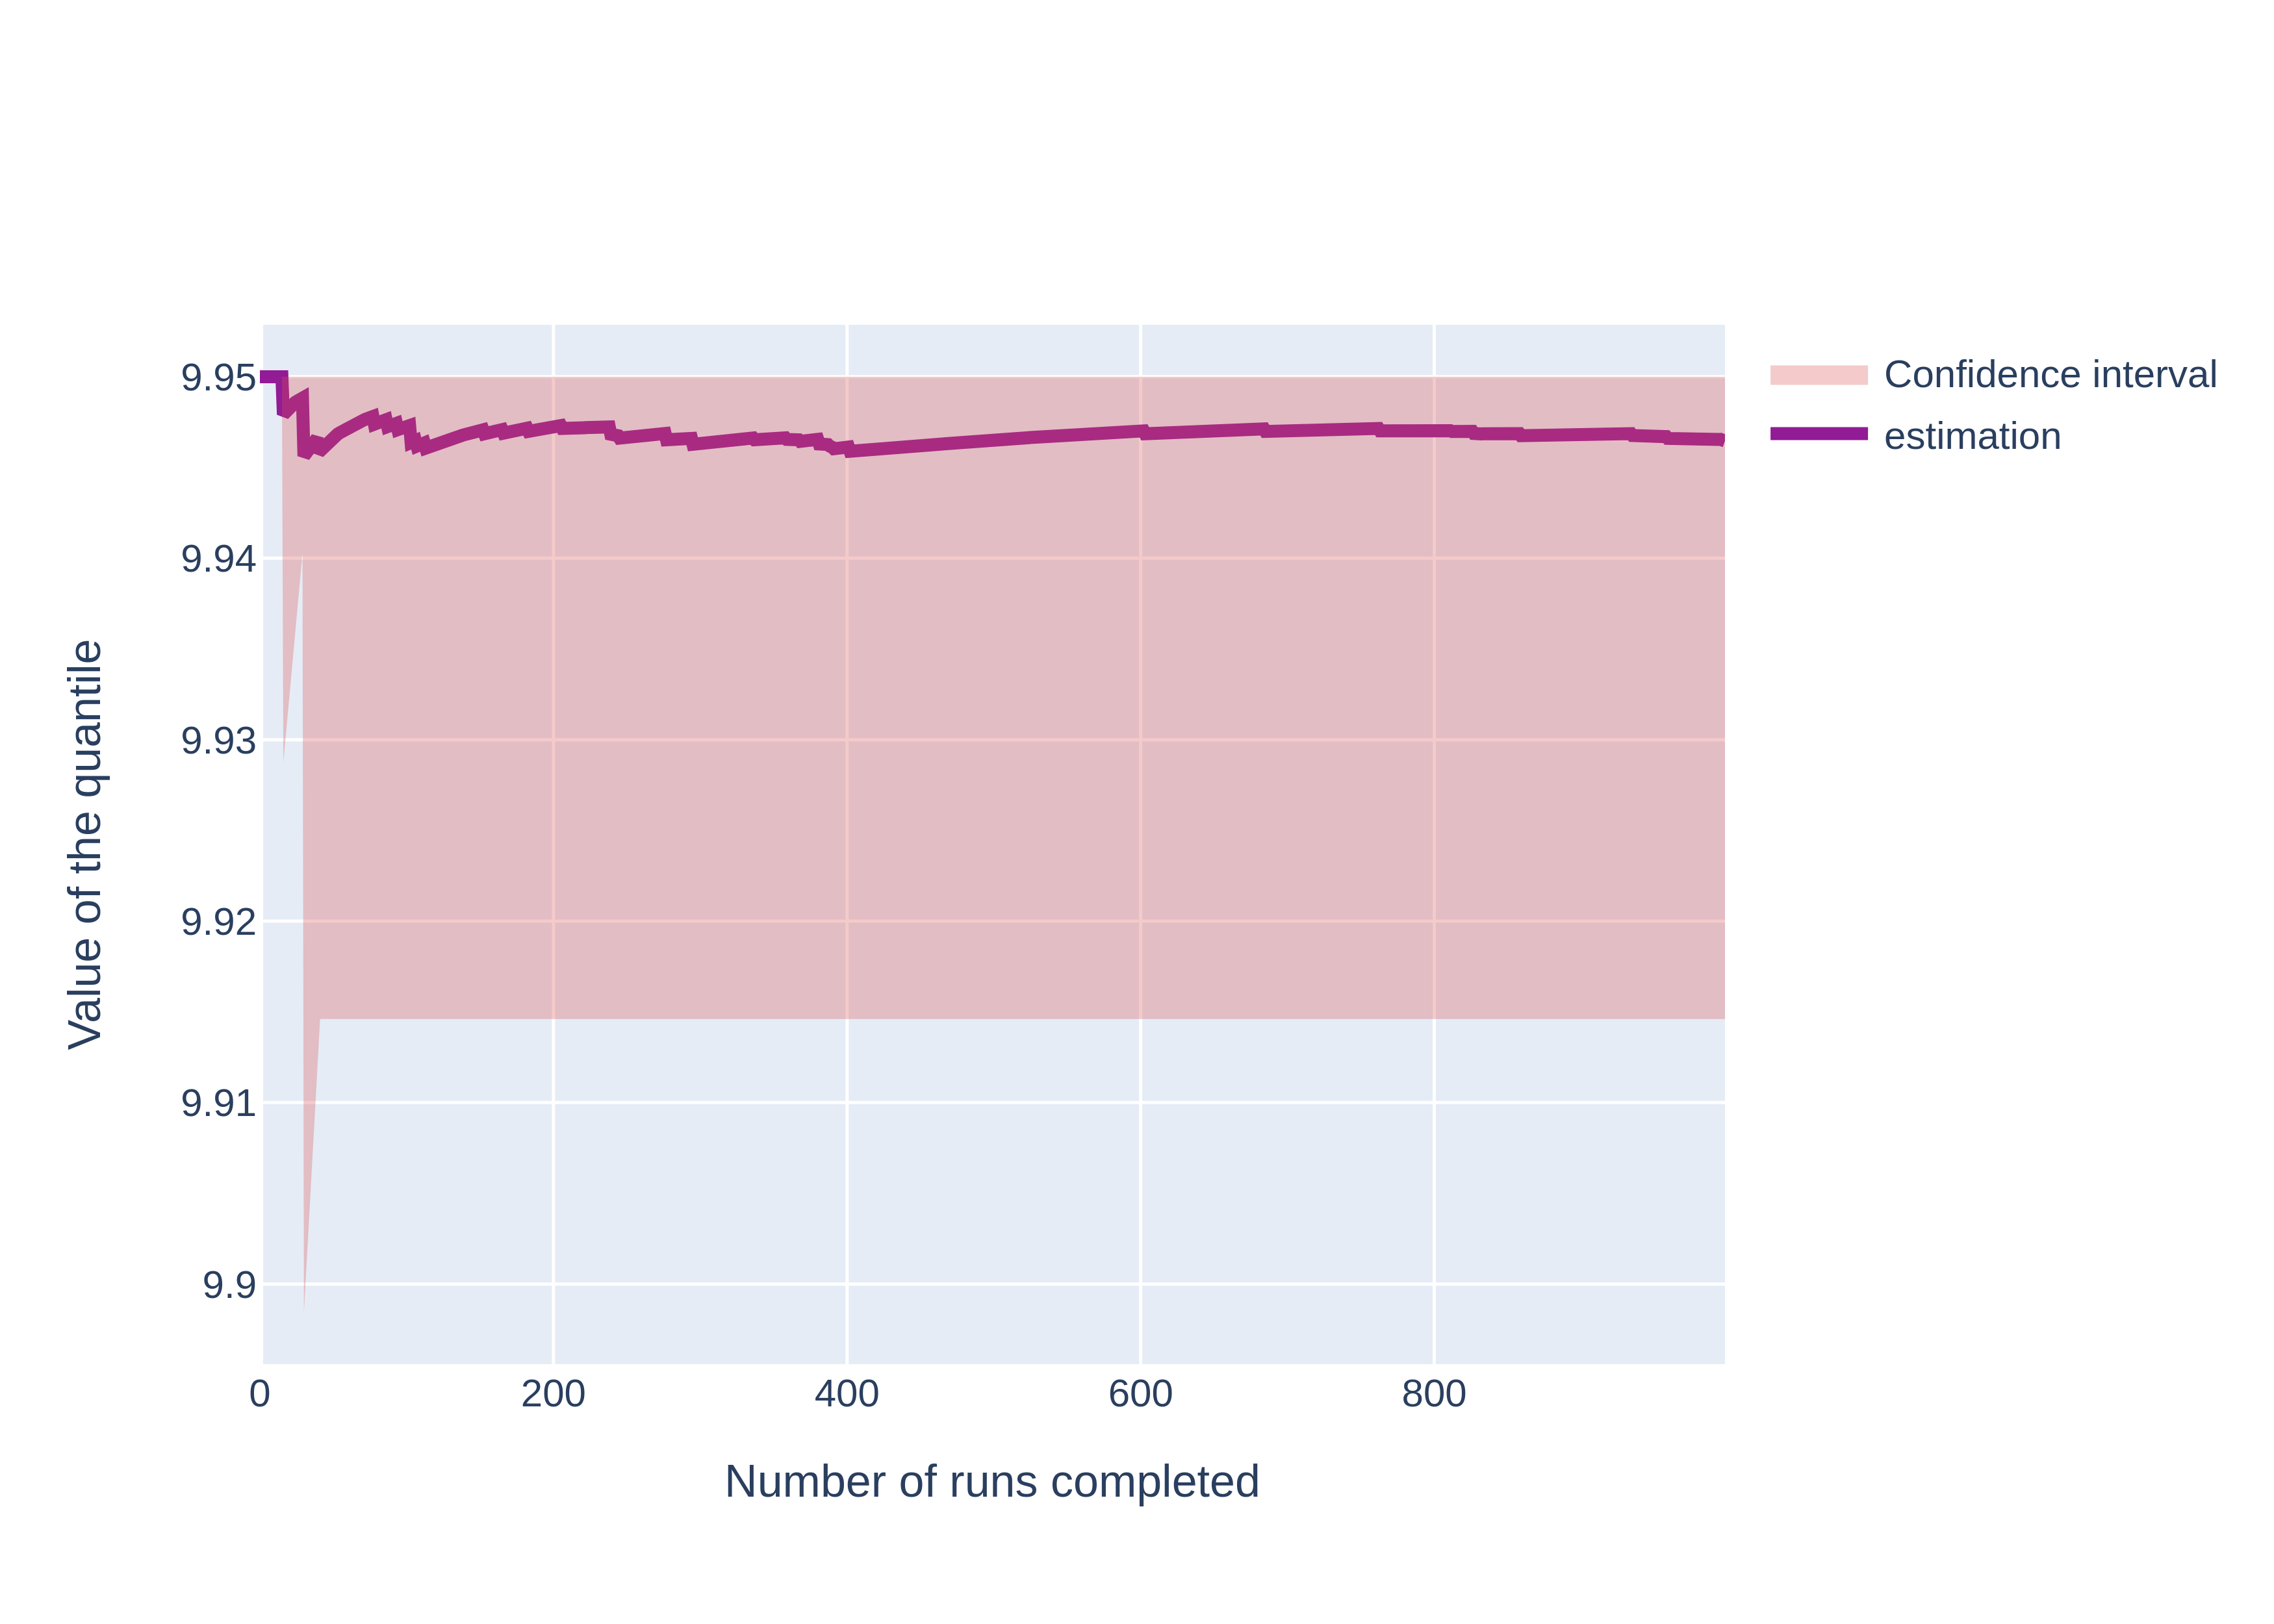
\includegraphics[width=\textwidth]{../fig/quantile3/VD2_24s.png}
        \caption{Simulation time: 24s}
        \vspace{.5cm}
    \end{subfigure}
    \begin{subfigure}{.495\textwidth}
        \centering
        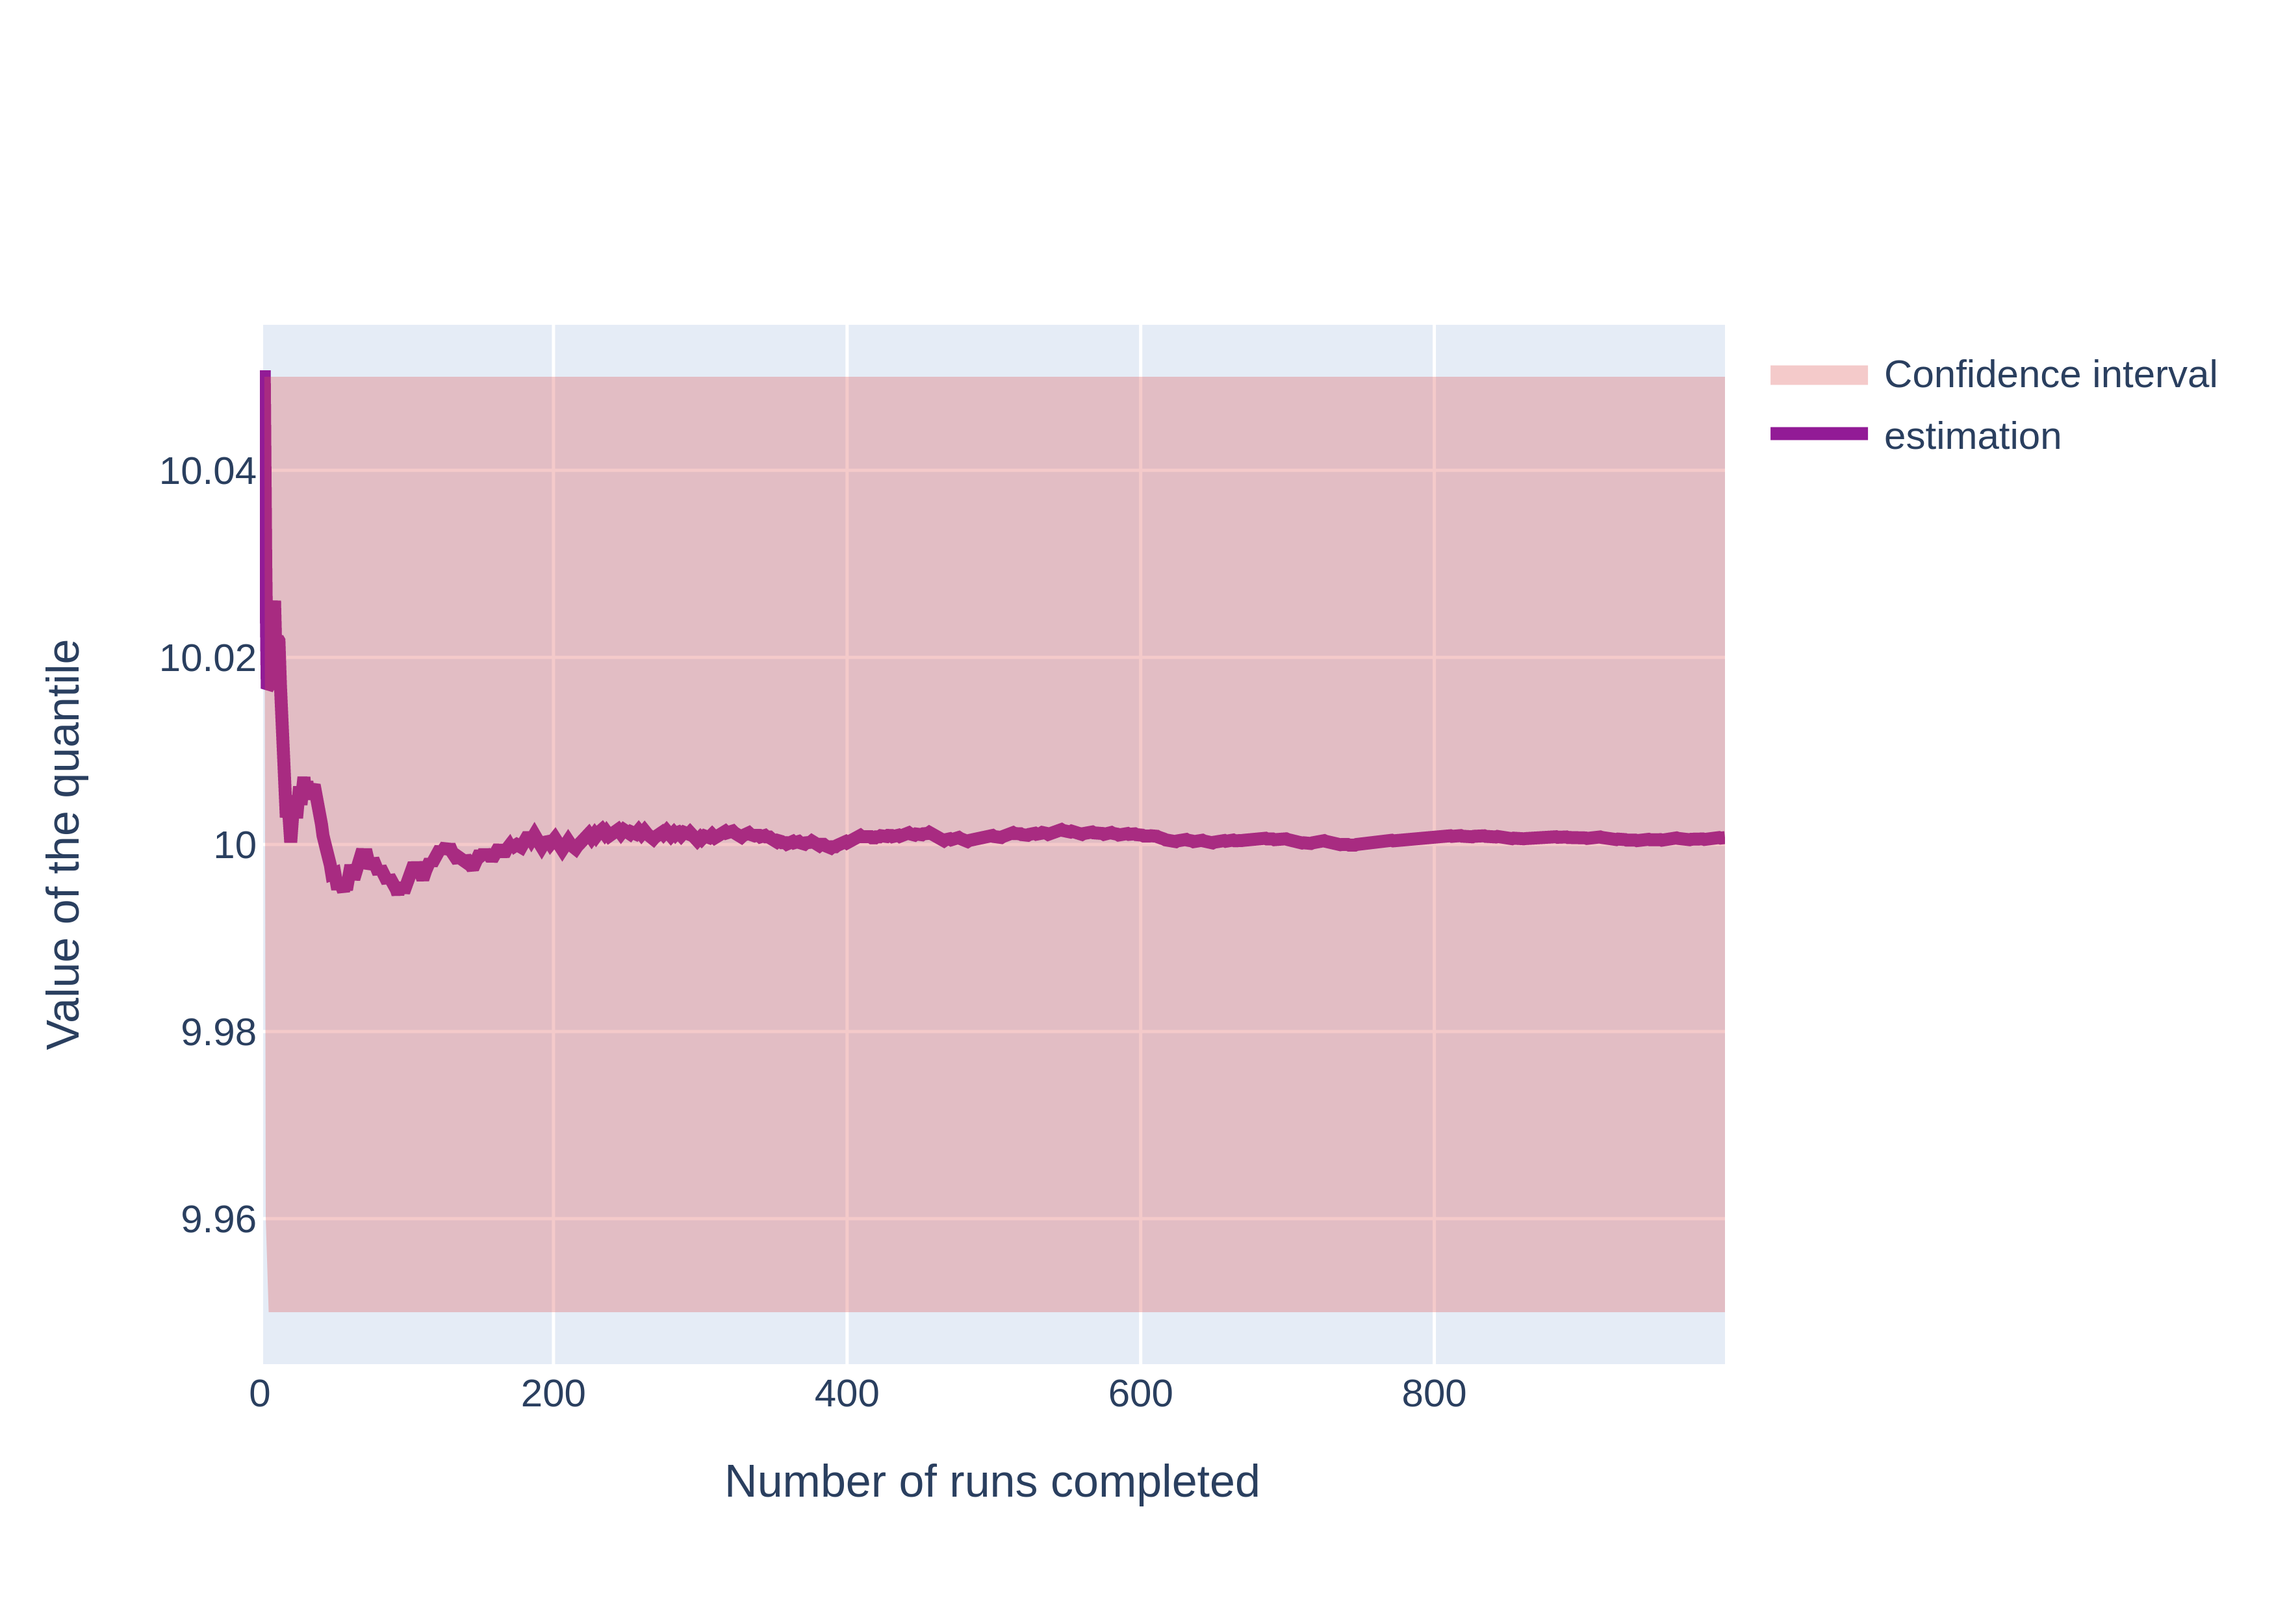
\includegraphics[width=\textwidth]{../fig/quantile3/VD2_4mn.png}
        \caption{Simulation time: 4min}
        \vspace{.5cm}
    \end{subfigure}
    \begin{subfigure}{.495\textwidth}
        \centering
        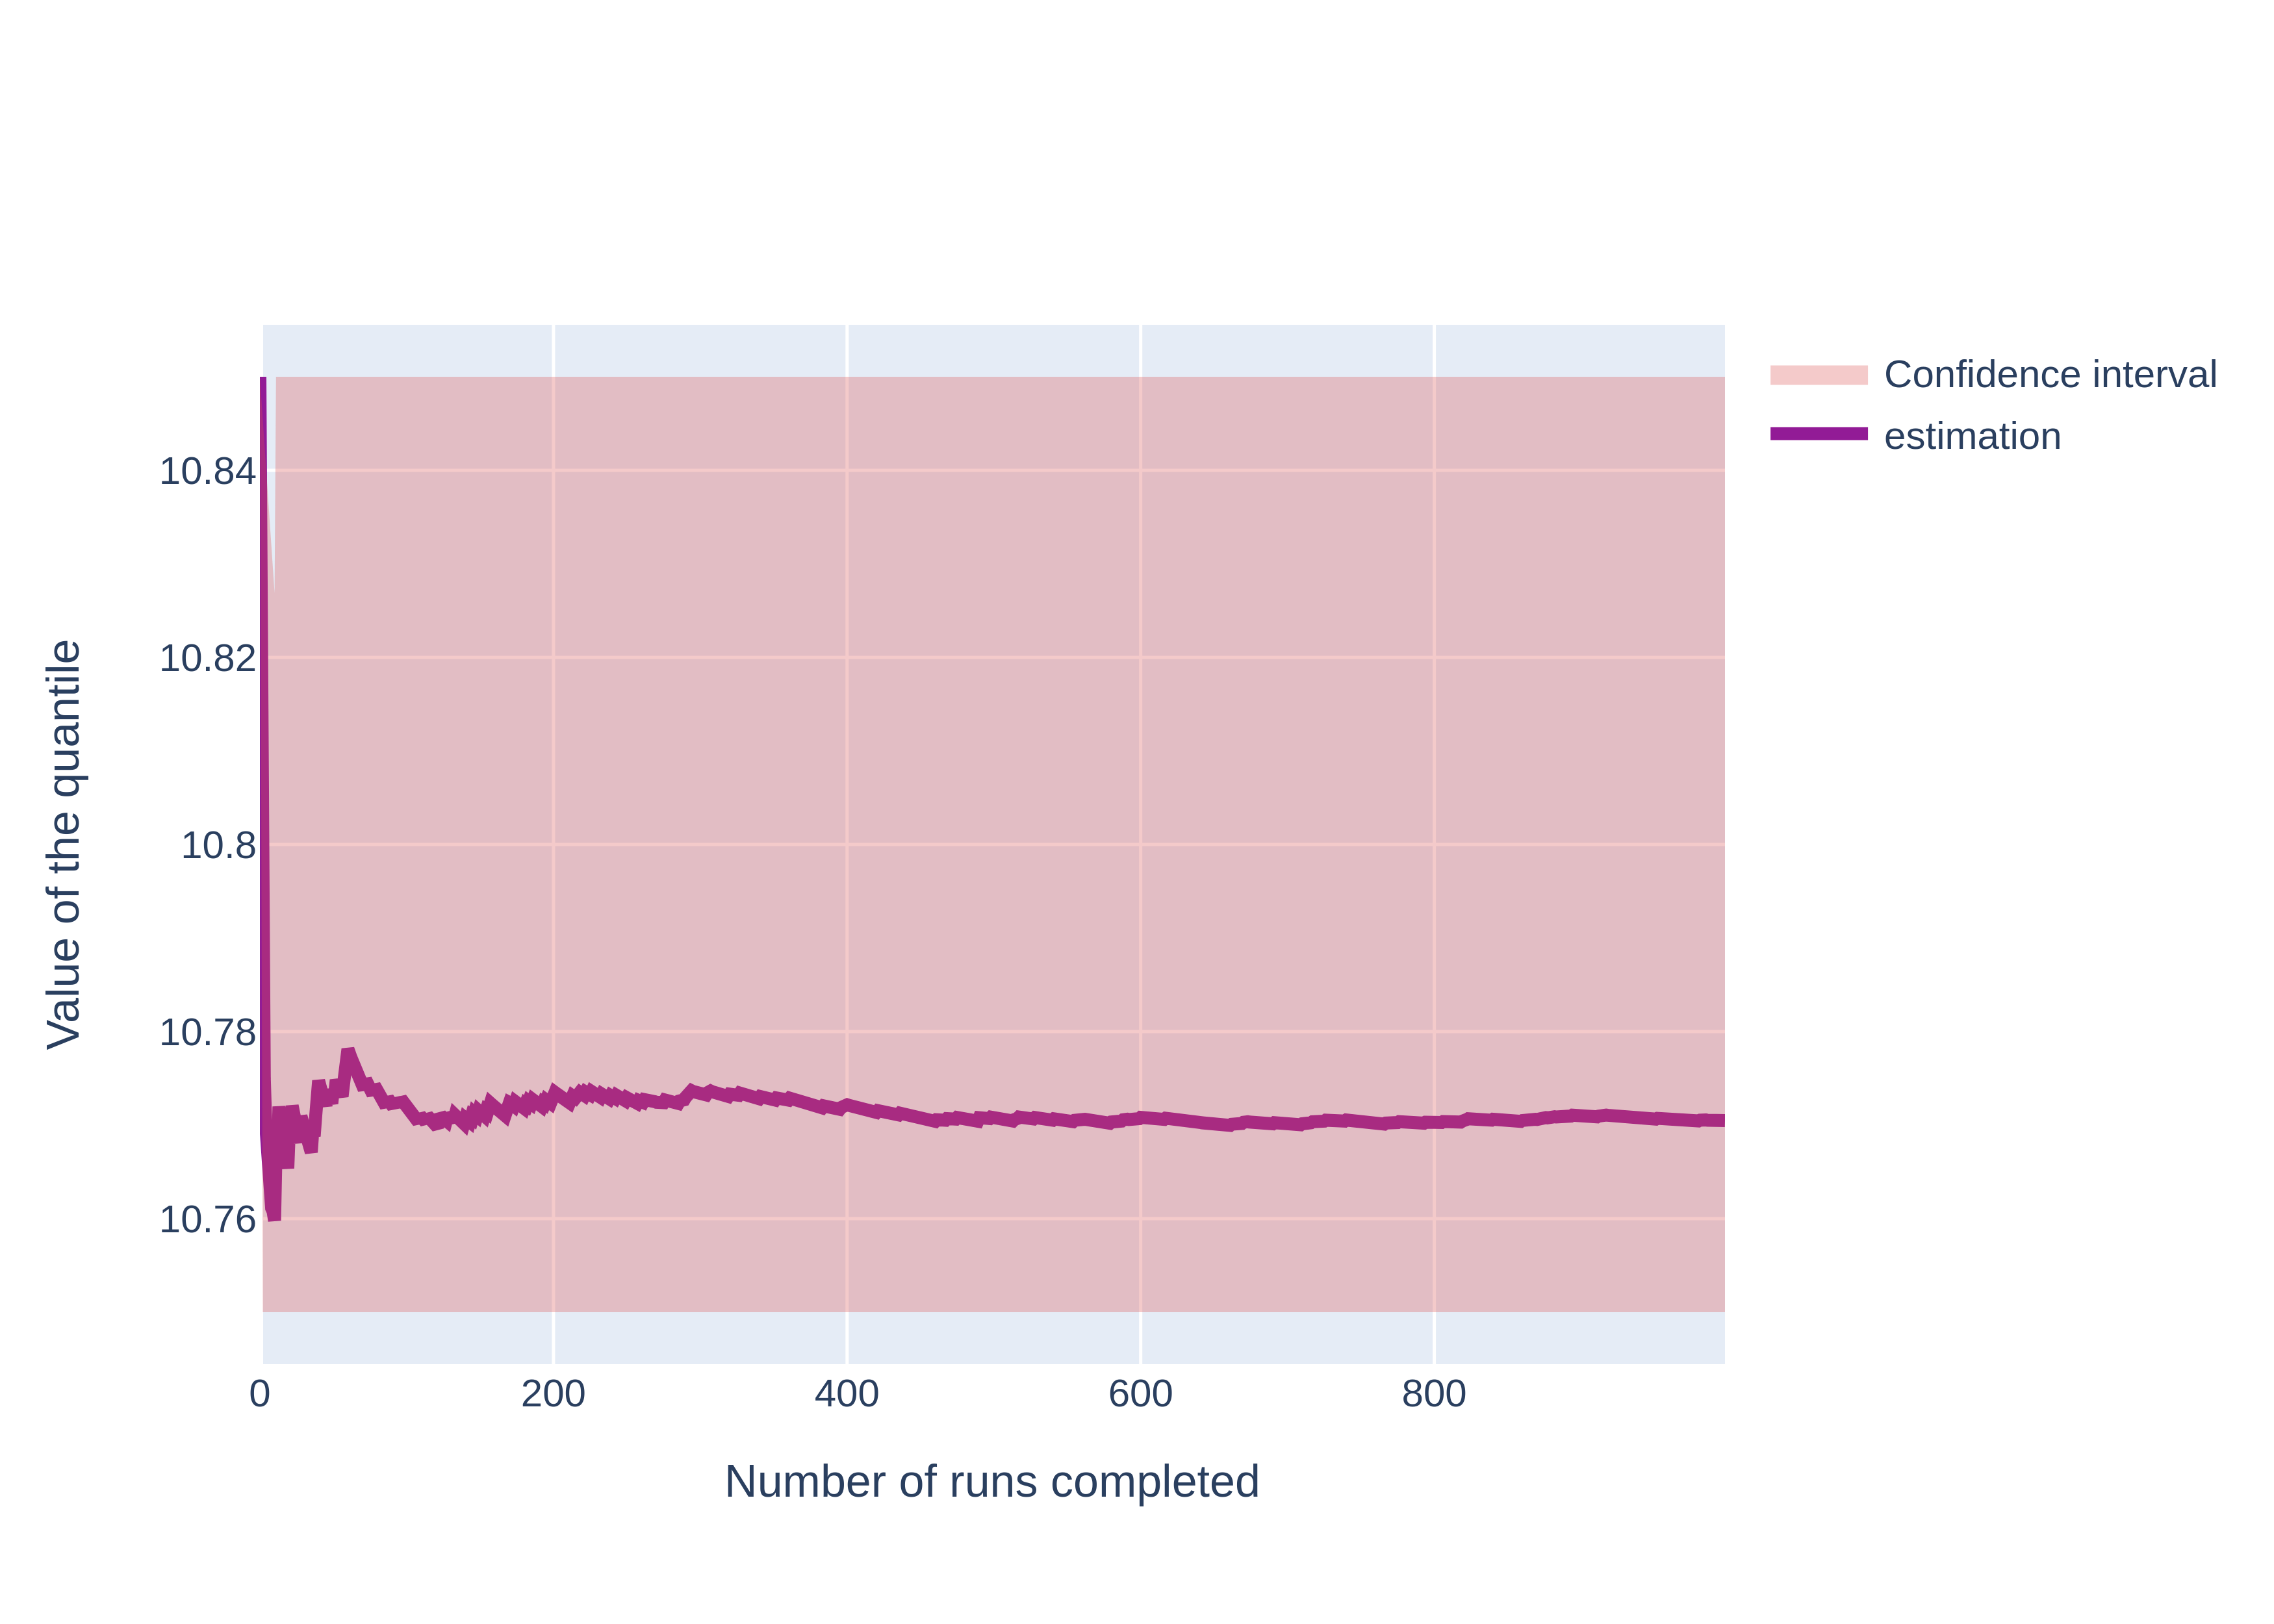
\includegraphics[width=\textwidth]{../fig/quantile3/VD2_40mn.png}
        \caption{Simulation time: 40min}
    \end{subfigure}
    \begin{subfigure}{.495\textwidth}
        \centering
        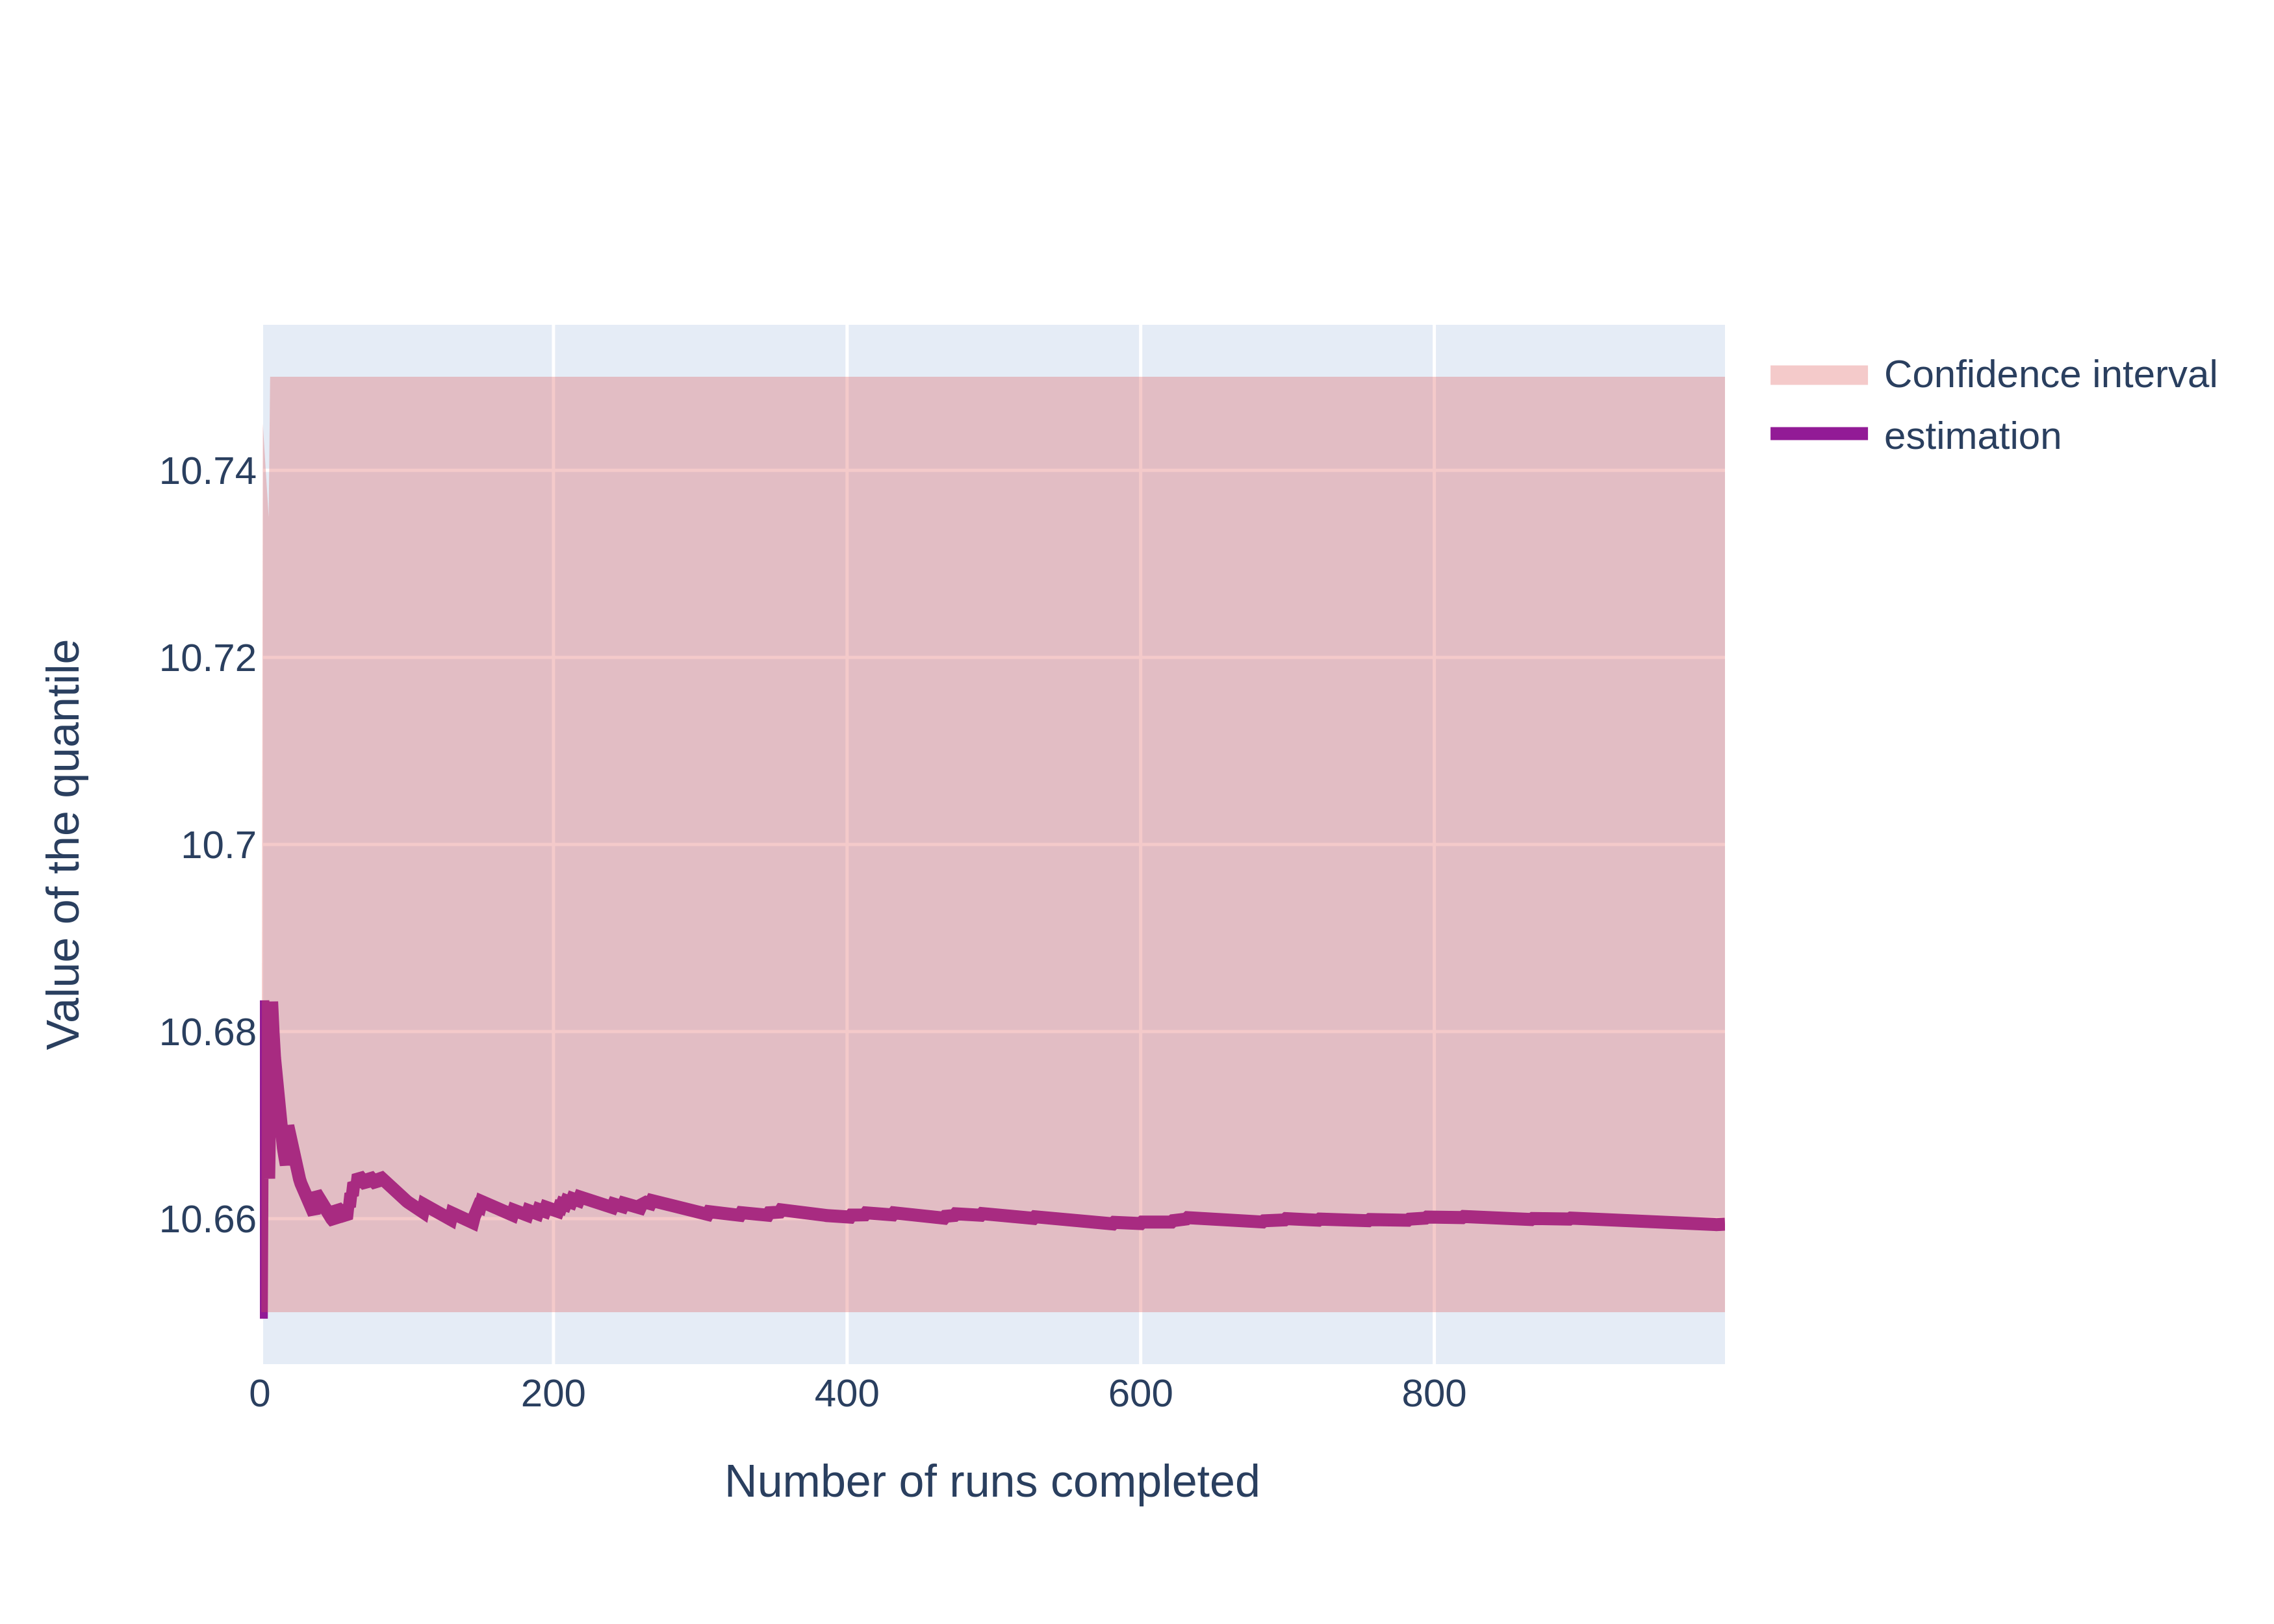
\includegraphics[width=\textwidth]{../fig/quantile3/VD2_400mn.png}
        \caption{Simulation time: 400min}
    \end{subfigure}
    \caption{VD2 $q_3$ after multiple simulation times}
\end{figure}

\subsubsection{Quantile 4}
\begin{figure}[H]
    \centering
    \begin{subfigure}{.495\textwidth}
        \centering
        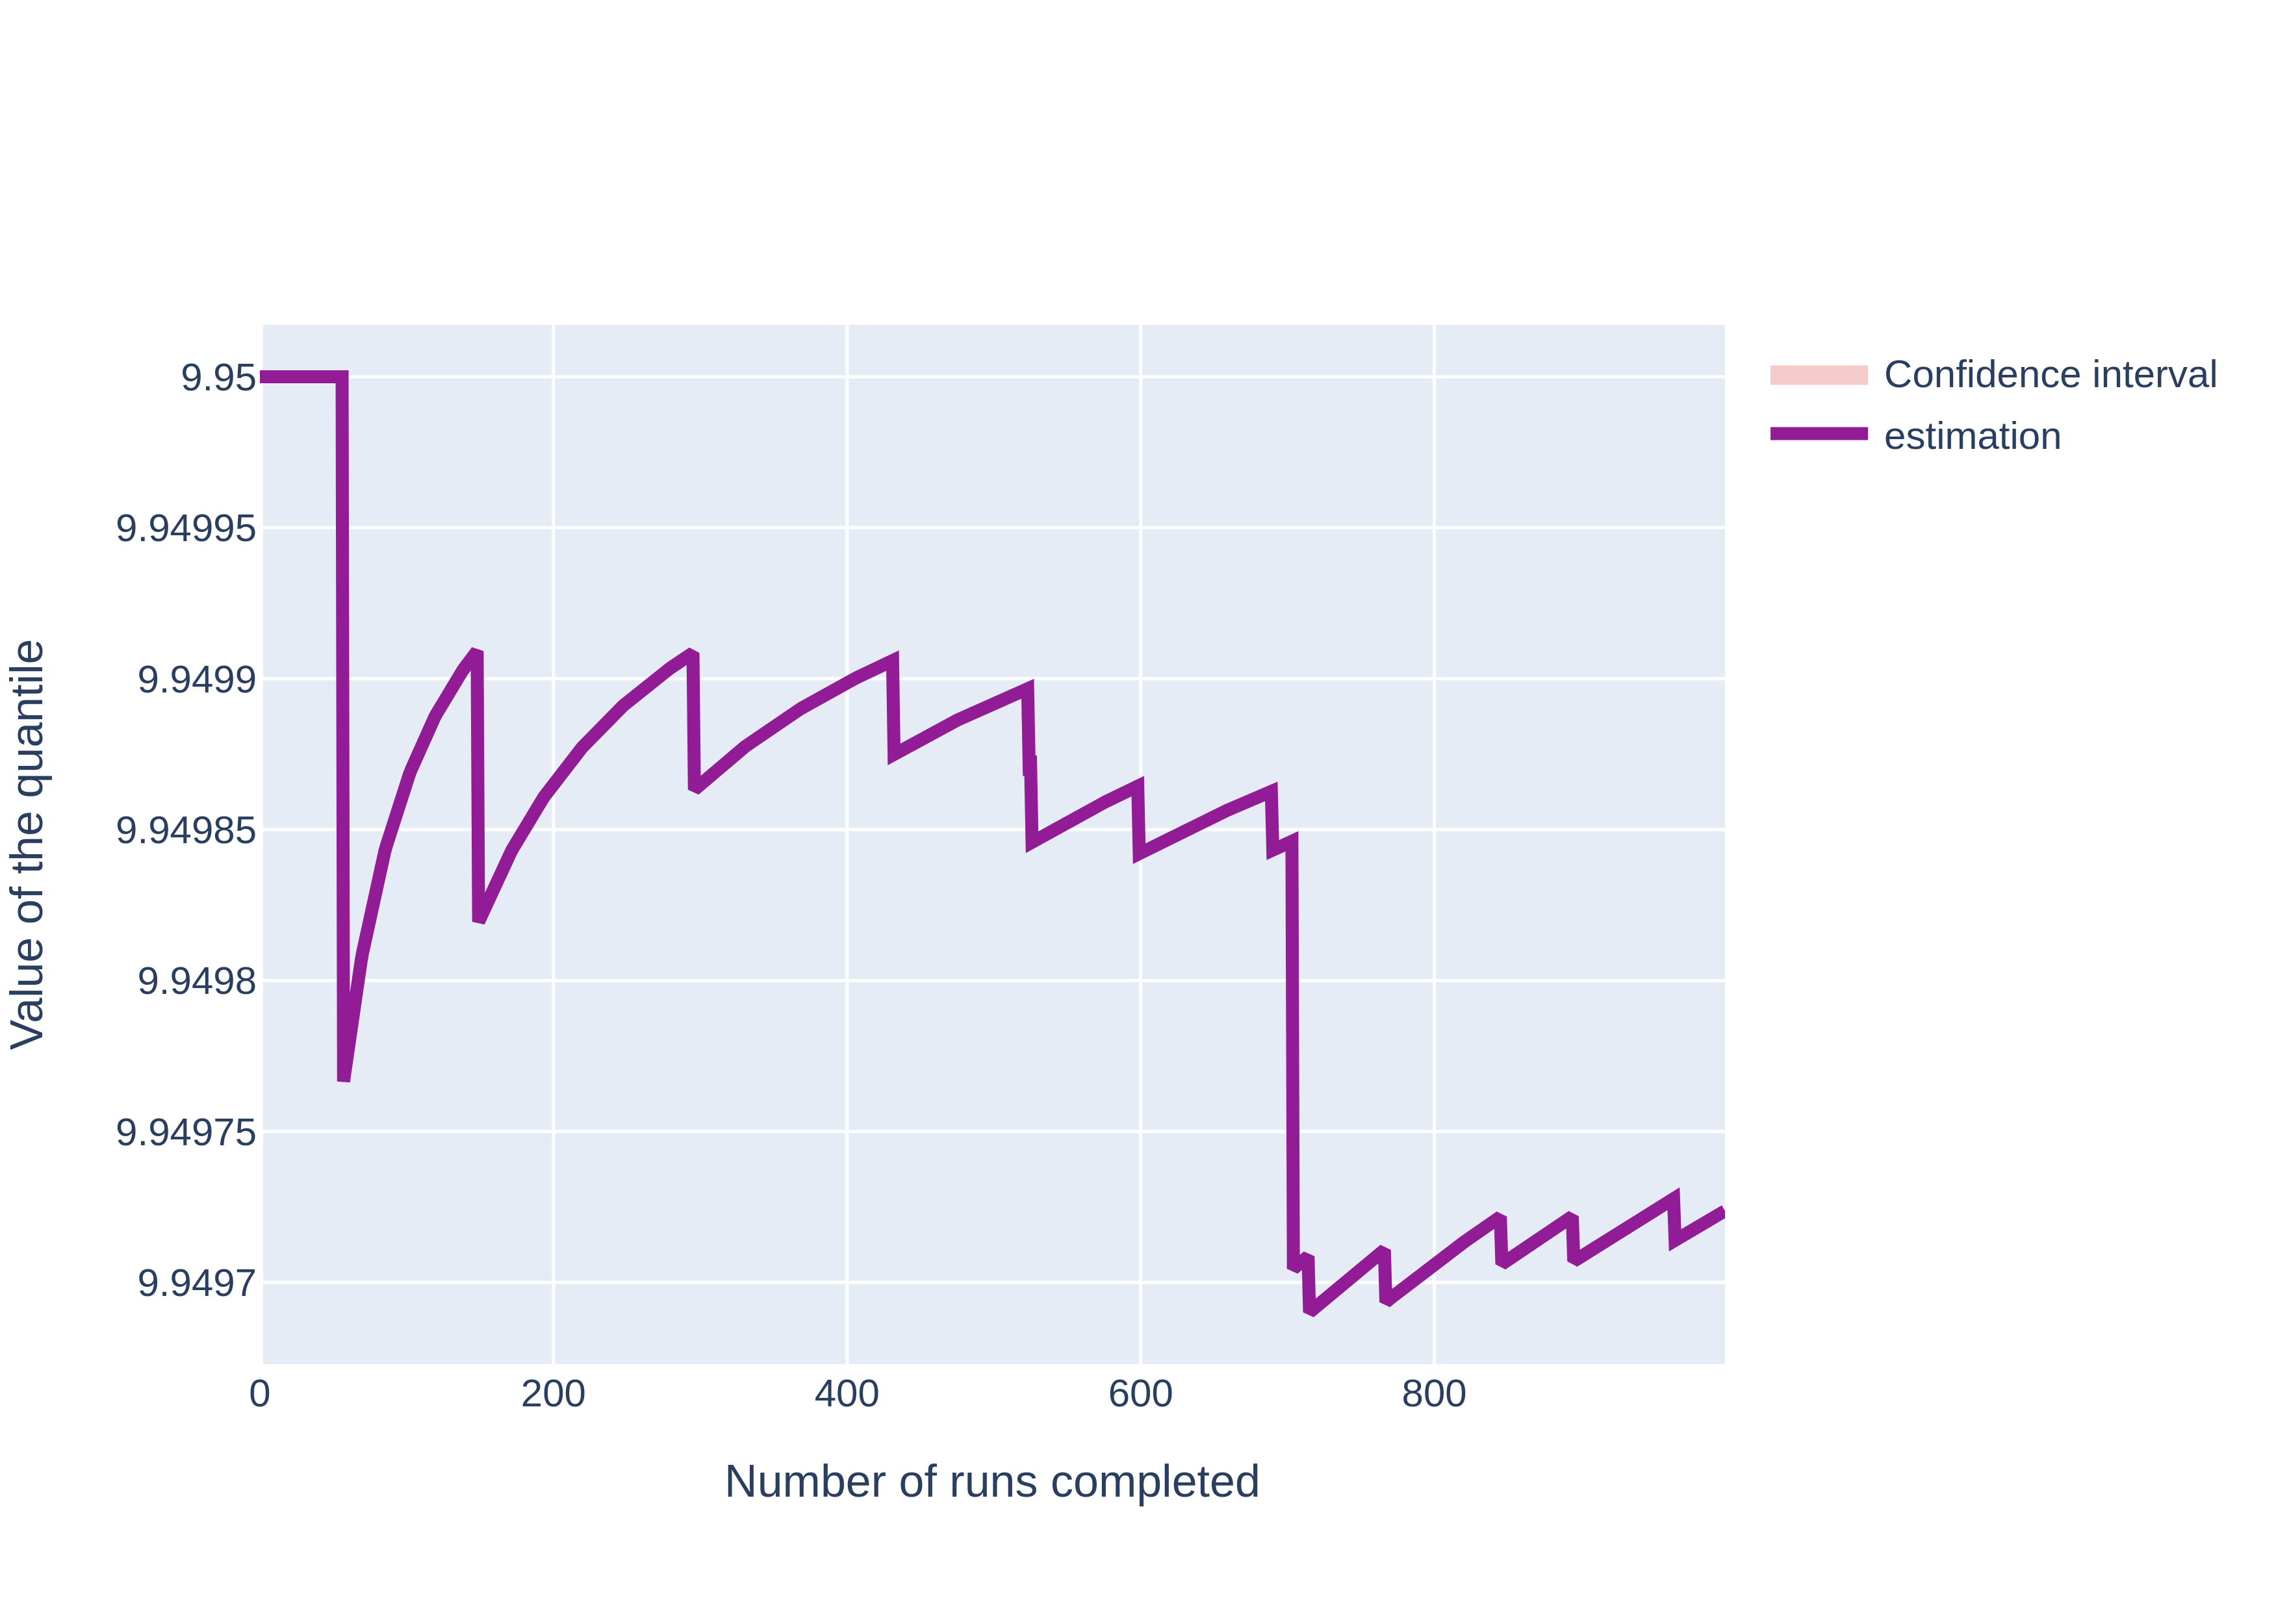
\includegraphics[width=\textwidth]{../fig/quantile4/VD2_24s.png}
        \caption{Simulation time: 24s}
        \vspace{.5cm}
    \end{subfigure}
    \begin{subfigure}{.495\textwidth}
        \centering
        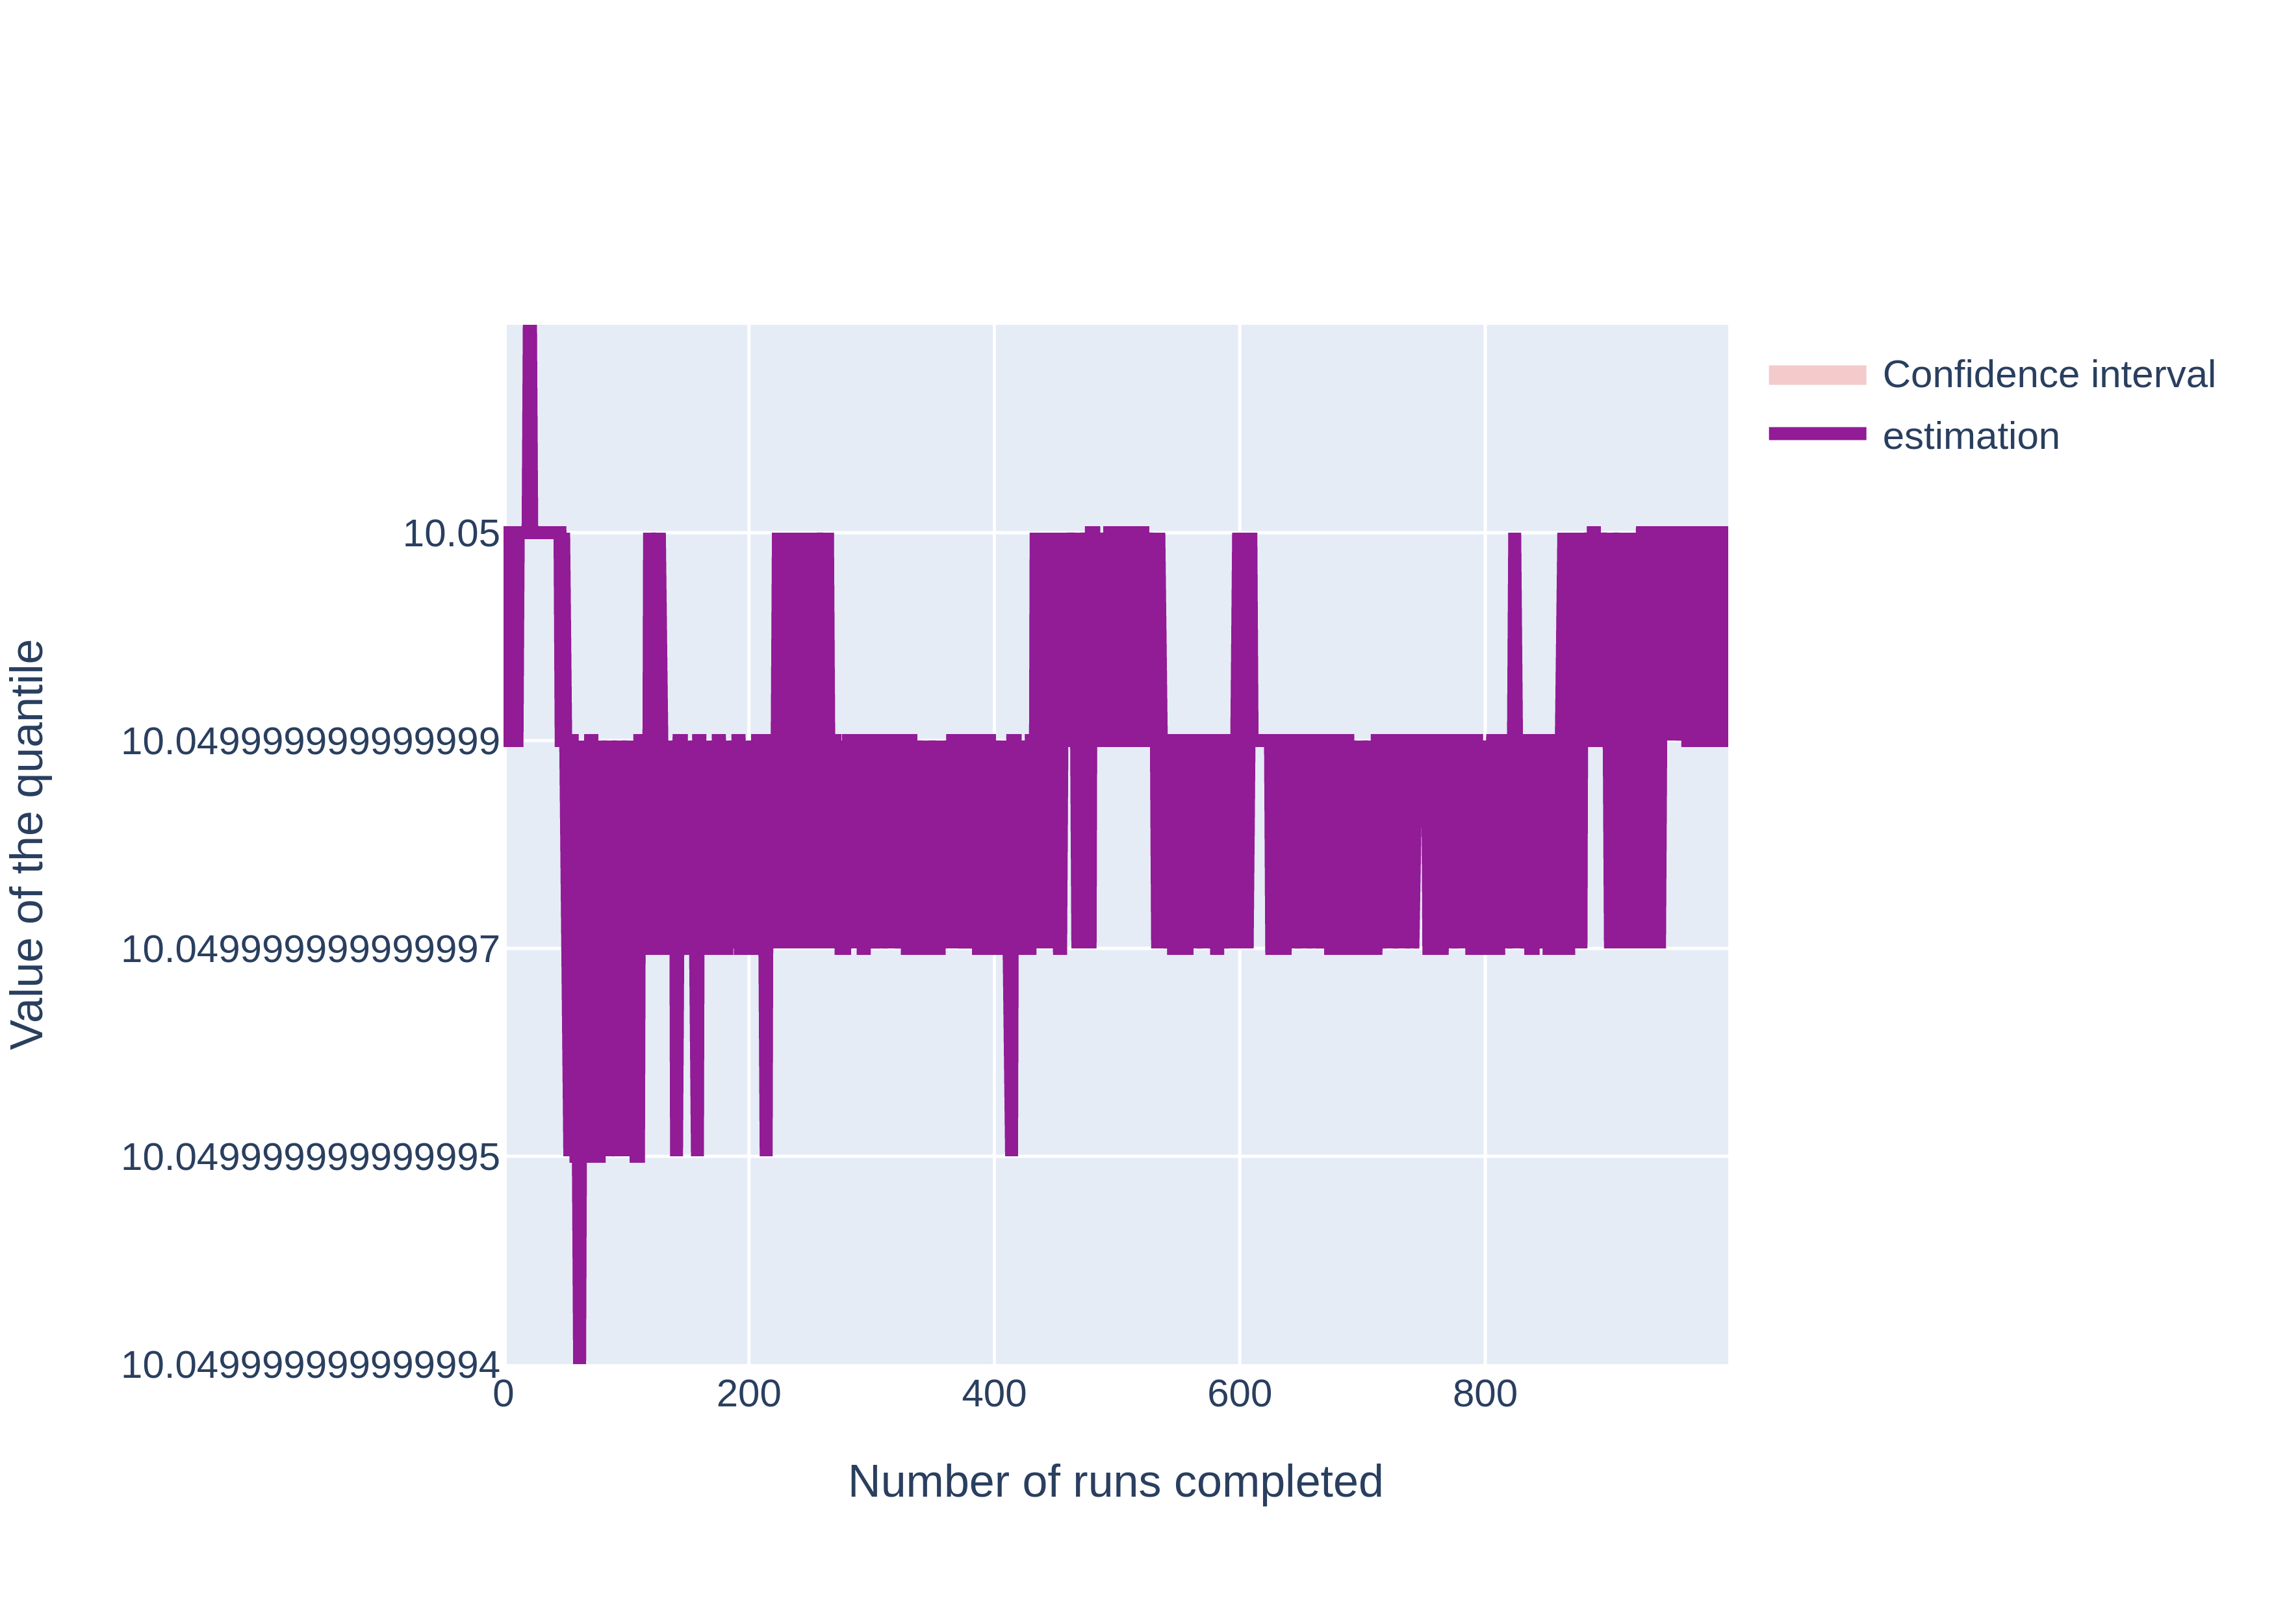
\includegraphics[width=\textwidth]{../fig/quantile4/VD2_4mn.png}
        \caption{Simulation time: 4min}
        \vspace{.5cm}
    \end{subfigure}
    \begin{subfigure}{.495\textwidth}
        \centering
        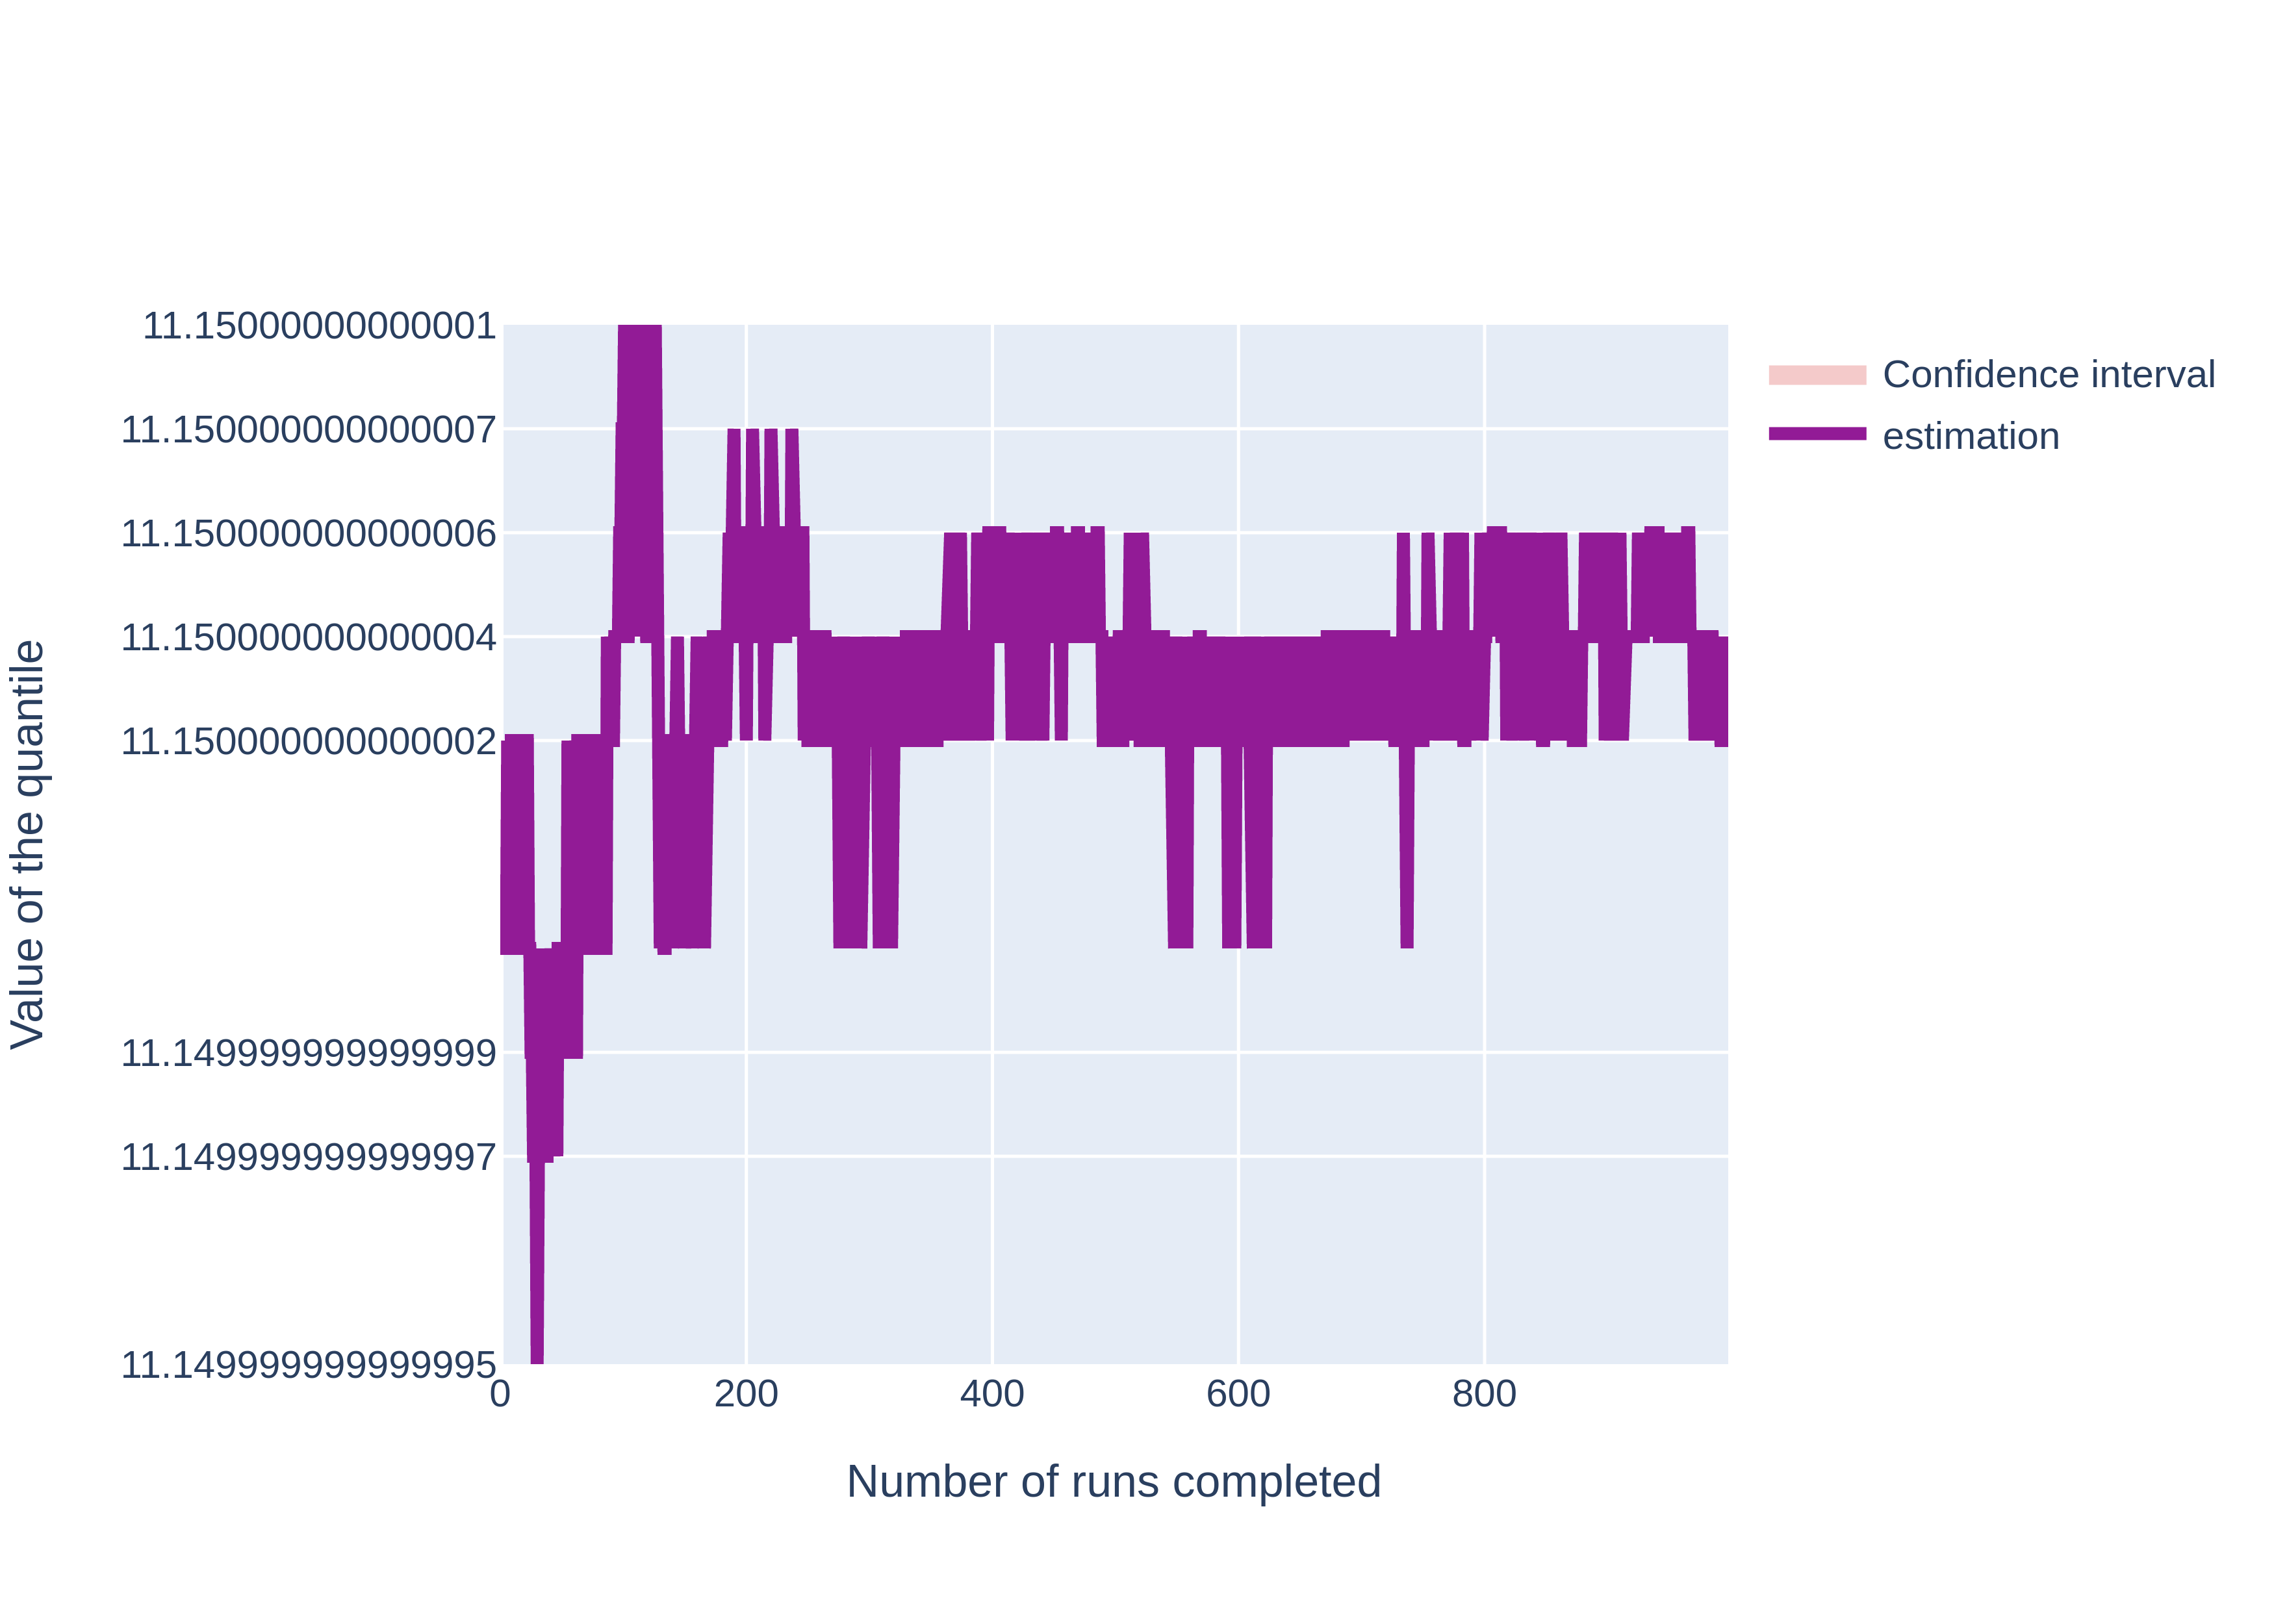
\includegraphics[width=\textwidth]{../fig/quantile4/VD2_40mn.png}
        \caption{Simulation time: 40min}
    \end{subfigure}
    \begin{subfigure}{.495\textwidth}
        \centering
        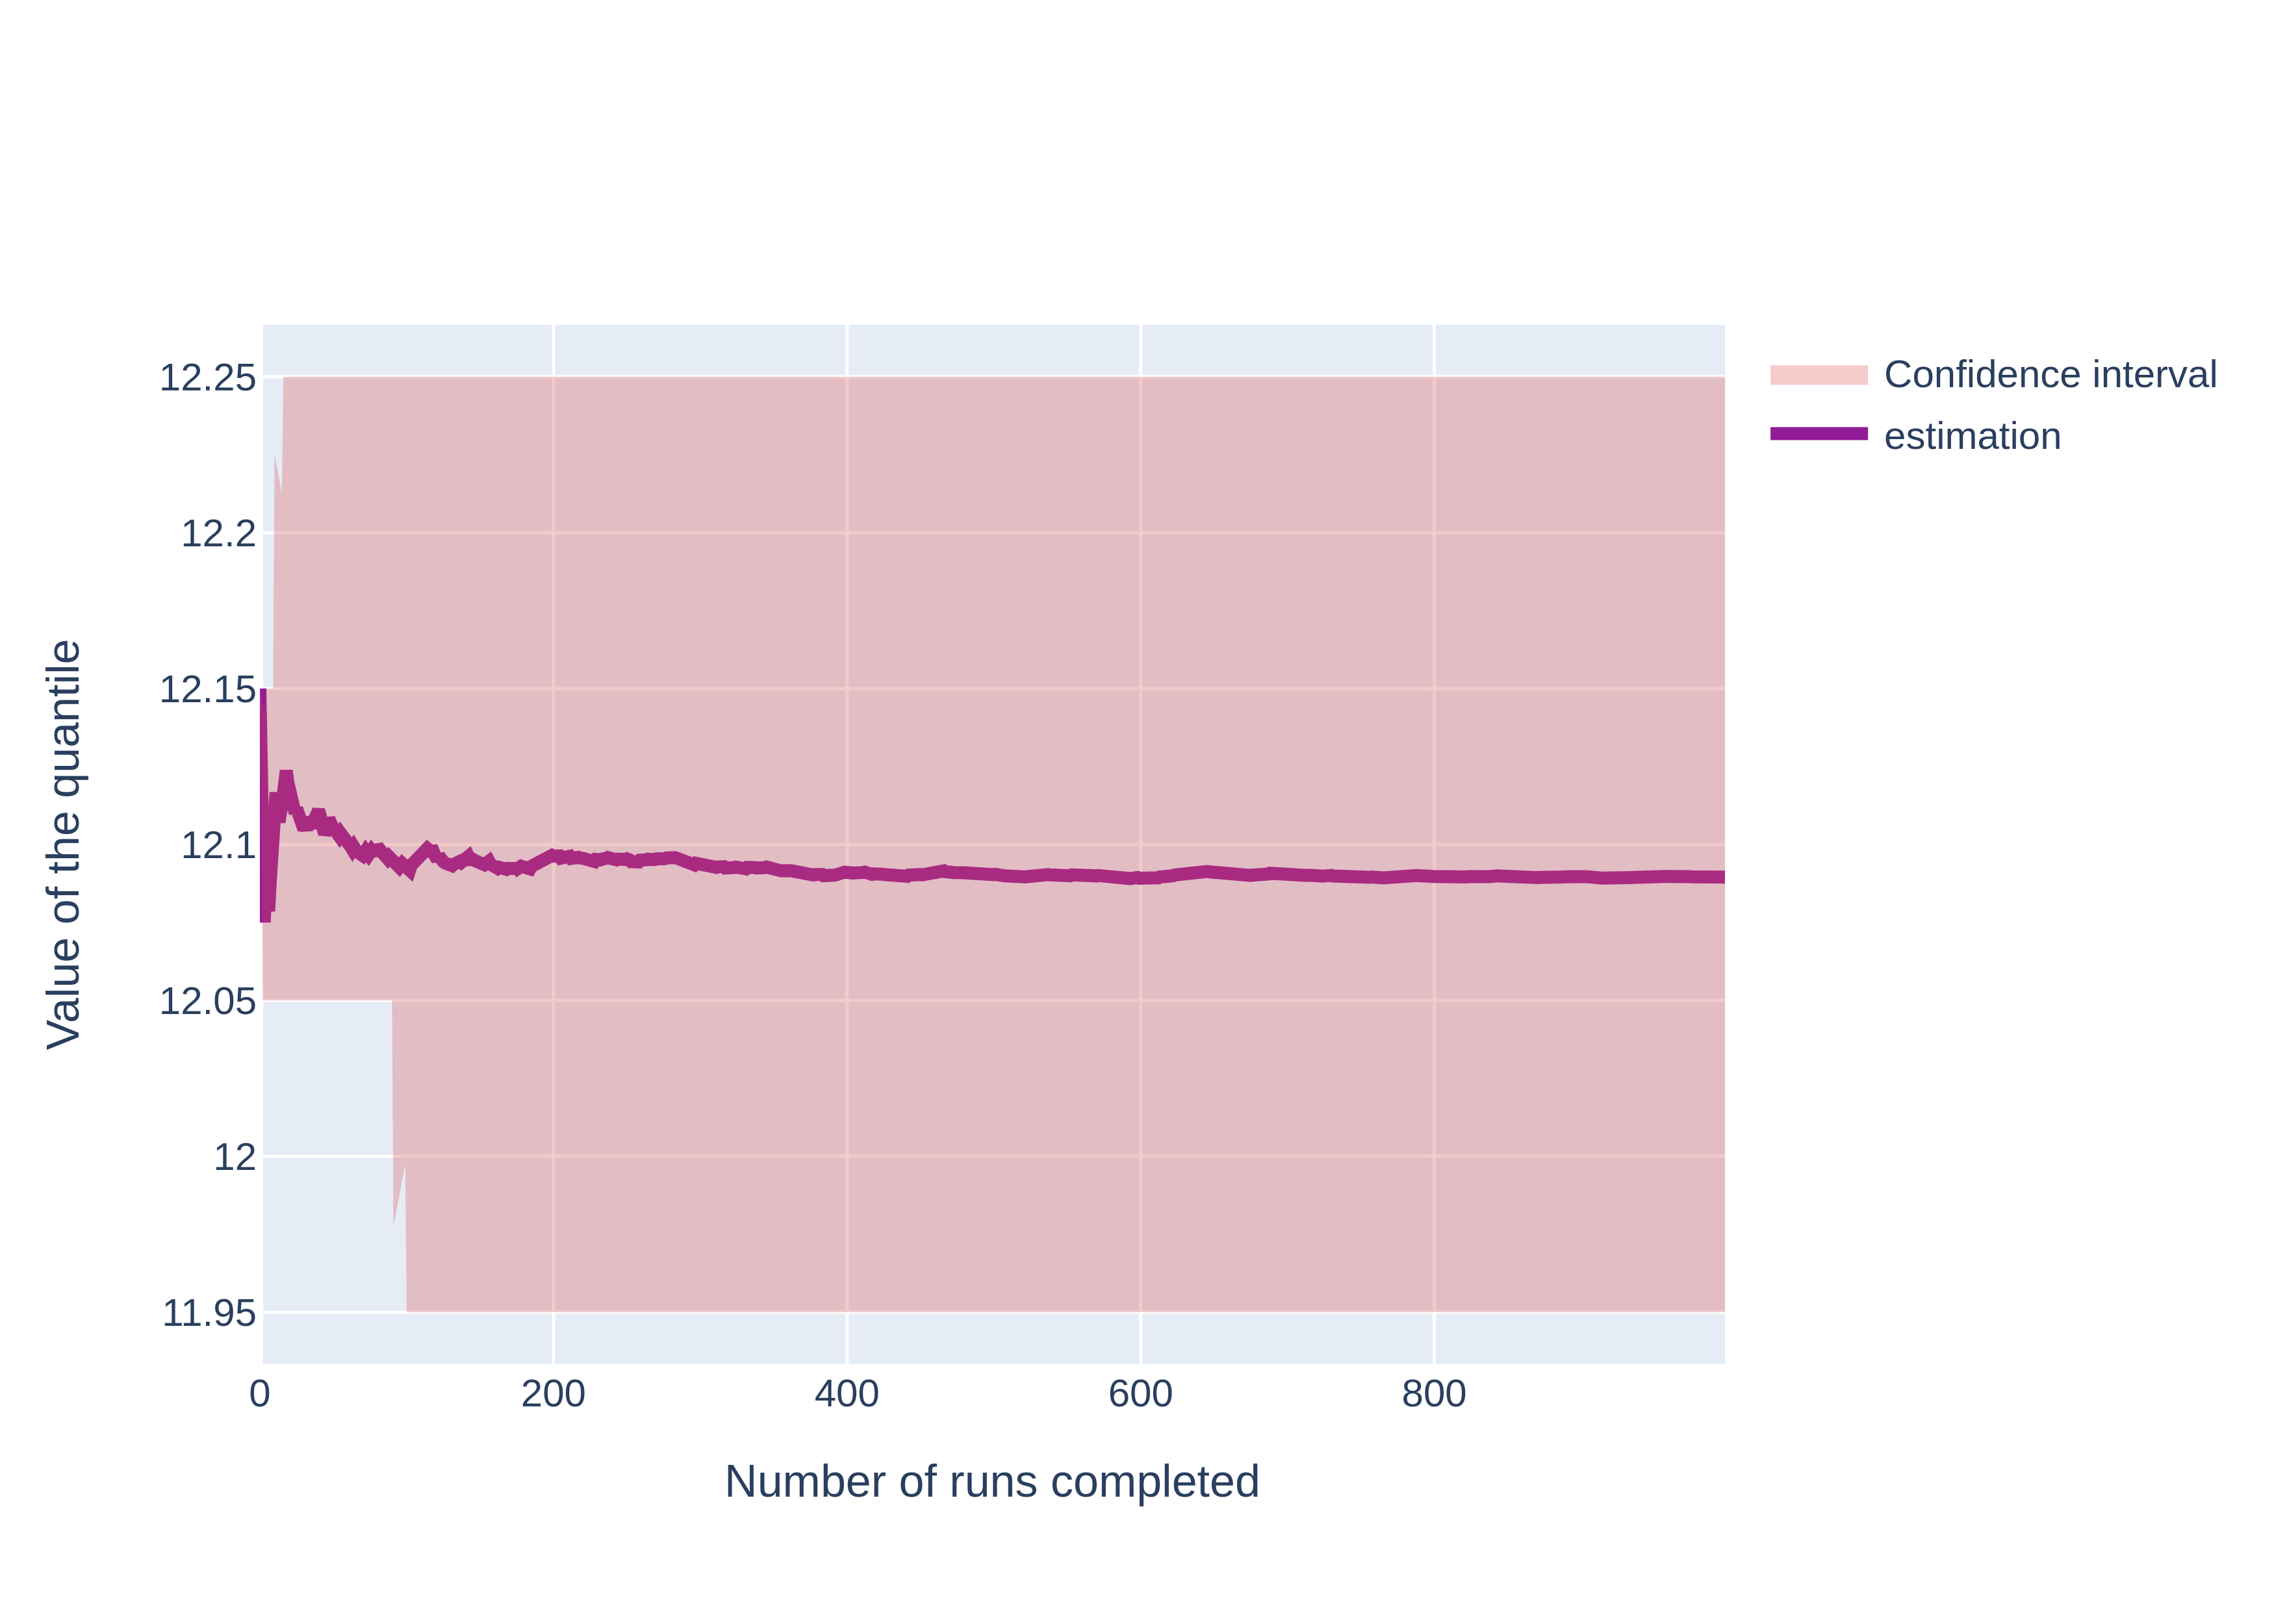
\includegraphics[width=\textwidth]{../fig/quantile4/VD2_400mn.png}
        \caption{Simulation time: 400min}
        \label{fig: VD2 DAT q4 400 min}
    \end{subfigure}
    \caption{VD2 $q_4$ after multiple simulation times}
\end{figure}

\subsubsection{Quantile 5}
\begin{figure}[H]
    \centering
    \begin{subfigure}{.495\textwidth}
        \centering
        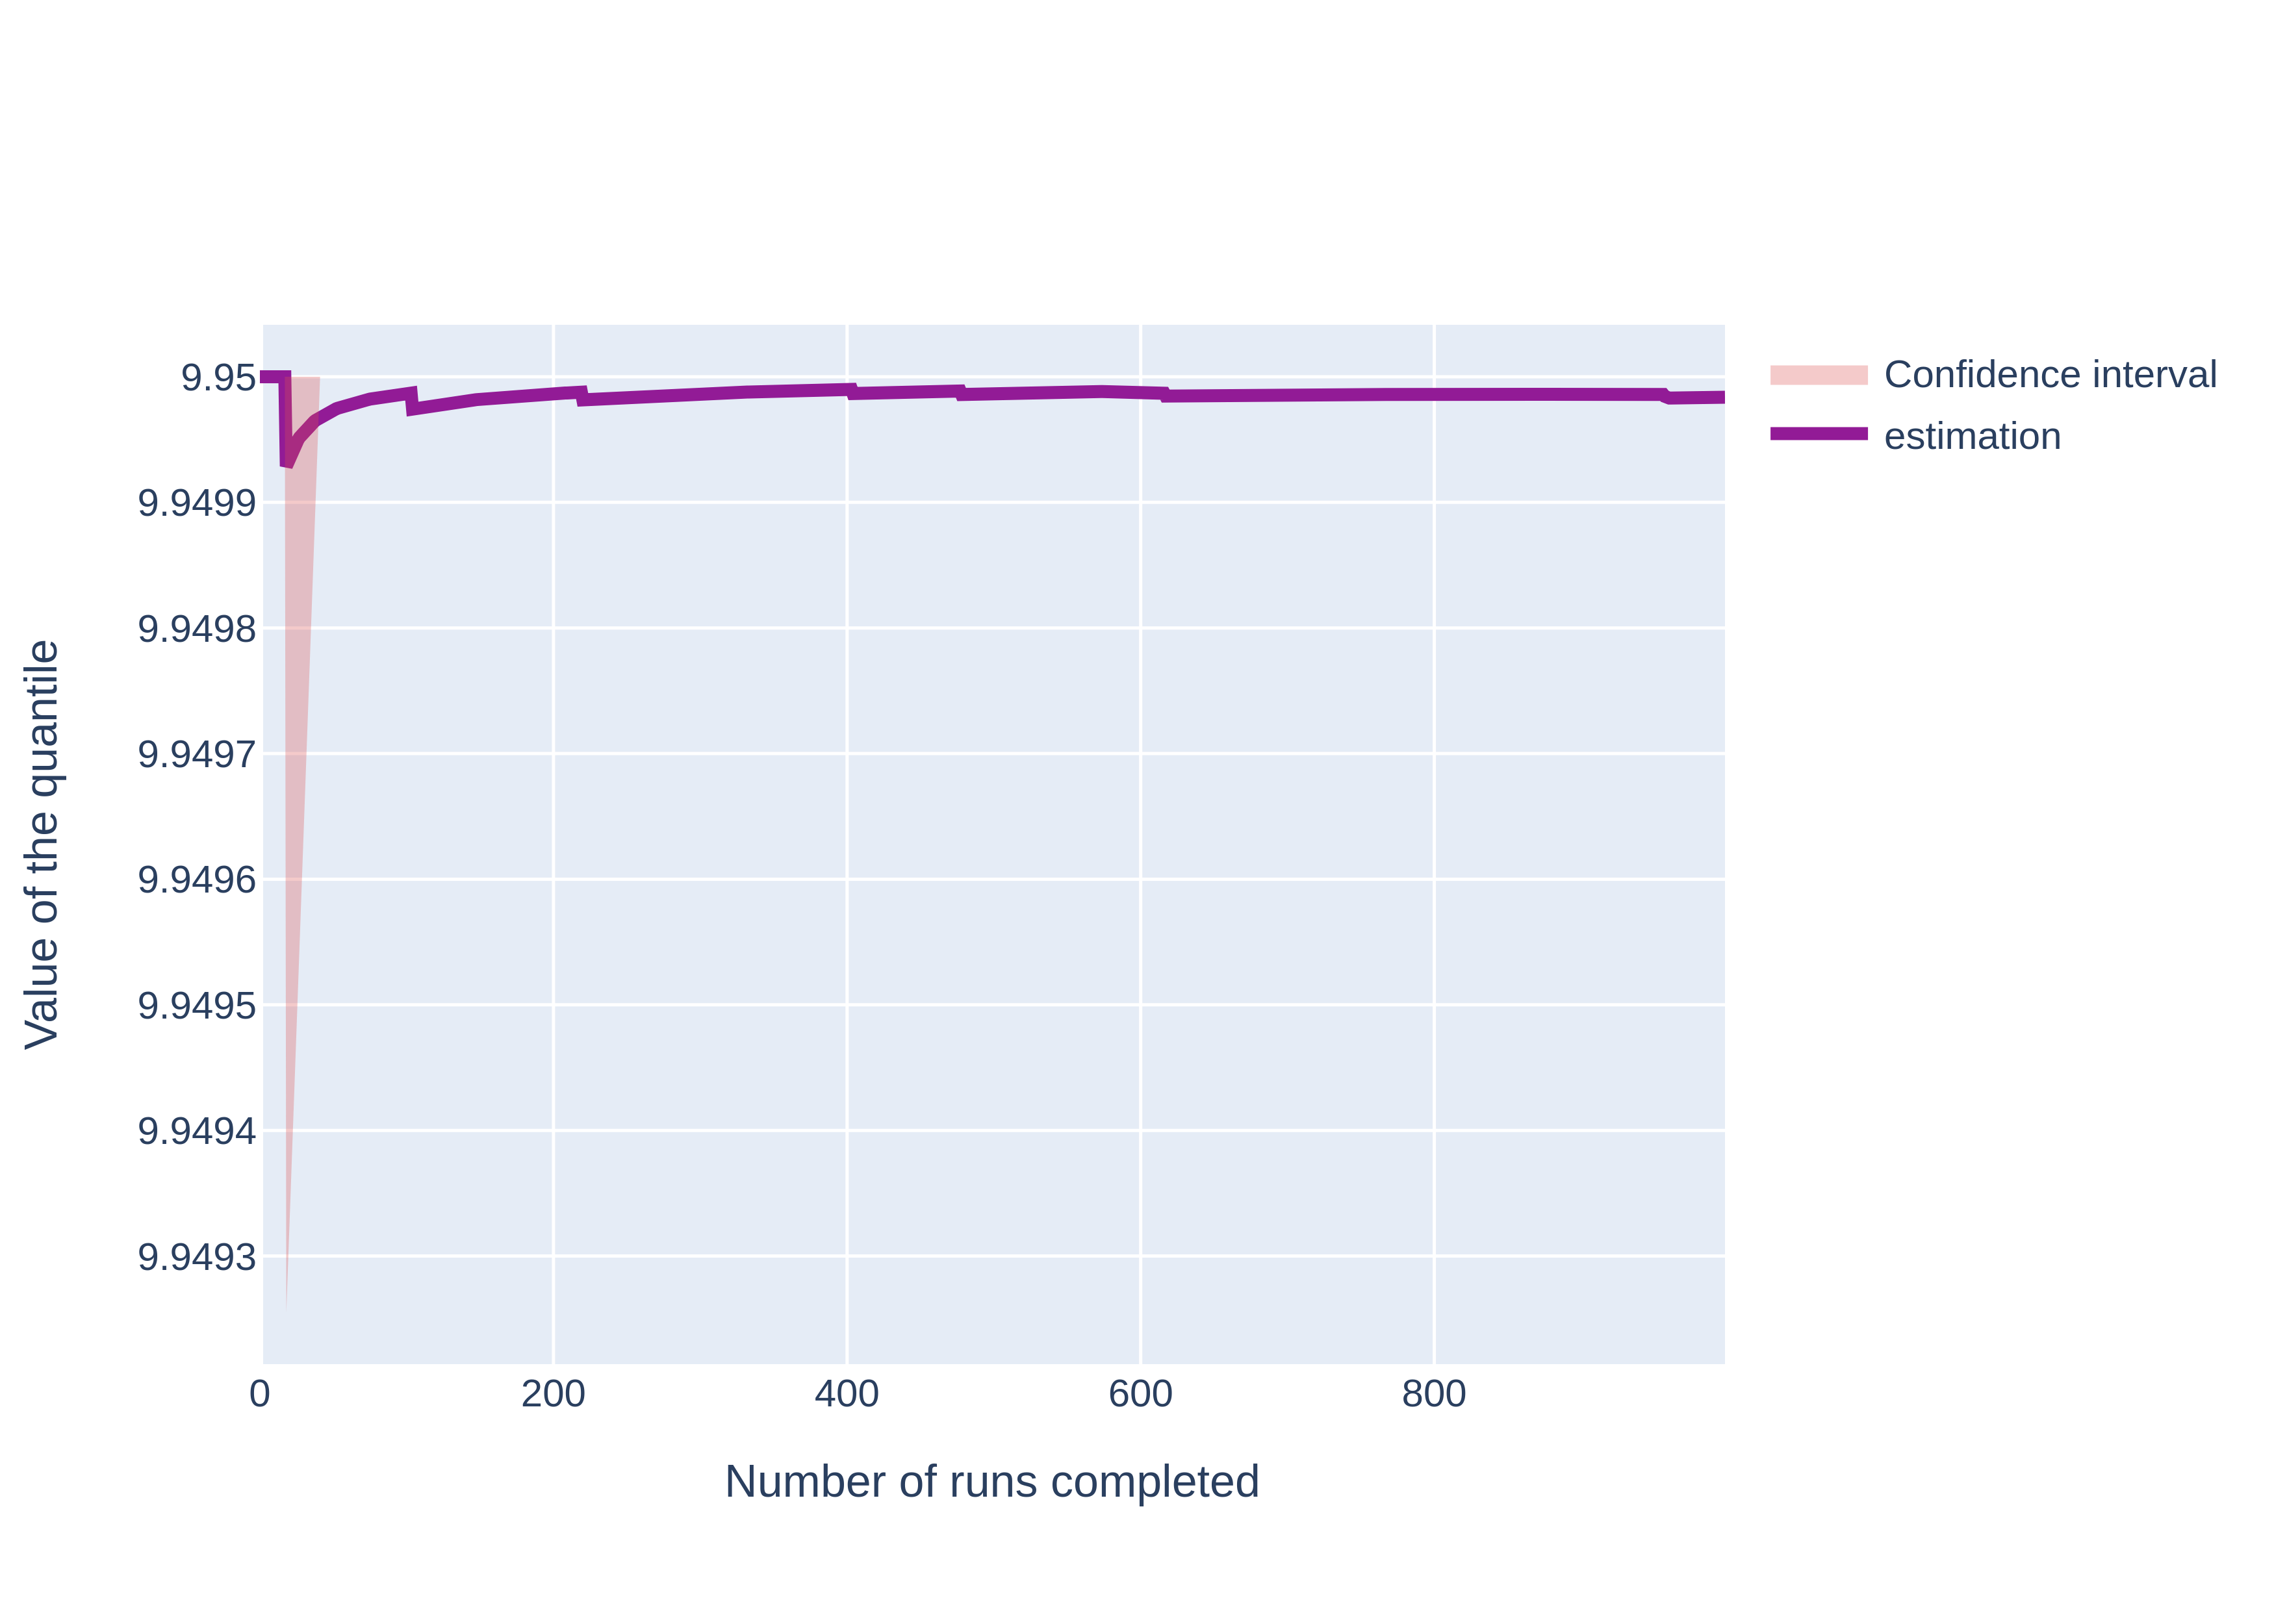
\includegraphics[width=\textwidth]{../fig/quantile5/VD2_24s.png}
        \caption{Simulation time: 24s}
        \vspace{.5cm}
    \end{subfigure}
    \begin{subfigure}{.495\textwidth}
        \centering
        \includegraphics[width=\textwidth]{../fig/quantile5/VD2_4mn.png}
        \caption{Simulation time: 4min}
        \vspace{.5cm}
    \end{subfigure}
    \begin{subfigure}{.495\textwidth}
        \centering
        \includegraphics[width=\textwidth]{../fig/quantile5/VD2_40mn.png}
        \caption{Simulation time: 40min}
    \end{subfigure}
    \begin{subfigure}{.495\textwidth}
        \centering
        \includegraphics[width=\textwidth]{../fig/quantile5/VD2_400mn.png}
        \caption{Simulation time: 400min}
    \end{subfigure}
    \caption{VD2 $q_5$ after multiple simulation times}
\end{figure}




\end{document}